%%%%%%%%%%%%%%%%%%%%%%%%%%%%%%%%%%%%%%%%%%%%%%%%%%%%%%%%%%%%%%%
%% OXFORD THESIS TEMPLATE

% Use this template to produce a standard thesis that meets the Oxford University requirements for DPhil submission
%
% Originally by Keith A. Gillow (gillow@maths.ox.ac.uk), 1997
% Modified by Sam Evans (sam@samuelevansresearch.org), 2007
% Modified by John McManigle (john@oxfordechoes.com), 2015
%
% This version Copyright (c) 2015-2017 John McManigle
%
% Broad permissions are granted to use, modify, and distribute this software
% as specified in the MIT License included in this distribution's LICENSE file.
%

% I've (John) tried to comment this file extensively, so read through it to see how to use the various options.  Remember
% that in LaTeX, any line starting with a % is NOT executed.  Several places below, you have a choice of which line to use
% out of multiple options (eg draft vs final, for PDF vs for binding, etc.)  When you pick one, add a % to the beginning of
% the lines you don't want.


%%%%% CHOOSE PAGE LAYOUT
% The most common choices should be below.  You can also do other things, like replacing "a4paper" with "letterpaper", etc.

% This one will format for two-sided binding (ie left and right pages have mirror margins; blank pages inserted where needed):
% \documentclass[a4paper,twoside]{ociamthesis}
% This one will format for one-sided binding (ie left margin > right margin; no extra blank pages):
% \documentclass[a4paper]{ociamthesis}
% This one will format for PDF output (ie equal margins, no extra blank pages):
\documentclass[a4paper,nobind]{ociamthesis} 



%%%%% SELECT YOUR DRAFT OPTIONS
% Three options going on here; use in any combination.  But remember to turn the first two off before
% generating a PDF to send to the printer!

% This adds a "DRAFT" footer to every normal page.  (The first page of each chapter is not a "normal" page.)
% \fancyfoot[C]{\emph{DRAFT Printed on \today}} 

% This highlights (in blue) corrections marked with (for words) \mccorrect{blah} or (for whole
% paragraphs) \begin{mccorrection} . . . \end{mccorrection}.  This can be useful for sending a PDF of
% your corrected thesis to your examiners for review.  Turn it off, and the blue disappears.
% \correctionstrue


%%%%% BIBLIOGRAPHY SETUP
% Note that your bibliography will require some tweaking depending on your department, preferred format, etc.
% The options included below are just very basic "sciencey" and "humanitiesey" options to get started.
% If you've not used LaTeX before, I recommend reading a little about biblatex/biber and getting started with it.
% If you're already a LaTeX pro and are used to natbib or something, modify as necessary.
% Either way, you'll have to choose and configure an appropriate bibliography format...

% The science-type option: numerical in-text citation with references in order of appearance.
\usepackage[style=numeric-comp, sorting=none, backend=biber, doi=false, isbn=false]{biblatex}
\newcommand*{\bibtitle}{References}
\usepackage{bm}% bold math
\usepackage{mhchem}
% The humanities-type option: author-year in-text citation with an alphabetical works cited.
%\usepackage[style=authoryear, sorting=nyt, backend=biber, maxcitenames=2, useprefix, doi=false, isbn=false]{biblatex}
%\newcommand*{\bibtitle}{Works Cited}

% command to get rid of lines containing URL
% If you want to edit the file in place without creating a temporary file, you can use the sed command:

% bash
% Copy code
% sed -i '/url/d' inputfile.txt
% This command will delete all lines that contain the string 'url' from inputfile.txt without creating a new file. Again, be cautious when using the -i (in-place) option with sed, as it directly modifies the input file.

% This makes the bibliography left-aligned (not 'justified') and slightly smaller font.
\renewcommand*{\bibfont}{\raggedright\small}

% Change this to the name of your .bib file (usually exported from a citation manager like Zotero or EndNote).
% \addbibresource{references_noURL.bib}
\addbibresource{references.bib}

% Uncomment this if you want equation numbers per section (2.3.12), instead of per chapter (2.18):
%\numberwithin{equation}{subsection}

%%%%% THESIS / TITLE PAGE INFORMATION
% Everybody needs to complete the following:
% \title{Patterns and Structures on Biological Membranes}
\title{Models of Protein Organisation}
\author{Matthew W Cotton}
\college{University College}

% Master's candidates who require the alternate title page (with candidate number and word count)
% must also un-comment and complete the following three lines:
%\masterssubmissiontrue
%\candidateno{933516}
%\wordcount{28,815}

% Uncomment the following line if your degree also includes exams (eg most masters):
%\renewcommand{\submittedtext}{Submitted in partial completion of the}
% Your full degree name.  (But remember that DPhils aren't "in" anything.  They're just DPhils.)
\degree{Doctor of Philosophy}
% Term and year of submission, or date if your board requires (eg most masters)
\degreedate{Trinity 2024}


%%%%% YOUR OWN PERSONAL MACROS
% This is a good place to dump your own LaTeX macros as they come up.
\newcommand{\todo}[1]{{\color{red} [#1]}}

% To make text superscripts shortcuts
	\renewcommand{\th}{\textsuperscript{th}} % ex: I won 4\th place
	\newcommand{\nd}{\textsuperscript{nd}}
	\renewcommand{\st}{\textsuperscript{st}}
	\newcommand{\rd}{\textsuperscript{rd}}

%%%%% THE ACTUAL DOCUMENT STARTS HERE
\begin{document}



%%%%% CHOOSE YOUR LINE SPACING HERE
% This is the official option.  Use it for your submission copy and library copy:
% \setlength{\textbaselineskip}{22pt plus2pt}
% This is closer spacing (about 1.5-spaced) that you might prefer for your personal copies:
\setlength{\textbaselineskip}{18pt plus2pt minus1pt}

% You can set the spacing here for the roman-numbered pages (acknowledgements, table of contents, etc.)
\setlength{\frontmatterbaselineskip}{17pt plus1pt minus1pt}

% Leave this line alone; it gets things started for the real document.
\setlength{\baselineskip}{\textbaselineskip}


%%%%% CHOOSE YOUR SECTION NUMBERING DEPTH HERE
% You have two choices.  First, how far down are sections numbered?  (Below that, they're named but
% don't get numbers.)  Second, what level of section appears in the table of contents?  These don't have
% to match: you can have numbered sections that don't show up in the ToC, or unnumbered sections that
% do.  Throughout, 0 = chapter; 1 = section; 2 = subsection; 3 = subsubsection, 4 = paragraph...

% The level that gets a number:
\setcounter{secnumdepth}{2}
% The level that shows up in the ToC:
\setcounter{tocdepth}{2}


%%%%% ABSTRACT SEPARATE
% This is used to create the separate, one-page abstract that you are required to hand into the Exam
% Schools.  You can comment it out to generate a PDF for printing or whatnot.
\begin{abstractseparate}
	Your abstract text goes here.  Check your departmental regulations, but generally this should be less than 300 words.  See the beginning of Chapter~\ref{ch:2-litreview} for more.

Lorem ipsum dolor sit amet, consectetur adipiscing elit. Pellentesque sit amet nibh volutpat, scelerisque nibh a, vehicula neque. Integer placerat nulla massa, et vestibulum velit dignissim id. Ut eget nisi elementum, consectetur nibh in, condimentum velit. Quisque sodales dui ut tempus mattis. Duis malesuada arcu at ligula egestas egestas. Phasellus interdum odio at sapien fringilla scelerisque. Mauris sagittis eleifend sapien, sit amet laoreet felis mollis quis. Pellentesque dui ante, finibus eget blandit sit amet, tincidunt eu neque. Vivamus rutrum dapibus ligula, ut imperdiet lectus tincidunt ac. Pellentesque ac lorem sed diam egestas lobortis.

Proteins are the workhorses of the cell and sub-cellular environments. Recently lots of work has investigated the problem of protein structure, that is, understanding how the sequence of amino acids residues that make up a protein can be mapped to their shape and how this affects function. In this these I look at cooperative effects between proteins. This is a higher level of organisation that occurs due to interactions between proteins giving organisation in space and time and across length scales. I will investigate these processes using mathematical models to understand the key mechanisms that drive the emergent structures we observe. This work is focused on understanding three examples of protein organisation which can then be hijacked for bio-engineering or this understanding can be used to design rational therapeutics for diseases associated with protein organisation. % Create an abstract.tex file in the 'text' folder for your abstract.
\end{abstractseparate}


% JEM: Pages are roman numbered from here, though page numbers are invisible until ToC.  This is in
% keeping with most typesetting conventions.
\begin{romanpages}

% Title page is created here
\maketitle

%%%%% DEDICATION -- If you'd like one, un-comment the following.
%\begin{dedication}
%This thesis is dedicated to\\
%someone\\
%for some special reason\\
%\end{dedication}

%%%%% ACKNOWLEDGEMENTS -- Nothing to do here except comment out if you don't want it.
% \begin{acknowledgements}
%  	\subsection*{Personal}

This is where you thank your advisor, colleagues, and family and friends.

Lorem ipsum dolor sit amet, consectetur adipiscing elit. Vestibulum feugiat et est at accumsan. Praesent sed elit mattis, congue mi sed, porta ipsum. In non ullamcorper lacus. Quisque volutpat tempus ligula ac ultricies. Nam sed erat feugiat, elementum dolor sed, elementum neque. Aliquam eu iaculis est, a sollicitudin augue. Cras id lorem vel purus posuere tempor. Proin tincidunt, sapien non dictum aliquam, ex odio ornare mauris, ultrices viverra nisi magna in lacus. Fusce aliquet molestie massa, ut fringilla purus rutrum consectetur. Nam non nunc tincidunt, rutrum dui sit amet, ornare nunc. Donec cursus tortor vel odio molestie dignissim. Vivamus id mi erat. Duis porttitor diam tempor rutrum porttitor. Lorem ipsum dolor sit amet, consectetur adipiscing elit. Sed condimentum venenatis consectetur. Lorem ipsum dolor sit amet, consectetur adipiscing elit.
% \end{acknowledgements}

%%%%% ABSTRACT -- Nothing to do here except comment out if you don't want it.
% \begin{abstract}
% 	Your abstract text goes here.  Check your departmental regulations, but generally this should be less than 300 words.  See the beginning of Chapter~\ref{ch:2-litreview} for more.

Lorem ipsum dolor sit amet, consectetur adipiscing elit. Pellentesque sit amet nibh volutpat, scelerisque nibh a, vehicula neque. Integer placerat nulla massa, et vestibulum velit dignissim id. Ut eget nisi elementum, consectetur nibh in, condimentum velit. Quisque sodales dui ut tempus mattis. Duis malesuada arcu at ligula egestas egestas. Phasellus interdum odio at sapien fringilla scelerisque. Mauris sagittis eleifend sapien, sit amet laoreet felis mollis quis. Pellentesque dui ante, finibus eget blandit sit amet, tincidunt eu neque. Vivamus rutrum dapibus ligula, ut imperdiet lectus tincidunt ac. Pellentesque ac lorem sed diam egestas lobortis.

Proteins are the workhorses of the cell and sub-cellular environments. Recently lots of work has investigated the problem of protein structure, that is, understanding how the sequence of amino acids residues that make up a protein can be mapped to their shape and how this affects function. In this these I look at cooperative effects between proteins. This is a higher level of organisation that occurs due to interactions between proteins giving organisation in space and time and across length scales. I will investigate these processes using mathematical models to understand the key mechanisms that drive the emergent structures we observe. This work is focused on understanding three examples of protein organisation which can then be hijacked for bio-engineering or this understanding can be used to design rational therapeutics for diseases associated with protein organisation.
% \end{abstract}

%%%%% MINI TABLES
% This lays the groundwork for per-chapter, mini tables of contents.  Comment the following line
% (and remove \minitoc from the chapter files) if you don't want this.  Un-comment either of the
% next two lines if you want a per-chapter list of figures or tables.
\dominitoc % include a mini table of contents
%\dominilof  % include a mini list of figures
%\dominilot  % include a mini list of tables

% This aligns the bottom of the text of each page.  It generally makes things look better.
\flushbottom

% This is where the whole-document ToC appears:
\tableofcontents

% \listoffigures
% 	\mtcaddchapter
% \mtcaddchapter is needed when adding a non-chapter (but chapter-like) entity to avoid confusing minitoc

% Uncomment to generate a list of tables:
%\listoftables
%	\mtcaddchapter

%%%%% LIST OF ABBREVIATIONS
% This example includes a list of abbreviations.  Look at text/abbreviations.tex to see how that file is
% formatted.  The template can handle any kind of list though, so this might be a good place for a
% glossary, etc.
% \include{text/abbreviations}

% The Roman pages, like the Roman Empire, must come to its inevitable close.
\end{romanpages}

%%%%% CHAPTERS
% Add or remove any chapters you'd like here, by file name (excluding '.tex'):
\flushbottom
% \begin{savequote}[8cm]
% \textlatin{Neque porro quisquam est qui dolorem ipsum quia dolor sit amet, consectetur, adipisci velit...}

% There is no one who loves pain itself, who seeks after it and wants to have it, simply because it is pain...
%   \qauthor{--- Cicero's \textit{de Finibus Bonorum et Malorum}}
% \end{savequote}

\chapter{\label{ch:1-intro}Introduction} 

\minitoc
\newpage

Proteins are the molecular building blocks of all living systems. The emergence of life from these fundamental components depends on how proteins are organised in both space and time, and across a magnitude of scales. Understanding the forces governing this organisation not only elucidates how matter comes alive, but knowing how and why these processes go wrong can help us to design effective therapeutics for disease or even hijack and engineer these processes to harness the power of proteins.

In this thesis I explore three different mechanisms for protein organisation. I will develop mathematical models that capture the main features of physical interactions between proteins and study the structure and consequences of these equations, comparing with experimental studies where relevant. Each mechanism has broadly been studied before but I will detail how previous studies have failed to capture key features of the interaction that can lead to a fundamentally different route for protein organisation.

\section{What is a protein}

Proteins are a class of biomolecules that are long unbranched chains of monomer units, called amino acids. \cite{jones2002soft} Each amino acid has the same basic structure that polymerises to form a protein backbone held together by peptide bonds, a type of covalent bond. The distinct amino acids have distinct side chains that are attached to the polymerising unit and it is this side chain that defines the different amino acids. This sequence of amino acids, including their side chains, defines the protein and is referred to as the primary protein structure. An array of non-covalent bonds, such as hydrogen bonds, electrostatic attractions and van der Waals, further define the 3D configuration of the chain in giving the protein a secondary and ternary structure. This ternary structure defines the shape of the protein,  and specifies the location of each atom, although thermal fluctuations induce slight perturbations and prevent proteins from being fixed in this exact configuration. The protein's ternary structure is also crucial in determining the proteins function, for example proteins that catalyse biological reactions, enzymes, do so by binding to a molecule to form a complex. The lock and key model of this binding requires that the enzyme and molecule have exactly complimentary shapes.

these interactions are fundamentally encoded into the DNA o.. information of life

and often the protein's functions specifically depends on this structure which is exactly defined by the genetic information. This is the central dogma of biology: DNA makes RNA, and RNA makes proteins.

The genetic information in an organism's DNA encode for the sequence of amino acids that define the protein. Proteins are manufactured by connected this sequence of amino acids by covalent bonds and this is called the primary protein structure.

Specificity research to try and improve the effect of catalysts to speed up reactions.

Quaternary structure, beyond single proteins we get groups -> can be scaled up to larger enzyme complexes (channelling? perhaps)

Proteins are the work horses of cellular and subcellular machinery. Enzymes are proteins that catalyse reactions, making processes feasible on relevant molecular timescales. Kinesin and other motor proteins drag cargo and provide essential active transport functionality, however proteins such as ion channels can span barriers within the cell and allow passive transport to occur moving. This aresenal of transport processes determines how the distribution of biomolecules is kept from equilibrium, or how efficiently a system can relax to some steady state, helping to control cell signalling and the flow of information. Another function of proteins is as building blocks for subcellular structures such as microtubules or viral capsids \cite{keskin_principles_2008}. If anything happens on the scale of \todo{quantify this scale somehow...} there is normally a protein making to happen.

lots of discussion around sepcificity of enzyme to exact shape of some substrates etc.

phosphorylation of proteins

\begin{figure}
    \centering
    % 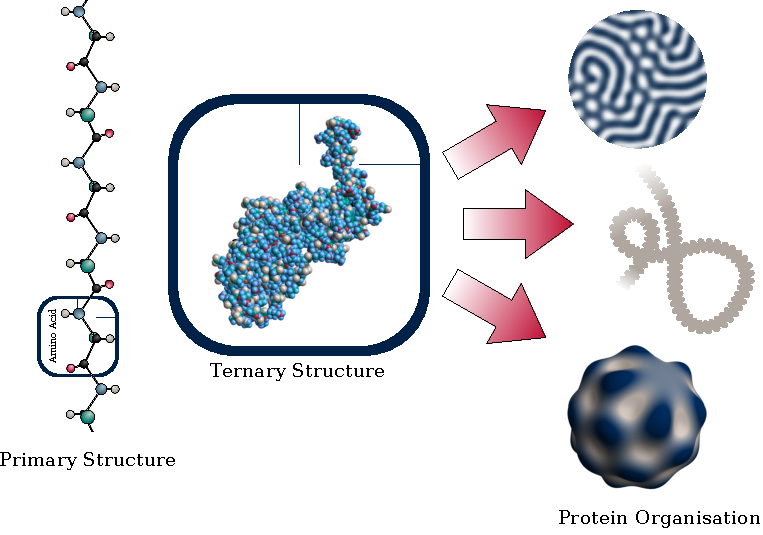
\includegraphics[width=0.8\textwidth]{figures/proteinLevels.pdf}
    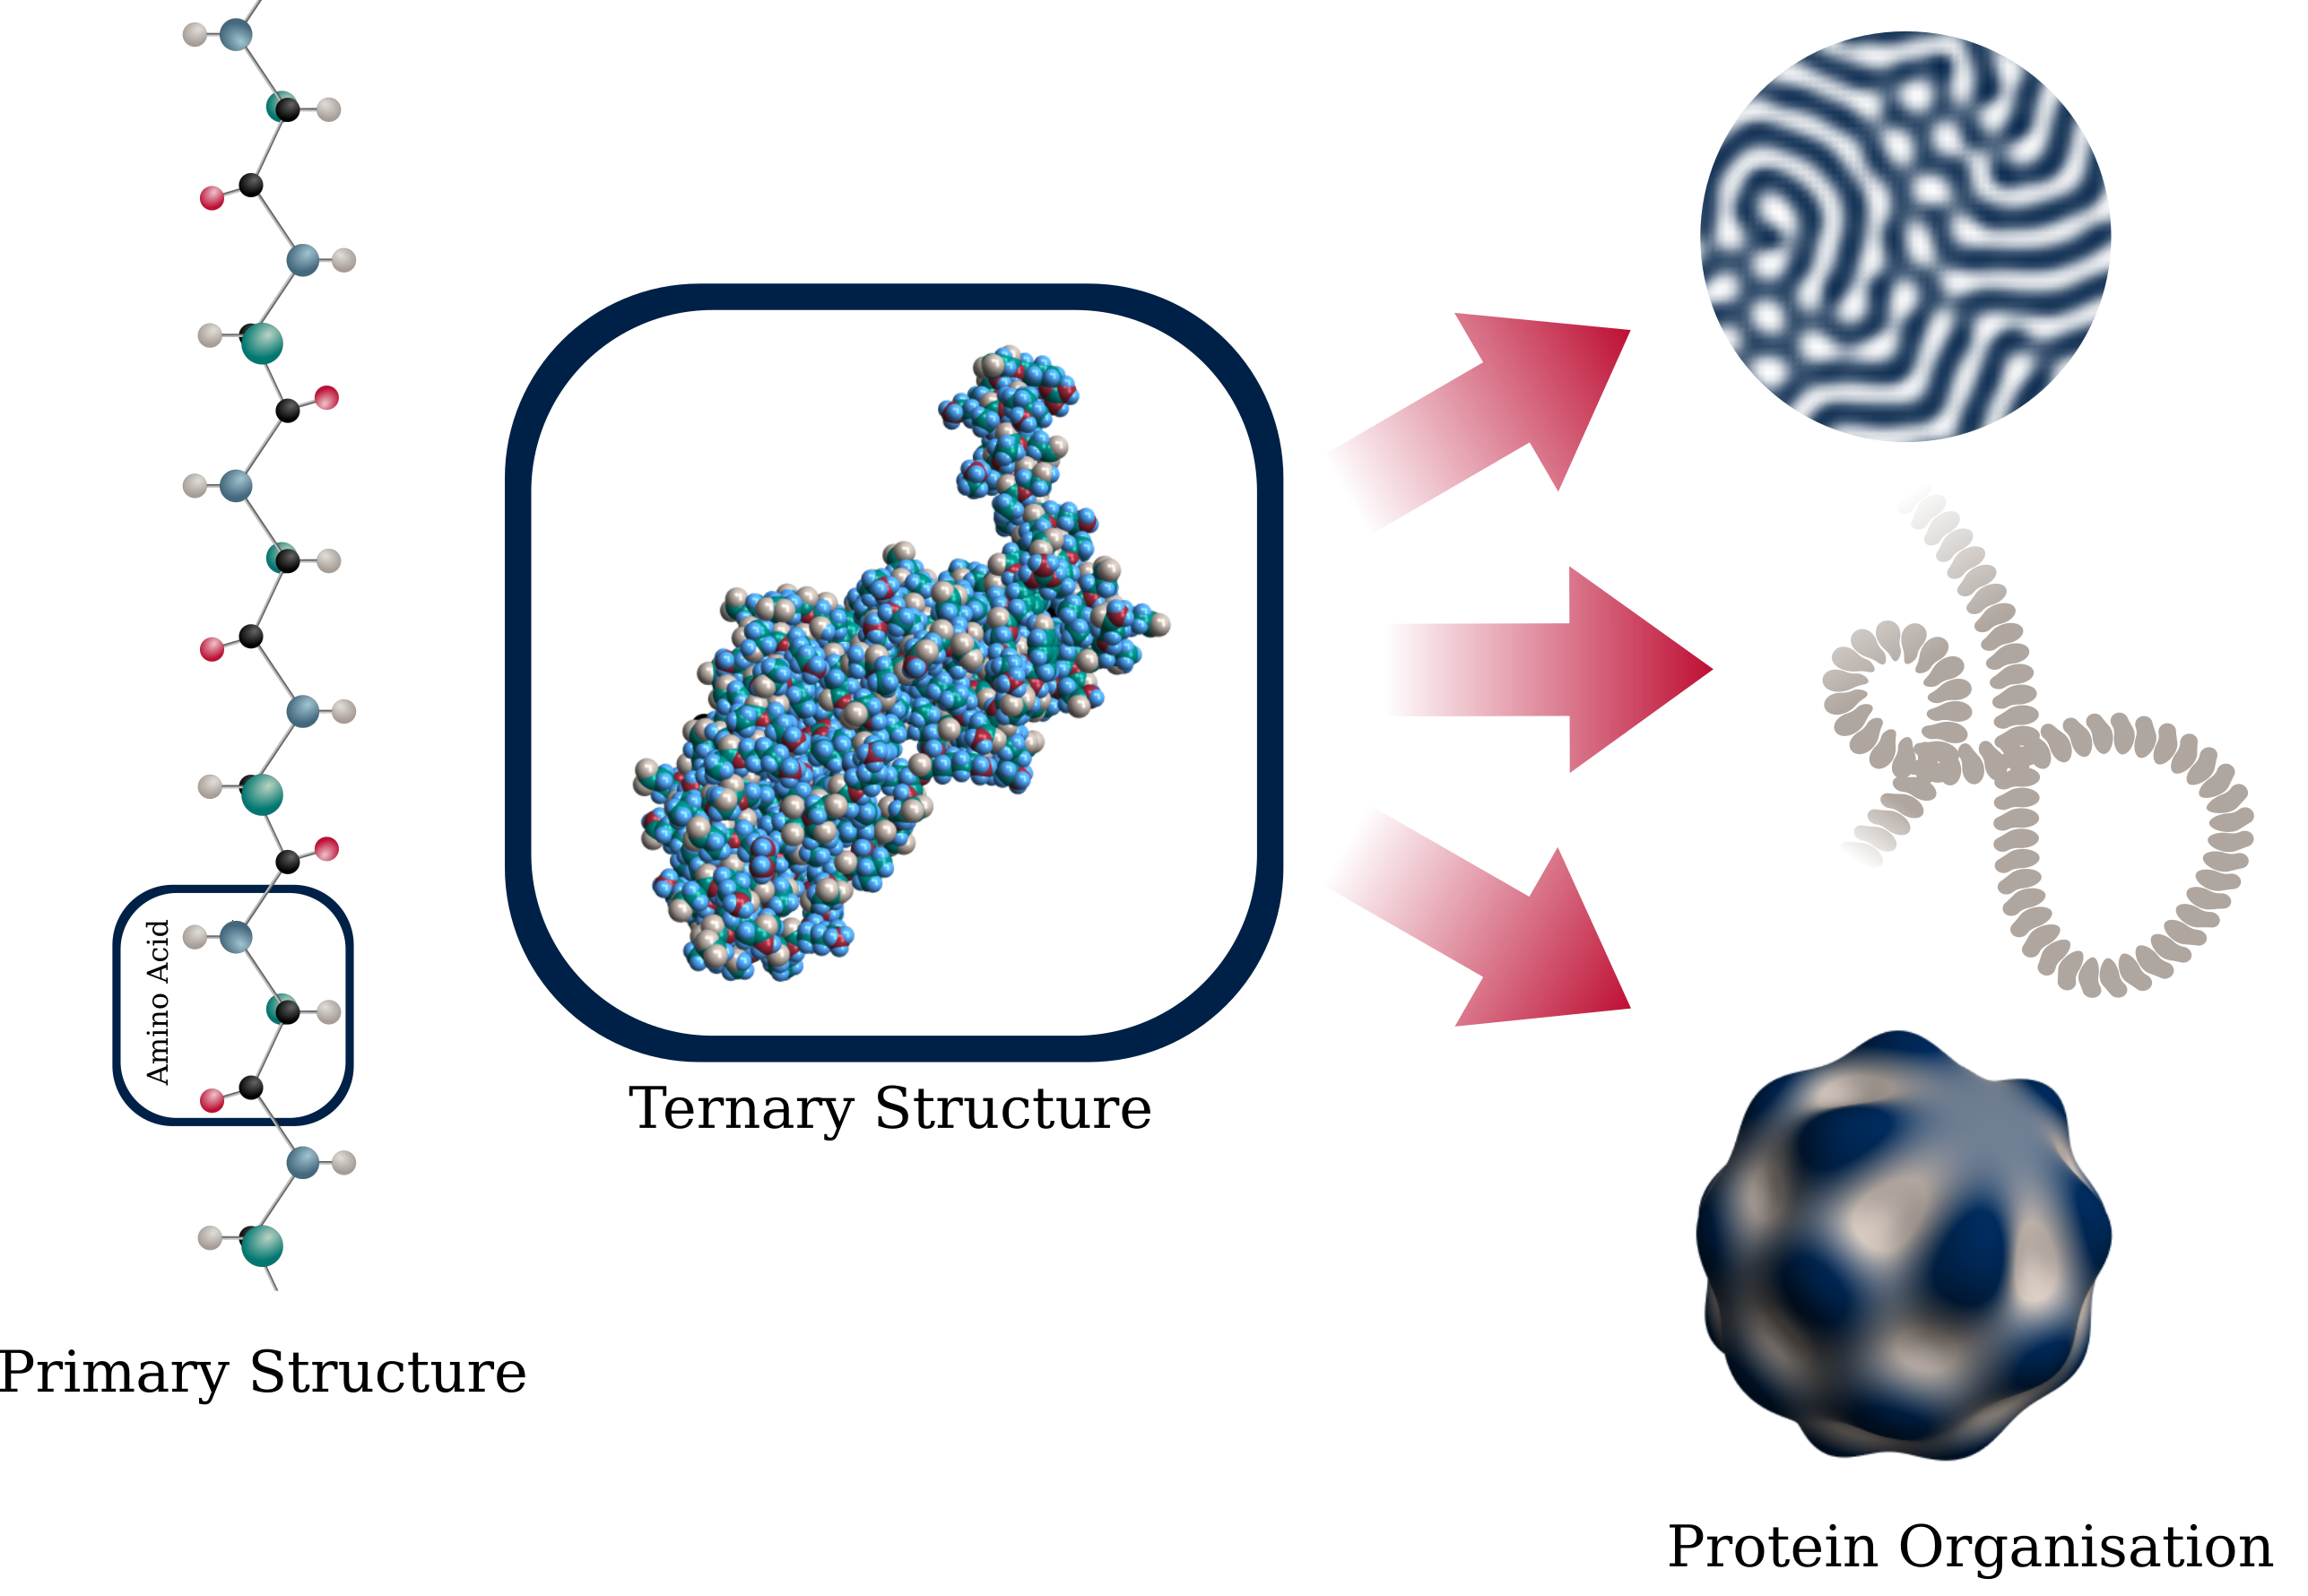
\includegraphics[width=1\textwidth]{figures/proteinLevels.png}
    \caption{The hierarchy of protein structure. Amino acids make proteins that then interact to form structures and patterns. The graphics show examples of protein organisation inspired by (top to bottom) reaction diffusion systems \cite{turing_chemical_1952}, fibrils \todo{ref} and curvature induced membrane patterning \cite{agudo-canalejo_pattern_2017}. The structure of the protein shown is generated from coordinates in the protein database, structure 1EZB, \cite{garrett_solution_1997}}
    \label{fig:1-proteinLevels}
\end{figure}


\section{Proteins in Health and Disease}

\section{Engineering Proteins}

synbio etc.

\section{Protein }
During my DPhil the development and release of AlphaFold changed the conversation around protein structure . AlphaFold is a neural network desigened to solve the problem of protein folding: learning the map from amino acid sequence (primary structure) to an atomistic description of the 3D shape (ternary structure). In 2021, AlphaFold became the first computational method to achieve accuracy on par with experimental structure determination. Since then, it has become an invaluable tool in arsenal of scientists trying to understand a variety of biological processes. Structure prediction can help to understand why a CRISP knockout might stop a molecule binding to a protein, elucidating unknown binding mechanisms, and engineering mutations to enhance binding affinity and catalytic rates. This model also represented a paradigm shift from mechanistic physics informed modelling to solve the folding problem to a deep learning approach. This was possible due to the extensive database of experimentally determined structures in the Protein Data Bank and the abundance of sequencing data from advanced sequencing technologies.

In this thesis, I have explored an alternative approach to protein engineering. Rather than considering changing the individual protein structure, I have explored mechanisms by which proteins can conspire to form structures that affect function. This collective organization often relates to protein structure; for instance, intrinsically disordered domains can drive equilibrium phase separation [and alphafold has helpd i think...]. However, my research demonstrates that the protein environment also plays a crucial role in tuning emergent phenomena. Varying monomer concentration in systems of aggregating proteins, adding solvent to a dense active mixture, or increasing the tension in a membrane filled with proteins are all examples of the rich parameter space that can be engineered when we begin to understand larger scale protein dynamics. 

The physics of these systems and mechanistic modelling remain central to research in this area. Recent studies have used AI etc. to determine the dynamics, but doesnt really give advice about coupleing them, or general downstream effects etc. Also need to determine whats important in each system (tbf AI could probable help with this). However more crucailly, in these cases the question is quite spceific. Here we cant quite do this, the question is less obvious...

What we can do is solve more sepcific question... reaction networks - Vincent + Antonis. But coupling everything together will give the best results...



The current suit of experimental data do not provide sufficient 

The question is less well posed. 

for example disordered regions of protein structure are hard to predict with alphaFold, but are more likely tro 
Intrinsically disordered proteins (pappu reference).
\cite{jumper_highly_2021}
Although not 

Used AI rather than physics based models

an  accuracy that the assessors considered competitive with that of experimental methods

The protein folding problem is now often refereed to as \textit{solved} and the application of \todo{AI} has shifted the focus from physically informed mechanistic models, into

\section{Abstracting and Modelling Proteins}

The space of amino acid chains and therefore of potential proteins is vast. There are \todo{potentially a calculation here?} The massive design space has been exploited by evolution to give a variety of 

Proteins are a fantastic model system for mathematicians and physicists to study. They are small enough to abstract as simple particles, but have sufficient complexity that they can maintain a plethora of reactions as described above. But more recently they can be engineered…

\section{How do proteins interact}

Protein organisation in health and disease

\section{Dump}

Refrerence Jaime’s dimer stuff, I like that PNAS paper

\section{Thesis Scope and Structure}

Each chapter in this thesis explores a different physical mechanism to drive protein organisation. I will introduce the background necessary to understand each mechanism and highlight specific aspects of these protein-protein interactions that have been previously understudied. Using a range of techniques, I will build mathematical models that incorporate this understudied features and study their effects on the resulting protein organisation, and ultimately how this can affect function or pathology. Below I provide a very brief summary of each system studied:
\begin{enumerate}
    \item \textbf{Catalysis Induced Phase Separation} Liquid-liquid phase separation can form droplets in mixtures of proteins and other components. The formation of these regions can be driven by equilibrium interactions between the components, but in this chapter I demonstrate that modelling chemically active components can give rise to fundamentally new phenomena. An enzymatic component can drive liquid-liquid phase separation without the interactions and this can subsequently affect overall reaction rates in the system.
    \item \textbf{Anisotropic Membrane Mediated Interactions} Proteins that bind to and bend biological membranes can generate elastic forces that act on other proteins in the membrane. These forces can generate structures and remodel the membrane. However, many of the proteins that bind in this way break radial symmetry and this changes their interactions, introducing an equilibrium separation and forming lattices of inclusions that can be controlled via the protein curvature or membrane tension.
    \item \textbf{Bounded clearance in Neurodegenerative Disease}\todo{could use actual chapter titles and enumerate with chapter numbers perhaps?} A plethora of neurodegenrative diseases are associated with aggregated proteins that are produced and removed in the brain. However, existing models ignore physical constraints that limits and bounds the rates at which these aggregated proteins can be removed. Including this key limit when modelling the aggregation kinetics can present a fundamentally new mechanism for the onset of disease which is consistent with recent experiments and can help design rational therapeutics.
\end{enumerate}
% \begin{savequote}[8cm]
% Alles Gescheite ist schon gedacht worden.\\
% Man muss nur versuchen, es noch einmal zu denken.

% All intelligent thoughts have already been thought;\\
% what is necessary is only to try to think them again.
%   \qauthor{--- Johann Wolfgang von Goethe \cite{von_goethe_wilhelm_1829}}
% \end{savequote}

% From the CIPS paper

\newcommand{\kcat}[0]{k_{\mathrm{cat}}}
\newcommand{\kspo}[0]{k_{\mathrm{spo}}}
\newcommand{\rcat}[0]{r_{\mathrm{cat}}}
\newcommand{\rspo}[0]{r_{\mathrm{spo}}}

\newcommand{\Rs}[0]{R_\mathrm{s}}
\newcommand{\Rp}[0]{R_\mathrm{p}}
\newcommand{\Ree}[0]{R_\mathrm{e}}

\newcommand{\phie}[0]{\phi_{\mathrm{e}}}
\newcommand{\phis}[0]{\phi_{\mathrm{s}}}
\newcommand{\phip}[0]{\phi_{\mathrm{p}}}
\newcommand{\phisp}[0]{\phi_{\mathrm{s+p}}}
\newcommand{\phiw}[0]{\phi_{\mathrm{w}}}

\newcommand{\mue}[0]{\mu_{\mathrm{e}}}
\newcommand{\muf}[0]{\mu_{\mathrm{f}}}
\newcommand{\mus}[0]{\mu_{\mathrm{s}}}
\newcommand{\mup}[0]{\mu_{\mathrm{p}}}
\newcommand{\muw}[0]{\mu_{\mathrm{w}}}

\newcommand{\Des}[0]{D_{\mathrm{es}}}
\newcommand{\Dse}[0]{D_{\mathrm{se}}}
\newcommand{\Dep}[0]{D_{\mathrm{ep}}}
\newcommand{\Dpe}[0]{D_{\mathrm{pe}}}
\newcommand{\Dsp}[0]{D_{\mathrm{sp}}}
\newcommand{\Dps}[0]{D_{\mathrm{ps}}}
\newcommand{\Dew}[0]{D_{\mathrm{ew}}}
\newcommand{\Dsw}[0]{D_{\mathrm{sw}}}
\newcommand{\Dpw}[0]{D_{\mathrm{pw}}}

\newcommand{\Mee}[0]{M_{\mathrm{ee}}}
\newcommand{\Mes}[0]{M_{\mathrm{es}}}
\newcommand{\Mep}[0]{M_{\mathrm{ep}}}
\newcommand{\Mse}[0]{M_{\mathrm{se}}}
\newcommand{\Mss}[0]{M_{\mathrm{ss}}}
\newcommand{\Msp}[0]{M_{\mathrm{sp}}}
\newcommand{\Mpe}[0]{M_{\mathrm{pe}}}
\newcommand{\Mps}[0]{M_{\mathrm{ps}}}
\newcommand{\Mpp}[0]{M_{\mathrm{pp}}}
\newcommand{\Mwp}[0]{M_{\mathrm{wp}}}
\newcommand{\Mws}[0]{M_{\mathrm{ws}}}
\newcommand{\Mwe}[0]{M_{\mathrm{we}}}


\newcommand{\vp}[0]{v_{\mathrm{p}}}
\newcommand{\vs}[0]{v_{\mathrm{s}}}
\newcommand{\ve}[0]{v_{\mathrm{e}}}
\newcommand{\vw}[0]{v_{\mathrm{w}}}

\newcommand{\ex}[1]{\mathrm{e}^{#1}}
\newcommand{\kb}[0]{k_{\rm B}}

\chapter{\label{ch:2-draft}Active Phase Separation of Dense Mixtures}

\minitoc
\newpage

\section{Introduction}

A lipid bilayer model with only one lipid component can undergo a melting transition, yet a lipid mixture can show phase coexistence, even with as little as two phospholipids and a cholesterol component \cite{elson_phase_2010}. Model cell membranes, made of these mixtures, result in regions of a liquid ordered and liquid disordered phase, and depending on the lipid composition, additional gel phases can also appear \cite{sych_how_2021, aufderhorst-roberts_three-phase_2017}. Lipid-lipid and lipid-cholesterol interactions can drive the well mixed system to form these separate domains, where the proportion of saturated and unsaturated lipids differ in each domain and the size of the domains can be either macroscopic or nanoscopic depending on composition \cite{feigenson_phase_2009}. Temperature dependent interactions built on equilibrium models of phase separating systems can predict the phase behaviour \cite{wolff_thermodynamic_2011}, however in these model systems the amount of lipid is conserved. In vivo, local lipid composition actually changes due to membrane recycling and as a result of the activity of enzymes which catalyse lipid synthesis and breakdown \cite{feigenson_phase_2009}. These features are not incorporated into existing theory, but could give rise to additional spatial organisation in living membranes.

Theoretical models describing the physics of of liquid-liquid phase separation have developed significantly in recent years, partly driven by the observation of membraneless organelles in vivo \cite{shin_liquid_2017}. A key development in the field has been to add non-equilibrium effects into descriptions of phase transitions including, actively propelled particles \cite{cates_motility-induced_2015}, phoretic transport effects \cite{agudo-canalejo_active_2019} and changes in chemical composition \cite{weber_drops_2021, li_non-equilibrium_2020}. The role of membranes and their interplay with phase separated droplets has also been an exciting area of research, through wetting and remodelling of vesicle membranes by liquid droplets \cite{mangiarotti_wetting_2023}. However this chapter focuses on the organisation of lipids in the plane of a membrane rather than coupling membrane effects to external droplets. In order to capture the effects of changes in composition, this chapter explores ideas from non-equilibrium phase transitions and develops a minimal model to describe an active mixture containing an enzyme component such as might be found from enzymes embedded in phospholipid bilayers \cite{alberts_molecular_2008}.

\section{Equilibrium Phase Separation}

\subsection{Thermodynamics of Fluid Mixtures}

A good example to explore the theory of phase separating mixtures is to study a fluid made up of two components, say, component $A$ and component $B$. To make this mixture, we mix $N_A$ molecules of component $A$ and $N_B$ molecules of component $B$ to give a mixture of total volume $V = v_A N_A + v_B N_B$, where $v_i$ is the specific volume of the component, the \textit{size} of each molecule. The volume fraction of a component, $\phi_i$, in some region of volume, $v$, is defined to be $\phi_i = v_i N_i/v$ and for the two component mixture with constant volume everywhere $\phi_A+\phi_B = 1$. To simplify the notation, let $\phi_A=\phi$ and $\phi_B=1-\phi$, and the volume fraction $\phi$ now describes the proportion of the fluid volume that is component $A$. For an incompressible fluid, the total volume is constant and the relevant free energy is the Helmholtz free energy, $F(N_A, N_B, T)$ where $T$ is the temperature of the fluid. The Helmholtz Free energy is an extensive quantity and so for a homogeneous mixture $F(N_A, N_B, T) = V f(\phi, T)$ where $f(\phi, T)$ is the free energy density and this free energy density determines the phase behaviour of the mixture. If a system phase separates into two coexisting phases, then the free energy of two phase system is $V_{\mathrm{I}} f(\phi_{\mathrm{I}}, T)+ V_{\mathrm{II}} f(\phi_{\mathrm{II}}, T)$ where the two phases are labelled $\mathrm{I}$ and $\mathrm{II}$ and the total volume of the system is conserved $V = V_{\mathrm{I}}+V_{\mathrm{II}}$. It is necessary for the two phase free energy to be lower than the free energy of an equivalent homogeneous system in order for the system to phase separate \cite{jones2002soft}.

In addition to lowering the free energy of the system, any phase separating regions of a mixture must also be in mechanical and chemical equilibrium, otherwise they would exchange components or volume to reach two equilibrated phases. Chemical equilibrium is achieved when the chemical potential, $\mu$ of each component in each phase is constant and so moving a particle across the phase boundary will not change the free energy, $\mu_i^{\mathrm{I}}=\mu_i^{\mathrm{II}}$. The chemical potential for component $i$ is given by
\begin{equation}
    \mu_i = \left(\frac{\partial F}{\partial N_i}\right)_{V, T} = v_i \left(\frac{\partial f}{\partial \phi_i}\right)_{T}.
    \label{eq:2-mu_def}
\end{equation}
The mechanical equilibrium is achieved when the osmotic pressure, $\Pi$ between the two phases is equal, $\Pi^{\mathrm{I}}=\Pi^{\mathrm{II}}$, where the osmotic pressure is given by
\begin{equation}
    \Pi(\phi) = -\left(\frac{\partial F}{\partial V}\right)_{T, N_A} = -f + \phi \left(\frac{\partial f}{\partial \phi}\right)_{T}.
    \label{eq:2-Pi_def}
\end{equation}
since $\phi = N_A v_a/V$ and so $\frac{\partial \phi}{\partial V} = -\phi/V$ \cite{doi_soft_2013}. These conditions have a convenient graphical interpretation. The equation for a tangent to the curve $f(\phi)$ at $\phi=\Tilde{\phi}$ can be written as $y=mx+c$. Equations (\ref{eq:2-mu_def}) and (\ref{eq:2-Pi_def}) give $y=\mu_A(\Tilde{\phi})\phi - \Pi(\Tilde{\phi})$ and as these thermodynamic quantities must be the same for two coexisting phases, we find that two phases can only coexist if they have a \textit{common tangent}! Figure \ref{fig:phase_sep_scheme} highlights the graphical interpretation of these conditions, where plotting $f(\phi)$ can illuminate the phase behaviour of a mixture. A well mixed homogeneous system prepared with volume fraction $\phi^*$, will therefore be stable as two phase separated with regions volume fraction $\phi_{\mathrm{I}}$ and $\phi_{\mathrm{II}}$ ($\phi_{\mathrm{I}} < \phi_{\mathrm{II}}$) given that $\phi_{\mathrm{I}} < \phi^* < \phi_{\mathrm{II}}$ \cite{weber2019physics}. The conservation of $N_A$ requires $V\phi^* = V_{\mathrm{I}}\phi_{\mathrm{I}} +V_{\mathrm{II}}\phi_{\mathrm{II}}$ and volume conservation gives $V = V_{\mathrm{I}}+V_{\mathrm{II}}$ which determines the volumes of each phase

\begin{equation}
    V_{\mathrm{I}} = \frac{\phi_{\mathrm{II}}-\phi^*}{\phi_{\mathrm{II}}-\phi_{\mathrm{I}}}V
    \quad
    \textrm{and}
    \quad
    V_{\mathrm{II}} = \frac{\phi^*-\phi_{\mathrm{I}}}{\phi_{\mathrm{II}}-\phi_{\mathrm{I}}}V.
\end{equation}

\begin{figure}
    \centering
    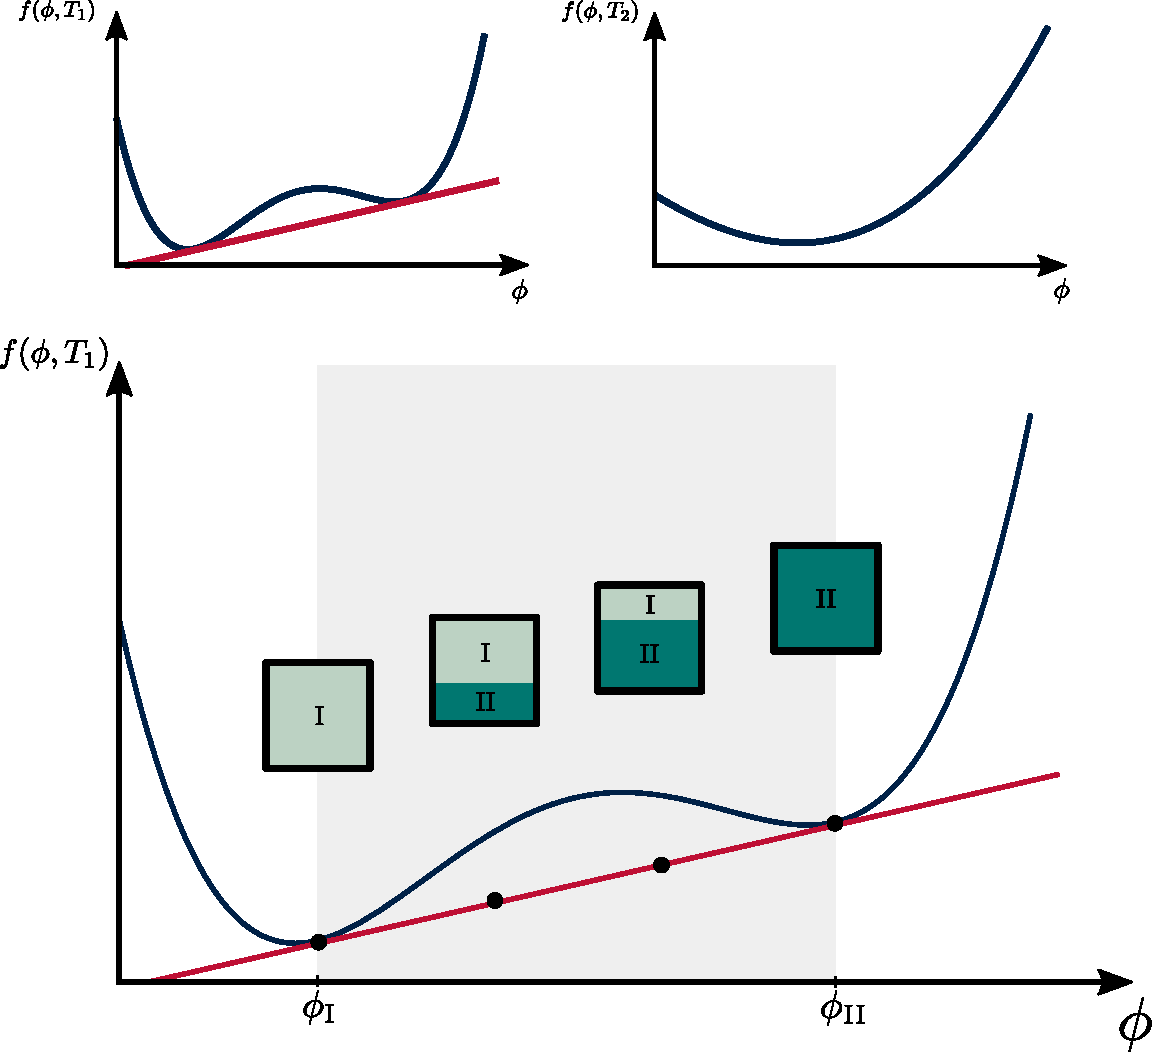
\includegraphics[width=\textwidth]{figures/thermo_solutions.pdf}
    \caption{Schematic of equilibrium phase separation, showing a system that exhibits coexisting phases at some temperature $T_{A}$, but not at another temperature $T_{B}$ which has a convex free energy. In the lower plot examples of the distribution of the two phases in a system are shown with two examples of a phase separated system.}
    \label{fig:phase_sep_scheme}
\end{figure}

Often, the shape of the free energy density can be controlled by some external parameter, such as temperature. When the temperature and consequently the free energy is changed, the two volumes fraction of the coexisting phases also changes. Calculating the the two phases ($\phi_{\mathrm{I}}$ and $\phi_{\mathrm{II}}$) as the temperature changes sweeps out a loci of points called the binondal curve. This is shown graphically in figure \ref{fig:bino_spino_scheme}.

Another important feature of a free energy landscape is the spinodal curve. This curve defines the region where the free energy is unstable, $\frac{\partial^2 f}{\partial \phi^2} > 0$. As such, a mixture in the spinodal region is unstable to small perturbations and will decay into the phase separated state spontaneously. There also exists a region in between the spinodal and binodal curves that is metastable: the free energy would be lower in a phase separated system, but there is an energy barrier preventing the system from transitioning to this state. A large enough pertubation, for example from temperature fluctuations could overcome this nucleation barrier, but often in real systems imperfections, or external structures, can act as nucleation sites and cause the transition. This region is also shown in figures \ref{fig:phase_sep_scheme} and \ref{fig:bino_spino_scheme}, where the shaded region is the unstable spinodal region and the boundary defines the spinodal curve \cite{jones2002soft}.

\begin{figure}
    \centering
    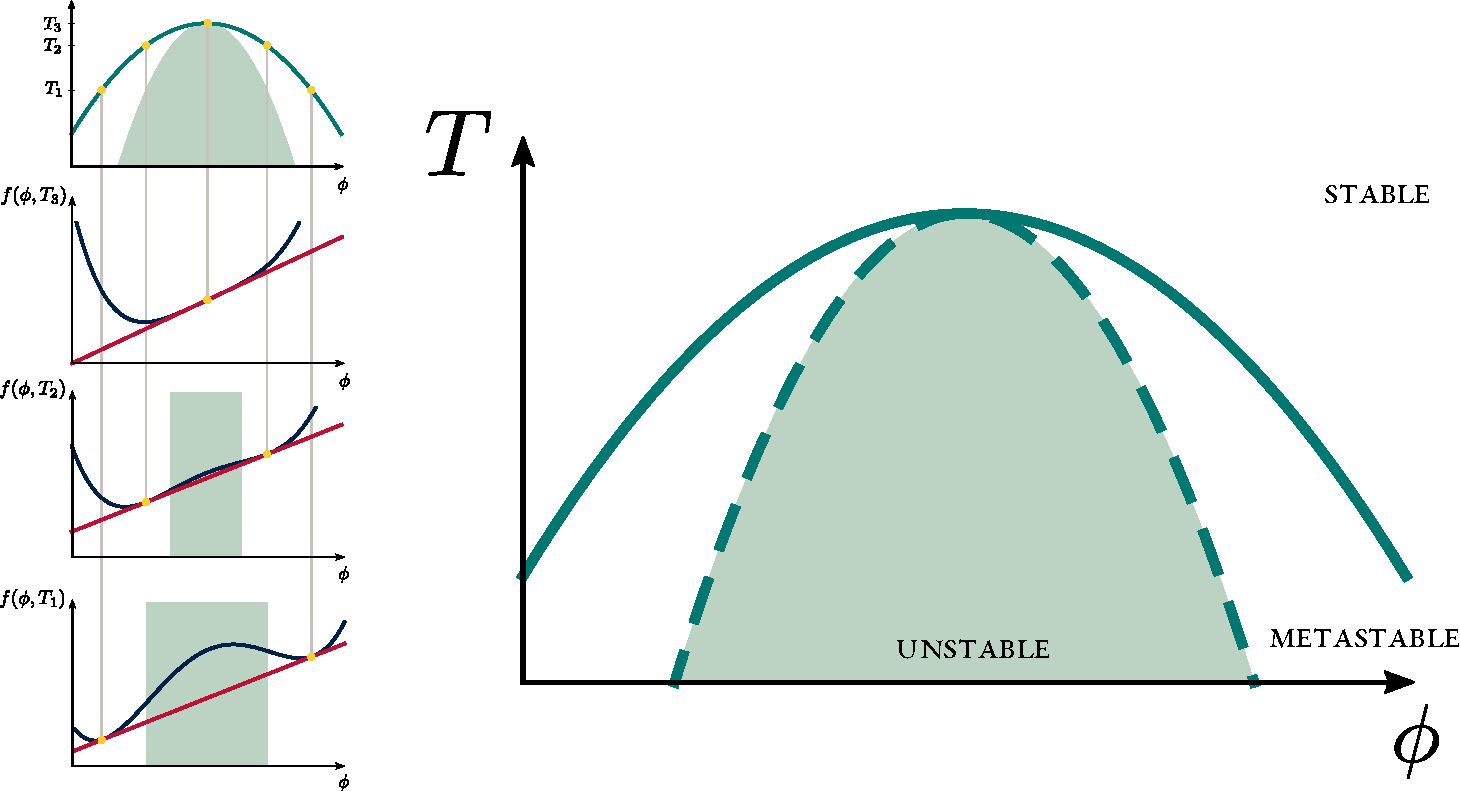
\includegraphics[width=0.9\textwidth]{figures/bino_spino_scheme.pdf}
    \caption{Graphical explanation of how the phase diagram for an equilibrium system is calculated. The solid, binodal line is the boundary between the stable and metastable state and the dashed spinodal line is the boundary between the unstable and metastable states. The two lines meet at the critical point.}
    \label{fig:bino_spino_scheme}
\end{figure}


\subsection{Regular Solution Model}
Mean field models of mixtures can describe the free energy density and predict features of the phase behaviour. Coarse grained order parameters, such as volume fractions provide a useful description of the system, where the volume fraction describes the local  composition, but may not be homogeneous in the system. These order parameters describe the dynamics of an intermediate scale, much larger than the individual lattice sites and much smaller than the overall system size.
The free energy density can be calculated from the Hamiltonian of a system and, again, the $A-B$ binary mixture is a useful place to start. Consider a lattice where each lattice site is occupied by either a molecule of $A$ or a molecule of $B$ where $v_A$ and $v_B$ (the size of each molecule) is the same and is equal to one lattice site. The total number of sites in the lattice  is $N_{lat} = N_A + N_B$. The different molecules can be configured in many different ways on the lattice however the different configurations will have different energies due to interactions between the molecules. The lattice model can include these interactions by having different contributions to the energy for different pairs of molecules on neighbouring lattice sites. For example, two molecules of $A$ on neighbouring sites will contribute $\epsilon_{AA}$ to the energy of a configuration, two molecules of $B$ contribute $\epsilon_{BB}$ and a molecule of $A$ on a neighbouring lattice site to a molecule of $B$ will contribute $\epsilon_{AB}$. The total energy of a configuration $c$ is then the sum of the interaction energy contribution over all neighbouring lattice sites
\begin{equation}
    E_{c} = N_c^{AA}\epsilon_{AA} + N_c^{AB}\epsilon_{AB} + N_c^{BB}\epsilon_{BB}
\end{equation}
where $N_c^{ij}$ is the number of neighbouring lattice site pairs, occupied by a molecule of $i$ and molecule of $j$ in the configuration. The free energy desnity can be calculated from the partition function, $Z$, as
\begin{equation}
    f(\phi, T) = -\frac{\kb T}{V}\ln Z
    \label{eq:2-f_ln}
\end{equation}
where $\kb$ is the Boltzmann constant \cite{kardar2007statistical}. The partition function is directly calculated for a canonical ensemble via
\begin{equation}
    Z = \sum_c \exp{(-\beta E_c)}.
\end{equation}
where $\beta = 1/\kb T$ and the sum is over all configurations. In the thermodynamic limit of large $N_{lat}$ the sum can be well approximated by a mean field approximation. The sum is approximated by replacing the energy of each configuration with the average energy, $\bar{E}$, so the sum now becomes
\begin{equation}
    Z \approx \sum_c \exp(-\beta \bar{E}) = \Omega \exp(-\beta \bar{E})
\end{equation}
where $\Omega$ is the number of unique configurations of molecules on the lattice and is given by
\begin{equation}
    \Omega = \frac{N_{lat}!}{N_A! N_B!}.
\end{equation}

The free energy density in the mean field model is now, with equation (\ref{eq:2-f_ln}), $f = -\frac{K_B T}{V} (\ln \Omega + \bar{E})$.

The mean energy $\bar{E}$ can be calculated in the mean field model. The coordination number, $z$, describes the number of nearest neighbours of each lattice site, for example $z=4$ in a square lattice. On average $z\phi_i$ of the neighbouring lattice sites will be occupied by a molecule of $i$. For $i \neq j$ the average number of $ij$ neighbour pairs, $\bar{N}^{ij}$, is the number of sites occupied by a molecule of $i$ multiplied by the average the number of neighbouring lattice sites occupied by a molecule of $j$: $\bar{N}^{ij} = N_{lat}\phi_i \times z\phi_j$. When $i=j$ each pair will be double counted (each lattice site occupied by a molecule of $i$ will be considered as both the `main' and `neighbour' site) and so there is an additional factor of 1/2 to prevent double counting \cite{doi_soft_2013}. The average energy is therefore
\begin{equation}
\begin{split}
    \bar{E} &= \bar{N}^{AA}\epsilon_{AA} + \bar{N}^{AB}\epsilon_{AB} + \bar{N}^{BB}\epsilon_{BB}\\
    &= \frac{1}{2}z N_{lat} \phi^2\epsilon_{AA} + z N_{lat} (1-\phi)\phi\epsilon_{AB} + \frac{1}{2}z N_{lat} (1-\phi)^2 \epsilon_{BB}.
\end{split}
\end{equation}
Using equation (\ref{eq:2-f_ln}) the free energy density is
\begin{equation}
    f(\phi, T) = -\frac{\kb T}{V}\left(\ln \left(\frac{N_{lat}!}{N_A! N_B!} \right) - \frac{z N_{lat}}{2} \left(\phi^2\epsilon_{AA} + 2(1-\phi)\phi\epsilon_{AB} + (1-\phi)^2 \epsilon_{BB}\right)\right).
\end{equation}
The first term is simplified using Stirling's formula, $\ln N! = N \ln N - N$ for large $N$ to give $\ln\Omega=-N_{lat}(\phi\ln(\phi)+(1-\phi)\ln(1-\phi))$. The average energy term can be simplified as the phase behaviour is independent of the exact value of $f$, or $\partial f/\partial \phi$ and so the physics of the system is symmetric under a transform $f \rightarrow f + k_1 + k_2\phi$. Specifically, choosing $k_1 = z\epsilon_{BB}/2$ and $k_2 = z(\epsilon_{BB} - \epsilon_{AA})/2$ the free energy now becomes
\begin{equation}
    \frac{f(\phi, T)}{\kb T} = \phi\ln(\phi)+(1-\phi)\ln(1-\phi) + \chi(1-\phi)\phi
    \label{eq:2-fh_free}
\end{equation}
since $V = N_{lat}$ and define the Flory-Huggins interaction parameter $\chi = -\frac{z}{2 k_B T} (\epsilon_{AA} + \epsilon_{BB} - 2\epsilon_{AB})$, which is the energy change when a molecule of A is taken from an environment of pure A and put into an evnironment of pure B --- for $\chi<0$ it is energetically favourable for the components to mix and for $\chi>0$ it is favourable for the components to remain separate. The spinodal region can be found by directly calculating the $\frac{\partial^2f}{\partial\phi^2}$ and this shows the existence of a critical point at $\phi_\text{crit}=0.5$ and $\chi_\text{crit}=2$ and so for $\chi<2$ the system cannot phase separate. The critical point must occur $\phi_\text{crit}=0.5$ as the system is symmetric under exchange of $A, B \rightarrow B, A$, however the homogeneous system can be stable for all $\phi$ even when mixed interactions are unfavourable $\chi>0$. This is because when $0<\chi<2$, the entropic terms in the free energy contribute more than the cost of the interactions and so the system remains stable. In equilibrium theories of phase separation it is the interactions that drive the phase behaviour.

\subsubsection{Generalisations of the Regular Solution Free Energy}

The Flory-Huggins theory gives the free energy of a binary mixture in equation (\ref{eq:2-fh_free}), however a similar form of the free energy can be extended to describe a broader class of mixtures. Consider a system of $N$ components, where the mixture is made up of volume fraction $\phi_i$ of component $i$ and $i$ runs from $1$ to $N$. In a system with non-conserved particle number (such as an active system discussed later) the free energy will have additional enthalpic terms. This is intrinsic energy from chemical bonds in a molecule of each species and this contributes linearly in volume fraction to the free energy to give
\begin{equation}
    f_\text{enth} = \sum_{i}\varepsilon_i \frac{\phi_i}{v_i}
\end{equation}
where $\varepsilon_i$ is the enthalpy per molecule of component $i$. If different components in the system have molecules that occupy more than one lattice site, then the previous calculation of $\Omega$, the number of microstates, is overestimated, as nearby sites will necessarily be occupied by the same molecule. This modifies the entropic contribution to the free energy and the Flory-Huggins theory gives the entropic contribution as
\begin{equation}
    f_\text{entr} = \sum_{i}\kb T \frac{\phi_i}{v_i}\ln\phi_i
\end{equation}
as if a molecule is larger, then there are fewer molecules per volume and therefore fewer microstates. Volume effects will also appear in the calculation of the chemical potential, due to the conversion between volume fraction and the number of molecules
\begin{equation}
    \mu_i = \frac{\partial F}{\partial N_i} = v_i\frac{\partial F}{\partial \phi_i}.
\end{equation}
For a mixture of $N$ components the full theory will describe interactions between all components so that the contribution to the free energy from interactions becomes
\begin{equation}
    f_\text{int} = \sum_{i, j}\frac{\chi_{ij}}{2}\phi_i\phi_j.
\end{equation}
where the sum denotes the double sum running from $0$ to $N$ for both indices, the factor of $1/2$ means each interaction is only counted once and the scalar interaction parameter, $\chi$, has now become a matrix of interaction parameters, $\chi_{ij}$ \cite{mao_phase_2019}. Noting incompressibility, $\sum_{i}\phi_i = 1$, gives
\begin{equation}
\begin{split}
    f_\text{int} &= \sum_{i, j}\frac{\chi_{ij}}{2}\phi_i\phi_j = \sum_{i}\left(c_i\phi_i-\left(\sum_j c_i\phi_i\phi_j\right)\right) + \sum_{i, j}\frac{\chi_{ij}}{2}\phi_i\phi_j \\
    &= \sum_{i}c_i\phi_i + \sum_{i,j}\left(\frac{\chi_{ij}}{2}-c_i\right)\phi_i\phi_j.
\end{split}
\end{equation}
Defining $\tilde{\chi}_{ij}=\chi_{ij}-2c_i$ and choosing $c_i = \chi_{ii}/2$ eliminates the diagonal term so the $\tilde{\chi}_{ii} = 0$ for all $i$. This term can be contained into a modified enthalpic term which includes the intrinsic enthalpy and self interactions $\tilde{\varepsilon_i} \rightarrow \varepsilon_i + \chi_{ii/2}$. Since the free energy can be written in terms of these modified enthalpic terms and interaction terms, it is convenient to immediately drop the tildes and write the free energy using an interaction parameter with zeros on the diagonal.

The final contribution considered here describes an energy of interfaces and is related to the surface tensions between domains of different compositions. Similarly to the interaction term, in the case of an $N$ component matrix, the interface contribution to the free energy will be composed of couplings between the gradient of the volume fractions of each component with each other to give
\begin{equation}
    f_\text{surf} = \sum_{i, j}\frac{\kappa_{ij}}{2}(\nabla\phi_i)\cdot(\nabla\phi_j)
\end{equation}
where $\kappa$ is an $N \times N$ matrix that recovers the surface tension in the system. Another consequence of incompressibility is $\sum_{i}\nabla\phi_i = 0$ and so
\begin{equation}
\begin{split}
    f_\text{surf} &= \sum_{i,j}\frac{\kappa_{ij}}{2}\left(\nabla\phi_i\right)\cdot\left(\nabla\phi_j\right) = \sum_{i,j}\frac{\kappa_{ij}}{2}\left(\nabla\phi_i\right)\cdot\left(\nabla\phi_j\right) - \sum_{i}\nabla\phi_i\cdot\left(\sum_j b_i\nabla\phi_j\right) \\
    &= \sum_{i,j}\left(\frac{\kappa_{ij}}{2} - b_i \right)\left(\nabla\phi_i\right)\cdot\left(\nabla\phi_j\right)
\end{split}
\end{equation}
where setting $2b_i = \kappa_{ij}$ shows that the gauge of the system can be chosen such that $\kappa_{ii} = 0$. Additional terms that go like higher power gradient terms, or external potentials can be added to the free energy, however these ingredient capture all features of the classical theories of phase separation and the resulting dynamics.

The overall Flory Huggins free energy density, $f_\text{FH}$, is therefore
\begin{equation}
    f_\text{FH} = \sum_{i=1}^{N}\Bigg[\frac{\phi_i}{v_i}(\ln\phi_i+\varepsilon_i)+\sum_{j=1, j\neq i}^{N}\frac{\chi_{ij}}{2}\phi_i\phi_j + \sum_{j=1, j\neq i}^{N} \frac{\kappa_{ij}}{2}(\nabla\phi_i)\cdot(\nabla\phi_j)\Bigg].
    \label{fh_gen}
\end{equation}

\section{Dynamics of Multi-component mixtures}

\subsection{Conserved Dynamics}

\subsubsection{Model B Dynamics}
The static lattice picture can describe the free energy of a system, but, alone, does not describe associated dynamics. The lattice model can be extended to include the evolution of a system through configuration space by considering exchange of molecules of neighbouring lattice sites. In this picture (and also physically), the number of molecules of each species does not change and so the behaviour of the volume fraction for each component must obey a continuity equation, namely\cite{li_non-equilibrium_2020}
\begin{equation}
    \dot{\phi}_i = - \nabla \cdot \textbf{J}_i
    \label{eq:2-continuityModB}
\end{equation}
where $i$ labels each component, and $\textbf{J}_i$ is the volume fraction flux. Assuming near equilibrium linear response \cite{groot_non-equilibrium_1984}, changes to the distribution of a component will be driven by changes in the free energy and the associated thermodynamic force, specifically the chemical potential. The canonical Model B dynamics capture this chemical pressure and give the volume fraction flux as
\begin{equation}
    \textbf{J}_i = \sum_j M_{ij}\nabla\mu_j + \textbf{J}^N
    \label{eq:2-fluxModB}
\end{equation}
where $\mu_i$ is the chemical potential of the $i\th$ component, $M_{ij}$ is a set of generalised mobilities and the sum runs over all components in the system \cite{hohenberg_theory_1977, li_non-equilibrium_2020}. The $\textbf{J}^N$ term describes the noise and must obey the appropriate fluctuation dissipation theorems. In the thermodynamic limit of a noise free model considered here the $ \textbf{J}^N$ contribution vanishes. The chemical potential for each component, $\mu_i$, is given by
\begin{equation}
    \mu_i = v_i\frac{\delta F}{\delta \phi_i}.
\end{equation}
where the functional derivative is used since $\phi_i$ depends on position.

\subsubsection{Mobilities for Incompressible Models} \label{subsec:mob}

The model B dynamics introduce a set of transport coefficients, or mobilities $M_{ij}$, which describe how volume fraction of the $i\th$ component responds to the chemical potential of the $j\th$ component. This is a general form of linear transport relationship found near equilibrium in thermodynamic systems where fluxes are proportional to a set of generalised conjugate thermodynamic forces $J_i = \sum_{j}L_{ij}\nabla f_{j}$. In this generalised description, the transport coefficient matrix described by $L_{ij}$ is both positive semi-definite (positive entropy production rate) and symmetric under exchange of $i, j \rightarrow j, i$. Here however, the flux describes the transport of volume fraction rather than particle number and so the the forces and displacements are not conjugate \cite{groot_non-equilibrium_1984}. As such the reciprocity is broken and $L_{ij} \neq L_{ji}$, however again using the size of individual molecules to convert between volume fraction and number density gives
\begin{equation}
    {M}_{ij} = \frac{v_i}{v_j}{M}_{ji}.
    \label{eq:2-mobsym}
\end{equation}

An incompressible model requires $\sum_i\phi_i = 1$ and so $\sum_i\dot{\phi}_i = 0$. Substituting in the Model B dynamics, equations (\ref{eq:2-continuityModB}) and (\ref{eq:2-fluxModB}) give
\begin{equation}
    \sum_i\dot{\phi}_i = \sum_i\;\nabla\cdot\bigg(\sum_j M_{ij}\nabla\mu_j\bigg) = \sum_j\;\nabla\cdot\bigg(\big(\sum_i M_{ij}\big)\nabla\mu_j\bigg) = 0.
\end{equation}
In order for this to be true in general, for non-uniform systems, i.e. $\nabla\mu_j \neq 0$, it is necessary for the mobilities to satisfy
\begin{equation}
    \sum_i M_{ij} = 0
    \label{eq:2-mobinc}
\end{equation}
which constrains the mobilities and enforces the fluid remains incompressible.\cite{kehr_mobility_1989} An $N$-component mixture,  has a total of $N\times N$ mobilities. The reciprocity-like constraint in equation (\ref{eq:2-mobsym}) reduces the number of free parameters to $N(N+1)/2$ and the incompressibility condition adds a further $N$ constraints to give $N(N-1)/2$ free mobility parameters.

\subsection{Non-Conserved Dynamics}

\subsubsection{Reaction Rates}
In addition to spatial fluxes of component from the Model B dynamics, chemically active mixtures will also permit fluxes in chemical space, i.e. the conversion of a molecule of $i$ to a molecule of $j$. Putting these dynamics into the binary mixture, we allow the reaction $A \rightleftharpoons B$, and an immediate consequence of incompressibility is that the reaction must conserve volume, so here $v_A = v_B$. In general the volume of the reactants must equal the volume of the products which is simple for this 1:1 stoichiometry but could be more complex for non-conserved molecule number. The change in the free energy due to the reaction is $dF = \mu_A dN_A+\mu_B dN_B = (\mu_A - \mu_B)dN_A$ where $dN_A = -dN_B$ by conservation of total molecule number. There is therefore no net conversation between molecules of $A$ and $B$ when $\mu_A = \mu_B$. Considering detailed balance \cite{weber_drops_2021} for the system constrains the relationship between the forward and backward reaction rates
\begin{equation}
    \frac{r_{A \rightarrow B}}{r_{B \rightarrow A}} = \exp\Bigg(\frac{\mu_A - \mu_B}{k_B T}\Bigg)
    \label{db_constr}
\end{equation}
which allows us to identify the net transfer from $A \rightarrow B$ as
\begin{equation}
    r_{A \rightarrow B} - r_{B \rightarrow A} = K\Bigg(\exp\bigg(\frac{\mu_A - \mu_B}{k_B T}\bigg)-1\Bigg).
    \label{eq:2-sponrate}
\end{equation}
This makes sense as if $\mu_A > \mu_B$ then we have net $A \rightarrow B$, when $\mu_B > \mu_A$ then we have net $B \rightarrow A$ and as expected there is no net flux for $\mu_A = \mu_B$ \cite{weber2019physics}.

\subsubsection{Enzymatic Activity}
Enzymes act as catalysts in biological reactions and increase the rate of a reaction. This can be achieved by the presence of an active site that allows a fuel driven reaction, or for the reaction to occur via some alternative route that can only happen in the presence of this \textit{enzyme} component. This can be modelled as the reaction now occurring as
\begin{equation}
    \text{Enzyme + Fuel} + A \leftrightharpoons \text{Enzyme + Waste} + B
\end{equation}
where the system is in contact with a Fuel and Waste reservoir that maintains constant chemical potentials, $\mu_{Fuel}$ and $\mu_{Waste}$, and define $\Delta\mu \equiv \mu_{Fuel}-\mu_{Waste}$ which is also constant. Alternatively, $\Delta \mu$ could represent the energy transferred by a photon in a light-activated catalytic reaction. Using equation (\ref{db_constr}) the rate of $A \rightarrow B$ of this reaction in the presence of the enzyme can be written as
\begin{equation}
    r_{A \rightarrow B,E} - r_{B \rightarrow A,E} = K'\rho_\textrm{E}\Bigg(\exp\bigg(\frac{\mu_A - \mu_B + \Delta\mu}{k_B T}\bigg)-1\Bigg)
    \label{eq:2-enzrate}
\end{equation}
where the reaction rate is proportional to the local concentration of the enzyme component, $\rho_\textrm{E}$, and $K'$ is the modified rate constant. Reaction kinetics of enzymes are often described using Michaelis–Menten kinetics with $r_{A\rightarrow B}\sim\rho_\textrm{E}\rho_\textrm{A}/(K_{M}+\rho_\textrm{A})$ where $K_M$ is the Michaelis constant and $\rho_\textrm{A}$ is the concentration of the substrate, A \cite{murray_mathematical_1993}. In both  descriptions of the kinetics, the rate increases linearly with $\rho_\textrm{E}$ however, equation (\ref{eq:2-enzrate}) will additionally capture the effect of interactions on the rate of conversion when compared to the Michaelis-Menten rate.

\section{Minimal Model of an Active Mixture}

The simplest model that will encapsulate all of these effects requires at least two components for a chemical reaction to occur, e.g. $S \rightleftharpoons P$ (substrate to product) and a third enzyme component (E), that permits the driven, catalytic reaction described in equation (\ref{eq:2-enzrate}). At every point in space and time system is parameterised by three volume fractions; $\phis(\bm{r},t)$, $\phip(\bm{r},t)$ and $\phie(\bm{r},t)$, corresponding to individual molecules of volume $\vs$, $\vp$ and $\ve$ respectively. The mixture is incompressible and so $\phis+\phip+\phie=1$ everywhere and consequently the reaction requires, $\vs = \vp$. In living systems, enzymes have much more complex structures than reactants and so we expect the size of this component to be much larger $\ve > \vs, \vp$ \cite{berg_biochemistry_2002}. This increased size is also expected to result in increased viscous drag and reduced mobility for an enzyme compared to the other components. The Flory-Huggins theory of suspensions gives the free energy of the system as $F = \int \mathrm{d}\bm{r} f_\mathrm{FH}$, with the free energy density
\begin{equation}
    f_\mathrm{FH}(\{\phi_i\}) = \sum_{i=1}^{N} \frac{1}{v_i} \big[\varepsilon_i\phi_i + k_\mathrm{B}T \phi_i \log\phi_i \big], 
    \label{eq:2-fh_gen}
\end{equation}
where $\varepsilon_i$ is the enthalpy of component $i$. Importantly, we do not include any interaction terms in the free energy, in particular $f_\mathrm{FH}$ does not contain terms of the usual form $\chi_{ij}\phi_i \phi_j$. This implies that phase separation in this system would be impossible at equilibrium. The chemical potential of a component is given by
\begin{equation}
    \mu_i = e_i + \log\phi_i + 1 \quad \text{and so} \quad \nabla\mu_i = \frac{1}{\phi_i}\nabla\phi_i
    \label{eq:2-chempot}
\end{equation}
which drive the conserved dynamics of Model B. For the mobilities we assume the common form where $M_{ij} = -\beta D_{ij}\phi_i\phi_j$ for $i \neq j$ and $\beta \equiv (k_\mathrm{B}T)^{-1}$ \cite{KRAMER1984473}. The mobility constraints imply $M_{jj}= - \sum_{i\neq j} M_{ij}$ and $v_j D_{ij} = v_i D_{ji}$ \cite{kehr_mobility_1989, mao_designing_2020, bo_stochastic_2021}. The transport coefficients $D_{ij}$ determine the rate at which the components respond to local effective concentration gradients and exchange positions, and as such are inherently related to the phenomena of diffusiophoresis, cross-diffusion and Maxwell-Stefan diffusion.

We make the model active by allowing non-equilibrium (fuelled) conversion between two components, substrate (S) and product (P), catalyzed by an enzyme (E). This can be described by the reaction E+S+F $\rightleftharpoons$ E+P+W, where F and W represent fuel and waste molecules, respectively. We do not model the dynamics of the fuel and waste here, but assume that the system is in contact with a reservoir that maintains constant chemical potentials, $\muf$ and $\muw$, and define $\Delta\mu \equiv \muf-\muw$. The catalysed reaction converts substrate to product with rate $\rcat$ and we also model the spontaneous reaction (does not require enzyme) which converts substrate to product at rate $\rspo$ (note that these contributions might be negative as this flux is always expressed in the direction $S \rightarrow P$). Evaluating equations (\ref{eq:2-sponrate}) and (\ref{eq:2-enzrate}) with the chemical potential from equation (\ref{eq:2-chempot}) gives
\begin{align}
    \rspo &= \rspo^{\mathrm{S}\to\mathrm{P}} - \rspo^{\mathrm{P}\to\mathrm{S}} = \kspo[e^{\beta \Delta \varepsilon}\phis - \phip],
    \label{eq:2-r_spo} \\
    \rcat &= \rcat^{\mathrm{S}\to\mathrm{P}} - \rcat^{\mathrm{P}\to\mathrm{S}} = \kcat\phie[\phis-\phip e^{-\beta(\Delta \varepsilon+ \Delta\mu)}],
    \label{eq:2-r_cat}
\end{align}
where $\Delta e = e_S - e_P$. The rate constants here have been scaled to better disentangle the effects of the various parameters; $k_{spo} = K_{spo}/\phi_P$ and $k_{cat} = K_{cat}e^{-(\Delta e + \Delta \mu)}/(\ve \phi_P)$. We will typically take $\Delta \varepsilon<0$ and $\Delta \varepsilon + \Delta \mu>0$, so that the spontaneous and catalyzed reactions run preferentially in the P$\to$S and S$\to$P directions, respectively.

Combining the conserved and non-conserved dynamics and defining $R\equiv\rspo+\rcat$ results in the evolution equations for the three-component system
\begin{align}
    \dot{\phie} &= \bm{\nabla} \cdot \big(\Mee\bm{\nabla}\mue + \Mes\bm{\nabla}\mus + \Mep\bm{\nabla}\mup\big), \label{eq:2-evoE}\\
    \dot{\phis} &= \bm{\nabla} \cdot \big(\Mse\bm{\nabla}\mue + \Mss\bm{\nabla}\mus + \Msp\bm{\nabla}\mup\big) - R, \label{eq:2-evoS}\\
    \dot{\phip} &= \bm{\nabla} \cdot \big(\Mpe\bm{\nabla}\mue + \Mps\bm{\nabla}\mus + \Mpp\bm{\nabla}\mup\big) + R. \label{eq:2-evoP}
\end{align}

\section{Catalysis Induced Phase Separation}
\subsection{Stability of the Homogeneous Steady State}
The minimal model in equations (\ref{eq:2-evoE})--(\ref{eq:2-evoP}) have a homogeneous steady-state solution when $R=0$. Since the enzyme component is conserved in the system we can define $\phie^*$ as the average enzyme volume fraction in the initialisation of a system, such that the total volume of enzyme component in the system is $V \times \phie^*$. For any $\phie^*$, solving $R=0$ gives steady state volume fraction for the substrate and product components
\begin{align}
    \phis^* &= \phisp^*\frac{\kspo + \kcat\phie^*e^{-\beta(\Delta \varepsilon + \Delta\mu)}}{\kspo + \kcat\phie^*e^{-\beta (\Delta \varepsilon + \Delta\mu)}+\kspo e^{\beta \Delta \varepsilon} + \kcat\phie^*}
    \label{eq:2-sstar}
    \\
    \phip^* &= \phisp^*\frac{\kspo e^{\beta \Delta \varepsilon} + \kcat\phie^*}{\kspo + \kcat\phie^*e^{-\beta (\Delta \varepsilon + \Delta\mu)}+\kspo e^{\beta \Delta \varepsilon} + \kcat\phie^*}
    \label{eq:2-pstar}
\end{align}
with $\phisp^*=1-\phie^*$, which is the average volume fraction of the substrate and product combined $(\phisp^*=\phis^*+\phip^*)$ and is also conserved.

We can study the linear stability of this homogeneous steady-state by considering a small perturbation $\phi_i(\bm{r},t) = \phi_i^* + \delta\phi_i(\bm{r}, t)$, giving $\mu_i(\bm{r},t) = \mu_i^* + \delta\mu_i(\bm{r},t)$ and define mobilities at the homogeneous steady state $M^*_{ij} = M_{ij}(\phie^*, \phis^*, \phip^*)$. To first order in the perturbation $\delta\mu(\bm{r},t) = \frac{\delta\phi_i(\bm{r},t)}{\phi_i^*}$ and thus $\bm{\nabla}\mu_i(\bm{r},t) = \frac{1}{\phi_i^*}\bm{\nabla}\delta\phi_i(\bm{r},t)$. Additionally, define how the reaction rate changes under a small change in $\phi_i$ to be $R_i$, such that $R = \Rs \delta \phis - \Rp \delta \phip + \Ree \delta \phie$ where the sign changes for the product component to keep $\Rp > 0$. This gives
\begin{align}
    \Rs &\equiv \kspo e^{\beta \Delta \varepsilon} + \kcat\phie^* \\
    \Rp &\equiv \kspo + \kcat\phie^*e^{-\beta (\Delta \varepsilon+\Delta \mu)} \\
    \Ree &\equiv k_\mathrm{cat} [ \phis^* - \phip^* e^{-\beta (\Delta \varepsilon + \Delta \mu)}] = \phi^*_\mathrm{s+p} \frac{k_\mathrm{cat} k_\mathrm{spo} (1-e^{-\beta \Delta \mu})}{k_\mathrm{spo} + k_\mathrm{cat} \phie^* e^{-\beta (\Delta \varepsilon + \Delta \mu)} + k_\mathrm{spo} e^{\beta \Delta \varepsilon} + k_\mathrm{cat} \phie^* }.
\end{align}
The governing equations for the perturbations $\delta\phi_i (\bm{q},t) $ in Fourier space are found as follows
\\
\noindent
\makebox[\textwidth]{\parbox{1.3\textwidth}{%
\begin{equation}
\begin{pmatrix}
\dot{\delta\phie}\\
\dot{\delta\phis}\\
\dot{\delta\phip}\\
\end{pmatrix} =
\underbrace{
\begin{pmatrix}
(\Mse^*+\Mpe^*)\frac{\bm{q}^2}{\phie^*} & -\Mse^*\frac{\ve}{\vs}\frac{\bm{q}^2}{\phis^*} & -\Mpe^*\frac{\ve}{\vs}\frac{\bm{q}^2}{\phip^*}\\
-\Mse^*\frac{\bm{q}^2}{\phie^*} - \Ree  & \big(\Msp^* + \Mse^*\frac{\ve}{\vs}\big)\frac{\bm{q}^2}{\phis^*} - \Rs  & -\Msp^*\frac{\bm{q}^2}{\phip^*} + \Rp \\
-\Mpe^*\frac{\bm{q}^2}{\phie^*}  + \Ree  & -\Msp^*\frac{\bm{q}^2}{\phis^*} + \Rs  & \big(\Mpe^*\frac{\ve}{\vs}+\Msp^*\big)\frac{\bm{q}^2}{\phip^*} - \Rp \\
\end{pmatrix}
}_{\cal C}
\begin{pmatrix}
\delta\phie\\
\delta\phis\\
\delta\phip\\
\end{pmatrix}.
\end{equation}}}
In this formulation, we can explicitly see the incompressibility being imposed as the columns of $\cal C$ sum to zero.
We now eliminate one of the components, e.g. $\delta\phip = -\delta\phie - \delta\phis$, and define a $2\times2$ matrix, $\cal K$, describing the evolution of the remaining components. This is obtained from $\cal C$ by subtracting the last column from the other two (i.e. ${\cal K}_{ij} = {\cal C}_{ij} - {\cal C}_{i3}$ for $i, j \in {1, 2}$), giving
\newline
\noindent
\makebox[\textwidth]{\parbox{1.3\textwidth}{%
\begin{equation}
\begin{pmatrix}
\dot{\delta\phie}\\
\dot{\delta\phis}\\
\end{pmatrix} =
\underbrace{
\begin{pmatrix}
(\Mse^*+\Mpe^*)\frac{\bm{q}^2}{\phie^*} +\Mpe^*\frac{\ve}{\vs}\frac{\bm{q}^2}{\phip^*}& -\Mse^*\frac{\ve}{\vs}\frac{\bm{q}^2}{\phis^*} + \Mpe^*\frac{\ve}{\vs}\frac{\bm{q}^2}{\phip^*}\\
-\Mse^*\frac{\bm{q}^2}{\phie^*} - \Ree  + \Msp^*\frac{\bm{q}^2}{\phip^*} - \Rp  & \big(\Msp^* + \Mse^*\frac{\ve}{\vs}\big)\frac{\bm{q}^2}{\phis^*} - \Rs  + \Msp^*\frac{\bm{q}^2}{\phip^*} - \Rp \\
\end{pmatrix}
}_{\cal K}
\begin{pmatrix}
\delta\phie\\
\delta\phis\\
\end{pmatrix}.
\end{equation}}}
The eigenvalues of ${\cal K}$ determine the stability of the steady state. The system is stable if and only if all eigenvalues of ${\cal K}$ are negative. The Onsager relations and the non-negativity of $R_i$ mean ${\cal K}_{1,1}$ and ${\cal K}_{2,2}$ are always negative, so $\text{tr}({\cal K}) < 0$ and there is therefore one positive eigenvalue if $\det({\cal K})<0$. The instability condition then becomes
\begin{equation}
\begin{split}
    \Bigg((\Mse^*+\Mpe^*)&\frac{\bm{q}^2}{\phie^*} + \Mpe^*\frac{\ve}{\vs}\frac{\bm{q}^2}{\phip^*}\Bigg)\Bigg(\big(\Msp^* + \Mse^*\frac{\ve}{\vs}\big)\frac{\bm{q}^2}{\phis^*} - \Rs  + \Msp^*\frac{\bm{q}^2}{\phip^*} - \Rp \Bigg) \\
    &< \Bigg(-\Mse^*\frac{\ve}{\vs}\frac{\bm{q}^2}{\phis^*} + \Mpe^*\frac{\ve}{\vs}\frac{\bm{q}^2}{\phip^*}\Bigg)\Bigg(-\Mse^*\frac{\bm{q}^2}{\phie^*} - \Ree  + \Msp^*\frac{\bm{q}^2}{\phip^*} - \Rp \Bigg).
\end{split}
\label{hi_ord_ins}
\end{equation}
When $\bm{q}$ is very large, we expect the system to be stable as in this regime the evolution is dominated by diffusive relaxation. For $\bm{q} = 0$, the system is at critical stability due to global conservation, as this corresponds to a uniform change in $\phi_i$. As such, since this condition only depends on $\bm{q}^2$ and $\bm{q}^4$, the instability is satisfied if and only if it is satisfied for very small $\bm{q}^2$. With this in mind we take equation (\ref{hi_ord_ins}) to order $\sim\bm{q}^2$ which gives
\begin{align}
    \frac{1}{\ve\phie^*}+\frac{1}{\vs(1-\phie^*)} < \frac{\Ree }{\vs(1-\phie^*)}\bigg(\frac{\gamma_\mathrm{p}}{\Rs }-\frac{\gamma_\mathrm{s}}{\Rp }\bigg)
    \label{2-eq_form_cond}
\end{align}
where we have defined
\begin{equation}
    \gamma_\mathrm{s} \equiv \frac{\Mse^*}{\Mse^*+\Mpe^*} \quad \text{   and    } \quad \gamma_\mathrm{p} \equiv \frac{\Mpe^*}{\Mse^*+\Mpe^*}.
\end{equation}
This condition can also be written to constrain the relative volumes in the system
\begin{equation}
    \frac{\vs}{\ve} < \frac{\phie^*}{1-\phie^*}\Bigg[\Ree \bigg(\frac{\gamma_\mathrm{p}}{\Rs }-\frac{\gamma_\mathrm{s}}{\Rp }\bigg) - 1\Bigg],
    \label{vol_ins}
\end{equation}
which shows that the instability is favoured by larger enzymes, the biologically relevant case. With the common choice of mobilities ($\Mes = -\beta \Dse\phie\phis$ and $\Mpe = -\beta \Dpe\phie\phip$) the instability becomes
\begin{equation}
    \frac{1}{\ve\phie^*}+\frac{1}{\vs(1-\phie^*)} < \frac{\Ree }{\vs(1-\phie^*)}\frac{\Dpe-\Dse}{\Dpe\Rs +\Dse\Rp }. \label{eq:2-inst}
\end{equation}
A system satisfying this inequality is unstable to small perturbations and as such this defines the spinodal line for the active minimal model. In calculating this condition, we eliminated the product component from the system and determined the stability by considering stability of the remaining two components. Eliminating either of the other components gives the same result. A quick check can be seen by noticing the stability condition is invariant under $S, P \rightarrow P, S$ and $\Ree \rightarrow -\Ree$. This is equivalent to considering the reaction terms in the opposite direction, or equivalently eliminating the substrate instead (this is the same difference between the second and third rows of $C'$). Prior work often imposes incompressibility by eliminating one of the components and using $\phi_i = 1-\sum_{j,j\neq i}\phi_j$. This can be useful when eliminating a solvent component, but in dense systems such as this three component mixture, all components need to be kept on an equal footing to see the coupling between responses to gradients as a consequence of the incompressibility.

Since the left hand side of (\ref{eq:2-inst}) is always positive, an instability is possible only if the right hand side is positive as well. The sign of the right hand side is controlled by that of $(1-e^{-\beta\Delta \mu})(\Dpe-\Dse)$, which has several implications. First, an equilibrium system with $\Delta\mu=0$ is always stable, as expected from equilibrium theory of a multicomponent mixture with no interactions. Second, for a catalytic reaction favouring product formation with $\Delta \mu>0$, an instability is possible only if $\Dpe>\Dse$. Third, if $\Dpe=\Dse$ the system is always stable. Intuitively, the instability arises from an enzyme rich region locally producing a higher concentration of product ($\Delta \mu > 0$) and creating a gradient of the product concentration. Due to the unequal response of the enzyme to gradients of substrate and product when $\Dpe>\Dse$, the enzyme will preferentially move up the product gradient towards the enzyme rich region, resulting in effective enzyme-enzyme attractive interactions and further aggregation. This process is governed by the activity and we call it \textit{catalysis-induced phase separation} (CIPS). Figure \ref{fig:cips_scheme} summarises this mechanism.

\begin{figure}
    \centering
    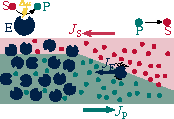
\includegraphics[width=0.7\textwidth]{figures/cips_scheme.pdf}
    \caption{Processes leading to catalysis-induced phase separation (CIPS). 
		(a) Enzymes convert substrate into product by a fuelled catalytic reaction, while product turns into substrate spontaneously. (b) The catalyzed reaction creates gradients of substrate and product around enzyme-rich regions, which attract more enzymes when the off-diagonal transport coefficients coupling enzyme fluxes to product and substrate thermodynamic forces satisfy $\Dpe>\Dse$.}
    \label{fig:cips_scheme}
\end{figure}

\subsection{Numerical Simulation}

Numerical solution of the evolution equations (\ref{eq:2-evoE})--(\ref{eq:2-evoP}) confirms the existence of this instability. We choose $\phie^*$ and solve for the steady state volume fractions of the other two components, $\phis^*$ and $\phip^*$, using equations (\ref{eq:2-sstar}) and (\ref{eq:2-pstar}). We initialize a 1D system with 200 grid points with volume fraction $\phie(x) = \phie^* + \delta_{\phi}(x)$ where at every grid point, $\delta_{\phi}(x)$ is drawn from a uniform distribution between $-0.005$ and $0.005$, to simulate Gaussian noise. The initial substrate and product concentrations are given by $\phi_i(x) = \phi_i^* - \phi_i^*\delta_{\phi}(x)/(\phi_S^*+\phi_P^*)$, which enforces constant volume everywhere.

Figure \ref{fig:CIPSnumeric} shows the spontaneous formation of regions of high and low enzyme concentrations when the system is unstable. Initially the large wavenumber, short length modes decay due to diffusive fluxes and following this longer wavelength modes are excited. Non-linear effects disrupt the growth of the Fourier modes and the system forms dense regions high in enzyme and dilute regions low in enzyme. These regions coarsen over time, ultimately resulting in two distinct phase-separated domains. Moreover, repeating this simulation with the same parameters but varying the amount of enzyme in the system, $\phie^*$, only changes the relative size of the high and low concentration domains, without affecting the concentration values in the two domains. This observation suggests the existence of a binodal line, as in equilibrium phase separation. This behaviour can be observed for all parameters which we simulated ($\kcat/\kspo\approx 1 \text{--} 100$, $\ve/\vs\approx 2 \text{--} 100$, $-\Delta \varepsilon\approx 5 \text{--} 30 k_{\rm B} T$, $\Delta \mu\approx5 \text{--} 50k_{\rm B} T$,  $\Dpe/\Dse\approx1 \text{--} 100$). The observation of macroscopic phase separation, rather than pattern formation or microphase separation, is further supported by the linear stability analysis showing an instability at the largest wavelengths ($q^2 \to 0$), rather than at finite wavelengths. Additional studies of two-component mass-conserving reaction-diffusion systems, have significant parallels to the minimal active model studied here and have shown coarsening leading to macrophase separation at long times \cite{brauns_phase-space_2020, brauns_wavelength_2021}.  A useful next step therefore is to try to predict the dilute and dense phases theoretically.
\begin{figure}
    \centering
    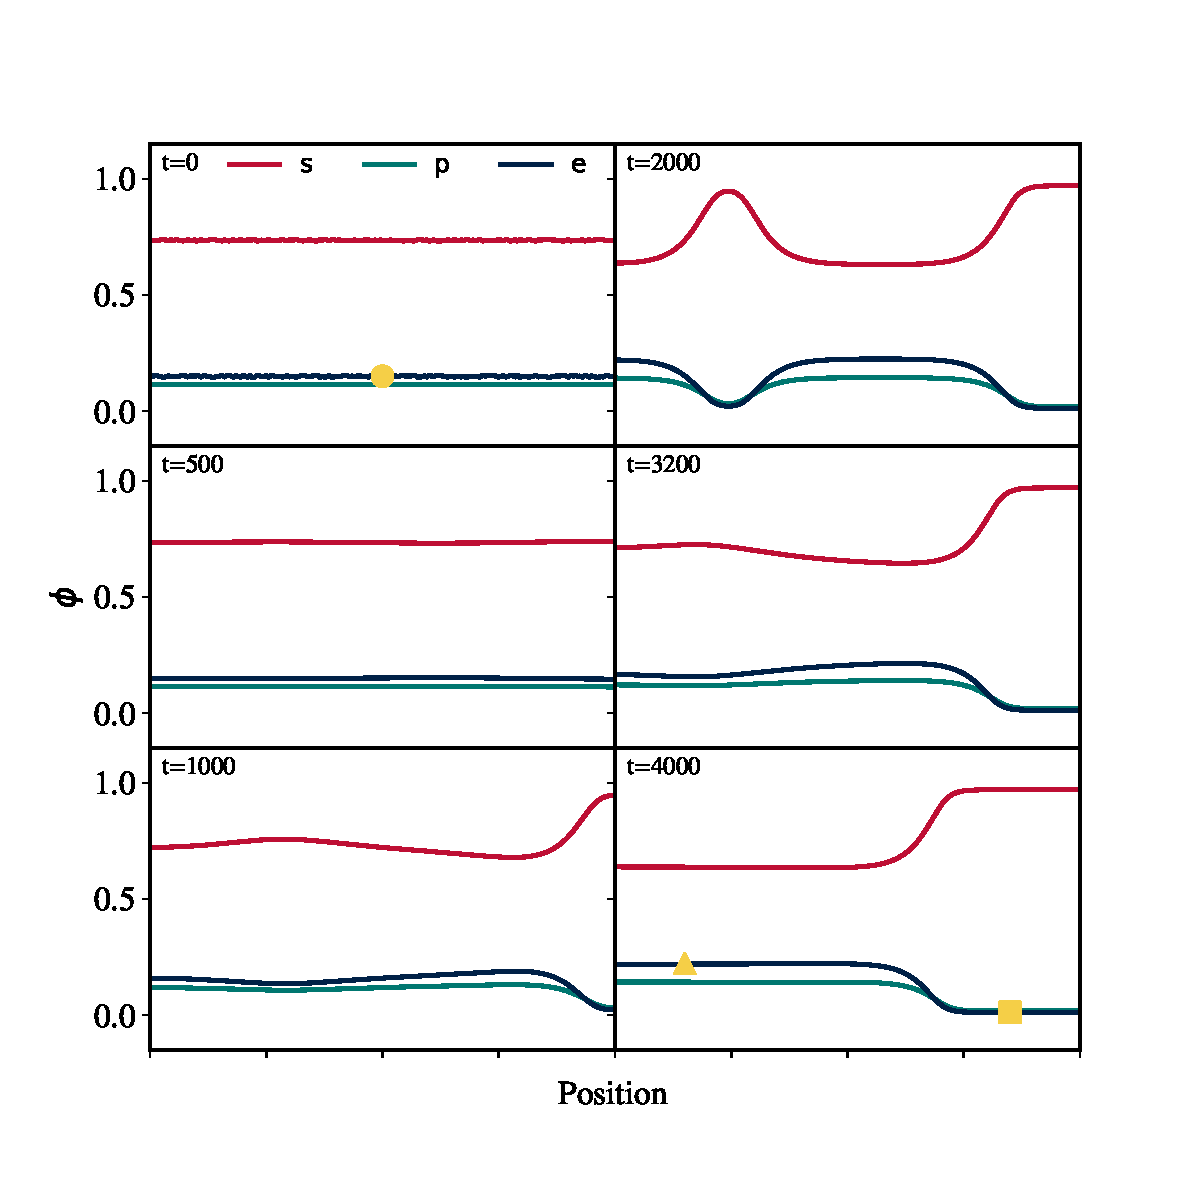
\includegraphics[width=\textwidth]{figures/CIPSnumeric.pdf}
    \caption{Numerical solution of an active mixture undergoing CIPS. The evolution of the system is shown at varying times, (non-dimensionalised by $\kspo$). The circle, triangle and square identify the homogeneous steady state and the dense and dilute enzyme phases, respectively, for comparison with figure \ref{fig:CIPSphase}. The system is initialised with a uniform steady state of $\phie=0.15$, $\phis=0.736$, and $\phip=0.114$, with $\Delta\mu=8 k_{\rm B} T$, $\kcat/\kspo=1$, $\Delta \varepsilon=-5 k_{\rm B} T$, $\Dpe=4 \Dse$, and $\Dps=10 \Dse$.}
    \label{fig:CIPSnumeric}
\end{figure}

\subsection{Effective free energy and Binodal}

In the macroscopic limit, we expect the substrate-product equilibrium in the bulk of each phase to be governed by the reaction terms that act locally, rather than by spatial diffusion. This implies that the substrate and product concentrations are enslaved to the enzyme concentration by $\phis \approx \phis^*(\phie)$ and $\phip \approx \phip^*(\phie)$, with the functions defined in (\ref{eq:2-sstar}) and (\ref{eq:2-pstar}). The system and its dynamics can now be described entirely as a function of the enzyme volume fraction $\phie$. All volume fractions, chemical potentials and mobilities describing the system are enslaved to $\phie$. As such equation (\ref{eq:2-evoE}) now becomes
\begin{equation}
    \dot{\phie} = \bm{\nabla} \cdot \left(\left(\Mee\frac{\mathrm{d}\mue}{\mathrm{d}\phie} + \Mes\frac{\mathrm{d}\mus}{\mathrm{d}\phie} + \Mep\frac{\mathrm{d}\mup}{\mathrm{d}\phie}\right)\bm{\nabla}\phie\right)
\end{equation}
We can recast the dynamics of the enzyme as $\dot{\phie}\approx \bm{\nabla} \cdot (\Mee\bm{\nabla}\mu_\mathrm{eff})$ with an effective chemical potential for the enzyme that satisfies
\begin{equation}
    \bm{\nabla}\mu_\mathrm{eff} = \left(\frac{\text{d}\mue}{\text{d}\phie} + \frac{\Mes}{\Mee}\frac{\text{d}\mus}{\text{d}\phie} + \frac{\Mep}{\Mee}\frac{\text{d}\mup}{\text{d}\phie}\right)\bm{\nabla}\phie.
\end{equation}
This means that by direct integration of the term in brackets with respect to $\phie$ we can calculate an effective chemical potential for the limit of fast reactions in the system. For the minimal model used here this integral can be evaluated exactly to give
\begin{equation}
    \frac{\mu_\mathrm{eff}(\phie)}{k_{\rm B} T} =  \log \phie - \frac{\ve}{\vs} \log[\Dse \phis^* (\phie) + \Dpe \phip^*(\phie)].
\end{equation}
We can also identify an effective free energy density $f_\mathrm{eff}(\phie)$, such that $\mu_\mathrm{eff}=\ve\frac{\mathrm{d} f_\mathrm{eff}}{\mathrm{d} \phie}$, which can be explicitly calculated by direct integration to give
\begin{equation}
\begin{split}
    \frac{f_\mathrm{eff}(\phie)}{k_{\rm B} T} &= \frac{1}{\vp}\frac{\kspo}{\kcat}\Bigg(\frac{1+e^{\beta \Delta \varepsilon}}{1+e^{-\beta (\Delta \varepsilon + \Delta \mu)}}\log\left[\frac{\kcat}{\kspo}\phie + e^{\beta (\Delta \varepsilon + \Delta \mu)}(1+e^{\beta \Delta \varepsilon} + \frac{\kcat}{\kspo}\phie)\right] \\
    -& \frac{\Dse+\Dpe e^{\beta \Delta \varepsilon}}{\Dpe+\Dse e^{-\beta (\Delta \varepsilon + \Delta \mu)}}\log\Big[\Dse\frac{\kcat}{\kspo}\phie + e^{\beta (\Delta \varepsilon + \Delta \mu)}(\Dse+\Dpe e^{\beta \Delta \varepsilon} + \Dpe \frac{\kcat}{\kspo}\phie)\Big]\Bigg) \\
    +&\left(\frac{1}{\vp}-\frac{1}{\ve}\right)\phie + \frac{1}{\vp}\log[1-\phie] + \phie\bigg(\frac{1}{\ve}\log\phie - \frac{1}{\vp} \log[\Dse\phis^*(\phie)+\Dpe\phip^*(\phie)]\bigg).
\end{split}
\end{equation}

Since $\mu_\mathrm{eff}$ can be determined up to a constant term, $f_\mathrm{eff}$ can be determined up to addition of an affine function in $\phie$. The effective dynamics $\dot{\phie}\approx \bm{\nabla} \cdot (\Mee\bm{\nabla}\mu_\mathrm{eff})$, with $\mu_\mathrm{eff}=\ve f'_\mathrm{eff}(\phie)$, drive the system towards a state that minimises the total effective free energy, under the constraints that the amount of enzyme and the volume of the system are conserved. Consequently, if the effective free energy is a good description of the system, the two phases the system forms should be predicted using the common tangent construction on the effective free energy. Using numerical methods to calculate the common tangent points \cite{wolff_thermodynamic_2011, doi_soft_2013} the coexisting phases and hence binodal line could be constructed as the system parameters were varied.

Having obtained both the spinodal and binodal curves, we can construct the phase diagram for the minimal active mixture as shown in figure \ref{fig:CIPSphase}. The phase separation is driven by the enzymatic activity and so the relevant control parameters in the system are the catalytic rate, $\kcat$, and the strength of the non-equilibrium drive, $\Delta\mu$. As the the strength of the enzymatic activity is decreased, the spinodal line (calculated from equation (\ref{eq:2-inst}) ) meets the binodal at a critical point showing good agreement. Below this critical point, the non-equilibrium drive is not strong enough to overcome diffusive fluxes and cause the phase seapration. These results also agree with the numerics for the system, where initialising a system in the unstable region ended with two phases as predicted from the effective free energy. However, it is important to note that in reality we are dealing with a nonequilibrium system, and moreover the effective quantities above were only obtained in the limit of fast reactions. In particular, as in other nonequilibrium systems \cite{wittkowski_scalar_2014}, the thermodynamic pressure $p_\mathrm{eff}$ may not necessarily coincide with the mechanical pressure exerted by the system on the walls of its container.

\begin{figure}
    \centering
    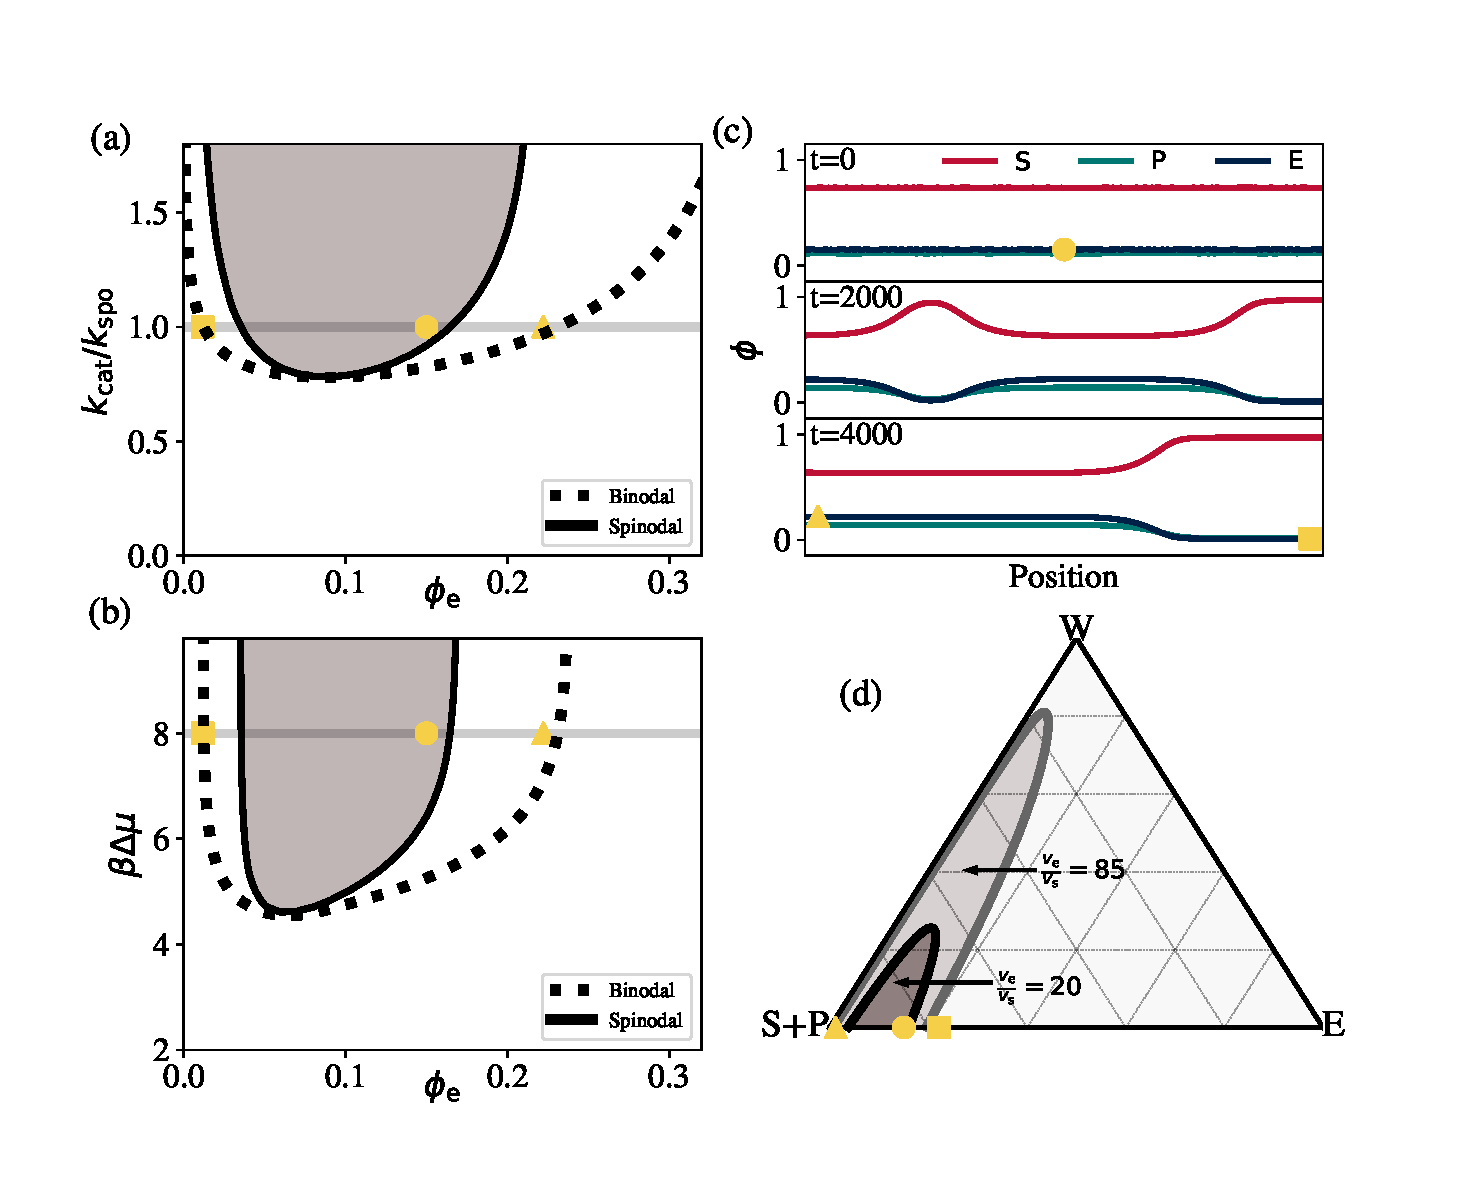
\includegraphics[width=\textwidth]{figures/CIPSphase.pdf}
    \caption{Phase behaviour and onset of CIPS. (a,b) Spinodal lines [from (\ref{eq:2-inst})] and binodal lines (from the common tangent construction of $f_\mathrm{eff}$) for (a) varying $\kcat$ with $\Delta\mu=8 k_{\rm B} T$ and (b) varying $\Delta \mu$ with $\kcat/\kspo=1$. (c) Numerical simulations showing the evolution of a uniform steady state with $\phie=0.15$ into two phase separated regions. The circle, triangle and square identify the homogeneous steady state and the dense and dilute enzyme phases, respectively, and are plotted in all other panels for comparison. (d) Stability diagram of a mixture including a water component, for $\Delta\mu=8 k_{\rm B} T$ and $\kcat/\kspo=1$. The darker and lighter shaded regions mark the spinodal regions for $\ve/\vs=20$ [also used in (a--c)] and $\ve/\vs=85$, respectively. Additional system parameters in (a--d) are $\Delta \varepsilon=-5 k_{\rm B} T$, $\Dpe=4 \Dse$, and $\Dps=10 \Dse$; in (d) $\Dew=\Dsw=\Dpw=10 \Dse$ and $\vw=\vs$.}
    \label{fig:CIPSphase}
\end{figure}

\subsection{Stability of a four-component system}

An additional solvent component (e.g. cholesterol in a lipid mixture) can be added to the system similarly to the enzyme component, with conserved dynamics and no reaction terms. We label this component $W$ with volume fraction $\phiw$. Following a similar procedure as for the no-solvent case, we can expand around a steady state where we now have $\phisp^* \neq 1 - \phie^*$ but $\phiw^* = 1 - \phisp^* - \phie^*$ where, similarly to the enzyme component, $\phiw^*$ is the average volume fraction of component W and is constant in the system. We can eliminate the solvent volume fraction to give a $3\times3$ matrix describing the evolution of the E, S, and P volume fractions
\begin{equation}
    (\dot{\delta\phie}, \dot{\delta\phis}, \dot{\delta\phip})^T = {\cal K}_{\rm w}(\delta\phie, \delta\phis, \delta\phip)^T    
\end{equation}
with
\newline
\noindent
\makebox[\textwidth]{\parbox{1.3\textwidth}{%
\begin{equation}
   {\cal K}_{\rm w} = 
\begin{tiny}
\begin{pmatrix}
(\Mse^*+\Mpe^*+\Mwe^*)\frac{\bm{q}^2}{\phie^*}+\Mwe^*\frac{\ve}{\vw}\frac{\bm{q}^2}{\phiw^*} & -\Mse^*\frac{\ve}{\vs}\frac{\bm{q}^2}{\phis^*}+\Mwe^*\frac{\ve}{\vw}\frac{\bm{q}^2}{\phiw^*} & -\Mpe^*\frac{\ve}{\vs}\frac{\bm{q}^2}{\phip^*}+\Mwe^*\frac{\ve}{\vw}\frac{\bm{q}^2}{\phiw^*}\\
-\Mse^*\frac{\bm{q}^2}{\phie^*}-\Ree +\Mws^*\frac{\vs}{\vw}\frac{\bm{q}^2}{\phiw^*} & (\Mse^*\frac{\ve}{\vs}+\Msp^*+\Mws^*)\frac{\bm{q}^2}{\phis^*}-\Rs  +\Mws^*\frac{\vs}{\vw}\frac{\bm{q}^2}{\phiw^*}& -\Msp^*\frac{\bm{q}^2}{\phip^*}+\Rp +\Mws^*\frac{\vs}{\vw}\frac{\bm{q}^2}{\phiw^*}\\
-\Mpe^*\frac{\bm{q}^2}{\phie^*}+\Ree +\Mwp^*\frac{\vs}{\vw}\frac{\bm{q}^2}{\phiw^*} & -\Msp^*\frac{\bm{q}^2}{\phis^*}+\Rs +\Mwp^*\frac{\vs}{\vw}\frac{\bm{q}^2}{\phiw^*} & (\Mpe^*\frac{\ve}{\vs}+\Msp^*+\Mwp^*)\frac{\bm{q}^2}{\phip^*}-\Rp +\Mwp^*\frac{\vs}{\vw}\frac{\bm{q}^2}{\phiw^*}\\
\end{pmatrix}
\end{tiny}
\end{equation}
}}

We now assume that the substrate and product dynamics are fast in comparison to the enzyme. Setting $\dot{\delta\phis}=\dot{\delta\phip}=0$ gives
\begin{equation}
    \dot{\delta\phie} = ({\cal K}_{\rm w}^{-1})_{1, 1}\delta\phie
\end{equation}
and so the system is unstable when
\begin{equation}
    ({\cal K}_{\rm w}^{-1})_{1, 1} = \frac{({\cal K}_{\rm w})_{2, 2}({\cal K}_{\rm w})_{3, 3}-({\cal K}_{\rm w})_{2, 3}({\cal K}_{\rm w})_{3, 2}}{\det({\cal K}_{\rm w})} \geq 0.
    \label{solvstab}
\end{equation}
The numerator of (\ref{solvstab}) is, to order $\bm{q}^2$,
\begin{equation}
    \bm{q}^2\Bigg[-\Rp \frac{\Mse^*\frac{\ve}{\vs}+\Mws^*}{\phis^*}-\Rs \frac{\Mpe^*\frac{\ve}{\vs}+\Mwp^*}{\phip^*}-\frac{\vs}{\vw\phiw^*}\big(\Rs +\Rp \big)\big(\Mws^*+\Mwp^*\big)\Bigg].
    \label{solvnum}
\end{equation}
With the common choice of mobilities, $M_{ij}<0$ for $i \neq j$, and $R_i \geq 0$, the expression (\ref{solvnum}) is positive and the instability condition is simply
\begin{equation}
    \det({\cal K}_{\rm w}) > 0,
\end{equation}
which marks the transition from having all negative eigenvalues to having two negative and one positive eigenvalue. The determinant of ${\cal{K}}_{\rm w}$ has many terms and even when truncated to order $\bm{q}^2$ it is not a manageable expression. Numerically evaluating this expression we find that in the low solvent limit ($\phiw \to 0$), and assuming Kramer's form for the mobilities, we recover the no-solvent case. Additionally, of we find that the uniform steady-state can be unstable even when all the solute components (enzyme, substrate, and product) are in dilute conditions, as shown in figure \ref{fig:CIPSphase}(d). This demonstrates the wide reach of this work and its potential application to realistic systems, where the components of the active minimal model may be part of a larger ensemble of molecules.

\subsection{Enzymatic Autoregulation}

A biologically pertinent question is what happens to the enzymatic activity when the system phase separates. The average rate of catalysis in a region of size $L$ is given by $\bar{r}_\mathrm{cat} = \frac{1}{L}\int_0^L r_\mathrm{cat} \mathrm{d}x$ in a simple 1D case. In a homogeneous state, $r_\mathrm{cat}$ will be constant throughout the system and, using equation (\ref{eq:2-r_cat}), will go as $\bar{r}_\mathrm{cat}^{\mathrm(h)}\sim\phie(1-\phie)$ which is a concave function of $\phie$. In a phase separated state, $\bar{r}_\mathrm{cat}$ is a weighted average of the catalytic rates in each phase, with the weights determined by the lever rule. Due to the concavity of $\rcat(\phie)$, we find that the catalytic rate in the phase separated state is always smaller than in the homogeneous state; $\rcat(\alpha\phie^{\mathrm{I}}+(1-\alpha)\phie^{\mathrm{II}}) \geq \alpha\rcat(\phie^{\mathrm{I}})+(1-\alpha)\rcat(\phie^{\mathrm{II}})$ shown graphically in figure~\ref{fig:CIPSautoregulation}(a). We observe a similar behaviour when we vary a control parameter such as $\Delta\mu$, which is controlled by the concentration of the fuel molecules in an experiment; see figure ~\ref{fig:CIPSautoregulation}(b). In the homogeneous phase, $\bar{r}_\mathrm{cat}$ initially rises and then saturates with increasing $\Delta\mu$. The phase separation reduces $\bar{r}_\mathrm{cat}$ in the whole system and leads to saturation at a lower activity. Through this mechanism, CIPS can act to autoregulate the enzymatic activity of the mixture: once the activity reaches a threshold, the system phase separates and gives rise to a reduced overall catalytic rate. A similar saturation effect is seen when other system parameters, such as $\kcat$, are varied causing the system to phase separate.

\begin{figure}
    \centering
    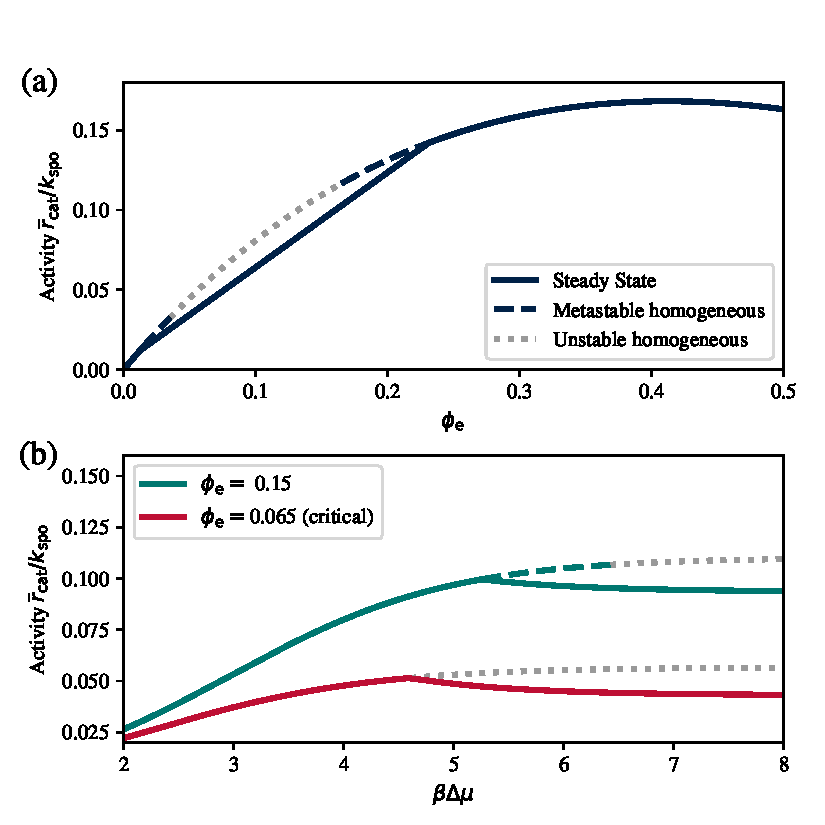
\includegraphics[width=0.8\textwidth]{figures/CIPSautoregulation.pdf}
    \caption{Effect of CIPS on catalytic activity. (a) Activity as a function of the initial $\phie$. In the phase separated state, the activity is a linear combination of the activity of the homogeneous states on either side of the binodal, which due to convexity is always smaller than that of the homogeneous state. (b) Evolution of activity with increasing $\Delta \mu$. As the system phase separates, the overall catalytic rate is reduced. When $\phie=0.065$, the system passes through the critical point and there is no metastable homogeneous branch. System parameters are $\Delta\mu=8 \kb T$, $\kcat/\kspo=1$, $\Delta \varepsilon=-5 \kb T$, $\Dpe=4 \Dse$, and $\Dps=10 \Dse$.}
    \label{fig:CIPSautoregulation}
\end{figure}

\section{Discussion}

The minimal active model studied here provides a thermodynamically-consistent description of a multicomponent fluid and identifies a new, purely non-equilibrium mechanism for phase separation as a consequence of the catalytic, fuelled conversion between two components (substrate and product) by a third component (enzyme). Alongside the fuelled catalytic reaction, this catalysis induced phase separation (CIPS), requires an asymmetry in the off diagonal mobility terms, which describe the strength of coupling between enzyme-substrate and enzyme-product thermodynamic forces and fluxes. An immediate question is therefore whether this asymmetry is present in real living systems, or, for synthetic systems, if it is hard to engineer this asymmetry.

At present, measurements of the off-diagonal Onsager mobilities for biologically relevant enzyme-substrate-product systems do not exist, however for a typical biological catalytic process, we expect both the spontaneous and catalyzed reactions to be strongly driven, and the enzyme protein to be much larger than the small molecular substrate and product. Given that the kinetics of catalyzed reactions are generally much faster than those of spontaneous ones (reduced energy barrier, with $\kcat\gg\kspo$), this implies that the threshold mobility asymmetry required for CIPS can become vanishingly small. A priori, there is no reason that the substrate and product will have symmetric response to gradients of the enzyme chemical potential and features of the molecular structure that may affect the coupling, such as shape or charge distribution will not be the same for different molecules. Existing experimental observations \cite{agudo-canalejo_phoresis_2018,zhang_chemically-powered_2021} of unequal response of enzymes to gradients of substrate and product suggest that an asymmetry may generically exist between the enzyme-substrate and enzyme-product Onsager mobilities. Furthermore, alternative descriptions of multicomponent diffusion, such as Fickian cross-diffusion \cite{vanag_cross-diffusion_2009} and Maxwell-Stefan diffusion \cite{taylor_multicomponent_1993} are equivalent to the Onsager framework and both molecular dynamics simulations and experimental measurements of these systems exhibit asymmetric responses \cite{guevara-carrion_mutual_2016, guevara-carrion_interplay_2018} and can drive pattern formation in membranes \cite{ramm_diffusiophoretic_2021}.

The mechanism behind CIPS is reminiscent of mechanisms for chemotactic or phoretic aggregation, where species move directly in response to gradients in other species \cite{keller_initiation_1970, golestanian_phoretic_2019} and can cause active components to self organise, such as interacting microorganisms or catalytic colloids \cite{saha_clusters_2014,agudo-canalejo_active_2019}. However, these studies were based on microscopic descriptions of the chemotactic or phoretic response, typically valid only under dilute conditions, whereas using the framework developed here keeps all components on equal footing as is valid for systems at arbitrary densities. This is particularly relevant to lipid membrane systems with high lipid compositions that could act as components of the minimal model.

Due to the catalytic conversion, CIPS is fundamentally non-equilibrium and results in phase separated states with non-vanishing fluxes, distinct from equilibrium mechanisms for phase separation. The latter rely on the presence of interaction terms (e.g.~$\chi_{ij}\phi_i\phi_j$ and $\kappa_{ij}\bm{\nabla} \phi_i \cdot \bm{\nabla} \phi_j$) in the free energy density $f_\mathrm{FH}$. Despite also requiring a size difference between components, CIPS is distinct from the entropic phase separation induced by depletion effects that is observed in binary hard-core mixtures \cite{frenkel_phase_1992}, which results in equilibrium phase separated states with vanishing fluxes. Future work may explore the competition or cooperation between equilibrium interactions and non-equilibrium catalytic effective interactions in phase separation. In particular, here we focused on effective interactions that are attractive, i.e.~those with $(1-e^{-\beta \Delta \mu})(\Dpe-\Dse)>0$ so that the right hand side of (\ref{eq:2-inst}) is positive. One may also consider repulsive effective interactions, with $(1-e^{-\beta \Delta \mu})(\Dpe-\Dse)<0$. In this case, we expect that an enzyme-rich condensate held together by equilibrium interactions may be {\it dissolved} by sufficiently strong non-equilibrium catalytic activity.

Another extension is to consider multi-step metabolic pathways, where the production of intermediate metabolites is known to regulate other reactions in the network and thus act as a feedback mechanism that inhibits overall metabolic activity \cite{oconnell_dynamic_2012,alam_self-inhibitory_2017}. CIPS provides a novel mechanism for this complex control of metabolism which, somewhat uniquely, autoregulates a single-step catalytic reaction and provides a simpler mechanism, potentially more amenable to fine-tuned synthetic control. A more complex reaction system with distinct enzymes, multiple species, or a different stoichiometry will change the regulatory effect of the phase separation. How this feedback could be used to control metabollic pathways is a relevant question. For example, CIPS may lead to colocalization of distinct enzymes within the same aggregate, allowing for substrate channelling as in cellular metabolons \cite{poshyvailo_does_2017, sweetlove_role_2018}.

\section{Outlook}

Membranes are full of chemically active enzymes that catalyse reactions \cite{alberts_molecular_2008} and it is important that models of membranes capture the effects of this activity. The minimal active mixture explored here is a prototypical example to demonstrate how catalysis can drive patterns in active mixtures such as membranes, and the simplicity of the model is exciting for engineering applications. The composition of membranes in living systems will of course be affected by other cellular processes, and even in model systems, geometry is likely to play a role in the dynamics of different components. For example, morphological changes in lipids \cite{phan_switchable_2023} and conformational changes in proteins, such as the enzymes would alter the membrane's local biophysical properties and through shape deformations could lead to another feedback mechanism \cite{seifert_bilayer-spanning_2015}. In addition to phase separation in the plane of a membrane, the theory developed here is independent to the number of spatial dimensions and CIPS may provide spatial organisation in the bulk of living cells.
\chapter{\label{ch:2-elastic}\chelastic} 

\minitoc

\section{Introduction}

Biological membranes are abundant and are crucial to cellular and sub-cellular organisation. Membranes allow for the spatial and temporal management of reactions and the separation of substances and environments \cite{simunovic_when_2015}. In addition to the familiar cellular membrane, eukaryotic cells also contain internal membranes that form the boundaries of organelles such as mitochondria, chloroplasts and lysosomes \cite{zimmerberg_how_2006}. Biological membranes are sheet-like lipid bilayers that are two molecules thick (4-10nm) \cite{berg_biochemistry_2002}. These are dynamic, fluid structures in which proteins float in a sea of lipids diffusing in the plane of the membrane and different composition of these proteins and lipids can generate asymmetry across the membrane. In addition to compartmentalisation, biological membranes serve several additional functions necessary for life, such as energy storage and information transduction, and many of these are dictated by the proteins associated with them.

Membranes are also a central focus in the development of novel biotechnology and biologically inspired materials. For example, surrounding substances with lipid bilayer membranes can create small compartments called liposomes that can aid in drug delivery \cite{lasic_applications_1995}. More recently, the development of DNA origami \cite{rothemund_folding_2006} has allowed for the engineering of sophisticated biomimetic systems of membranes that can control adsorption. These membranes are also candidates for controllable barriers, with engineered DNA nanopores displaying gating properties similar to natural ion channels and switch between open and closed states depending on the transmembrane voltage \cite{seifert_bilayer-spanning_2015}. Conventional engineered systems often rely on materials with specific properties at the atomic/molecular scale, but lack the hierarchical structure of interacting building blocks to enable macroscopic dynamic behaviour which is seen in biology \cite{studart_biologically_2015}. Tuneable and functional modules with active membranes may provide a scheme to develop these types of systems \cite{czogalla_dna_2016}. Additional to controlling the permeability of membranes, origami structures mimicking membrane-sculpting proteins have also been reported \cite{czogalla_amphipathic_2015} and present the possibility of controlling the shape of membrane bound compartments. Understanding more about the forces that govern the behaviour of membranes will therefore not only aid understanding of biophysical processes, but will also help to direct future bioengineering.

The shape of membranes is crucial to development and function. The endoplasmic reticulum (ER) and the Golgi apparatus have very complex boundaries defined by the curvature of the internal membrane, however they have distinctly different shapes. Both structures have very large surface area for their volume, however the ER is more tubular compared to the more saccular Golgi apparatus \cite{zimmerberg_how_2006}. This difference in structure may be related to the different functions of these organelles or as a consequence of the material within the organelle. Regardless, in order to understand the physical origin of these shapes, it is crucial to understand the interplay of the membrane with other biomolecules and structures and in particular the proteins embedded or tethered to the membrane. Membrane-bound proteins have been shown to be directly connected to membrane curvature and also to function, for example endocytosis being controlled by curvature inducing proteins that curve the membranes to form vesicles and allow the cell to take in external substances by engulfing the material \cite{boucrot_endophilin_2015}.

Different mechanisms can control the changes in membrane shape, for example transporter proteins that can generate forces by moving material across the membrane, or the cytoskeletal structure can pull on the membrane \cite{ghosh_pattern_2021}. These forces act to change the natural shape of the elastic membrane which  is stiff and resists shape changes away from a rest configuration. Deformations in the membrane shape can also be caused by a variety of curvature inducing inclusions, such as proteins that can bind to the membrane and insert structures that wedge the membrane and cause a bend \cite{simunovic_when_2015, argudo_continuum_2016}. Two or more of these inclusions can then interact elastically, as the membrane responds to a curvature that is locally imposed by each inclusions. Since these proteins are also able to move within the fluid membrane, they will respond to forces pulling them together or pushing them apart to minimise the energy of the global deformation.

The Bin/amphiphysin/Rvs (BAR) domain proteins are a common family of curvature inducing membrane proteins that have a curved domain and induce curvature on the membrane by binding to it. BAR proteins are involved in many cellular processes and they can both sense the curvature of the membrane and also influence the membrane shape. Different BAR domains have different shapes and this can cause different deformations in the membrane. One common feature across the BAR domains is that they are not rotationally symmetric and so the the proteins impose more complex constraints on the membrane than simple bowl like deformations. This anisotropy is essential to the formation of membrane tubules, as symmetric deformations imposed by bowl-like proteins, such as clathrin, form spherical vesicles instead \cite{simunovic_when_2015}. Thus, it is crucial to understand the elastic interactions between anisotropic proteins to gain insight into how membrane elasticity influences the cellular environment.

Prior work has studied the role of elastic interactions between membrane bound curvature inducing inclusions \cite{argudo_continuum_2016, helfrich_elastic_1973, kim_curvature-mediated_1998, brown_elastic_2008}. Different models assume different membrane tensions, inclusions separations and inclusion shape. One alternative to describing the distribution of individual interacting inclusions is to study the evolution of a density field that describes the distribution of curvature inducing inclusions on the surface of the membrane. Continuum models \cite{agudo-canalejo_pattern_2017} have been developed to study the stability of a uniform distribution of curvature inducing particles on a spherical vesicle. In addition to the elastic energy, the continuum framework is amenable to adding additional effects, such as the correlation of fluctuations, additional inclusion-inclusion interactions and even to couple the resulting deformations to the actomyosin cortex and other important cellular structures/processes \cite{ghosh_pattern_2021}. Growing instabilities in the distribution of curvature inducing inclusions may act to co-localise membrane proteins and to drive large scale shape changes in the cell \cite{garcia-lara_supramolecular_2015}.

However these top-down density field models do not specify any details of the mechanisms behind these interactions. This would be useful to know, to investigate specific regions of parameter space that correspond to the parameters observed in vivo. Understanding the mapping from individual particle properties to the parameters in the density description would present a new way to measure these small scale properties, provide alternative verification of current measurement techniques, or highlight broken symmetries from anisotropic curvature inducing inclusions. At very high densities of inclusions, interactions preventing inclusions from overlapping can drive the formation of a nematic phase \cite{tozzi_theory_2021}. However at lower densities, when the separation between these inclusions is large, the elastic interaction is less intuitive and the role of tension that resists deformations further complicates the interactions. This is the situation we study here, a system of interacting inclusions that are well separated embedded in a membrane with tension. This study is motivated by biological observations, however the results will also hopefully add another mechanism for the control of interactions of synthetic membranes and the formation of structures from individual inclusions.

\begin{figure}[h]
\centering
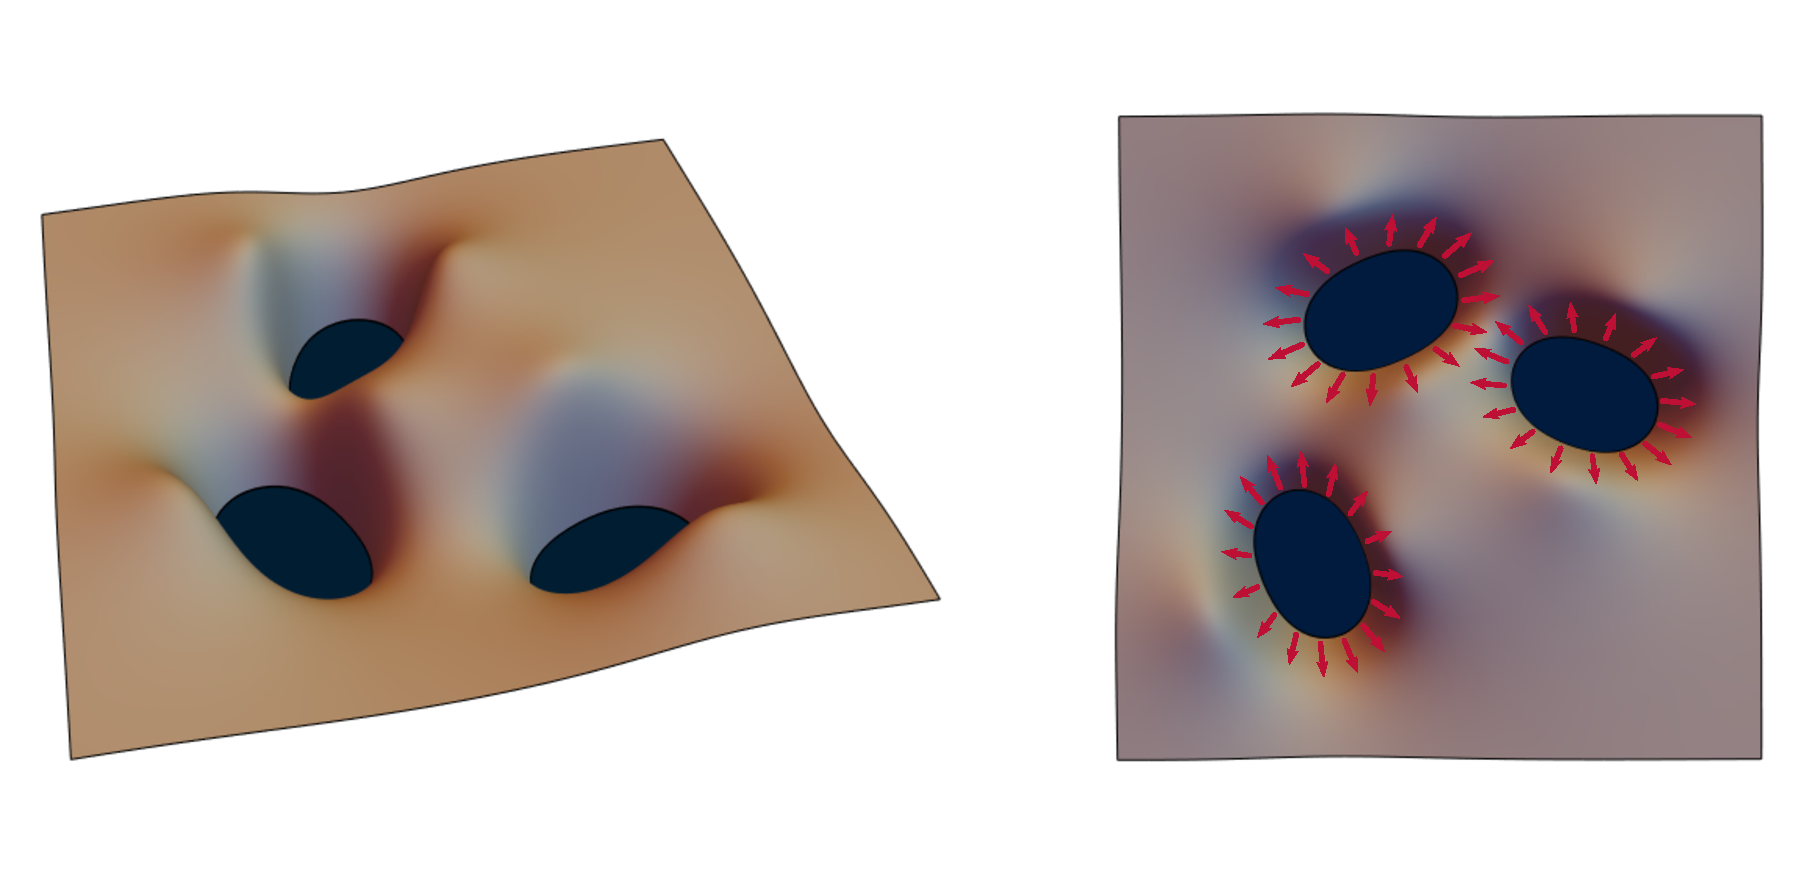
\includegraphics[width=12cm]{figures/3-elastic-figs/threeinc_scheme.pdf}
\caption{Example of three inclusions embedded in an elastic membrane and the resulting membrane shape from two different angles. The inclusions can interact via the elastic mediate membrane forces.}
\label{fig:overview}
\end{figure}

\subsection{Interactions of Anisotropic Inclusions}

Kwiecinski, Goriely and Chapman (KGC)\cite{kwiecinski_interactions_2020} described the interaction between two asymmetric inclusions by considering a circular inclusion that constrains the contact angle with the rest of the membrane, $\tilde{\alpha}$. The inclusions have radius $\epsilon$ and are typically separated by a distance $L$, such that $\epsilon \gg L$. Symmetric inclusions will have a constant contact angle, however in the anisotropic case the contact angle at the edge of the inclusion may vary and this gives the inclusions an orientation. The authors studied the case where the contact angle, $\tilde{\alpha}$, is
\begin{equation}
    \tilde{\alpha}=\tilde{\alpha}^{(0)} + \tilde{\alpha}^{(2)}_i\cos2\phi,
\end{equation}
and $\phi$ is the angular position on the edge of the inclusion (there is no term $\sim\cos\phi$ as this corresponds to tilting the membrane and does not contribute to any interaction energies). Surprisingly, breaking the symmetry of the inclusion results in an equilibrium separation between two interacting inclusions, where the interaction energy is locally minimised. This is a fundamentally different behaviour to the exclusively repulsive interactions seen by symmetric inclusions. Here we study a generalisation of this model to multiple interacting inclusions and study the effects of the broken symmetry and equilibrium inclusion separation.

\begin{figure}[h]
\centering
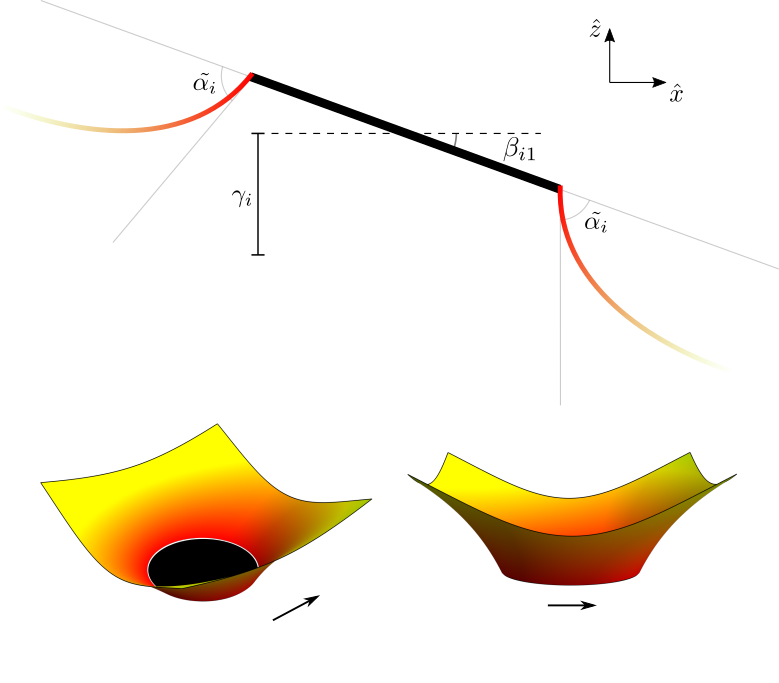
\includegraphics[width=12cm]{figures/3-elastic-figs/conttil.png}
\caption{Contact angle induced by a circular inclusion. The top scheme shows a cross section of the inclusion. The bottom two surface plots show the membrane response locally to an anisotropic inclusion, where the arrow indicates the orientation.}
\end{figure}

\section{Background}

\subsection{Helfrich Hamiltonian}

A common approach to describe the response of an elastic sheet to deformations is to use a Hamiltonian describing the energy of the membrane. The resulting physical system minimises this energy subject to the constraints of the bending \cite{deserno_fluid_nodate}. We can use the Helfrich Hamiltonian to calculate energy of a particular membrane geometry, described by the mean curvature $H$ and Gaussian curvature $K_G$. Additionally, the two monolayers in biological membranes can have different lipid composition and this can cause the rest configuration to no longer be flat and results in the bilayer having some non-zero intrinsic mean curvature, labelled $H_0$. This gives the energy of a membrane $E$ to be
\begin{equation}
    E = \int_{\Omega}\underbrace{\frac{\kappa}{2}(H-H_0)^2 + \overline{\kappa}K_G + T}_{\text{Helfrich Hamiltonian}}\text{d}A
    \label{helfrich}
\end{equation}
where $\kappa$ is the bending stiffness, $\overline{\kappa}$ is the saddle-splay modulus, $T$ is the tension and the integral is taken over the whole membrane, $\Omega$ \cite{kwiecinski_interactions_2020}. In this work, we consider $\Omega$ with fixed topology and with constant surface normal direction at the boundary of any inclusions. As such, the Gauss-Bonnet theorem gives the contribution from the Gaussian curvature, $K_G$, as only contributing a constant and thus not affecting the subsequent physics \cite{deserno_fluid_nodate}, unless there is a change in the membrane topology.

\subsection{Monge Parameterisation}

Cell membranes are much larger than curvature inducing inclusions (often these inclusions are simply proteins). Giant vesicles are used in many experiments on the physics of membranes and are smaller than cells, around \SI{20}{\micro\metre} in size,\cite{ramaswamy_nonequilibrium_2000} many times larger than the \SI{22}{\nano\metre} diameter of the abundant curvature inducing Bin/ amphiphysin/ Rvs (BAR) domain \cite{peter_bar_2004}. At the scale of the protein we therefore expect membranes to appear locally as planes with small regions of curvature induced by inclusions. As the proteins interact and potentially accumulate, or other cellular mechanisms force the membrane to curve this approximation may break down, but the assumption of a flat membrane provides a useful regime to explore the onset of these affects and allows us to use a Monge parameterisation to describe the surface \cite{deserno_fluid_nodate}. The Monge parameterization describes every point on a membrane $\textbf{r}=(x,y)$, as having height $\xi h(\textbf{r})$ above a reference plane (at $h=0$). Taking $\xi \ll 1$ this parameterisation describes surfaces that have small deformations and no overhangs. Additionally, we can nondimensionalize the position and the height by an arbitrary length, $L$. This choice allows us to write the mean curvature of the membrane, $H$, in terms of $h(\textbf{r})$ to give
\begin{equation}
    H = \nabla\cdot\Bigg(\frac{\nabla \xi h(\textbf{r})}{\sqrt{1+(\nabla \xi h(\textbf{r}))^2)}}\Bigg) = \xi \nabla^2h(\textbf{r}) + \mathcal{O}(\xi^2),
% \stackrel{\mathclap{\normalfont\mbox{|\nabla h| \ll 1}}}{\approx} t
\end{equation}
where the approximation is valid for $|\nabla h| \ll 1$. In this parameterisation, $\textbf{r}$ and $\nabla$ are defined as position and gradient operator of the base plane (i.e. $h=0$). As such, the area element is not simply $\text{d}A = \text{d}x\text{d}y$, but is given by
\begin{equation}
    \text{d}A = (1 + \xi^2|\nabla h|^2/2 + \mathcal{O}(\xi^4))\text{d}x\text{d}y .
\end{equation}
In a zero-temperature limit, the physical membrane will minimise the energy, $E$, in (\ref{helfrich}), which in this parameterisation is
\begin{equation}
    E= TA_0 + \xi^2\int_{\Omega}\left[\frac{\kappa}{2}(\nabla^2 h)^2 + \frac{T L^2}{2}|\nabla h|^2\right] \text{d}x\text{d}y + \mathcal{O}(\xi^3),
    \label{eq:efull}
\end{equation}
where $A_0$ is the area of the flat membrane. Considering a variation in $h(\textbf{r})$, i.e. $h(\textbf{r})\rightarrow h(\textbf{r})+\delta h(\textbf{r})$, the energy becomes to first order in $\delta h$
\begin{equation}
\begin{split}
    E[h(\textbf{r})+\delta h(\textbf{r})] = E[h(\textbf{r})] + 2\int \delta h (\nabla^4 h &- \mu^{-2}\nabla^2 h) \text{d}A \\
    &+ 2\oint\left(\nabla \delta h \nabla^2 h - \delta h \nabla^3 h + \mu^{-2} \delta h \nabla h \right) \cdot\textbf{n}\text{d}s = 0,
\end{split}
\label{eq:shape_eq}
\end{equation}
for a membrane with no spontaneous curvature ($H_0=0$). Equation (\ref{eq:efull}) is minimised when the membrane satisfies the shape equation
\begin{equation}
    \nabla^4 h - \mu^{-2}\nabla^2 h = 0,
    \label{eq:shape_eq}
\end{equation}
where $\mu=\sqrt{\kappa/TL^2}$. Additionally the boundary terms vanish, which imposes two further constraints on the boundary of the membrane. Either
\begin{equation}
    \oint\left(\nabla \delta h \nabla^2 h\right) \cdot\textbf{n}\text{d}s = 0,
    \label{eq:boundterm1}
\end{equation}
around the inclusion, impose the contact angle, which means that the term $\sim\nabla \delta h$ vanishes, or
\begin{equation}
    \oint\left(- \delta h \nabla^3 h + \mu^{-2} \delta h \nabla h \right) \cdot\textbf{n}\text{d}s = 0.
    \label{eq:boundterm2}
\end{equation}


Bending and deformations of the membrane are imposed by boundary conditions on $h$. For example the edge of a curvature-inducing inclusion will introduce an interior boundary with associated boundary conditions. In the bulk, the membrane then satisfies the shape equation subject to these constraints, and infinitely far away from the inclusion, the membrane returns to being flat. The perturbed membrane returns to being flat more slowly when tension is lower compared to the bending stiffness, but the membrane becomes flat more quickly in higher tension systems.

\section{One inclusion in an elastic membrane}
We begin by considering a single circular inclusion of radius $\tilde{d}=d \times L$ in an elastic sheet, where as before $L$ is the length scale used to non-dimensionalise the system. Through imposing a contact angle at its edge, the inclusion will induce a shape deformation in a flat membrane. Allowing the membrane to respond elastically, the membrane will adopt an equilibrium shape that minimises the energy subject to the imposed contact angle. To calculate this deformation we define a coordinate system, $(\tilde{x}, \tilde{y})$ with the origin the centre of the inclusion. Additionally we define a non-dimensional polar coordinate system such that $r=\sqrt{\tilde{x}^2 + \tilde{y}^2}/L$ and $\phi = \arctan(\tilde{y}, \tilde{x})$. In the scaled coordinate system the shape equation is as in Equation (\ref{eq:shape_eq}).

Far away from the inclusion, we impose the that the elastic sheet returns to the flat rest shape, so that
\begin{equation}
    \frac{\partial h}{\partial r} \biggr\rvert_{r\to\infty} = 0.
    \label{eq:flatfarfield}
\end{equation}
The contact angle $\tilde{\alpha}(\phi)$ defines the slope of the membrane at the edge of the inclusion relative to the plane of the inclusion. Note that since we non-dimensionalise both the membrane height and the coordinate system, $\tilde{\alpha}$ would be unchanged, however due to the additional scaling the contact angle differs by a factor of $\xi$ between the non-dimensional model and the dimensional system. The curvature-inducing inclusions are modelled as circular, however varying the contact angle around the edge of the inclusion gives the inclusions an orientation or shape more similar to studied biophysical structures. Since the contact angle must be continuous and periodic around the edge of the inclusion it can be expanded in Fourier modes as
\begin{equation}
\Tilde{\alpha}(\phi) = \sum_{m=0}^{\infty}\Tilde{\alpha}^{(m)}\cos(m\phi + \nu_{m}).
\end{equation}
We expect the lower order modes to induce the largest deformations and capture the distinct behaviours of curvature inducing inclusions. As such, we consider the first three modes of the expansion of the contact angle, when $m=0, 1, 2$, which we label the monopole, the dipole and the quadrupole modes, respectively. The dipole mode contributes to the contact angle with a positive contribution on one half of the inclusion a negative contribution on the other half and consequently generates a tilt in posture of the inclusion at equilibrium. The quadrupole and monopole modes do not generate a tilt, as the sign of the contact angle is symmetric about the diameters of the inclusion.

\subsection{Dipole Mode}
First, we consider an inclusion that imposes a contact angle with a dipole mode, $\propto \cos\phi$. When embedded in an elastic membrane, the inclusion will tilt to directly oppose the deformation of the membrane that the dipole boundary condition generates. This tilt alters the slope of the membrane at the inclusion edge (as the contact angle is now measured relative to the tilted inclusion) and it also changes the footprint of the inclusion, which will now appear as an ellipse in the $x-y$ plane. This makes the full, general problem of an inclusion with a dipole moment contact angle in an infinite sheet hard to solve. Instead, we consider the limit of the inclusion being small and the strength of the dipole moment being small resulting in a small tilt in the inclusion's posture which we describe by $\tan{\beta}$, so that the tilted inclusion makes an angle $\beta$ with the untitled position. The boundary is defined by the solution to 
\begin{equation}
    y^2 + \frac{x^2}{\cos\beta} = y^2 + x^2(1+\beta^2) = d^2
\end{equation}
where we have assumed the inclusion is orientated so that the tilt is about the $y$-axis. At linear order in $\beta$ the boundary of the inclusion is unchanged. The height on the edge of the inclusion will be $h(\rho=d, \theta)  = d \sin\beta \sin\theta \approx d \beta \sin\theta$ which for small inclusions, only contributes a correction to second order. The final modification from the tilt is the change in the membrane slope at the edge of the inclusion, which is
\begin{equation}
    \frac{\partial h}{\partial r}\bigg\rvert_{\partial\Omega} = \left(\Tilde{\alpha}^{(1)}+\beta\right)\cos(\phi).
\end{equation}

In this regime, the first order correction to the untitled inclusion only appears in the gradient of the membrane, similarly to a contact angle condition. Thus, for small $\Tilde{\alpha}^{(1)}$ the inclusion tilt will exactly match and cancel the dipole boundary condition. Inclusions with a dipole mode will therefore behave identically to inclusions without this term, but with a modified inclusion tilt. This will not affect the farfield membrane shape and subsequently will not affect the interactions between inclusions \cite{kwiecinski_interactions_2020}. Thus, we do not need to consider this mode in deriving the elastic interaction between inclusions and and we will not consider this effect further. \todo{Could do full calculation and take the limit. Need to ensure $\beta$ is sufficiently small (see BCs in matching).}
\notyet{
This gives the boundary conditions

Without loss of generality we can choose the axis of the tilt to be about the $y$-axis, as this is equivalent to rotating the inclusion. To keep the boundary conditions easier we redefine the $x-y$ plane so that the farfield membrane appears tilted and the inclusions lies flat, with a circular boundary. This gives the boundary conditions for the membrane shape as
\begin{equation}
\begin{split}
    \frac{\partial h}{\partial r}&\bigg\rvert_{r=d} = \Tilde{\alpha}^{(1)}\cos(\phi) \\
    h &\bigg\rvert_{r=d} = d\sin(\beta) = \beta +\mathcal{O}(\beta^2)
    \\
    \frac{\partial h}{\partial r} &\biggr\rvert_{r\to\infty} = 0.
\end{split}
\end{equation}
In this regime, we need to expand the shape equation about the reference state, which is now $h = \beta\cos\phi$.

In this regime, the projection of the boundary of the inclusion into the $x-y$ plane is unchanged to first order and thus the effect of a dipole contact angle is equivalent to tilting. When modelling multiple interacting inclusions, we will allow each inclusion to tilt and so including a dipole moment in the inclusion contact angle will act only to shift this tilt, but will not affect the interactions or energy of the system \cite{kwiecinski_interactions_2020}. We therefore will only consider inclusions without this contact angle contribution moving.



\todo{Therefore these fourier modes are the most simple contact angle modes that capture the three following types of inclusions: the monopole describes a radially symmetry curvature inducing inclusion, the dipole is the lowest order mode that breaks the symmetry, and the quadrupole is the lowest order mode that breaks the symmetry without inducing a tilt.}

\todo{Connect and link this to energy to bind a curved protein.}
\todo{Problem set up. And general, far field boundary conditons perhaps?}
\begin{equation}
\begin{split}
    \frac{\partial h}{\partial \hat{\mathbf{n}}_i}\bigg\rvert_{\partial D_i} = \left(\tilde\alpha_i(x,y) + \beta_{i1}\frac{\partial x}{\partial \hat{\mathbf{n}}_i} + \beta_{i2}\frac{\partial y}{\partial \hat{\mathbf{n}}_i}\right)
\end{split}
\end{equation}
where $\partial D_i$ is the edge of the inclusion.
\todo{we consider the first three modes and split them into modes that break induce a tilt and modes that do not}
The monopole and quadrupole modes are symmetric under reflections in $y=0$ and $x=0$ so that at equilibrium there is no tilt for a single inclusion embedded in a flat membrane. 
\todo{nuance around the rescaling of the membrane height/contact angle...}}
\subsection{Monopole and Quadrupole Modes}

The lowest order modes that do not induce a tilt for a single inclusion are the monopole and quadrupole modes, where the quadrupole mode breaks the radial symmetry and gives an inclusion an orientation. The monopole and quadrupole modes have strength $\Tilde{\alpha}^{(0)}$ and $\Tilde{\alpha}^{(2)}$ respectively so that the contact angle is
\begin{equation}
\Tilde{\alpha}(\phi) = \Tilde{\alpha}^{(0)} + \Tilde{\alpha}^{(2)}\cos(2\phi),
\end{equation}
as we can choose to set $\nu_0=\nu_2=0$ without loss of generality (this is simply choosing the orientation of the inclusion in the membrane). Despite not inducing a tilt, the monopole gives the inclusion a clear up and down orientation (a bowl looks different holding soup $\cup$ or trapping a spider $\cap$, face up or down) and so compared to the farfield flat membrane, we expect the inclusion to be positioned at some non-zero height, $\gamma$, that will depend on $\Tilde{\alpha}^{(0)}$. The boundary conditions for the membrane around the inclusion are therefore
\begin{equation}
\begin{split}
    \frac{\partial h}{\partial r}\bigg\rvert_{r=d} &= \Tilde{\alpha}^{(0)} + \Tilde{\alpha}^{(2)}\cos(2\phi) \\
    h \bigg\rvert_{r=d} &= \gamma.
\end{split}
\end{equation}
and $\gamma$ is determined by force balance on the edge of the inclusion. The general solution to the shape equation with a monopole and quadrupole is
\begin{equation}
\begin{split}
    h(r, \phi) &= A_{1}+A_{2}\log(r)+A_{3}I_{0}(r/\mu)+A_{4}K_{0}(r/\mu) \\
    &+ \cos(2\phi)\left(A_{5}r^2+\frac{A_{6}}{r^2}+A_{7}I_{2}(r/\mu)+A_{8}K_{2}(r/\mu)\right),
\end{split}
\end{equation}
where the $K_\nu$ are modified Bessel functions of the second kind. However, since the membrane must be flat as $r\to\infty$ we find $A_{3} = A_{5} = A_{7} = 0$ and imposing the boundary conditions at the inclusion boundary gives
\begin{equation}
    A_4 = -\frac{\Tilde{\alpha}^{(0)}\mu}{K_{1}(d/\mu)},\quad A_6 = \frac{\Tilde{\alpha}^{(2)} d^2 \mu K_{2}(d/\mu)}{K_{1}(d/\mu)},\quad A_8 = -\frac{\Tilde{\alpha}^{(2)} \mu}{K_{1}(d/\mu)}.
\end{equation}

At the boundary of the inclusion the normal derivative is fixed by the contact angle. Since the inclusion is rigid and not tilted $\delta h(\phi)$ is constant and the force balance becomes
\begin{equation}
    \oint_0^{2\pi}d\frac{\partial}{\partial \textbf{n}}\left(\nabla^2 h - \mu^{-2} h \right) \text{d}\phi = 0.
\end{equation}
Evaluating the integral for the membrane gives $A_{2} = 0$. The membrane shape is therefore
\begin{equation}
    h(r, \phi) = -\frac{\alpha^{(0)}\mu}{K_{1}(d/\mu)}K_{0}(r/\mu) + \cos(2\phi)\left(\frac{\alpha^{(2)} d^2 \mu K_{2}(d/\mu)}{ K_{1}(d/\mu)}r^{-2}-\frac{\alpha^{(2)}\mu
    }{K_{1}(d/\mu)}K_{2}(r/\mu)\right).
\end{equation}
The energy of the membrane can now be found by evaluating the energy functional in (\ref{eq:efull}) using the solution of the shape equation. A convenient way to calculate this is to integrate by parts, and evaluate the boundary terms. Using
\begin{equation}
    \int_{\Omega}\left((\nabla^2 h)^2 + \mu^{-2}|\nabla h|^2\right) \text{d}x\text{d}y = \int_{\partial\Omega}\left(\nabla^2 h\frac{\partial h}{\partial n} - h\frac{\partial}{\partial n}(\nabla^2 h) + \mu^{-2}h\frac{\partial h}{\partial n}\right) \text{d}s,
    \label{eq:eparts}
\end{equation}
% \begin{equation}
% \begin{split}
%     \int_{\Omega}\left((\nabla^2 h)^2 + \mu^{-2}|\nabla h|^2\right) \text{d}x\text{d}y &= \int_{\partial\Omega}\left(\nabla^2 h\frac{\partial h}{\partial n} - h\frac{\partial}{\partial n}(\nabla^2 h) + \mu^{-2}h\frac{\partial h}{\partial n}\right) \text{d}s \\
%      &= \int_{\phi=0}^{2\pi}\left(\nabla^2 h\frac{\partial h}{\partial n} - h\frac{\partial}{\partial n}(\nabla^2 h) + \mu^{-2}h\frac{\partial h}{\partial n}\right)d\text{d}\phi
%     \label{eq:eparts}
% \end{split}
% \end{equation}
gives the energy of the membrane to be
\begin{align}
    E &= TA_0 + \frac{L^2\xi^2\kappa}{2}\int_{0}^{2\pi}d\left(\nabla^2 h\frac{\partial h}{\partial n} - h\frac{\partial}{\partial n}(\nabla^2 h) + \mu^{-2}h\frac{\partial h}{\partial n}\right)\text{d}\phi, \\
    &= E_0 + E_{\text{def}}.
\end{align}
We evaluate the energy of the deformation, $E_{\text{def}}$, to be
\begin{equation}
\begin{split}
    \frac{2E_{\text{def}}}{L^2\xi^2\kappa} = \frac{2\pi\left(\alpha^{(0)}\right)^2 K_0\left(d/\mu\right)}{\mu K_1\left(d/\mu\right)} + \frac{2\pi\left(\alpha^{(2)}\right)^2}{4 d^3 \mu} &\Bigg[\frac{4d(d^2 + 2\mu^2)K_0\left(d/\mu\right)}{K_1\left(d/\mu\right)} + (9 d^2 \mu + 16\mu^3)\\
    &+ \frac{16\mu^3 K_2\left(d/\mu\right)^2}{K_1\left(d/\mu\right)^2} - \frac{d^2\mu K_3\left(d/\mu\right)^2}{K_1\left(d/\mu\right)^2}\Bigg].
\end{split}
\end{equation}

This result is exact for one inclusion in an infinite elastic membrane. However, for the small inclusions that induce membrane curvature we have that $d \ll 1$, where the choice of length scale gives $\mu\sim\mathcal{O}(1)$. The limiting behaviour of the modified Bessel functions for small arguments is $K_{0}(x) \sim -\ln(x/2)-\gamma$, where $\gamma$ is the Euler–Mascheroni constant and for $n > 0$ $K_{n}(x) \sim (2/x)^{n}\Gamma(n)/2$. The energy of the deformation to fourth order then becomes
\begin{equation}
    E = \frac{2\pi d^2 \left(\Tilde{\alpha}^{(0)}\right)^2}{\mu^2}\left( \gamma + \ln(d/2\mu) \right) + \frac{2\pi d^2 \left(\Tilde{\alpha}^{(2)}\right)^2}{\mu^2}\left(\frac{\mu^2}{d^2} + \gamma + \ln(d/2\mu) \right) + \mathcal{O}(d^4).
    \label{eq:SingleModQuad}
\end{equation}
\notyet{\todo{decide when we introduce the lenght scale. Else we need the boundary of the physical system to be $R\times L$ for example. Then $R$ can be small. Else need to compare $R$ and $\mu$.}}

\notyet{The linearisation of the  We will dsitinguish these two angles by with a tilde, so that a contact angle $\Tilde{\alpha}$ is the \textit{true} contact angle, which can be measured experimentally, but we also define a scaled contact angle $\alpha$, where we set $\Tilde{\alpha}=\epsilon\alpha$.... can we ?}
\notyet{
\subsection{Dipole Mode}

\begin{equation}
\begin{split}
    \frac{\partial h}{\partial \hat{\mathbf{n}}_i}\bigg\rvert_{\partial D_i} = \left(\tilde\alpha_i(x,y) + \beta_{i1}\frac{\partial x}{\partial \hat{\mathbf{n}}_i} + \beta_{i2}\frac{\partial y}{\partial \hat{\mathbf{n}}_i}\right)
\end{split}
\end{equation}
where $\partial D_i$ is the edge of the inclusion.


\todo{Comment about rotating the inclusion, but also this doesn't matter in the one inclusion case since the flat far field limit is the same everywhere.}

A circular inclusion in a membrane is described by the the radius of the inclusion and the contact angle it imposes on the surrounding membrane. The contact angle, $\alpha(\phi)$, imposed by an inclusion of radius $R$ can be expanded in Fourier modes such that $\alpha(\phi) = \sum_{m}\alpha^{(m)}\cos(m\phi)$. The lowest mode that breaks the symmetry of the inclusion goes like $\sim \cos\phi$ which we label the dipole mode. We start by considering an inclusion whose contact angle only contains this dipole mode, $\alpha(\phi) = \alpha^{(1)}\cos(\phi)$. The membrane is fixed in the farfield and the \textit{posture} of the inclusion (it's height and tilt) is determined by local force balance on the edge of the inclusion. However, since the contact angle is symmetric about the $y=0$, i.e. $\alpha(\phi) = \alpha(-\phi)$, the inclusion will not be titled about $y=0$. Instead, the inclusion will only be tilted about $x=0$ and we can describe this tilt by the angle the inclusion makes with the reference plane, $\beta$. The boundary conditions on the inclusion at the boundary are now
\begin{equation}
    h(\rho, \phi)|_{\partial \Omega} = \gamma + \alpha^{(1)}x = \gamma + \alpha^{(1)}\rho\cos\phi
\end{equation}
with the contact angle and tilt meaning that
\begin{equation}
    \nabla h|_{\partial \Omega} = (\beta + \alpha^{(1)})\hat{x} = =(\beta + \alpha^{(1)})(\cos\phi\hat{\rho}+\sin\phi\hat{\phi})
\end{equation}
where the inclusion boundary, $\partial\Omega$, is given by the solution to
\begin{equation}
    R^2 = x^2 + \frac{y^2}{cos^2\beta} = \rho^2\left(\sin^2\phi+\frac{\cos^2\phi}{\cos^2\beta}\right).
\end{equation}
in along that axis and so we can introduce a title parameter. An inclusion embedded in the membrane will be free to move in in all directions subject to forces from the membrane and thus for the dipole mode, we expect the inclusion to be tilted with respect to the reference plane. Boundary condition is the far field constant slope of $D$.

Lost track a bit, but the transform is as follows:
\begin{equation}
    \tan(\phi) = \tan(\tilde{\phi})\cos(\beta)
\end{equation}
\begin{equation}
    \rho = \tilde{\rho}\frac{\cos^2\beta+\cos^2\beta\tan^2\phi}{1+\cos^2\beta\tan^2\phi}
\end{equation}

 ofSince the inclusion is not fixed at the The inclusion will be free to tilt in, 

The general solution is

\begin{equation}
    h(\rho, \phi) = \cos(\phi)\left(A_{1}\rho + A_{2}\rho^{-1} + A_{3}I_{1}(\rho/\mu)+A_{4}K_{1}(\rho/\mu)\right)
\end{equation}
solution is with
\begin{equation}
    h(\rho, \phi) = \cos(\phi)\left(D\rho + R\left(-D R + \frac{(-2D + \alpha^{(1)})\mu K_{1}(R/\mu)}{K_{0}(R/\mu)}\right)\rho^{-1} + \frac{(2D-\alpha^{(1)})\mu}{K_{0}(R/\mu)} K_{1}(\rho/\mu)\right)
\end{equation}

leads to $D = \alpha^{(1)}/2$.}

\section{Multiple Inclusions in an Elastic Membrane}

When multiple inclusions are embedded in an elastic membrane, the resulting deformation field can be calculated in the same way. Each inclusion will constrain the value of the membrane and its derivatives on an interior boundary defined by the inclusion edge. Away from the inclusions the membrane returns to being flat. In general it is not possible to solve exactly for the shape of the membrane for an arbitrary configuration of inclusions. However, the small size of the inclusions can be exploited to determine a perturbation series for the membrane shape.

When the inclusions are small compared to the length scale of deformations, the deformation field around each inclusion will be dominated by the constraints from the contact angle of that specific inclusion. This defines an \textit{inner} region around each inclusion. When viewing the system on length scales comparable to the separation of inclusions, the membrane shape will be determined by all inclusions and this defines the \textit{outer} region. Studying the shape of the membrane in both regions and using matched asymptotic analysis give a perturbation series for the deformation field everywhere in response to the presence of all inclusions and so the interaction energy of the deformation due to the position and orientation of each inclusion can be calculated.

\subsection{Calculating the Membrane Shape}

We begin by considering a system containing $N$ inclusions which we parameterise as follows. The $i^{th}$ inclusion has its centre at $(x_i, y_i)$ and is a circular disc with a contact angle $\tilde{\alpha}_i$. The inclusion has a posture described by the height of the centre $\gamma_i$ and two angles $\beta_{i1}$ and $\beta_{i2}$ that describe the tilt about the $y$- and $x$-axis respectively. Even if the contact angle has no tilt inducing Fourier mode, the location of other inclusions could break the symmetry and generate tilts. Therefore on the boundary of the $i^{th}$ inclusion
\begin{equation}
    h\bigg\rvert_{\partial D_i} = \gamma_i + \beta_{i1}(x-x_i) + \beta_{i2}(y-y_i),
\end{equation}
where we have scaled the tilt and height by the small parameter $\xi$. The contact angle imposes
\begin{equation}
    \frac{\partial h}{\partial \hat{\mathbf{n}}_i}\bigg\rvert_{\partial D_i} = \tilde\alpha_i(x,y) + \beta_{i1}\frac{\partial x}{\partial \hat{\mathbf{n}}_i} + \beta_{i2}\frac{\partial y}{\partial \hat{\mathbf{n}}_i},
\end{equation}
where $\hat{\mathbf{n}}_i$ is the normal to the boundary in the $x-y$ plane. \notyet{Additionally, the force free... given by \todo{connect to previous single inc calcs}.}

Around each inclusion we define an inner coordinate system. The centre of each inclusion, $(x_i, y_i)$ is the origin for a set of local polar coordinates, $(\rho_i, \phi_i)$ where $\phi_i$ is measured from the $x$-axis. The inner radial coordinate is scaled by the inclusion radius, $\epsilon$, to give
\begin{equation}
    x-x_i = \epsilon \rho_i \cos\phi_i, \quad \text{and} \quad y-y_i = \epsilon \rho_i \sin\phi_i.
\end{equation}
We also define $\alpha_i$ as
\begin{equation}
    \alpha_i(\phi_i) = \epsilon\tilde\alpha_i(\phi_i) = \alpha_i^{(0)}+\alpha_i^{(2)}\cos(\phi_i + \psi_i)
\end{equation}
where the factor $\epsilon$ is equivalent to rescaling $h$. The anisotropy of the inclusion is defined as $\omega_i=\alpha_i^{(2)}/\alpha_i^{(0)}$ and we will consider the distinguished limit of strong anisotropy and strong tension: $\omega_i=\mathcal{O}(1)$ and $\mu=\mathcal{O}(1)$ as $\epsilon\rightarrow 0$. In this regime inclusion separations larger than the non-dimensionalised distance, $R > 1$, are tension dominated.
\begin{figure}[h]
\centering
% 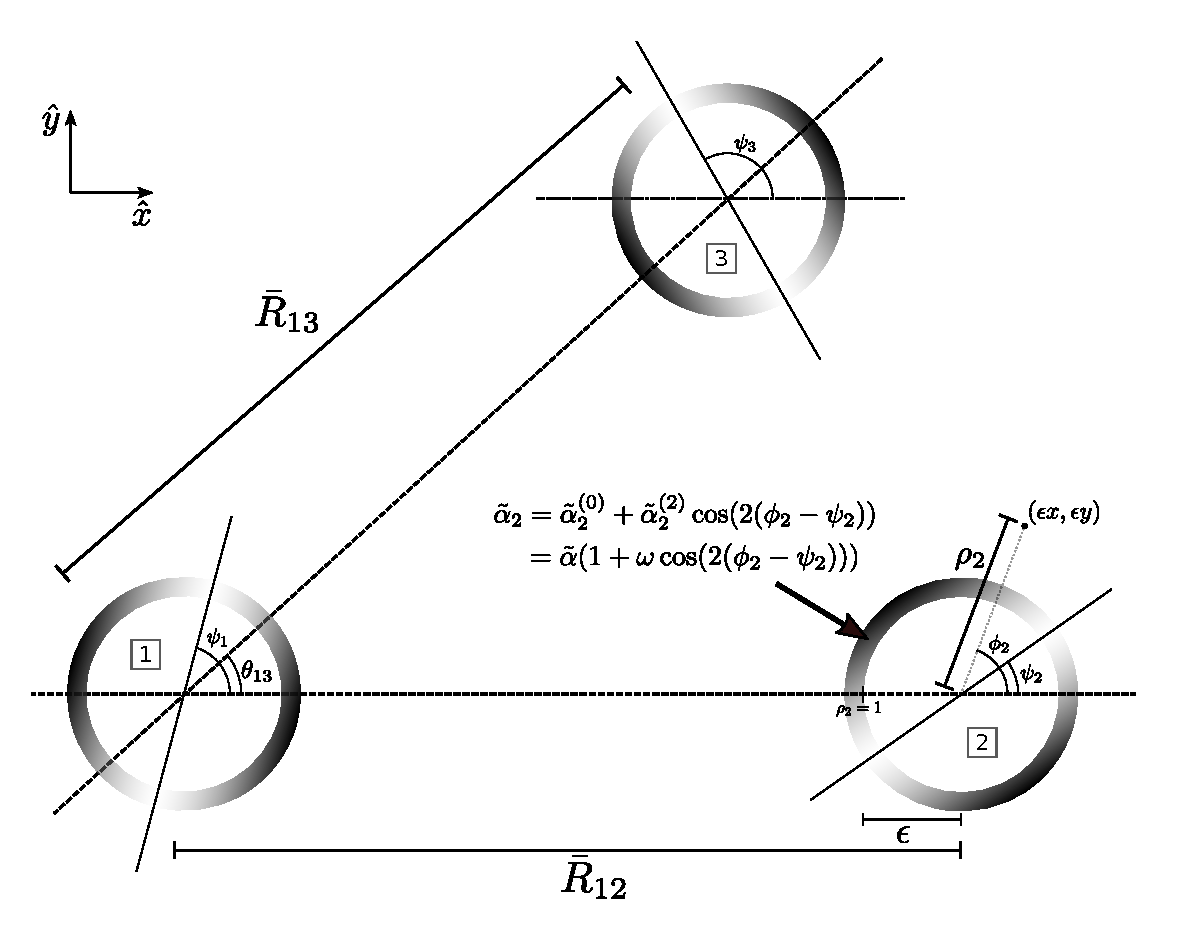
\includegraphics[width=12cm]{figures/3-elastic-figs/setup.pdf}
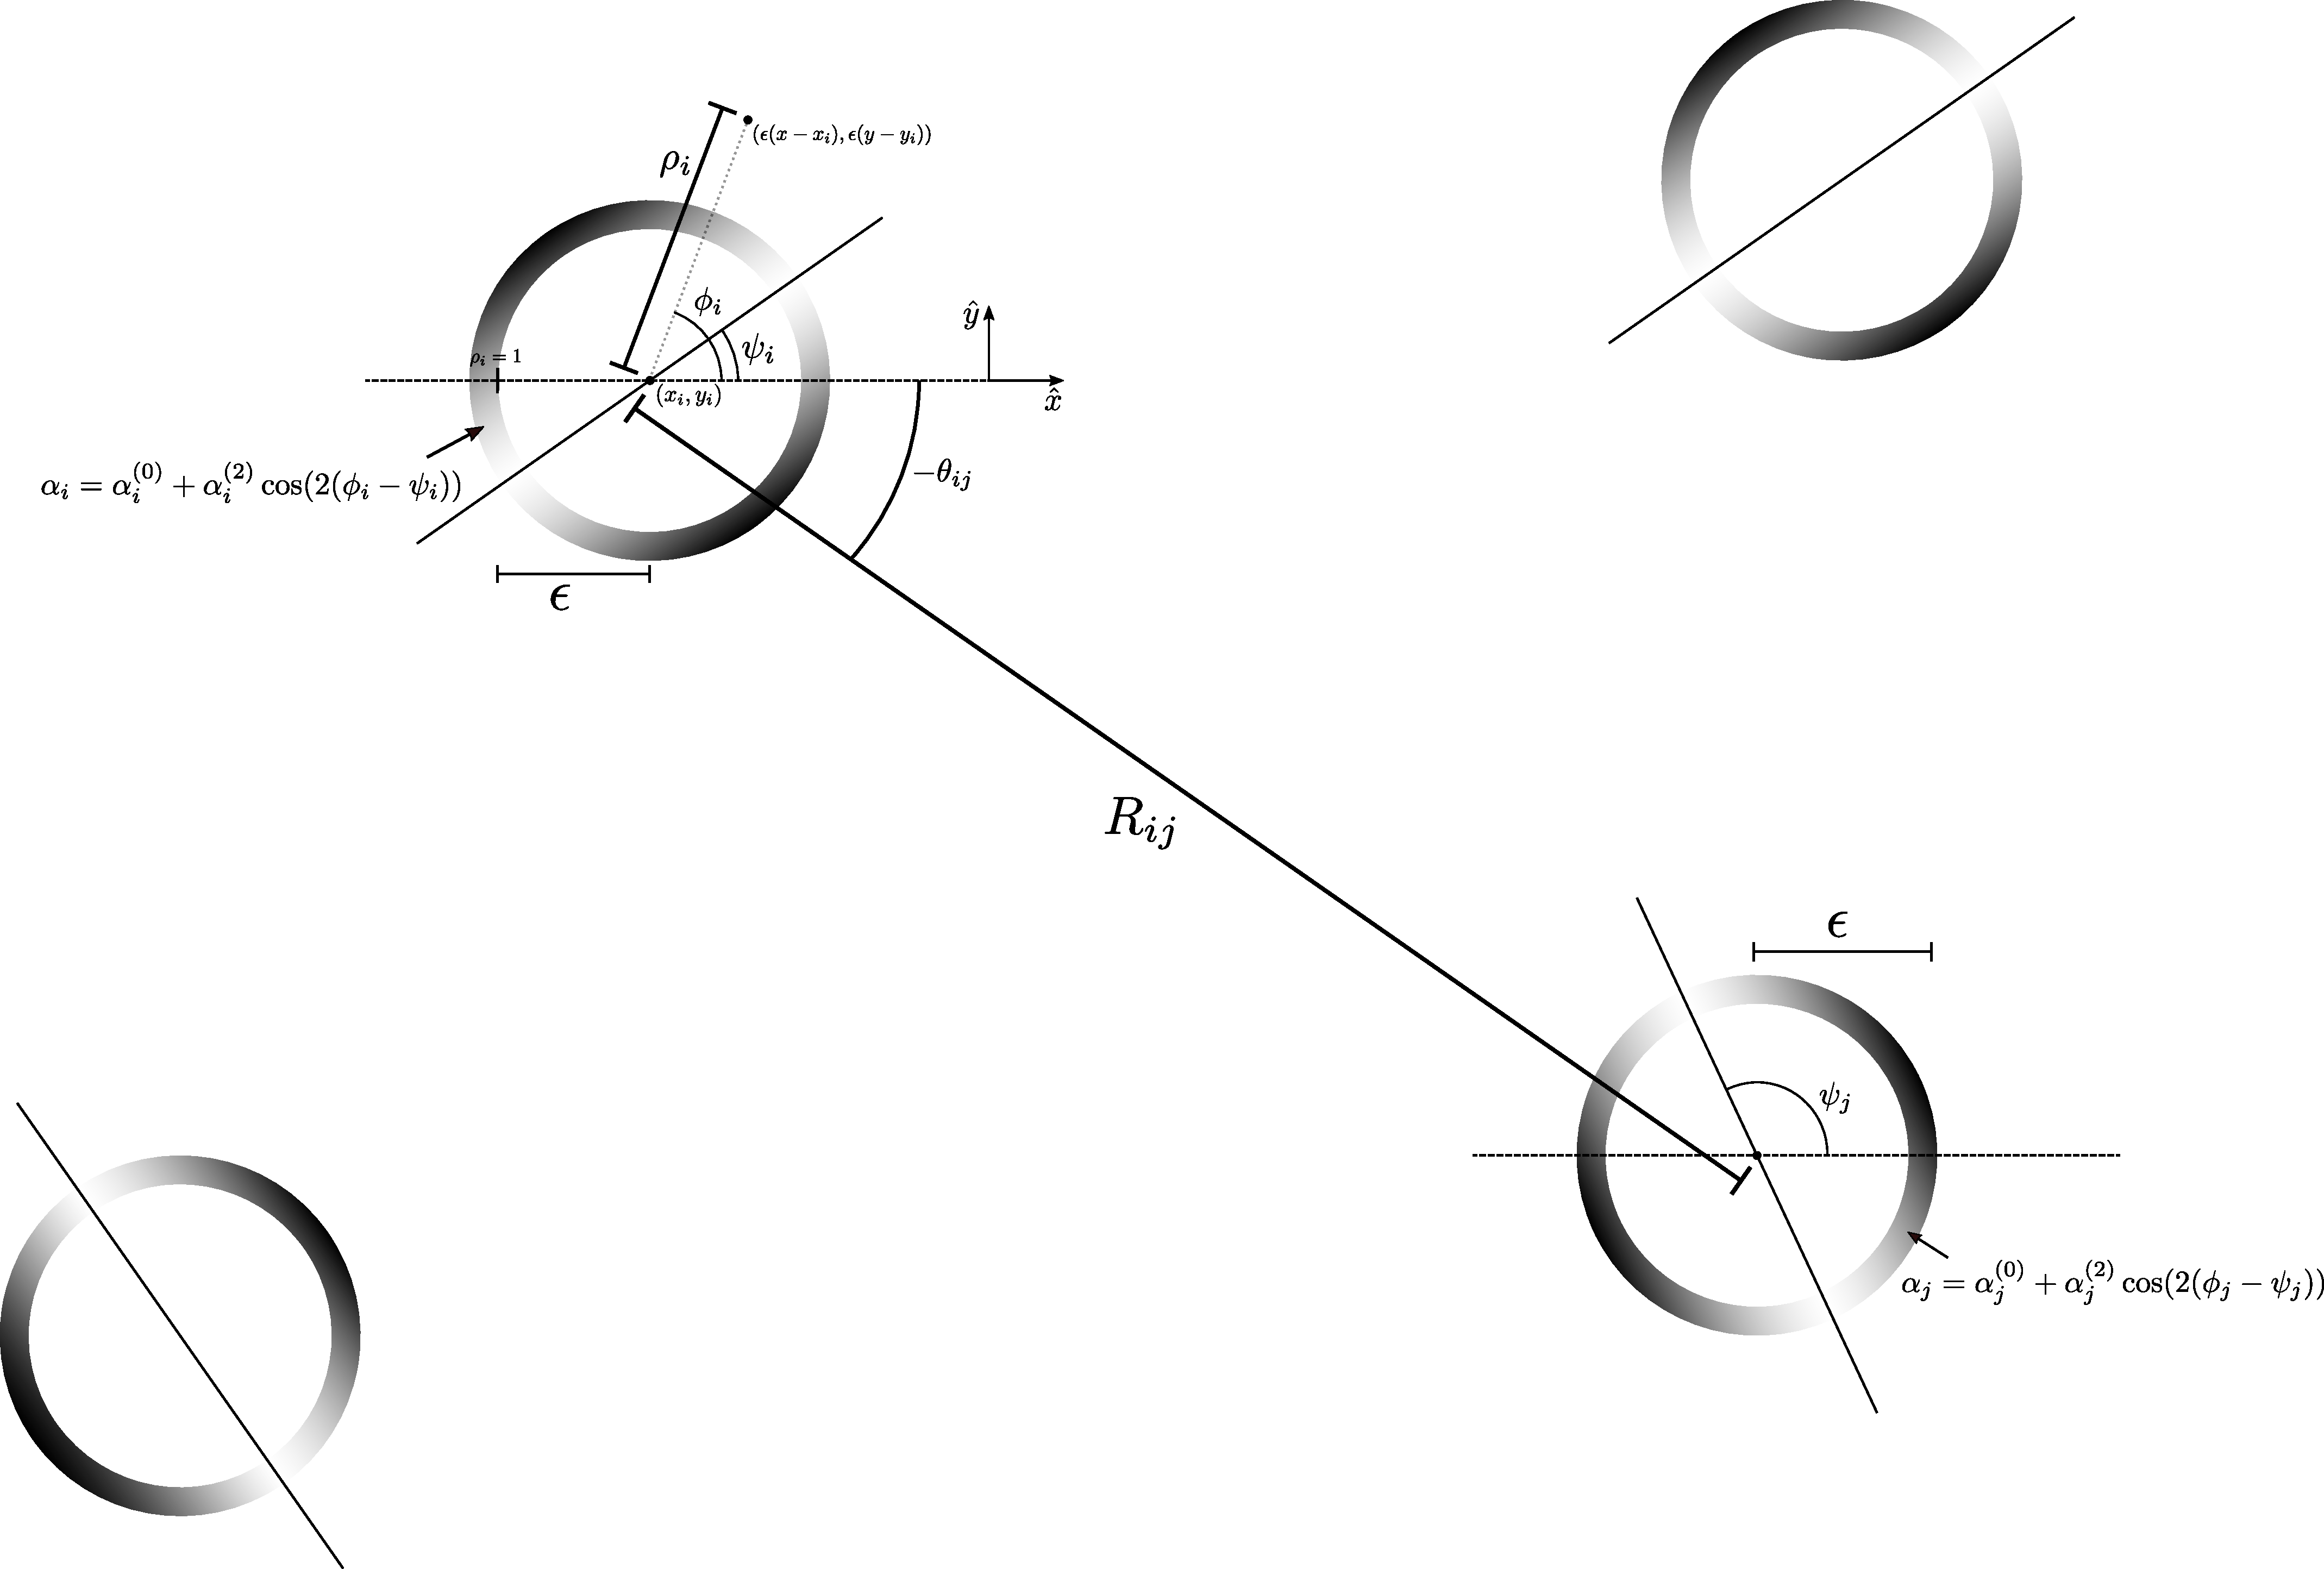
\includegraphics[width=12cm]{figures/3-elastic-figs/boundary_shade.pdf}
\caption{Parameterisation of the membrane elastic problem. The example shows the distribution of four inclusions where the inner coordinate system around the $i\text{th}$ inclusions is shown and the parameters describing the relative location of the $j\text{th}$ inlcusion are also shown. All angles are measured clockwise from the x-axis.}
\label{fig:setup}
\end{figure}

The inner region around the $i^{\text{th}}$ inclusion is described in local coordinates $(\rho_i, \phi_i)$, where the membrane height is $h_i(\rho_i, \phi_i)$ and the inclusion is a disc of radius 1. We expand the membrane height and the parameters describing the posture of the inclusion in the system in integer powers of $\epsilon$, for example, $h_i = h_i^{(0)}+\epsilon h_i^{(1)}+\epsilon^2 h_i^{(2)} + \cdots$ and $\beta_{i1} = \beta_{i1}^{(0)}+\epsilon \beta_{i1}^{(1)}+\epsilon^2 \beta_{i1}^{(2)} + \cdots$. In the inner coordinates, the shape equation (\ref{eq:shape_eq}) becomes
\begin{equation}
    \nabla^4_i h_i - \epsilon^2\mu^{-2}\nabla^{2}_i h_i = 0.
\end{equation}
where the subscript on the gradient operator indicates the coordinate system. This equation, along with the inclusion boundary conditions, must be satisfied at every order. The membrane shape in the outer region is given by $h_o(x, y)$, which we also expand in powers of $\epsilon$, and the inclusions appear as point singularities as $\epsilon\rightarrow0$.

\notyet{The inner region around the $i^{\text{th}}$ inclusion is described by the local coordinates $(\rho_i, \phi_i)$ and the membrane height in this region is $h_i(\rho_i, \phi_i)$ and the inclusion is a disc of radius $1$ in the inner coordinates. The membrane shape in the outer region is given by $h_o(x, y)$ and the inclusions appear as point singularities as $\epsilon\rightarrow0$. We expand the membrane height and parameters describing the posture of the inclusion in the system in integer powers of $\epsilon$, for example, $h_o = h_o^{(0)}+\epsilon h_o^{(1)}+\epsilon^2 h_o^{(2)} + \cdots$ and $\beta_{i1} = \beta_{i1}^{(0)}+\epsilon \beta_{i1}^{(1)}+\epsilon^2 \beta_{i1}^{(2)} + \cdots$. In the inner coordinates, the shape equation (\ref{eq:shape_eq}) becomes
\begin{equation}
    \nabla^4_i h_i - \epsilon^2\mu^{-2}\nabla^{2}_i h_i = 0.
\end{equation}
where the subscript on the gradient operator indicates the coordinate system. This equation, along with the inclusion boundary conditions, must be satisfied at every order.}

\notyet{\todo{need to have in here about the boundary and the tilt being a first order correction due to the radius epsilon term no?}}

\subsection{Matching}
At leading order the inner solution must satisfy
\begin{align}
    &\nabla_i^{4}h_i^{(0)}=0,  \\
    &h_i^{(0)}\biggr\rvert_{\rho_i=1}=\gamma_i^{(0)}, \\
    &\frac{\partial h_i^{(0)}}{\partial \rho_i}\biggr\rvert_{\rho_i=1}=\alpha_i^{(0)}+\alpha_i^{(2)}\cos(2\phi_i-2\psi_i).
\end{align}
\notyet{\todo{and the appropriate force balance conditions.}} In two-dimensional polar coordinates the biharmonic equation can be solved by separation of variables to obtain the so called  Michell solution. The boundary conditions only allow solutions with the monopole and quadrupole angular dependence, giving
\begin{equation}
    \begin{split}
    h_i^{(0)} &= \gamma_i^{(0)} + \alpha_i^{(0)}\log\rho_i + \frac{\alpha_i^{(2)}\cos 2\psi_i}{2}\cos 2\phi_i + \frac{\alpha_i^{(2)}\sin 2\psi_i}{2}\sin 2\phi_i \\
    &-\frac{\alpha_i^{(2)}\cos 2\psi_i}{2}\frac{\cos 2\phi_i}{\rho_i^2} - \frac{\alpha_i^{(2)}\sin 2\psi_i}{2}\frac{\sin 2\phi_i}{\rho_i^2}.
    \end{split}
\end{equation}
In the outer region, the shape equation for $h_o$ is the same at every order. For example, the leading order is
\begin{equation}
    \nabla^{4}h_o^{(0)}-\mu^{-2}\nabla^{2}h_o^{(0)}=0.  
\end{equation}
Around each inclusion the membrane approaches a singularity, which must match with the inner solution. This solution that matches and decays at infinity is given by
\begin{equation}
    h_o^{(0)} = c_0 + \sum_i \left( c_{1i} K_0(r_i/\mu) + c_{2i} \cos(2\phi_i-2\psi_i)\left(\frac{4\mu^{2}}{r_i^2} - 2 K_2(r_i/\mu)\right) \right),
\end{equation}
where $r_i = ((x_ - x_i)^2+(y - y_i)^2)^{1/2}$ and $\phi_i = \tan^{-1}((y - y_i)/(x - x_i))$. Expanding in inner variables about inclusion $i$ gives
\begin{alignat}{2}
        h_o^{(0)} &= c_0\; - &&c_{1i}(\gamma + \log(\epsilon\rho_{i}/2\mu))+\frac{c_{1i}}{4}(1-\gamma + \log 2 - \log \epsilon\rho_{i}/\mu)\frac{\epsilon^2 \rho_{i}^2}{\mu^2} \notag\\
        &+ c_{2i}\cos&&(2\phi_i-2\psi_i)\left( 1 + \frac{\epsilon^2\rho_{i}^2\log(\epsilon\rho_{i}/2\mu)}{4\mu^2} + \frac{\epsilon^2\rho_{i}^2(4\gamma - 3)}{16\mu^2}\right)\notag\\
        &+\mathlarger{\mathlarger{\sum}}_{j\neq i}&&\Bigg\{c_{1j}\Bigg[K_0\left(\frac{R_{ij}}{\mu}\right) + \frac{K_1\left(\frac{R_{ij}}{\mu}\right)}{\mu}\epsilon\rho_{i}\cos(\phi_i-\theta_{ij}) + \frac{K_0\left(\frac{R_{ij}}{\mu}\right)}{{2\mu^2}}\epsilon^2\rho_{i}^2\cos^2(\phi_i-\theta_{ij})\notag\\
        & &&+ \frac{K_1\left(\frac{R_{ij}}{\mu}\right)}{2\mu R_{ij}}\cos(2\phi_i-2\theta_{ij})\epsilon^2\rho_{i}^2\Bigg] \notag\\
        & &&+ c_{2j}\Bigg[\cos(2\psi_j-2\theta_{ij})\Bigg(f\left(\frac{R_{ij}}{\mu}\right) - \frac{\epsilon\rho_{i}\cos(\theta_{ij}-\phi_i)f'\left(\frac{R_{ij}}{\mu}\right)}{\mu} \notag\\
        & &&+ \epsilon^2\rho_{i}^2\bigg(-\frac{2f\left(\frac{R_{ij}}{\mu}\right)\sin^2(\phi_i-\theta_{ij})}{R_{ij}^2}+\frac{\sin^2(\phi_i-\theta_{ij})f'\left(\frac{R_{ij}}{\mu}\right)}{2\mu R_{ij}} + \frac{\cos^2(\phi_i-\theta_{ij})f''\left(\frac{R_{ij}}{\mu}\right)}{2\mu^2}\bigg)\Bigg)\notag\\
        & &&+ \sin(2\psi_j-2\theta_{ij})\Bigg(-\frac{2\epsilon\rho_{i} f\left(\frac{R_{ij}}{\mu}\right)\sin(\phi_i-\theta_{ij})}{R_{ij}} \notag\\
        & &&+ \epsilon^2\rho_{i}^2\bigg(-\frac{2\cos(\phi_i-\theta_{ij})f\left(\frac{R_{ij}}{\mu}\right)\sin(\phi_i-\theta_{ij})}{ R_{ij}^2} + \frac{2\cos(\phi_i-\theta_{ij})\sin(\phi_i-\theta_{ij})f'\left(\frac{R_{ij}}{\mu}\right)}{R_{ij}\mu}\bigg)\Bigg)\Bigg]\Bigg\} + O(\epsilon^3), %no \notag to number the equation
    \label{eq:leadingoutersecondinner}
\end{alignat}
which matches the leading order inner solutions to give
\begin{equation}
    c_{1i} = -\alpha_{i}^{0}, \quad c_{2i} = \frac{\alpha_{i}^{2}}{2},
\end{equation}
and
\begin{equation}
    \gamma_i^{(0)} = c_0 - c_{1i}\left(\log\frac{\epsilon}{2\mu}+\gamma\right) +\mathlarger{\sum}_{i\neq j}\left\{c_{1j}K_0(R_{ij}/\mu) +c_{2j}\cos(2\psi_j)\left(\frac{4\mu^2}{R_{ij}^2}- 2K_{2}(R_{ij}/\mu)\right)\right\}.
\end{equation}
At first order, the inner equation is
\begin{align}
    &\nabla_i^{4}h_i^{(1)}=0, \label{inner1order}\\ &h_i^{(1)}\biggr\rvert_{\rho_i=1}=\gamma_i^{(1)}+\beta^{(0)}_{i1}\cos(\phi_i)+\beta^{(0)}_{i2}\sin(\phi_i), \label{inner1orderBCval}\\
    &\frac{\partial h_i^{(1)}}{\partial \rho_i}\biggr\rvert_{\rho_i=1}=\beta^{(0)}_{i1}\cos(\phi_i)+\beta^{(0)}_{i2}\sin(\phi_i).\label{inner1orderBCderriv}
\end{align}
Additionally, as $\rho_1\to\infty$ the solution must match with the first order terms in equation (\ref{eq:leadingoutersecondinner}) and so 
\begin{equation}
\begin{split}
    h_i^{(1)}\biggr\rvert_{\rho_i\to\infty} \sim \mathlarger{\mathlarger{\sum}}_{j \neq i} \Bigg\{ &\rho_i \cos (\phi_i) \Bigg(\frac{c_{1j} \cos (\theta_{ij}) \left( K_1\left(\frac{R_{ij}}{\mu }\right) - c_{2j} \cos (2 \psi_j-2 \theta_{ij} ) f'\left(\frac{R_{ij}}{\mu }\right)\right)}{\mu}\\
    &+\frac{2 c_{2j} \sin (\theta_{ij} ) f\left(\frac{R_{ij}}{\mu }\right) \sin (2 \psi_j-2 \theta_{ij} )}{R_{ij}}\Bigg) \\
    &+\rho_i  \sin (\phi_i) \Bigg(\frac{\sin (\theta_{ij} ) \left(c_{1j} K_1\left(\frac{R_{ij}}{\mu }\right)-c_{2j} \cos (2 \psi_j-2 \theta_{ij} ) f'\left(\frac{R_{ij}}{\mu }\right)\right)}{\mu } \\
    &-\frac{2 c_{2j} \cos (\theta_{ij} ) f\left(\frac{R_{ij}}{\mu }\right) \sin (2 \psi_j-2 \theta_{ij} )}{R_{ij}}\Bigg)\Bigg\}.
\end{split}
\end{equation}
The solution to (\ref{inner1order}) with the correct limiting behaviour is
\begin{equation}
    h_i^{(1)} = \gamma_i^{(1)}+\beta^{(0)}_{i1} \rho_i \cos(\phi_i)+\beta^{(0)}_{i2} \rho_i \sin(\phi_i)
\end{equation}
where the matching gives
\begin{equation}
\begin{split}
    \beta^{(0)}_{i1} = \mathlarger{\sum}_{j \neq i}\; &\frac{c_{1j} K_1\left(\frac{R_{ij}}{\mu}\right)\cos (\theta_{ij})}{\mu}-\frac{c_{2j} \cos (2 \psi_j-2\theta_{ij})\cos (\theta_{ij}) f'\left(\frac{R_{ij}}{\mu }\right)}{\mu}\\
    &+\frac{2 c_{2j} \sin (\theta_{ij}) f\left(\frac{R_{ij}}{\mu }\right) \sin (2\psi_j-2 \theta_{ij})}{R_{ij}}, \\
    \beta^{(0)}_{i2} = \mathlarger{\sum}_{j \neq i}\; &\frac{c_{1j} K_1\left(\frac{R_{ij}}{\mu}\right)\sin (\theta_{ij})}{\mu}-\frac{c_{2j} \cos (2 \psi_j-2\theta_{ij})\sin (\theta_{ij}) f'\left(\frac{R_{ij}}{\mu }\right)}{\mu}\\
    &-\frac{2 c_{2j} \cos (\theta_{ij}) f\left(\frac{R_{ij}}{\mu }\right) \sin (2\psi_j-2 \theta_{ij})}{R_{ij}}.
\end{split}
\end{equation}
Note the difference of sign in the term $\sim \sin (2\psi_j-2 \theta_{ij})$ between $\beta^{(0)}_{i1}$ and $\beta^{(0)}_{i2}$.
\notyet{This is due to the symmetry of the This can be understood by considering a change of coordinate system, for example changing the sign of one axis (such that any angle $\sigma \rightarrow -\sigma$), or a by a rotation of $\pi/2$ ($\sigma \rightarrow \sigma - \pi/2$). Under a rotation of $\pi/2$, we would expect the coefficients of the terms $\sim\sin\phi_i$ and $\sim\cos\phi_i$ to swap and so $\beta^{(0)}_{i1} \rightarrow \beta^{(0)}_{i2}$ and $\beta^{(0)}_{i2} \rightarrow \beta^{(0)}_{i1}$. The change of sign comes since the terms that go like cosine change sign, whereas those that go like sine do not. As such any term containing an odd number of cosines should change sign between the two coefficients, which here is only the term $\sim \sin (2\psi_j-2 \theta_{ij})$.}
% and at second order the Laplacian of the leading order solution is also included
% \begin{align}
%     &\nabla_i^{4}h_i^{(2)}-\mu^{-2}\nabla^{2}_i h_i^{(0)}=0,  \\
%     &h_i^{(2)}\biggr\rvert_{\rho_i=1}=\gamma_i^{(2)}+\beta^{(1)}_{i1}\cos(\phi_i)+\beta^{(1)}_{i2}\sin(\phi_i), \\
%     &\frac{\partial h_i^{(2)}}{\partial \rho_i}\biggr\rvert_{\rho_i=1}=\beta^{(1)}_{i1}\cos(\phi_i)+\beta_{i2}\sin(\phi_i). 
% \end{align}

% The first order outer solution satisfies
% \begin{equation}
%     \nabla^{4}h_o^{(1)}-\mu^{-2}\nabla^{2}h_o^{(1)}=0
% \end{equation}
% and must match with eqaution (ref), giving
% \begin{equation}
%     h_o^{(1)} = \gamma_i^{(1)}.
% \end{equation}
% Since this matching can be done around any inclusion, this relationship holds for all inclusions.

For the second order inner solution we have
\begin{align}
    &\nabla_i^{4}h_i^{(2)}=\nabla_i^{2}h_i^{(0)}=-\frac{2\alpha^{(2)}_{1}\cos(2\phi_i-2\psi_i)}{\mu^2\rho^2}, \label{secondinner}\\
    &h_i^{(2)}\biggr\rvert_{\rho_i=1}=\gamma_i^{(2)}+\beta^{(1)}_{i1}\cos(\phi_i)+\beta^{(1)}_{i2}\sin(\phi_i), \\
    &\frac{\partial h_i^{(2)}}{\partial \rho_i}\biggr\rvert_{\rho_i=1}=\beta^{(1)}_{i1}\cos(\phi_i)+\beta^{(1)}_{i2}\sin(\phi_i).
\end{align}
and from matching with the second order terms in equation (\ref{eq:leadingoutersecondinner}) we find that
\begin{equation}
    \begin{split}  
        h_i^{(2)}\biggr\rvert_{\rho_i\to\infty} \sim& -\rho_{i}^2 \frac{\alpha_{i}^{(0)}}{4\mu^2}(1-\gamma - \log \epsilon - \log \rho_{i}/2\mu) \\
        &+ \alpha_{i}^{(2)}\cos(2\phi_i-2\psi_i)\left(\frac{\epsilon^2\rho_{i}^2\log(\epsilon\rho_{1}/2\mu)}{8\mu^2} + \frac{\epsilon^2\rho_{i}^2(4\gamma - 3)}{32\mu^2}\right)\\
        +\sum_{j}\Bigg\{\rho_i^2\Bigg[-&\alpha_{j}^{(0)}\frac{K_0\left(\frac{R_{ij}}{\mu}\right)}{{4\mu^2}}+\alpha_{j}^{(2)}\cos(2\theta_{ij}-2\psi_j)\left(\frac{-f\left(\frac{R_{ij}}{\mu}\right)}{2R_{ij}^2}+\frac{f'\left(\frac{R_{ij}}{\mu}\right)}{8 \mu R_{ij}}+\frac{f''\left(\frac{R_{ij}}{\mu}\right)}{8 \mu^2}\right)\Bigg]\\
        +\cos2\phi_i\rho_i^2&\Bigg[-\alpha_{j}^{(0)}\cos2\theta_{ij}\frac{R_{ij}K_0\left(\frac{R_{ij}}{\mu}\right)+2\mu K_1\left(\frac{R_{ij}}{\mu}\right)}{{4\mu^2}R_{ij}}\\
        &+\alpha_{j}^{(2)}\sin(2\theta_{ij})\sin(2\psi_j-2\theta_{ij})\left(\frac{f\left(\frac{R_{ij}}{\mu}\right)}{2R_{ij}^2}-\frac{f'\left(\frac{R_{ij}}{\mu}\right)}{2\mu R_{ij}}\right)\\
        & +\alpha_{j}^{(2)}\cos(2\theta_{ij})\cos(2\psi_j-2\theta_{ij})\left(\frac{f\left(\frac{R_{ij}}{\mu}\right)}{2 R_{ij}^2}-\frac{f'\left(\frac{R_{ij}}{\mu}\right)}{8 \mu R_{ij}}+\frac{f''\left(\frac{R_{ij}}{\mu}\right)}{8 \mu^2}\right)\Bigg]\\
        +\sin2\phi_i\rho_i^2&\Bigg[-\alpha_{j}^{(0)}\sin2\theta_{ij}\frac{R_{ij}K_0\left(\frac{R_{ij}}{\mu}\right)+2\mu K_1\left(\frac{R_{ij}}{\mu}\right)}{{4\mu^2}R_{ij}}\\
        &+ \alpha_{j}^{(2)}\sin(2\theta_{ij})\cos(2\psi_j-2\theta_{ij})\left(\frac{f\left(\frac{R_{ij}}{\mu}\right)}{2R_{ij}^2}-\frac{f'\left(\frac{R_{ij}}{\mu}\right)}{8 \mu R_{ij}}+\frac{f''\left(\frac{R_{ij}}{\mu}\right)}{8 \mu^2}\right)\\
        & +\alpha_{j}^{(2)}\cos(2\theta_{ij})\sin(2\psi_j-2\theta_{ij})\left(\frac{f\left(\frac{R_{ij}}{\mu}\right)}{2 R_{ij}^2}-\frac{f'\left(\frac{R_{ij}}{\mu}\right)}{2 \mu R_{ij}}\right)\Bigg]\Bigg\}\\
    \end{split}
\end{equation}
where we have used that as $r \rightarrow 0$, $f \sim 1 + \frac{r^2\log(r/2)}{4} + \frac{4\gamma-3 r^2}{16}$. Identifying the terms that depend on the inner coordinate system we write this last expression as
\begin{equation}
    \begin{split}
        h_i^{(2)}\biggr\rvert_{\rho_i\to\infty} = & M_C \rho_i^2 \cos(2\phi_i) + M_S \rho_i^2 \sin(2\phi_i) + M_0\rho_i^2 + M_1\rho_i^2\log\rho_i \\
        +& c_{2i}\cos(2\phi_i-2\psi_i)\left(\frac{\rho_{i}^2\log(\epsilon\rho_{i}/2\mu)}{4\mu^2} + \frac{\rho_{i}^2(4\gamma - 3)}{16\mu^2}\right).
    \end{split}
    \label{secondinnerBCfar}
\end{equation}
The solution is
\begin{equation}
    \begin{split}
        h_i^{(2)}\biggr\rvert_{\rho_i\to\infty} \sim &  \gamma^{(2)} + c_{2i}\cos(2\phi_i-2\psi_i)\left(\frac{\rho_{i}^2\log(\epsilon\rho_{i}/2\mu)}{4\mu^2} + \frac{\rho_{i}^2(4\gamma - 3)}{16\mu^2}\right) \\
        +& \mathcal{M}_C\left(\rho_i^2-2+\frac{1}{\rho_i^2}\right)\cos(2\phi) + \mathcal{M}_S\left(\rho_i^2-2+\frac{1}{\rho_i^2}\right)\sin(2\phi)\\
        +& M_0(-1+\rho_1^2-2\ln{\rho_1})+ M_1(\rho_1^2\ln{\rho_1}-\ln{\rho_1}),
    \end{split}
\end{equation}
where we have considered each angular mode separately. Terms that go like $\sim\cos(n\phi_i)$ and $\sim\sin(n\phi_i)$ with $n \geq 3$ do not appear in the solution to the shape equation as they cannot satisfy the matching and boundary conditions. When $n=1$, the solution would be $(A_1 (\rho_i-\rho_i^{-2}-2\rho_i\log(\rho_i))+\beta_{i1}^{(1)}\rho_i\log(\rho_i))\cos(\phi_i)$ and similarly for $\sin(\phi_i)$. However, the terms that are linear in $\rho_i$ would appear at first order and would therefore be included in $h_i^{(1)}$. Since these terms are not in equation (\todo{ref}) we find that $\beta_{i1}^{(1)}=\beta_{i2}^{(1)}=0$ and so there is no $n=1$ contribution to $h_i^{(2)}$. Writing out the full solution gives
\notyet{
The particular solution to (\ref{secondinner}) is $\frac{\rho_i^2\alpha_i^{(2)}}{8\mu^2}\cos(2\phi_i-2\psi_i)\log\rho_i$ and terms with this angular periodicity and offset must vanish at the boundary and farfield. This is solved by $\frac{\alpha_i^{(2)}}{16\mu^2}\cos(2\phi_i-2\psi_i)(\rho_i^2(2\gamma - 3/2) + (1/\rho_i^2)(2\gamma - 1/2 + 2\log{(\epsilon/2\mu)}) + (2 - 4\gamma - 4\log{(\epsilon/2\mu)})$.

To match with (\ref{secondinnerBCfar}) we consider each angular mode ($\sim\cos(n\phi_i)$ and $\sim\sin(n\phi_i)$) separately.  The $n=0$ mode goes like $M_0\rho_1^2+M_1\rho_1^2\log\rho_1$ as $\rho_1 \rightarrow \infty$, and is equal to $\gamma^{(2)}$ at the boundary with vanishing derivatives. This is solved by $\gamma^{(2)} + M_0(-1+\rho_1^2-2\ln{\rho_1})+ M_1(\rho_1^2\ln{\rho_1}-\ln{\rho_1})$. When $n=1$, the solution would be $(A_1 (\rho_i-\rho_i^{-2}-2\rho_i\log(\rho_i))+\beta_{i1}^{(1)}\rho_i\log(\rho_i))\cos(\phi_i)$ and similarly for $\sin(\phi_i)$. However, the terms that are linear in $\rho_i$ would appear at first order and would therefore be included in $h_i^{(1)}$. Since these terms are not in equation (\todo{ref}) we find that $\beta_{i1}^{(1)}=\beta_{i2}^{(1)}=0$ and so there is no $n=1$ mode in $h_i^{(2)}$.

The $n=2$ terms vanish at the boundary, but appear in the matching condition.
When $n=2$ the solution is $\sim\mathcal{M}_C(\rho_i^2-2+\frac{1}{\rho_i^2})\cos(2\phi)$ and $\sim\mathcal{M}_S(\rho_i^2-2+\frac{1}{\rho_i^2})\sin(2\phi)$, which vanishes at the boundary and matches in the far field.

Terms with angular periodicity $n \geq 3$ must be equal to zero everywhere as they do not appear in (\ref{secondinner}), the matching, or the boundary conditions.

We can solve (\ref{secondinner}) for $h_i^{(2)}$ by considering each of these terms separately. The particular solution is $\frac{\rho_i^2\alpha_i^{(2)}}{8\mu^2}\cos(2\phi_i-2\psi_i)\log\rho_i$ Terms with this angular periodicity and offset must vanish at the boundary along with their derivatives and must have the correct farfield matching. The terms that solve the homogeneous equation and give the appropriate contributions to satisfy the boundary conditions are $\frac{\alpha_i^{(2)}}{16\mu^2}\cos(2\phi_i-2\psi_i)(\rho_i^2(2\gamma - 3/2) + (1/\rho_i^2)(2\gamma - 1/2 + 2\log{(\epsilon/2\mu)}) + (2 - 4\gamma - 4\log{(\epsilon/2\mu)})$.

Terms that go like $\sim\cos(n\phi_i)$ and $\sim\sin(n\phi_i)$ with angular periodicity $n \geq 3$ must be equal to zero everywhere as they do not appear in the matching or boundary conditions. When $n=1$, the solution would be $(A_1 (\rho_i-\rho_i^{-2}-2\rho_i\log(\rho_i))+\beta_{i1}^{(1)}\rho_i\log(\rho_i))\cos(\phi_i)$ and similarly for $(A_1 (\rho_i-\rho_i^{-2}-2\rho_i\log(\rho_i))+\beta_{i2}^{(1)}\rho_i\log(\rho_i))\sin(\phi_i)$. However, the terms that are linear in $\rho_i$ would appear at first order and would be included in $h_i^{(1)}$. Since these terms are not in equation (\todo{ref}) we find that $\beta_{i1}^{(1)}=\beta_{i2}^{(1)}=0$.

Terms with angular periodicity $n=2$ vanish at the boundary, but appear in the matching condition. The solution to the biharmonic equation with these conditions is $\sim\mathcal{M}_C(\rho_i^2-2+\frac{1}{\rho_i^2})\cos(2\phi)$ and $\sim\mathcal{M}_S(\rho_i^2-2+\frac{1}{\rho_i^2})\sin(2\phi)$. The $n=0$ mode goes like $M_0\rho_1^2+M_1\rho_1^2\log\rho_1$ as $\rho_1 \rightarrow \infty$, and is equal to $\gamma^{(2)}$ at the boundary with vanishing derivatives. This is solved by $\gamma^{(2)} + M_0(-1+\rho_1^2-2\ln{\rho_1})+ M_1(\rho_1^2\ln{\rho_1}-\ln{\rho_1})$. The second order inner solution with coefficients determined by matching is therefore}
\begin{alignat}{3}
    h_i^{(2)} &=\;&& \gamma^{(2)} + && \frac{\left(-\alpha_{i}^{(0)}\right)}{4\mu^2}  \left(\rho_{i}^2\log \rho_{i} - \log \rho_{i}\right) \notag\\
    % + \left(\frac{\alpha_{i}^{(2)}}{2}\right)\cos(2\phi_i-2\psi_i) \left(\frac{\epsilon^2\rho_{i}^2\log(\epsilon\rho_{1}/2\mu)}{4\mu^2} + \frac{\epsilon^2\rho_{i}^2(4\gamma - 3)}{16\mu^2}\right)
    &\;+&&\frac{\alpha_i^{(2)}}{16\mu^2}&&\cos(2\phi_1-2\psi)\left(\rho_1^2(2\gamma - 3/2) + \frac{2\gamma - 1/2 + 2\log{\left(\frac{\epsilon}{2\mu}\right)}}{\rho_i^2} + 2 - 4\gamma - 4\log{\left(\frac{\epsilon}{2\mu}\right)}\right) \notag\\
    &\;+&& \big(-1 &&+ \rho_{i}^2 + 2\log\rho_{i}\big)\Bigg(\frac{\left(-\alpha_{i}^{(0)}\right)}{4\mu^2}(1-\gamma - \log (\epsilon/2\mu)) \notag\\
    & && &&+ \sum_{j \neq i}\Bigg\{\left(-\alpha_{j}^{(0)}\right)\frac{K_0\left(\frac{R_{ij}}{\mu}\right)}{{4\mu^2}}+\left(\frac{\alpha_{j}^{(2)}}{2}\right)\cos(2\theta_{ij}-2\psi_j)\left(\frac{-f\left(\frac{R_{ij}}{\mu}\right)}{R_{ij}^2}+\frac{f'\left(\frac{R_{ij}}{\mu}\right)}{4 \mu R_{ij}}+\frac{f''\left(\frac{R_{ij}}{\mu}\right)}{4 \mu^2}\right)\Bigg\}\Bigg) \notag\\
    &\;+&& \sum_{j \neq i}&& \Bigg\{\cos2\phi_i \left(\rho_i^2-2+\frac{1}{\rho_i^2}\right) \Bigg[\left(-\alpha_{j}^{(0)}\right)\cos2\theta_{ij}\frac{R_{ij}K_0\left(\frac{R_{ij}}{\mu}\right)+2\mu K_1\left(\frac{R_{ij}}{\mu}\right)}{{4\mu^2}R_{ij}} \notag\\
    & && &&+\left(\frac{\alpha_{j}^{(2)}}{2}\right)\sin(2\theta_{ij})\sin(2\psi_j-2\theta_{ij})\left(\frac{f\left(\frac{R_{ij}}{\mu}\right)}{R_{ij}^2}-\frac{f'\left(\frac{R_{ij}}{\mu}\right)}{\mu R_{ij}}\right) \notag\\
    & && &&+\left(\frac{\alpha_{j}^{(2)}}{2}\right)\cos(2\theta_{ij})\cos(2\psi_j-2\theta_{ij})\left(\frac{f\left(\frac{R_{ij}}{\mu}\right)}{R_{ij}^2}-\frac{f'\left(\frac{R_{ij}}{\mu}\right)}{4 \mu R_{ij}}+\frac{f''\left(\frac{R_{ij}}{\mu}\right)}{4 \mu^2}\right)\Bigg] \notag\\
    & && \quad + &&\sin2\phi_i\left(\rho_i^2-2+\frac{1}{\rho_i^2}\right)\Bigg[\left(-\alpha_{j}^{(0)}\right)\sin2\theta_{ij}\frac{R_{ij}K_0\left(\frac{R_{ij}}{\mu}\right)+2\mu K_1\left(\frac{R_{ij}}{\mu}\right)}{{4\mu^2}R_{ij}} \notag\\
    & && &&+ \left(\frac{\alpha_{j}^{(2)}}{2}\right)\sin(2\theta_{ij})\cos(2\psi_j-2\theta_{ij})\left(\frac{f\left(\frac{R_{ij}}{\mu}\right)}{R_{ij}^2}-\frac{f'\left(\frac{R_{ij}}{\mu}\right)}{4 \mu R_{ij}}+\frac{f''\left(\frac{R_{ij}}{\mu}\right)}{4 \mu^2}\right) \notag\\
    & && &&+\left(\frac{\alpha_{j}^{(2)}}{2}\right)\cos(2\theta_{ij})\sin(2\psi_j-2\theta_{ij})\left(\frac{f\left(\frac{R_{ij}}{\mu}\right)}{R_{ij}^2}-\frac{f'\left(\frac{R_{ij}}{\mu}\right)}{\mu R_{ij}}\right)\Bigg]\Bigg\}.
\end{alignat}

This gives sufficient terms in the expansion of the height to calculate the deformation energy.

\subsection{Membrane Interaction Energy}

We can now use the shape of the membrane to find the energy of a given configuration of inclusions. The energy comes from evaluating (\ref{eq:efull}) which can be more easily calculated in this regime by integrating by parts, and evaluating the boundary terms as in equation (\ref{eq:eparts}). Since the membrane is flat at infinity ($\frac{\partial h}{\partial \rho_1} = 0$ as $\rho_1 \rightarrow \infty$) the integral is simply the integral around the edge of each inclusion which we calculate in the inner region.\notyet{This can be performed in the inner variables and using 
\begin{equation}
    \int_{\partial\Omega_i}\text{d}s \rightarrow \int_0^{2\pi} \epsilon\times \text{d}\phi_i|_{\rho_i=1},\quad
    \nabla = \frac{1}{\epsilon}\nabla_i,\quad \frac{\partial}{\partial n_i} = -\frac{1}{\epsilon}\frac{\partial}{\partial\rho_i}
\end{equation}
at each inclusion.} We consider this integral to first order in $\epsilon$ which gives the boundary energy term around the $i$th inclusion as
\begin{equation}
\begin{split}
    E_i &= \pi\left(\alpha_i^{(2)}\right)^2\left(\frac{1}{\epsilon} + \frac{\gamma}{\mu^2} + \frac{\log(\frac{\epsilon}{2\mu})}{\mu^2}\right) - \pi\left(\alpha_i^{(0)}\right)^2\left(\frac{\gamma}{2\mu^2} + \frac{\log(\frac{\epsilon}{2\mu})}{2\mu^2}\right) \\
    &\sum_{j\neq i}\Bigg[\frac{\pi \alpha_i^{(2)}\alpha_j^{(2)}}{2\mu^2}\left(\cos\left(4\theta_{ij}-2(\psi_i+\psi_j)\right)\left(\frac{-48\mu^4}{R_{ij}^4} + K_4\left(\frac{R_{ij}}{\mu}\right)\right) + \cos\left(2\psi_i-2\psi_j\right)K_0\left(\frac{R_{ij}}{\mu}\right)\right) \\
    &+ \frac{\pi  \alpha_i^{(0)} \alpha_j^{(0)}}{\mu ^2} K_0\left(\frac{R_{ij}}{\mu }\right) + \frac{\pi  \alpha_i^{(0)} \alpha_j^{(2)}}{\mu ^2} \cos (2\psi_j-2\theta_{ij}) K_2\left(\frac{R_{ij}}{\mu }\right) + \frac{\pi  \alpha_j^{(0)} \alpha_i^{(2)}}{\mu ^2} \cos (2\psi_i-2\theta_{ij}) K_2\left(\frac{R_{ij}}{\mu }\right)\Bigg],
    \end{split}
    \label{eq:E_inc_boundary}
\end{equation}
\todo{check pis etc and compare to one inclusion case} where we have substituted in the form of $f(x)$ and simplified the resulting expressions. The constant term before the sum is the energy deformation energy from one-inclusion and is identical to (\ref{eq:SingleModQuad}). The total membrane energy of a configuration is the sum of these boundary integrals, $E = \sum_{i}E_i$. The energy consists of a constant term for each inclusion that is independent of the inclusion configuration and the interaction term that for each inclusion runs over the sum of all other inclusions. We can rewrite this double sum as a sum over all unique pairs of inclusions. For each pair of inclusions, labelled $k$ and $l$, there will be a contribution to the energy when $i=k$ and $j=l$ and also when $i=l$ and $j=k$ and from the geometry of the system $R_{kl} = R_{lk}$ and $\theta_{kl} = \theta_{lk}+\pi$ (up to a shift of $2\pi$). Thus, the summand is unchanged under the exchange of these indices and both terms involving a unique pair of inclusions are the same. The interaction energy between a configuration of inclusions is therefore the pairwise sum of the two body interaction energy $E_2$
\begin{equation}
\begin{split}
    E_2(R_{12}, &\theta_{12}, \psi_1,  \psi_2) = \frac{\pi\alpha_1^{(2)}\alpha_2^{(2)}}{\mu^2}\left(\cos\left(4\theta_{12}-2(\psi_1+\psi_2)\right)\left(\frac{-48\mu^4}{R_{12}^4}
    + K_4\left(\frac{R_{12}}{\mu}\right)\right)\right) \\
    &+ \frac{2\pi  \alpha_1^{(0)} \alpha_2^{(0)}}{\mu ^2} K_0\left(\frac{R_{12}}{\mu }\right) +\frac{2\pi\alpha_1^{(2)}\alpha_2^{(2)}}{\mu^2}\cos\left(2\psi_1-2\psi_2\right)K_0\left(\frac{R_{12}}{\mu}\right) \\
    &+ \frac{2\pi  \alpha_1^{(0)} \alpha_2^{(2)}}{\mu ^2} \cos (2\psi_2-2\theta_{12}) K_2\left(\frac{R_{12}}{\mu }\right) + \frac{2\pi  \alpha_2^{(0)} \alpha_1^{(2)}}{\mu ^2} \cos (2\psi_1-2\theta_{12}) K_2\left(\frac{R_{12}}{\mu }\right)
    \end{split}
    \label{eq:e2_r}
\end{equation}
\todo{check pis etc and compare to one inclusion case} where the variables have the same meaning as for the $n$-body case. This means we can define the interaction potential in terms of the dimensionless $x-y$ coordinates and orientations of both inclusions,
\begin{equation}
\begin{split}
    \bar{E}_{xy}&(x_1, x_2, y_1, y_2, \psi_1, \psi_2) =\\
    &\bar{E}_2\left(\sqrt{(x_1-x_2)^2+(y_1-y_2)^2}, \psi_1- \arctan\left(\frac{y_1-y_2}{x_1-x_2}\right), \psi_2-\arctan\left(\frac{y_1-y_2}{x_1-x_2}\right)\right).
\end{split}
\label{eq:exy}
\end{equation}
giving the total energy of an ensemble of inclusions to be
\begin{equation}
    \bar{E}_{\text{total}}(x_1, x_2, x_3,..., y_1, y_2, y_3, ..., \psi_1, \psi_2, \psi_3,...) = \sum_{i}^{n}\sum_{j = i+1}^{n} \bar{E}_{xy}(x_i, x_j, y_i, y_j, \psi_i, \psi_j),
\end{equation}
where the sum is over all pairs.

\subsection{Features of the Two-Body Interaction Potential}

The interaction between multiple inclusions is the pairwise sum of individual interactions and so we expect insight into the collective behaviour to come from features of this two-body interaction potential. We focus on the case of identical inclusions and set $\alpha_i^{(0)}=1$, $\alpha_i^{(2)}=\omega$, where setting the strength of the monopole to $1$ simply rescales the interaction energy \notyet{\todo{rewrite by pulling $\alpha$ out of the energy}}. For radially symmetric inclusions with no quadrupole moment (analogous to $\omega=0$), previous work showed that the interaction between two identical inclusions is always repulsive (given they are embedded in the membrane in the same direction), and the interaction exerts a force to push the inclusions apart \cite{weikl_interaction_1998}. When the anisotropy is large, the angular orientation also determines the direction of the interaction force, however if we specify the separation of the inclusions and consider the angular orientation that minimises the interaction energy, then the interaction energy is attractive for all $R$. Indeed, anisotropy can change the sign of the interaction between two inclusions.

When the anisotropy is non-zero and less than a critical value, $\omega_C\approx 0.242$, then the interaction potential is non-monotonic and the interaction force changes between attractive and repulsive, Figure \ref{fig:ss} show examples of this interaction potential. In this regime, the interaction energy is minimised when $\psi_1=\psi_2=\pi/2$ and the system undergoes a bifurcation to give an unstable equilibrium at separation $\tilde{R}$, and a larger stable equilibrium separation at $R^*$. The bifurcation diagram in Figure \ref{fig:Rbifur} shows this transition and as $\omega\to0$ we see that $\tilde{R}\to 0$ and $R^*\to \infty$ which gives limiting behaviour that agrees with the symmetric inclusion calculation. 

% , now there exist two equilibrium configurations  direction of the interaction force between minimising the energy over angular configuration exist an equilibrium separation between two inclusions. separated by a fixed distance have a minimum energy when they are aligned, with $\psi_1=\psi_2=\pi/2$. There exists two equilibrium separations; a small unstable equilibrium separation, which we label $\tilde{R}$, and a larger stable equilibrium separation, labelled $R^*$, and these are shown in Fig. \ref{fig:ss}. When the inclusions are closer together than the the unstable equilibrium, $R<\tilde{R}$ the inclusions are drawn together with $E\rightarrow -\infty$ and $R\rightarrow0$ and consequently, the expansion is no longer valid as the separation is not necessarily much larger than $\epsilon$. The other equilibrium at $R=R^*$ is stable and so attracts the inclusions when $\tilde{R}<R$. This minimum is locally much shallower than the strong repulsion at smaller separations.
\notyet{\todo{what about the case for opposite sign of the inclusions? could make the barrier flip - could be interesting?}
\todo{could talk about the torqe here if want?}}
% For larger $\omega$ there is no longer an equilibrium separation, and the two inclusions will continue to attract to each other indefinitely. If we hold the inclusions at a fixed separation, $R$, then we can explore how the energy changes as we rotate each inclusion. If we restrict the angles of the inclusions so that $\psi_1=\psi_2$, there is a bifurcation in the equilibrium, \textit{zero torque}, solutions as we increase $R$. The inclusions are symmetric under a rotation of $\pi$ radians and we can also see this in the symmetry of $\psi_i \rightarrow \psi_i + \pi$ in the interaction potential.
% \begin{figure}[h]
% \centering
% \includegraphics[width=12cm]{figures/3-elastic-figs/Epi2pi2_mod.pdf}
% \caption{Two body strong-strong interaction. This is the regime we focus on. The maximum $\bar{E}$ defines the $\tilde{R}$ and the stable equilibrium at $R^*$ is shown in the inset.}
% \label{fig:ss}
% \end{figure}
\begin{figure}[h]
\centering
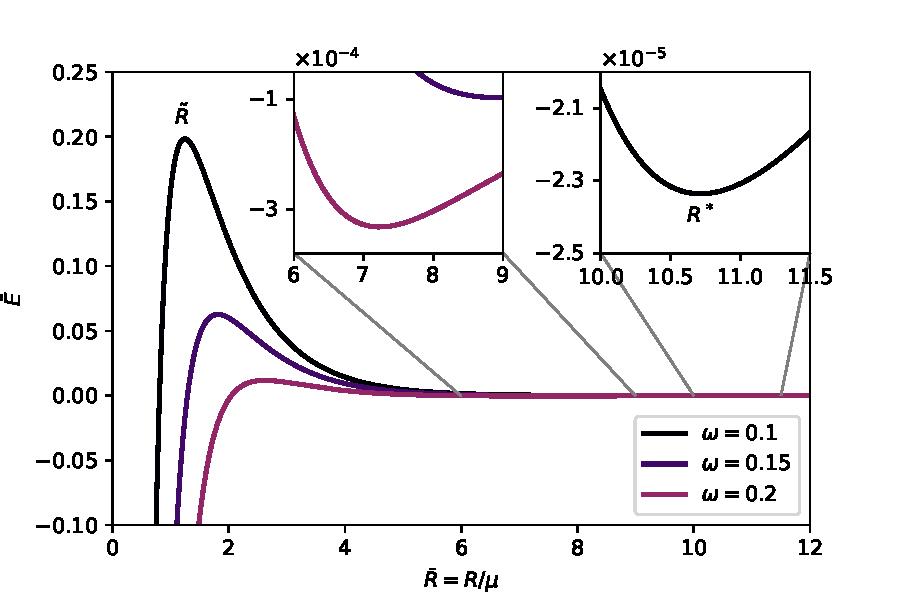
\includegraphics[width=12cm]{figures/3-elastic-figs/Epi2pi2_multiple_w.pdf}
\caption{Two body strong-strong interaction. This is the regime we focus on. The maximum $\bar{E}$ defines the $\tilde{R}$ and the stable equilibrium at $R^*$ is shown in the inset.}
\label{fig:ss}
\end{figure}
\begin{figure}[h]
\centering
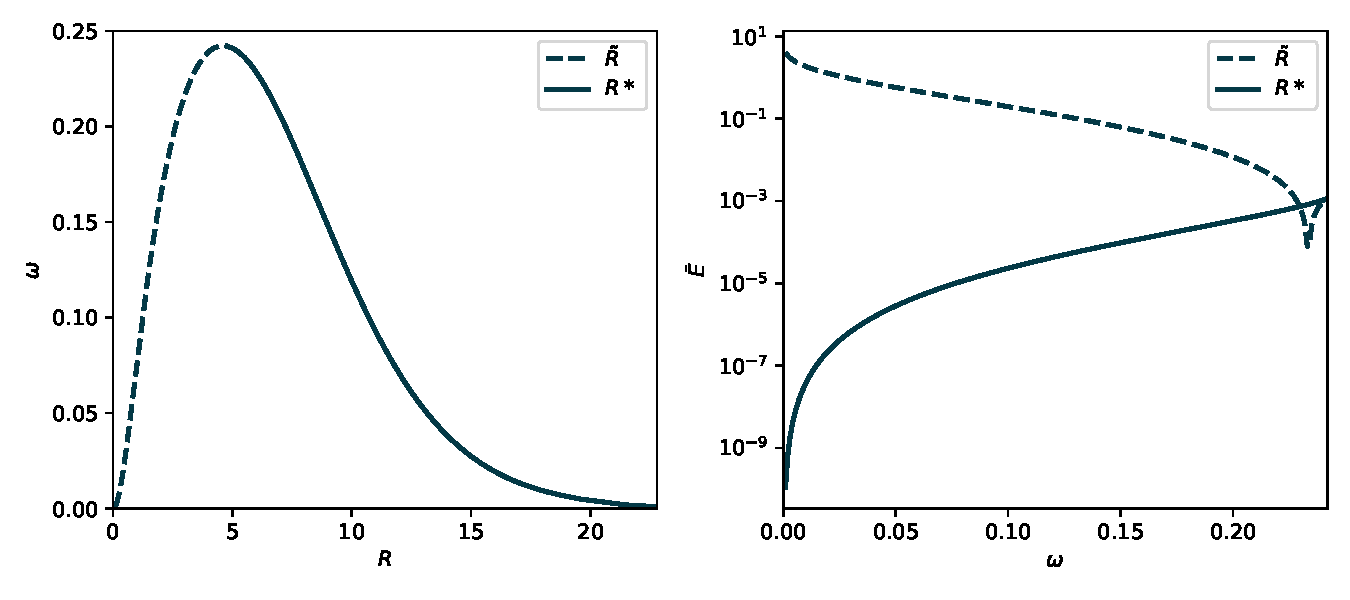
\includegraphics[width=12cm]{figures/3-elastic-figs/bifucation_di_energy.pdf}
\caption{Bifurcation diagram showing how the existence of equilibrium solutions depends the anisotropy parameter, $\omega$. The two colours are the $\tilde{R}$ and $R^*$ equilibria.}
\label{fig:Rbifur}
\end{figure}

\section{Systems of Interacting Inclusions}

Armed with this potential describing the interactions between curvature inducing inclusions, we can explore the structures and dynamics of various configurations of inclusions. The mosaic structure of the lipid bilayer allows for in plane fluid flows with high viscosity. Forces acting on inclusions embedded in a lipid bilayer will therefore cause motion as the flows allow the system to relax and find an energy minimum. Due to the high viscosity, we expect the motion to be overdamped and so each inclusion undergoes a gradient descent in the energy of the system, given by the interaction potential derived earlier. Continuing with the flat membrane approximation, we take the gradient in the $x-y$ reference plane which we used to construct the Monge parameterisation. Following equation \ref{eq:efull} we write the energy of the system as
\begin{equation}
        E= TA_0 + \kappa\xi^2 E'
\end{equation}
where $TA_0$ is constant and $E'$ is the nondimensional energy that we minimised over. The motion of each variable follows
\begin{equation}
    \dot{q_i} = \mu_q \times F_{q_i} =-\mu_q \frac{\partial E}{\partial q_i}.
\end{equation}
where $q$ is either $x$, $y$, or $\phi$. When the energy is at a minimum in all variables, the configuration will not evolve in time and we call this a stationary configuration. The evolution of the non-dimensionalised variable now becomes
\begin{equation}
    \dot{\bar{q_i}} = -\underbrace{\mu_q \frac{\mu^2}{\kappa \xi^2\alpha^2\pi L^2}}_{\bar{\mu}_q}\frac{\partial \bar{E}}{\partial \bar{q_i}}
    \label{eq:overdamp}
\end{equation}
where $\bar{\mu}_q$ has units of inverse time.  From the $x-y$ symmetry of an infinite membrane, we expect $\bar{\mu}_x = \bar{\mu}_y$ and mobilities are connected to diffusivities via the Einstein relation ($D=\mu k_B T$). The ratio of the translational and rotational diffusivity $D_T/D_R\sim a^2$ where $a$ is the radius of the circular inclusion and $a \ll 1$. As such we expect that $\bar{\mu}_x, \bar{\mu}_y \gg \bar{\mu}_{\psi}$ so that the orientation of the inclusions relaxes much faster than position. Here we often take $\bar{\mu}_{\psi} = 10 \bar{\mu}_x = 10\bar{\mu}_y$ and time is non-dimensionalised by $t \rightarrow  t'/\bar{\mu}_x$. \todo{Could we also make a scaling argument here about how these parameters should scale with $L$? This might make more sense that to use Einstein relation which raises questions about modelling the noise. \cite{chou_statistical_2001} rotational timescales usually less than translational.}

\section{Rings, Lines and Lattices}

\subsection{Rings}

There are many possible ways to arrange $n$ inclusions, with each inclusion being described by two positional coordinates an angle describing the orientation. This creates a huge space of possible inclusion configurations, however one particularly simple choice is to consider inclusions spaced evenly on a circle. We can explore the stability of such configurations and ask how this stability changes depending on the asymmetry parameter ($\omega$), or the spacing between the inclusions. We restrict the study of configurations where all inclusions are separated by at least $\Tilde{R}$ to prevent the collapse of structures caused by diverging interaction energy for small separations.

The ring is parameterised by the number of inclusions, $n$, and their distance, $l$, from a central point. This forms a regular polygon of edge length $l_e = 2l\sin(\pi/n)$ - the separation between neighbouring inclusions. We label each inclusion from $1$ to $n$ with the $i^{\text{th}}$ at position $(l\cos(2\pi i/n),l\sin(2\pi i/n))$ however, there are two choices of $\psi_i$ for the inclusions to form a maximally symmetric arrangement. These arrangements are when the the axis of each inclusion either points radially ($\psi_i = 2\pi/i$) or tangentially ($\psi_i = 2\pi/i+\pi/2$) and Fig. \ref{fig:polys2ring} shows these configurations. We can calculate the energy as a function of the radial separation. Numbering the inclusions from $1$ to $n$, the energy for a symmetric arrangement of $n$ inclusions is given by
\begin{equation}
\bar{E}_{n}(l) = \frac{n}{2}\sum_{i=1}^{n-1} \bar{E}_{xy}(l,l\cos(2\pi i/n),0,l\sin(2\pi i/n),0,2\pi i/n)
\label{eq:ring_sum}
\end{equation}
where rather than summing over all pairs we just note the $n$-fold rotational symmetry. The factor $n/2$ prevents double counting and when $n=2$, we recover the two body interaction energy, $\bar{E}_2 = \bar{E}_{xy}\left(x_1,x_2,y_1,y_2,\psi_1,\psi_2\right)$ given by (\ref{eq:exy}).

\begin{figure}[h!]
\centering
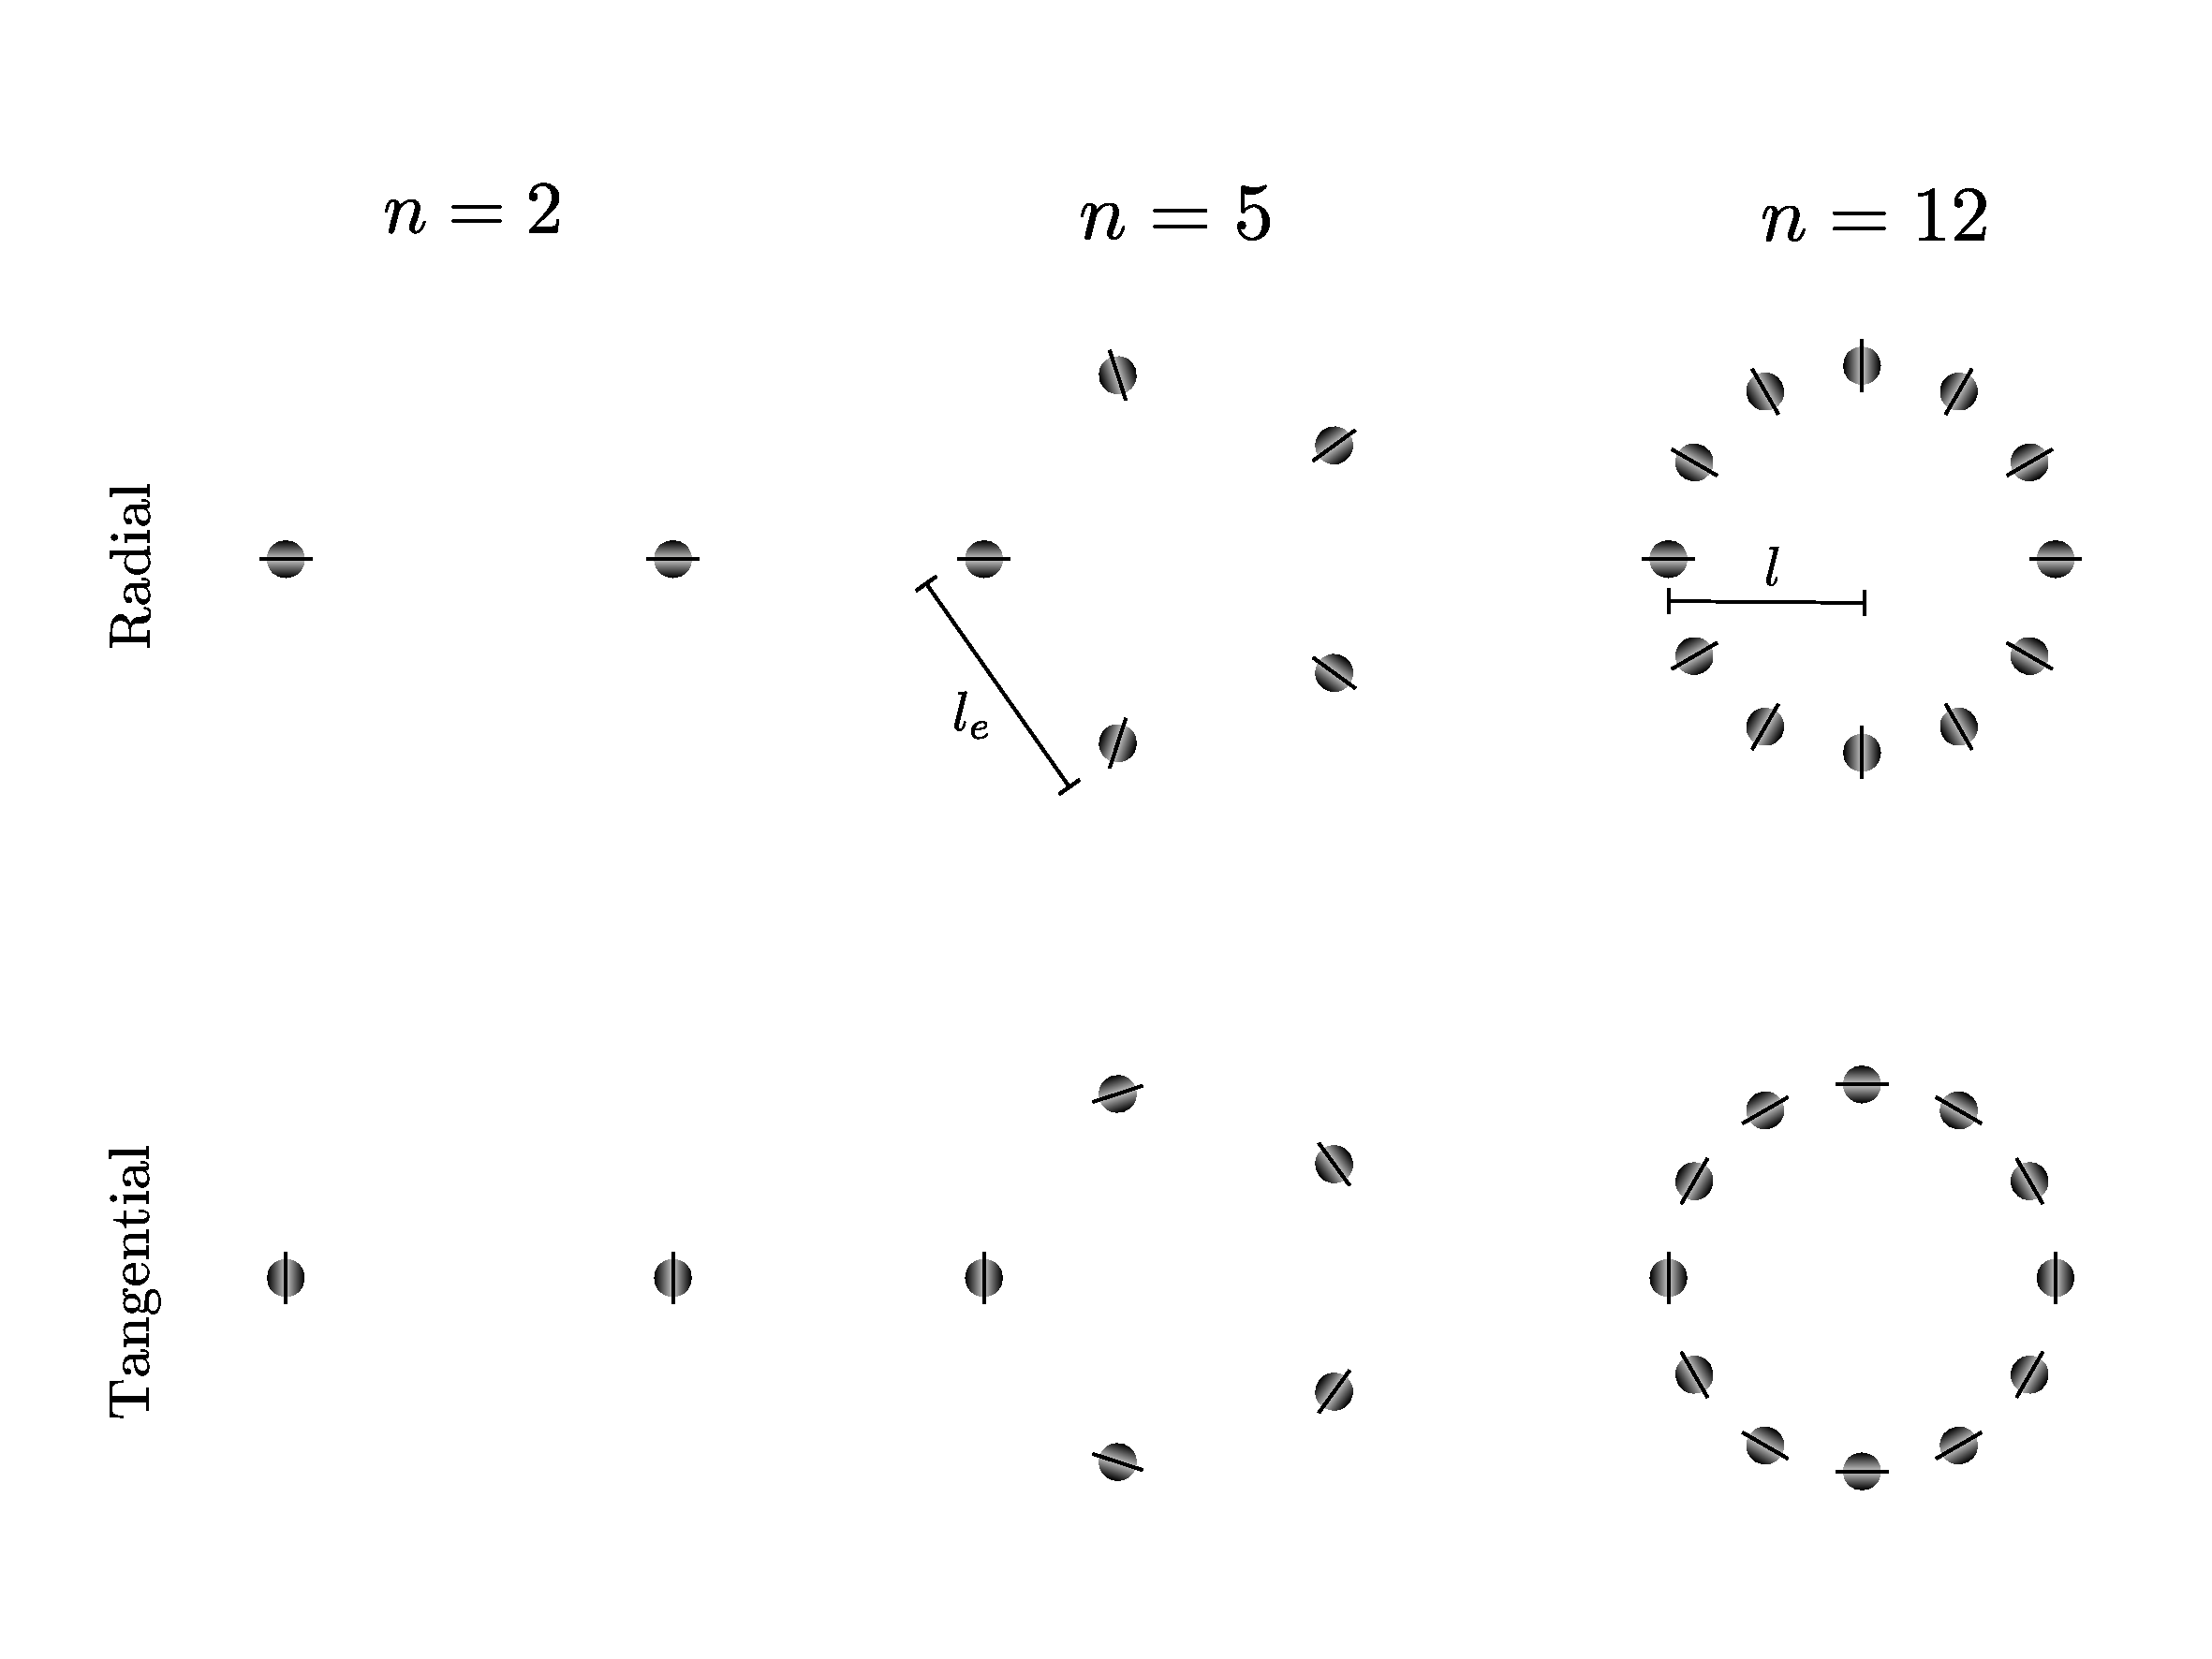
\includegraphics[width=14cm]{figures/3-elastic-figs/n_rings.pdf}
\caption{Radial and tangential setup for rings of $n=2,5,12$.}
\label{fig:polys2ring}
\end{figure}

For a ring of $n$ inclusions, there is some edge length, $l_e(n)$ that minimises the energy of the configuration. This equilibrium ring size can be determined numerically and is shown in Figure \ref{fig:Efnl} for varying $n$ and for two different values of $\omega$. There are two different values of $l_e$ for each $n$: the inclusion separation that minimises the radial configuration, $l_e^R(n)$, and similarly for the tangential configuration $l_e^T(n)$.

\begin{figure}[h]
\centering
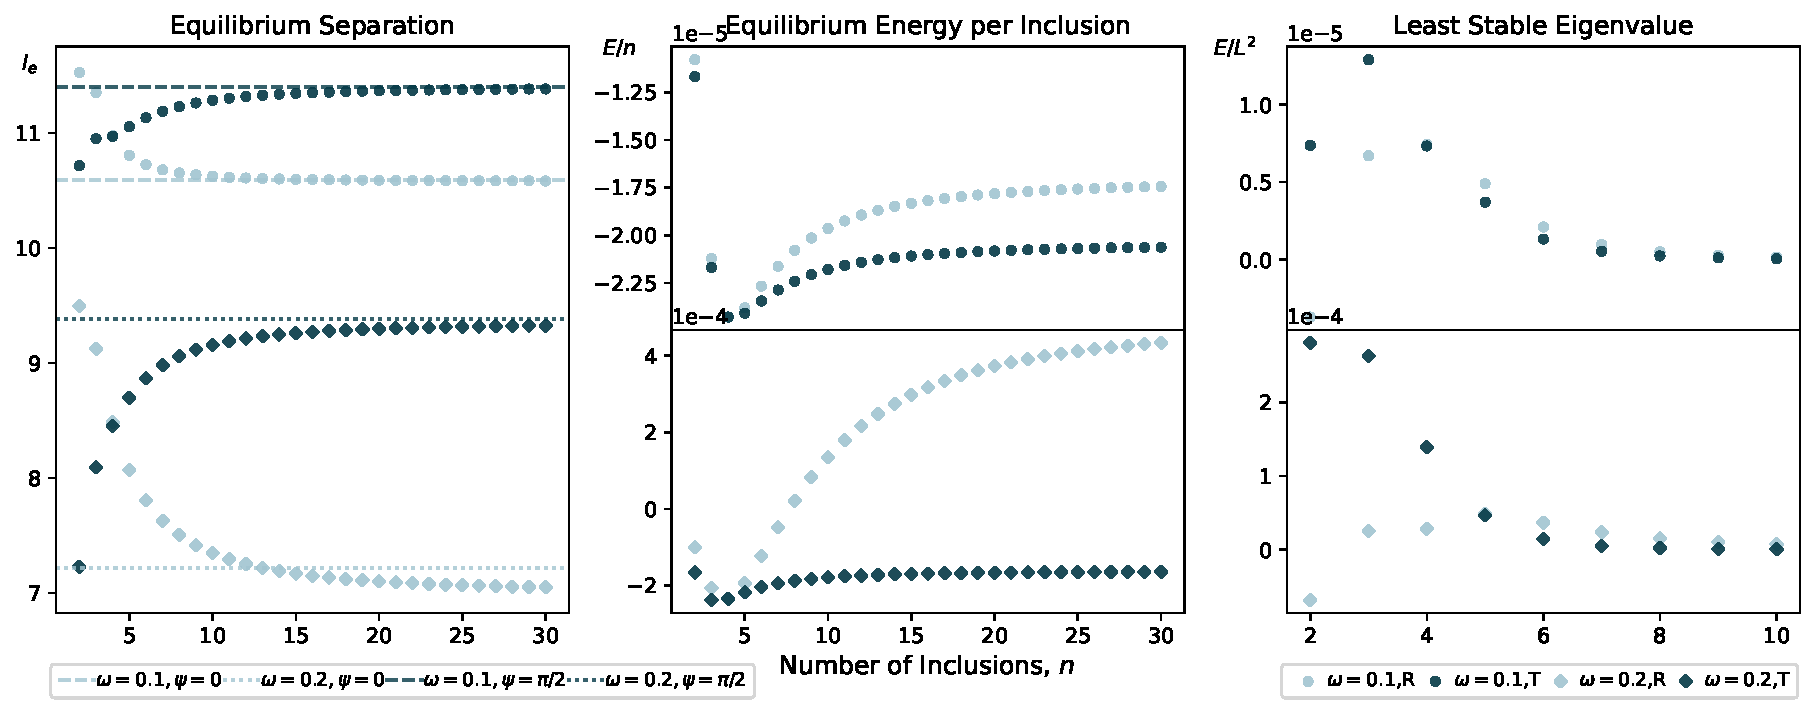
\includegraphics[width=15cm]{figures/3-elastic-figs/polys_multiple_w.pdf}
\caption{Equilibrium inclusion to inclusion separation for inclusions with $\omega=0.1$. Both the radial and tangential configurations are shown. The radial configuration all have $\psi^R_i=2\pi i/n$, compared to the tangential case of $\psi^T_i=2\pi i/n+\pi/2$. \todo{Haven't been able to figure out the $\omega=0.2, \psi=0$ doesn't line up.}}
\label{fig:Efnl}
\end{figure}

As $n$ becomes larger $l_e^T(n)$ is closer to $l_e^R(2)$ than $l_e^T(2)$ (and similarly the other way around). This can be understood as follows: for large $n$, adjacent inclusions in the tangential configuration look very similar to the radial configuration of the two inclusion case i.e. nearest neighbours for $n=12$ in Fig. \ref{fig:polys2ring} look similar to the setup in the $n=2$ case on the left of the figure. The graph also shows that $l_e^T(4) \approx l_e^R(4)$. This makes sense since the symmetry of the two body interaction means that the adjacent inclusions have the same interaction energy in both the radial and tangential configurations and the only difference between the two configurations is come from the pairs of diagonal inclusions. In fact, only the diagonal energy term that is proportional to $(\cos2\psi_1+\cos2\psi_2)$ is different, between the two arrangements.

The stability of a configuration of inclusions can be determined by studying the eigenvalues of the energy Hessian matrix, $\mathbf{H}$ evaluated at the configuration. Here, the Hessian is defined as
\begin{equation}
    \mathbf{H}_{ij}=\frac{\partial^2 \bar{E}}{\partial q_i \partial q_j}.
\end{equation}
If the Hessian is positive semidefinite, $\mathbf{H} \succeq 0$, all of the eigenvalues are positive and the energy increases under any perturbation. This means the equilibrium is stable and under the overdamped dynamics, the system will approach this minimum state from other configurations in the basin attraction. The Hessian and the eigenvalues can be calculated for finite rings and for ring sizes. For any $n$ there are three zero eigenvalues that correspond to the symmetries of the energy: two orthogonal translations of all inclusions and a rotation of the position and angle of all inclusions. In addition to these modes, for $n>2$ all other perturbations increased the energy of the system and rings of inclusions of all sizes are stable.

The Hessian, $\mathbf{H}$, is a $3n\times3n$ matrix and for larger numbers of inclusions, it is hard to extract any meaning from the resulting eigenvectors. Since we expect the translational dynamics to be much slower than the rotational dynamics, we can reduce the number of degrees of freedom by considering only the rotational degree of freedom for each inclusion. Perturbations in the angle are always stable, however it is instructive to study the corresponding eigenmodes. When $n$ is even for both the radial and tangential configurations, the least stable mode - i.e. the mode with the least positive eigenvalue - is a mode with the angles all perturbed by the same magnitude, but with alternating sign between adjacent inclusions, i.e. $\delta\phi_i = (-1)^{i}|\delta\phi|$. For rings with odd numbers of inclusions these alternating rotations would create a mismatch between the first and $n^{\text{th}}$ inclusions and so this might not be the least stable mode. In fact, when $n$ is odd and not very small, the eigenvector with the lowest eigenvalue still corresponded to rotating adjacent inclusions in opposite directions however the magnitude of these rotations varies in such a way that at the mismatch the magnitude of the rotation is very small. When $n=2$, the equivalent radial configuration is unstable, however and the unstable mode is given by an equal and opposite rotation of each inclusion.
% \todo{maybe link to the 2 body interaction}

% \begin{figure}[h]
% \centering
% 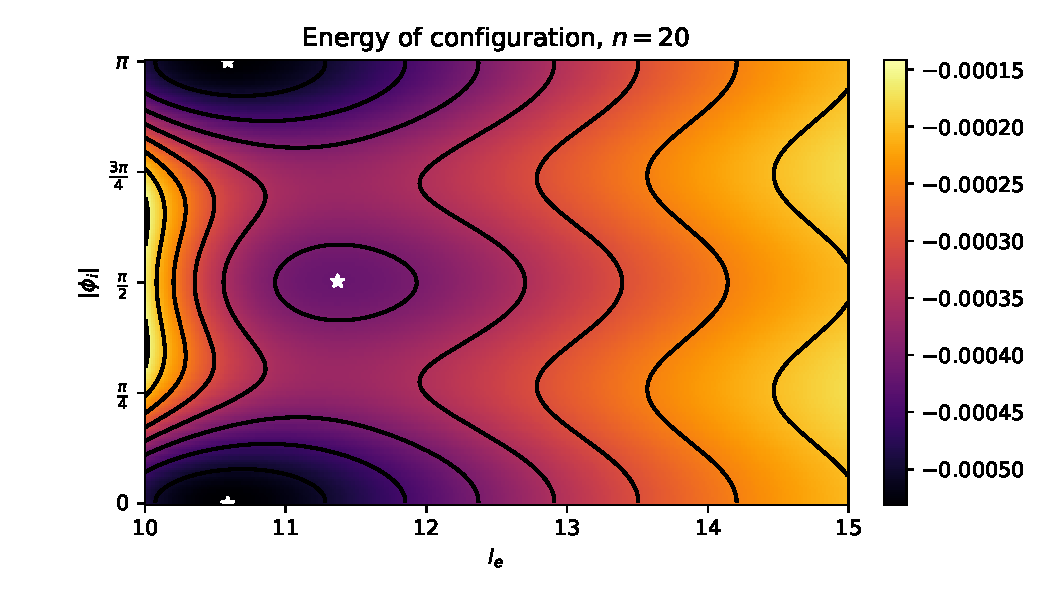
\includegraphics[width=12cm]{figures/3-elastic-figs/ring20sized2.pdf}
% \caption{Interaction energy for a ring of $n=20$ inclusions. The energy is plotted as the inclusion separation and alternating mode perturbation are varied.}
% \label{fig:ring20}
% \end{figure}
\notyet{
\begin{figure}[h!]
\centering
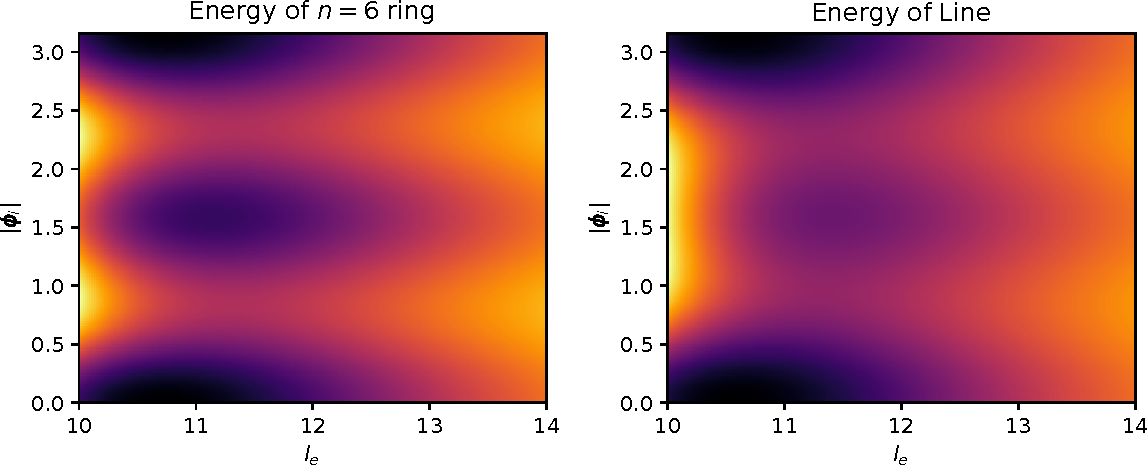
\includegraphics[width=15cm]{figures/3-elastic-figs/energy_line_vs_6_tight.pdf}
\caption{Interaction energy per inclusion for an infinite line inclusions and for a ring of $n=6$ inclusions. The energy is plotted as the inclusion separation and alternating mode perturbation are varied.}
\label{fig:lineenergy}
\end{figure}
}
\begin{figure}[h!]
\centering
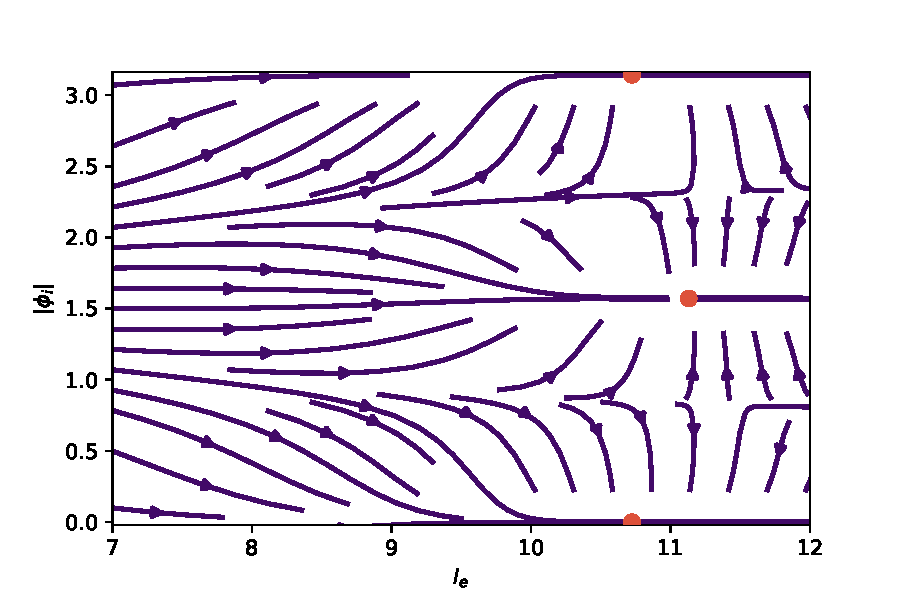
\includegraphics[width=12cm]{figures/3-elastic-figs/streams.pdf}
\caption{Stream plot showing gradient descent for a ring of inclusions in the reduced paramter space of the alternating angular modes at various inclusion-to-inclusion separations. Shown for n=[], $\omega=0.1$ and the key featrures are the same for $\omega=0.2$.}
\label{fig:ring_stream}
\end{figure}

Focusing on a ring with even $n$ number of inclusions, this vector with alternating signs for the rotation connects the radial and tangential configurations. For example starting at the radial configuration, if we perturb all angles by $\delta\phi_i = (-1)^{i}\pi/2$, the system will transition to the tangential configuration. This path represents a trajectory between the two configurations with constant ring radius $l_e$ that initially requires the minimum energy. Varying this parameter, $|\delta\phi|$, and $l_e$ we can explore the energy landscape of these configurations in a massively reduced parameter space that will still give a good representation of the stability of the system. \notyet{\todo{can we get an energy barrier in this space for these?}}

Fig. \ref{fig:ring_stream} shows the gradient descent flow of a ring of inclusions constrained to be evenly radially distributed with an inter inclusion length of $l_e$, and with orientation perturbations that alternate when measured from the radial configuration. The minima for the two maximally symmetric cases are shown by the red dots and as expected the system will approach these two stable configurations anywhere in the phase space. At large $l_e$ the system will approach the nearest configuration in angular space, however at low separations the system approaches the radial ($|\phi_i|=0$) configuration for a wider range of angles. Despite being a subspace of all possible configurations, this observation is informative of the basin of attraction of these two equilibria in all configuration space and indeed when simulating the gradient descent of a random set of pertubations, it is observed that the radial emerges when systems are initialised at smaller $l_e$.

% \subsubsection{Potential from Rings}
% Rings of inclusions will still interact with other inclusions in the pairwise fashion. An additional inclusion outside of a ring of inclusions will cause a minor perturbation of the equilibrium separation of the ring and so we model the ring as being fixed at it's unperturbed separation. If we ignore this minor perturbation, the interaction potential felt by an external inclusion is the sum of contributions from each inclusion in the ring. This interaction is described by three parameters: the  separation between the inclusion and the centre of the ring  $R_\text{ext}$, the angle of the  inclusion $\psi_i$, and the global rotation of the ring $\psi_r$. \todo{Dont even think that the equation below is correct!? - brackets issues I think}
% \begin{equation}
%     E_{\text{ext}} = \sum_N E_2(\sqrt{R_\text{ext}+l_e\sin(2\pi N/5 + \psi_r)^2+l_e\cos(2\pi N/5 + \psi_r)^2}, 2\pi N/5), 
% \end{equation}
% \begin{figure}[h]
% \centering
% \includegraphics[width=12cm]{figures/3-elastic-figs/ring20lower.pdf}
% \caption{Interaction energy for a ring of $n=20$ inclusions at closer separations. The energy is plotted as the inclusion separation and alternating mode perturbation are varied.}
% \label{fig:ring20lower}
% \end{figure}

% \subsection{Random Thoughts}

% Compare e.g. a lattice of size with a ring with all inclusions in there

% Here we investigate the lower density structure formed by anisotropic inclusions and focus on the sturtures that form in the limit of lower densities.

% In this dilute limit, L is large and therefore tension is strong..?

\subsection{Lines}

\subsubsection{Infinite Lines}
As the number of inclusions in the ring increases, the length between neighbouring inclusions, $l_e$, converges to a constant equilibrium value and the ring radius tends to infinity. In the limit this ring of inclusions becomes a line of inclusions separated by $l_e$, and with all inclusions having the same orientation, either $\psi_i=0$ or $\pi/2$ which are analogous to the limits of the tangential or radial rings respectively. Similarly to rings of inclusions, we can explore the energy landscape of the line. Since there are infinitely many inclusions, we expect the energy of the configuration to be infinite. The energy of the interacting inclusions will still be pairwise and as such
\begin{align}
    \bar{E}_{line} &= \sum_{i\neq j}\bar{E}_2(R_{ij}, \pi/2, \pi/2) = \sum_{i=-\infty}^{\infty}\sum_{j=i+1}^{\infty}\bar{E}_2(R_{ij}, \pi/2, \pi/2) \\
    &= \frac{1}{2}\sum_{i=-\infty}^{\infty}\sum_{j=1}^{\infty}\left(\bar{E}_2(l_e \times j, \pi/2, \pi/2) + \bar{E}_2(-l_e \times j, \pi/2, \pi/2)\right) \\
    &= \sum_{i=-\infty}^{\infty}\sum_{j=1}^{\infty}\bar{E}_2(l_e \times j, \pi/2, \pi/2) 
\end{align}
where we can identify the energy \textit{per inclusion} of the line as $\sum_{j=1}^{\infty}\bar{E}_2(l_e \times j, \pi/2, \pi/2)$. \notyet{Approximating the sums as integrals using the Euler-Maclaurin formula gives a very large error. However, we expect that this sum will converge due to the form of the pairwise interaction.}When $x$ is large, $K_\nu(x)\sim e^{-x}/\sqrt{x}$ and therefore $\sum_{n=1}^\infty K_\nu(nx)$ will converge. We also have $\sum_{n=1}^\infty(1/n^4) = \pi^4/90$ and so the energy per inclusion in an infinite line will be finite.\todo{does this make sense? do we need to talk about the density instead?} The sum over all inclusions can be evaluated and is shown in \todo{Fig \ref{}}.
\notyet{The Bessel functions in the two-inclusion interaction energy decay exponentially with distance in the far field and so the sum of $\sum_i K_0(l_e \times i)$ will converge, as will the sums for the other Bessel functions. The remaining term in the energy $\sim\sum_i R^{(l_e \times i)}$ also converges and can be calculated directly.}
% (https://math.stackexchange.com/questions/650966/evaluate-sum-infty-n-1-frac1n4-using-parsevals-theorem-fourier-ser).
% The Euler–Maclaurin formula can convert sums to integrals upto some correction term. This can convert the sum of infinite Bessel function into an integral, however this provides bad accuracy. For example, consider the term in the energy that goes like $K_{0}(R)$. This term's contribution to the energy per inclusion is given by 
% \begin{equation}
%     \sum_{i=1}^{\infty}E_2(i\times l, \phi_i) =
%     \int_m^{n}f(x)dx + \sum _{k=1}^{p}{{\frac {B_{k}}{k!}}\left(f^{(k-1)}(n)-f^{(k-1)}(m)\right)}+R_{p}
% \end{equation}
% \begin{align}
%     \sum_{i=1}^{\infty}E_2(i\times l, \phi_i) &=
%     \int_m^{n}f(x)dx + \sum _{k=1}^{p}{{\frac {B_{k}}{k!}}\left(f^{(k-1)}(n)-f^{(k-1)}(m)\right)}+R_{p} \\
%     &={\frac {f(m)+f(n)}{2}}+{\frac {1}{6}}{\frac {f'(n)-f'(m)}{2!}}-{\frac {1}{30}}{\frac {f'''(n)-f'''(m)}{4!}}+{\frac {1}{42}}{\frac {f^{(5)}(n)-f^{(5)}(m)}{6!}}-\int _{m}^{n}f^{(6)}(x){\frac {P_{6}(x)}{6!}}\,dx\\
% \end{align}
% #####
For rings of inclusions, often we studied the least stable perturbation of the orientations of the inclusions, where each inclusion is rotated by the amount but in opposite directions. A line of inclusions can be perturbed in the same way and again this will transition between a configuration with $\psi_i=0$ to $\psi_i=\pi/2$ for all inclusions, $i$. The energy of a system with $\psi_i=\pm|\delta\phi|$ is given by summing over the inclusions that are rotated in the opposite and same direction separately. The energy of the perturbed line is given by  
\begin{equation}
    E^*_{alt}(\delta\phi) = \sum_{j=1,\text{ odd}}^{\infty}\bar{E}_2(l_e \times j, \pi/2+\delta\phi, \pi/2-\delta\phi) + \sum_{j=2,\text{  even}}^{\infty}\bar{E}_2(l_e \times j, \pi/2+\delta\phi, \pi/2+\delta\phi)
\end{equation}
which simplifies to
\begin{equation}
    \begin{split}
    E^*_{alt}(\delta\phi) =&2\sum_{all}K_0(l_e \times i) - 4\omega\cos(2\delta\phi)\sum_{all}K_2(l_e \times i)+ \omega^2\sum_{even}K_0(l_e \times i)\\
    &+ \omega^2\cos(4\delta\phi)\sum_{odd}K_0(l_e \times i) + \omega^2\cos(4\delta\phi)\sum_{even}\left(K_4(l_e \times i)-\frac{48}{(l_e \times i)^4}\right)
    \end{split}
\end{equation}
and which we can plot, analogously to Fig. \ref{fig:ring20}. The energy profile for the line is shown in Fig. \ref{fig:lineenergy}.
% \begin{figure}[h]
% \centering
% 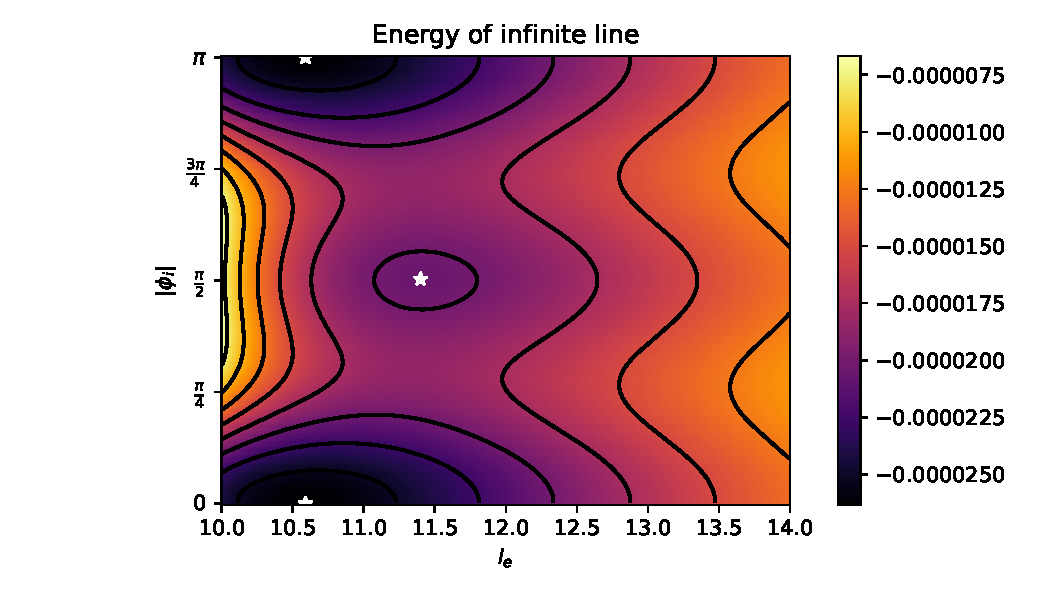
\includegraphics[width=12cm]{figures/3-elastic-figs/line_anti.pdf}
% \caption{Interaction energy per inclusion for an infinite line inclusions. The energy is plotted as the inclusion separation and alternating mode perturbation are varied.}
% \label{fig:lineenergy}
% \end{figure}
Similarly to the rings, the line is stable for both $\psi_i=0$ and $\psi_i=\pi/2$ (for all $i$). The energy minimum is much deeper when $\psi_i=\pi/2$ and this configuration is likely to also have a larger basin of attraction than when $\psi_i=0$. This configuration corresponds to an end-to-end alignment of inclusions with anisotropic geometry\cite{kwiecinski_interactions_2020} and linear aggregates with similar structure have been observed experimentally\cite{simunovic_long-range_2017} and in molecular dynamics simulations \cite{simunovic_linear_2013}. The structure then localises to membrane buds and shows the relevance of elastic interactions even at low densities.

\todo{Is there a way to calculate the energy eigenvalues around stable line?}
\todo{The infinite line stabilises the unstable 2-body interaction.}

\subsubsection{Finite Lines}
Lines with a finite number of inclusions are relevant to study for physically realisable finite systems. The existence of a infinite line would require an infinite system, but also it's likely that shorter lines made up of fewer inclusions will form as intermediates if longer (or even infinite) lines of inclusions were to form. Again, there are two obvious orientations of inclusions to study, but unlike the infinite line each inclusion sees a different arrangement of the other inclusions. As such the equilibrium separation between neighbouring inclusions is not constant but its perturbed slightly depending on their position along the line. The more central inclusions on the lines have a slightly lower separation that those closer to the ends, however this variation was seen to be at most a change of around $2\%$ in the separation across the different inclusions, with the inclusions on the end of the line being more separated.

Again, by studying the Hessian of energy at this stationary configuration, we observe that a finite line of inclusions along the x-axis with the inclusions orientated at $\psi_i=\pi/2$ is stable. This is the configuration similar to the radial ring configuration. However, when the inclusions are orientated at $\psi_i=0$, the finite line is no longer unstable (the tangential ring). For the specific case of a finite line of two inclusions, we saw earlier only one angular orientation was stable. Larger, but still finite lines of inclusions remain unstable and in particular a long oscillatory mode is excited as the line transitions into another configuration. \notyet{\todo{... Talk about the unstable mode}} However, the tangential ring stabilises the two body interaction as exciting the unstable mode would lead to frustration in the system and subsequently raise the energy of the configuration.


\todo{Maybe wait until talking about general configurations/evolution.} Two or more stable finite lines will interact via the elastic mediated interaction. Allowing a group of finite lines to evolve subject to this potential we find that short lines, such as pairs or three co-linear inclusions, will rotate so that their orientations align and then attract to form a large finite line. For larger co-linear groups of inclusions, the initial distribution of the lines can affect the final configuration. As an example, a group of inclusions that approach a line perpendicular to the line of the inclusions will generate different interactions with the different inclusions in the line. As the groups of inclusions approach, this difference in interaction can become large enough to bend the line and transition into a radial ring of inclusions. If the two finite lines of inclusion are aligned initially (but with a spacing to form distinct groups), then the lines will simply coalesce into a longer line. As such, the final configuration depends on the initial distributions of the lines.

\subsection{General Configurations}
Studying rings and lines is useful as these configurations massively reduce the number of coordinates needed to describe the system. However observed inclusion configurations can be initially generated by diffusing proteins binding onto the membranes or as a consequence of driven cellular process that may drag inclusions before detaching. It is therefore useful to explore the elastic forces acting on generic inclusion arrangements which will not necessarily be as symmetric as the rings and lines.

We can explore the evolution of a generic configuration by evolving the system to respond to gradients in energy in the overdamped regime, following the dynamics in (\ref{eq:overdamp}). We choose $\Bar{\mu}_x=\Bar{\mu}_y=\mu_{\phi}/10$, so that the inclusions rotate more quickly in response to gradients of a free energy than they translate and the system is initialised in a random starting configuration with all separations between inclusions greater than $\tilde{R}$. Ensuring this initial separation prevents any of the inclusions from collapsing with diverging energy and allows us to observe the subsequent relaxation of the system to a minimum energy configuration.

As the system is allowed to evolve according to the gradient descent dynamics, the inclusions begin to form aggregates. The system relaxes to a low energy state, where each inclusion is surrounded by a set of neighbouring inclusions that are all approximately $R^*$ away. This makes sense, the interaction from nearby inclusions gives the main contribution to the interaction energy and so the system will try to minimise the two body interaction energy for neighbouring inclusions, however this equilibrium will be slightly perturbed by inclusions that are further away. Similarly to rings, the non-neighbouring inclusions will perturb both the separation and orientation away from being exactly at the two-body equilibrium, and in particular, the anisotropy of the inclusions can generate frustration alter the orientation that minimises the energy.

To visualise the structure of the aggregates, we construct a graph and associated 2D embedding for each configuration. Each inclusion is represented by a node in the graph, embedded at the inclusion location, and edges of the graph connect nearest neighbour inclusions, which we define to be inclusions closer than a distance of $1.3R^{*}$ apart. \notyet{\todo{verify the pre-factor and be consistent}} This threshold is chosen to capture the range of nearest neighbour interactions that were seen from the stable ring and line configurations, without capturing inclusions further away. In particularly, it is good for the threshold to be less than $\sqrt{2}R^{*}$ else diagonal inclusions in a square configuration may appear as nearest neighbours. Constructing this graph and visualising the edges, many of the aggregates formed were comprised of rings of aggregates that formed a lattice of polygons. Additionally, there were also stable configurations containing lines of inclusions that protruded out from the aggregate. \todo{Samples are shown in Fig.}

\todo{some general comments about there being lots of different minimia that the system can end up in, etc., etc.}

\begin{figure}[h]
\centering
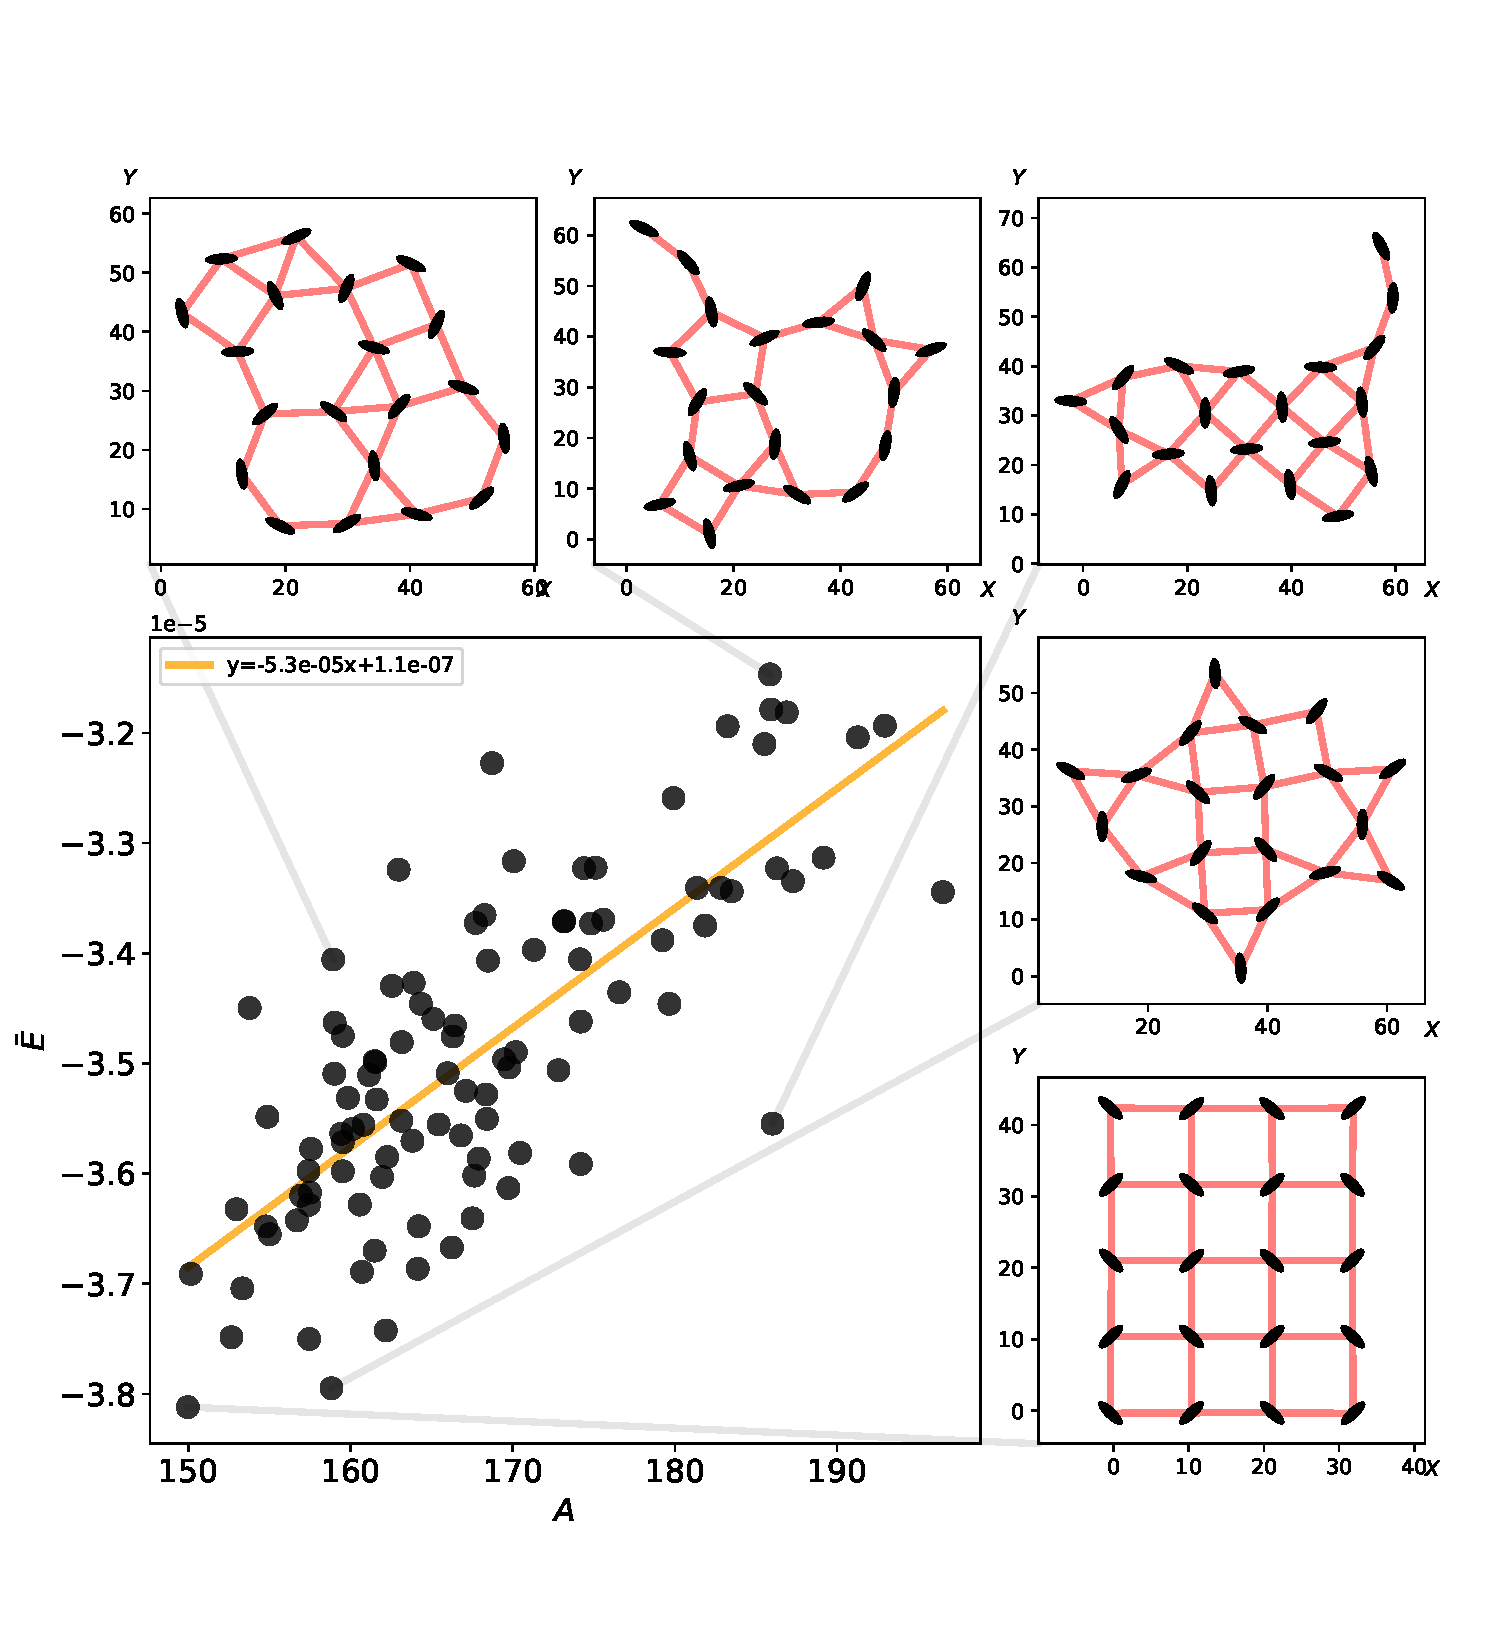
\includegraphics[width=12cm]{figures/3-elastic-figs/autoLatticeEgs100slope.pdf}
\caption{Sample Lattice Figs}
\end{figure}

\subsubsection{Aggregate Structure Depends on Initial Distribution}

The final stable configuration of inclusions depends on the initial configuration. For example, for the case of interacting finite lines the resulting inclusion configuration can be a larger line or a ring, depending on how the initial lines are orientated. This idea holds more generally, and we see a strong dependence of the final stable configuration of inclusions on the initial inclusion configuration. A starting configuration that is closely packed together (still with the minimum separation between inclusions greater than $\tilde{R}$) will initially feel a strong repulsion from nearby inclusions and the inclusions will spread out. During this process, the repulsion dominates, and transient triangular lattices with a lattice spacing less than $R^*$ emerge. As the inclusions are forced to separate by this potential, the average inter inclusion separation approaches $R^*$ and the inclusions rotate to minimise the interaction energy, forming a lattice with many rings of size four, the square configuration seen earlier. In fact, from specific starting configurations a square lattice can form, consisting exclusively of connected groups of four inclusions with alternating, chequerboard pattern of tangential and radial configurations.

In systems of many interacting inclusions, we expect that the square lattice will minimise the configuration energy. Each nearest neighbour will lower the interaction energy, since the two body contribution is negative. The square lattice is the 2D polygonal structure that maximises the number of compatible nearest neighbours and therefore minimises the energy. Not all combinations of regular polygons tile the plane and if they do, there is an additional geometric constraint on the orientation with adjacent polygons. For example, in a triangular lattice, there are six nearest neighbours, however any arrangement of inclusions will be unstable in some mode. This also means that the most dense lattice that can form is the square lattice and so when starting from a high density configuration, the system will encounter this minimum first during its relaxation to an equilibrium.

Fig. \ref{fig:latemerg} demonstrates the formation of the lattice from a random initial inclusions configuration.

\begin{figure}[h]
\centering
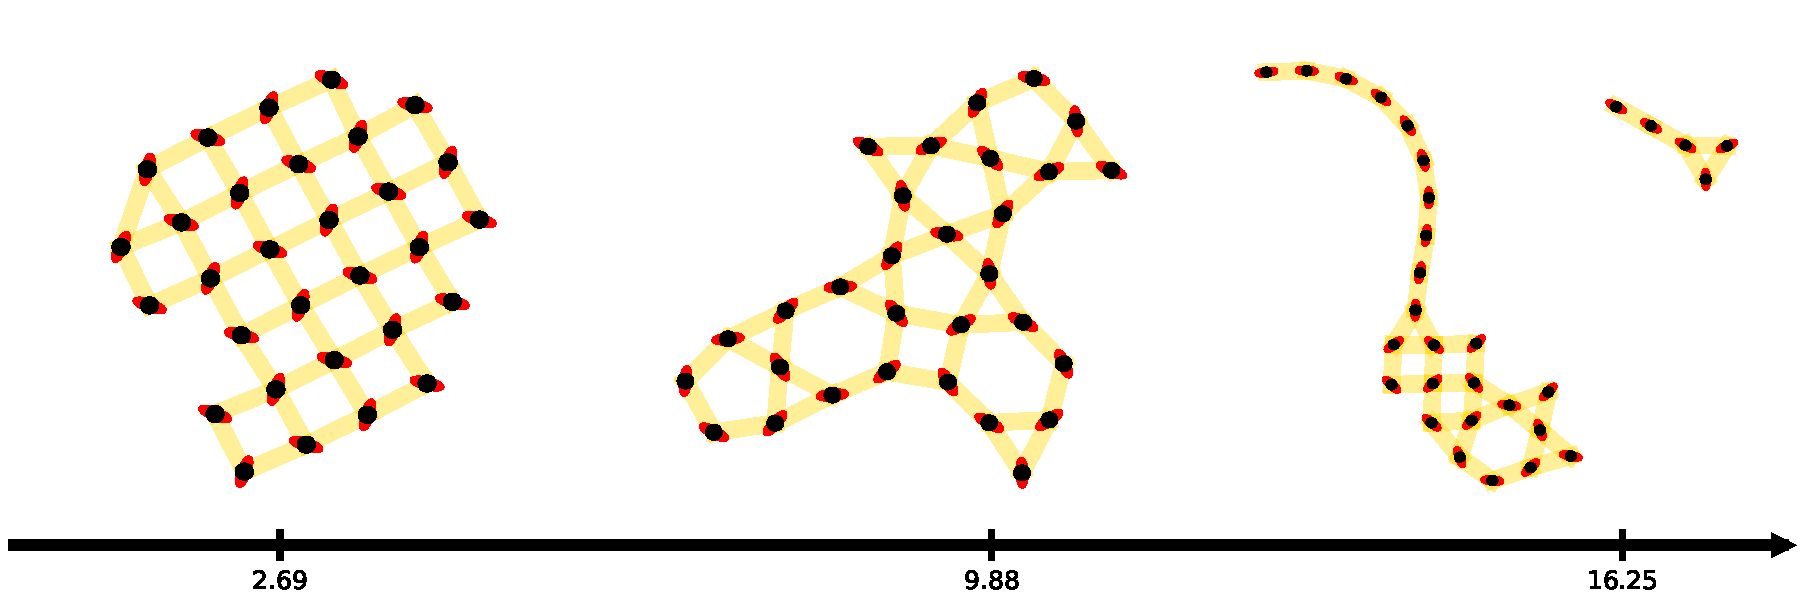
\includegraphics[width=15cm]{figures/3-elastic-figs/different_starts_sample.pdf}
\caption{Examples of the different lattice structures formed from different initial mean nearest neighbours configurations. }
\end{figure}

When inclusions are initialised further apart, all inclusions are initially attracted towards each other. The inclusions are attracted to closer inclusions more strongly and as such two inclusions will suddenly coalesce into the 2-body equilibrium configuration before coalescing with further single inclusions or group of previously coalesced inclusions. This process repeats to form aggregated structures, where groups of coalesced inclusions sequentially grow. In the very low density limit, the spacing between inclusions is very large, so that as they approach the inclusions align and are appended onto the end of existing lines. Multiple inclusions coalescing at similar times, or large lines of inclusions \todo{or just the correct angle really} can perturb the finite lines and generate rings of inclusions. Lines of inclusions will have grown before this happens and thus the rings formed are can be much larger than the polygons of size less than five typically seen for high density initial conditions.

Observed rings of inclusions formed from random configurations result in the radial equilibrium. Again, when the inclusions are initialised at large separation, they will sequentially form a chain in the equivalent of a radial configuration. If the inclusions are perturbed by other inclusions in the system, then this line will collapse into radial ring. Alternatively if multiple inclusions are intialised close together then the streamplot in Figure \todo{ref the stream plot} show that the basin of attraction for the radial configuration is larger than the tangential configuration and as such any rings formed will for a radial ring.

\subsection{Barriers between Configurations}
\todo{incoming}
\notyet{
An interesting question is to do with the transition between the different inclusions configurations. Again, due to the many complex local minima in the space of inclusion configurations, there isn't an obvious way to exhaustively explore the energy landscape and minimum energy barriers associated with transitions between the configurations. Instead, considering simple heurestics and Monte Carlo simulations we can build an intuition for this landscape and how the barriers might affect elastic interactions.

We refer to the barrier of a transition as the minimum increase in the energy required to get from one configuration to another. The transition barrier is the minimum of the maximum energy along the path between two configurations. For any two configurations there exists a path with a maximum energy of intermediate configurations that has 0 energy, which is achieved by sequentially taking the outer most inclusion to infinity and then bringing the inclusions back in one-by-one to build the target configuration. However, often the barrier will be lower than this upper limit.

A particularly simple transition between two energy configurations is the transition where an inclusion is \textit{popped} out of a structure so that a row of three inclusions becomes a triangle. For example, a ring of size $n$ transitioning to a ring of size $n-1$ with a triangular configuration attached as shown in Figure \ref{fig:popout}. 

In order to find the true barrier height, 
To find the barrier height, we would like to find a path between two configurations and minimise the maximum energy along that path. As mentioend exploreing the entire configuration space is not feasible and so instead we use the gradient descent dynamics to aid this search. For example, one might pertub an initial configuration along the direction of a low energy increase and then allow the system to evolve. If the initial perturbation was large enough then the system may approach another energy minimum. However, this approach is limited since the target configuration cannot be controlled and so an alternative approach is to smoothly vary the positional coordinates to approach the target configuration and determine the inclusion orientations by finding the minimum energy subject to inclusion rotations. Again this means that the target orientations cannot be entirely determined, but this provides a feasible method to bound the barrier height between separate configurations.

Also tried other schemes, but they dont really work , lots of time due to the symmetry in everything.   

\todo{Actually we could just start with a configuration, perturb it and allow the system to gradient descent etc.}
    
\begin{figure}[h]
\centering
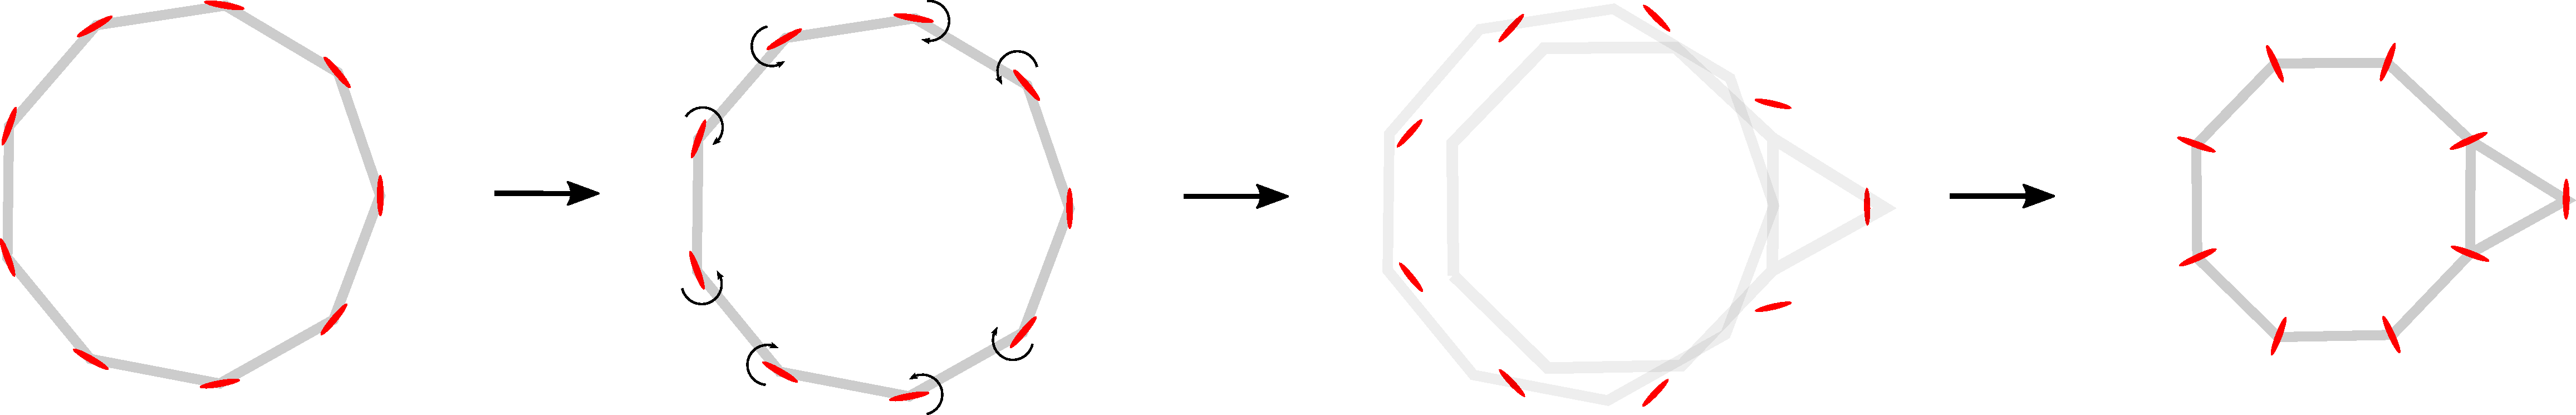
\includegraphics[width=12cm]{figures/3-elastic-figs/barriersScheme.pdf}
\caption{"Pop out" transition between two configurations.}
\label{fig:popout}
\end{figure}

\todo{What about the transition to the 5+3 configuration (i.e the pentagon+triangle), is the method + the barrier similar?}
\todo{Double check Jon's rope pulling?/at some point 'release' it akin to the peel}
\todo{what about the transition for fewer than 6 inclusions/more the 6 inclusions. Try a saimilar method and see what happend}
\todo{Verfiy with simple Monte Carlo stuff.}

\todo{Pull only in xy space and allow both xy angles and actually angles to vary.}

\todo{How does separation scale with tension? could that be a control parameter?}
}
\section{Multi-scale Model for Configurations}
So far, we have only considered the dynamics of inclusions that are initialised sufficiently far apart, such that the equilibrium configurations explore the stable equilibrium around \todo{R (get the right R)}. Inclusions that are separated by a distance less that \todo{this R} will be attracted together by the diverging interaction potential. As the inclusions come close together the separation $R/\epsilon\sim\mathcal{O}(1)$ and so we expect additional terms to appear in the expansion of the interaction potential\todo{if we still use the weak weak form, it just rescales the tension and thus the ratio e/R is still very small - needed for the weak-weak case. Should probably reword this.}. Physically, the inclusions cannot overlap and so we introduce a repulsive term that dominates at small $R$. Inspired by the form of the weak-weak interaction potential we add a term  that goes like $\epsilon^2\frac{4}{R^4}((\alpha_{1}^{(0)})^2+(\alpha_{2}^{(0)})^2)$ and using $\bar{E}=E\mu^2/\pi\alpha^2$ gives
\begin{equation}
\begin{split}
    \bar{E}_2(\bar{R}, \psi_1, \psi_2) &= 2K_0(\bar{R}) + 2\omega K_2(\bar{R})(\cos2\psi_1+\cos2\psi_2) \\
    &+\omega^2\cos(2(\psi_1-\psi_2))K_0(\bar{R})+\omega^2\cos(2(\psi_1+\psi_2))\left(K_4(\bar{R})-\frac{48}{\bar{R}^4}\right) + \epsilon^2\frac{8}{\bar{R}^4}
\end{split}
\end{equation}
This potential now diverges to positive infinity as $R \rightarrow 0$, and for small $\epsilon$, there exists a local minimum, $R_c$, at small separations. The minimum energy still corresponds to $\psi_1 = \psi_2 = \pi/2$ and the separation distance $R_c$ is a functions of $\epsilon$, $R_c=R_c(\epsilon)$. About this equibrlium, the potential is much is much steeper nearby, it is a stiffer equilibrium. Due to the gradients in energy around this minimum, the system's relaxation to equilibrium is therefore dominated by the energy landscape at small separations and intially we will see the dynamics of two inclusions that are in the collapsing regime rapidly converge to the close equilibrium separation, which we will call a \textit{close pair}. Each inclusion in the close pair of inclusions will feel the same forces from external inclusions to leading order in $R_c$ and so we expect the close pair to move together in response to external inclusion arrangments.

\subsection{Effective Super Pairs}
\todo{need to sort out all the $\phi$s vs $\psi$s, need to be consistent.}
The two inclusions close together will exert a strong force on each other and will have some new equilbrium orientation/separation. The new minimum is a much deeper well in the interaction energy, where the two inlcusions are aligned perpendicular to the line between them, but at a much closer separation $R^*_{C}$. Since this well is much deeper and \todo{narrower} than the further out equilibrium, the two inclusions in the close pair will feel strong restoring forces keeping them at this separation. 

We can describe the close pairs by the $x$, $y$ and $\phi$ coordinates describing each inclusion, however similar to interacting particles in an external field, we can also describe the inclusions in a centre of mass coordinate system. In this analogy, the external field is provided by the other far away inclusions which will exert a much smaller force on each inclusion in the pair compared to the force they experience from each other. A natural choice to parameterise the positional coordinates is therefore
\begin{equation}
\begin{split}
x_c = \frac{x_1+x_2}{2}, \quad\text{ and }&\quad y_c = \frac{y_1+y_2}{2} \\
r =  \sqrt{(x_1-x_2)^2+(y_1-y_2)^2}, \quad\text{ and }&\quad \theta = \tan ^{-1}(y_1-y_2,x_1-x_2).
\end{split}
\end{equation}
where describing the orientation of the super pairs is useful as this will be coupled to the individual inclusion alignment. A convenient treatment of the orientations will be to consider the average and difference between the orientations of the two separate inclusions. Simply taking the mean value of $\phi_1$ and $\phi_2$ does not calculate the average orientation in general. Consider two inclusions with $\phi_1=\pi/2-0.01$ and $\phi_2=-\pi/2+0.01$, where the angles describe two similarly orientated inclusions, $\updownarrow$ and $\updownarrow$. The arithmetic mean of this is gives $\phi_C=0$, which gives a very different orientation to both individual inclusions, $\leftrightarrow$ (this cannot be fixed by simply measuring the angles on the domain $0$ to $\pi$, as this simply rotates the problem case, $\phi_1=\pi-0.01$ and $\phi_2=0.01$). The solution is to measure the both angles within the same quadrant, as then the maximum angular difference between the two orientations will be $\pi/2$. Using the properties of the two argument $\arctan$, this can be written in general as
\begin{equation}
\begin{split}
\phi_c &= \frac{1}{2}\arctan\left(\cos2\phi_1+\cos2\phi_2,\sin2\phi_1+\sin2\phi_2\right) \quad\text{ and } \\
\phi_d &= \phi_1 - \phi_2
\end{split}
\end{equation}
where we allow $\phi_d$ to depend on how the separate angles were measured. \todo{discuss that the arctan thing is not actually going to be an issue...}

The new set of coordinates highlights the slow and enslaved variables. From the steep potential around the close equilibrium separation we expect that to leading order $r=R^*_c$ and $\phi_d=0$. We also expect that $\theta= \pi/2 + \phi_c$ and as such the pair of inclusions can be described by three slow variables. However it is not clear whether the gradients in $\phi_c$ or $\theta$ dominate the dynamics - whether the rotation of the pair is limited by the translational motion of the inclusions, or the rotation. Thus, simply setting $\theta= \pi/2 + \phi_c$ or $\phi_c = \theta - \pi/2$ may not capture the behaviour of the inclusion pair. To include both the translation and rotation of the individual inclusions when considering the motion of the pair, we take a linear combination of the two to eliminate the slow variable and define
\begin{equation}
    \psi_c = \frac{\theta + \kappa (\frac{\pi}{2} + \phi_c)}{1+\kappa} \quad\text{ and }\quad \psi_d = \theta - \left(\frac{\pi}{2} + \phi_c \right)
\end{equation}
where $\kappa$ is to be determined, $\psi_c$ gives the overall orientation of the pair and $\psi_d$ is enslaved by the fast variables to be zero.

The overdamped dynamics can be written as
\begin{equation}
    \frac{\dd \mathbf{X}_i}{\dd t}= \sum_{j}M_{ij}\frac{\dd E}{\dd \mathbf{X}_j},
\end{equation}
where we define the coordinate vector $\mathbf{X}=(x_1, x_2, y_1, y_2, \phi_1, \phi_2)$ and the mobility matrix, $\mathbf{M}=\mathrm{diag}(\mu_t, \mu_t, \mu_t, \mu_t,\mu_r, \mu_r)$. As a matrix equation this is
\begin{equation}
    \frac{\dd \mathbf{X}}{\dd t}= \mathbf{M}\frac{\dd E}{\dd \mathbf{X}}.
\end{equation}
Defining the new coordinate vector, $\mathbf{Y}=(x_c, y_d, \psi_c, r, \psi_d, \phi_d)$ and the Jacobian between these two coordinate systems, $\mathbf{J}$, the new variables will evolve in a similar fashion
\begin{equation}
    \frac{\dd \mathbf{Y}}{\dd t} = \mathbf{J}\frac{\dd \mathbf{X}}{\dd t} = \mathbf{J}\mathbf{M}\frac{\dd E}{\dd \mathbf{X}} = \underbrace{\mathbf{J}\mathbf{M}\mathbf{J}^{-1}}_{\mathbf{M'}}\frac{\dd E}{\dd \mathbf{Y}}.
\end{equation}
This gives the same evolution equation, but with a modified mobility matrix. Evaluating this new mobility matrix gives
\begin{equation}
    \mathbf{M}'=
\left(
\begin{array}{cccccc}
 \frac{\mu_t}{2} & 0 & 0 & 0 & 0 & 0 \\
 0 & \frac{\mu_t}{2} & 0 & 0 & 0 & 0 \\
 0 & 0 & \frac{\kappa ^2 \mu_r+\frac{4 \mu_t}{(x_{1}-x_{2})^2+(y_{1}-y_{2})^2}}{2 (\kappa +1)^2} & 0 & \frac{\frac{4 \mu_t}{(x_{1}-x_{2})^2+(y_{1}-y_{2})^2}-\kappa  \mu_r}{2 (\kappa +1)} & 0 \\
 0 & 0 & 0 & 2 \mu_t & 0 & 0 \\
 0 & 0 & \frac{\frac{4 \mu_t}{(x_{1}-x_{2})^2+(y_{1}-y_{2})^2}-\kappa  \mu_r}{2 (\kappa +1)} & 0 & \frac{\mu_r}{2}+\frac{2 \mu_t}{(x_{1}-x_{2})^2+(y_{1}-y_{2})^2} & 0 \\
 0 & 0 & 0 & 0 & 0 & 2 \mu_r \\
\end{array}
\right).
\end{equation}
Coupling $\theta$ and $\phi_c$ introduces off diagonal terms in the mobility matrix, that depend on the other coordinates in the system. However choosing $\kappa = 4\mu_t/(r^2\mu_r)$ these off-diagonal terms vanish and at the pair equilibrium we expect, $r=R_C^*$ which is constant and therefore we take $\kappa = 4\mu_t/((R_C^*)^2\mu_r)$.\todo{$\mu_r$ is larger, but $r$ is small, is this going to cause issues about the separation of the time scales?} \todo{Say about: $\kappa$ implies the relative contribution of each process in limiting the rotation of the pair} The mobility matrix is fully diagonal,
\begin{equation}
    \mathbf{M}'=\mathrm{diag}\left(\frac{\mu_t}{2},\frac{\mu_t}{2},\frac{2 \mu_r \mu_t}{r^2\mu_r+4\mu_t},2\mu_t,\frac{\mu_r}{2}+\frac{2 \mu_t}{r^2},2\mu_r\right)
\end{equation}
and we therefore have a reduced system where we set $r=R^*_C$, $\psi_d=0$, and $\phi_d=0$. We can evolve the remaining three variables, the \textit{reduced system}, describing the pair of inclusions using the overdamped dynamics, but with transformed mobilities.

In addition to the modified mobility, we need to calculate gradients of the energy in the reduced system. Using the general two body interaction energy $E_2(R, \psi_a, \psi_b)$ from \todo{equation} we label a configuration of $n$ inclusions with the inclusions $1$ and $2$ being in a close pair. The energy of the configuration with the pair is therefore
\begin{equation}
\begin{split}
    E_{overall} &= \left(\sum_{i=3}^{n}\sum_{i=j+1}^{n}E_{2}\big(R_{ij}, \psi_i-\theta_{ij}, \psi_j-\theta_{ij}\big)\right) + E_{2}\big(R_{12}, \psi_1-\theta_{12}, \psi_2-\theta_{12}\big)\\
    &+ \sum_{i=3}^{n}\Big(E_{2}\big(R_{i1}, \psi_i-\theta_{i1}, \psi_1-\theta_{i1}\big) + E_{2}\big(R_{i2}, \psi_i-\theta_{i2}, \psi_2-\theta_{i2}\big)\Big)
\end{split}
\end{equation}
where we split the interaction energy into contributions from inclusions not in the pair, inclusions in the pair, and an inclusion in the pair and interacting with an inclusions away from the pair. The first term is unaffected by the coordinate transformation. The second term is the interaction between the two inclusions in the pair and this term drives the fast dynamics in the system, constraining the pair of inclusions to be at their equilibrium separation and orientation. This contribution can be written as $E_{2}\big(R_{12}, \psi_1-\theta_{12}, \psi_2-\theta_{12}\big) = E_{2}\big(r, \pi/2, \pi/2\big)$ which will be constant for the slow dynamics. Since the inclusion in the pair are close together, that is $r \ll 1$, they are also close to $x_c$ and $y_c$ and so we can expand the energy around these points. For inclusion $1$ this is
\begin{equation}
\begin{split}
    E_{2}\big(R_{i1}, &\psi_i-\theta_{i1}, \psi_1-\theta_{i1}\big) = \\
    &E_{2}\big(R_{ic}, \psi_i-\theta_{ic}, \psi_c-\theta_{ic}\big) + \left[\left(\frac{\partial E_{2}}{\partial R}\frac{\partial R_{i1}}{\partial x_1}-\left(\frac{\partial E_{2}}{\partial \psi_a} + \frac{\partial E_{2}}{\partial \psi_b}\right)\frac{\partial \theta_{i1}}{\partial x_1}\right)\frac{r}{2}\cos\psi_{c}\right. \\
     &+ \left.\left(\frac{\partial E_{2}}{\partial R}\frac{\partial R_{i1}}{\partial y_1}-\left(\frac{\partial E_{2}}{\partial \psi_a} + \frac{\partial E_{2}}{\partial \psi_b}\right)\frac{\partial \theta_{i1}}{\partial y_1}\right)\frac{r}{2}\sin\psi_{c}\right]_{R=R_{ic}, \psi_a=\psi_i-\theta_{ic}, \psi_b=\psi_c-\theta_{ic}} + \mathcal{O}(r^2)
\end{split}
\end{equation}
where we have $R_{ij} = \sqrt{(x_i-x_j)^2+(y_i-y_j)^2}$ and $\theta_{ij}=\arctan(x_i-x_j, y_i-y_j)$. We can do the same thing for inclusion $2$ which gives an identical expansion except with $r\rightarrow-r$ and so the linear terms in the expansion exactly cancel out in the expansion \todo{Can we write this r/R ? I dont think that is what is it actually...}. As such we can now write the energy as
\begin{equation}
\begin{split}
    E_{overall} &= \left(\sum_{i=3}^{n}\sum_{i=j+1}^{n}E_{2}\big(R_{ij}, \psi_i-\theta_{ij}, \psi_j-\theta_{ij}\big)\right) + \sum_{i=3}^{n}2E_{2}\big(R_{ic}, \psi_i-\theta_{ic}, \psi_c-\theta_{ic}\big) + \mathcal{O}(r^2)
\end{split}
\end{equation}
where the energy has been shifted by the self interaction energy of the inclusion pair. In fact this procedure can be generalised so that the interaction of multiple pairs of inclusions can also be described, where two interacting pairs of inclusions contribute $4 E_{2}\big(R_{ic}, \psi_i-\theta_{ic}, \psi_c-\theta_{ic}\big)$ to the total interaction energy. Recall that we scaled the interaction energy by the magnitude of the monopole mode. An inclusion with the same asymmetry, but different couple the induced curvature would contribution twice as much to the interaction energy which is exactly the effect of the inclusion pair, upto $\mathcal{O}(r^2)$. We can therefore model a pair of inclusions as one single inclusion, with the same anisotropy but twice the monopole mode and a modified translational and rotational mobility \todo{check that we've used $\theta_c$ or $\psi_c$ or whatever at the right time}.

\todo{we expect that increaseing e.g. the mean curvature would icncrease the footprint anad affect the mobility?}

The reduced system can be used to evolve a random configuration of inclusions, that also includes pairs of inclusions that are close together. The pair-to-inclusion and pair-to-pair interactions have the same features as the inclusion-to-inclusion interaction and so we expect that resulting stable configurations will also have similar structure. This is in fact what we find. Resulting stable configurations of inclusions and pairs, have the same polygonal structure, with slight perturbations due to the increased strength of the pair interactions. However, depending an the initial configuration a system containing a par of inclusions might converge to a different final configuration when compared to single inclusions that are initialised with the same starting configuration.
m
\todo{We could do a similar analysis for groups of e.g. three inclusions, but we are focusing on the well separated limit which its unlikely that multiple inclusions will be stuck together.}

\notyet{
\subsection{Effective Super Pairs}  

Could be useful for polymerising systems? \cite{saletti_matrix_2017}

The dynamics of two interacting particles in an external potential can be described as
\begin{align}
    m_1\ddot{\mathbf{r}}\mathbf{_1} = \textbf{F} + \nabla_{\mathbf{r}\mathbf{_1}}E_{\text{ext}} \\
    m_2\ddot{\mathbf{r}}\mathbf{_2} = -\textbf{F} + \nabla_{\mathbf{r}\mathbf{_2}}E_{\text{ext}}
\end{align}
where we can assume the interaction giving the force $\textbf{F}$ is conservative to give so we can define an additional term in the external energy that depends on $(\mathbf{r}\mathbf{_1}-\mathbf{r}\mathbf{_2})$ and consequently the gradient in the different variables picks up the change of sign.
\begin{align}
    m_1\ddot{\mathbf{r}}\mathbf{_1} = \nabla_{\mathbf{r}\mathbf{_1}}E \\
    m_2\ddot{\mathbf{r}}\mathbf{_2} = \nabla_{\mathbf{r}\mathbf{_2}}E
\end{align}
 where $\textbf{F}$ is the equal an opposite force extered by one particle on the other and $E$ is the external potential. Making the transformation in a 1d system, to centre of mass and \textit{difference} coordinates, we write
 \begin{equation}
 \underbrace{\left(
\begin{array}{cc}
 x_C \\
 x_d \\
\end{array}
\right)}_{\textbf{y}} = \underbrace{\left(
\begin{array}{cc}
 \frac{m_1}{m_1+m_2} & \frac{m_2}{m_1+m_2} \\
 1 & -1 \\
\end{array} \right)}_{M} \cdot \underbrace{\left(
\begin{array}{cc}
 x_1 \\
 x_2 \\
\end{array} \right)}_{\textbf{x}}.
\end{equation}
so $y_i = \sum_j M_{ij}x_j$ and thus $\partial y_i / \partial x_j = M_{ij}$ Defining $L=\text{diag}(m_1, m_2)$ we can rewrite the dynamics
\begin{equation}
    \ddot{y}=M \ddot{x}=M L^{-1}\nabla_{\mathbf{x}}E.
\end{equation}
Using the transform 
\begin{equation}
    (\nabla_x E)_i = \frac{\partial E}{\partial x_i} = \sum_j \frac{\partial E}{\partial y_j}\frac{\partial y_j}{\partial x_i} = \sum_j \frac{\partial E}{\partial y_j} M_{ji} = (M^T \nabla_y E)_i
\end{equation}
so $\ddot{y}= M L^{-1} M^T\nabla_{\mathbf{y}}E$ and we therefore define a new effective mass matrix $L_y = (M L^{-1} M^T)^{-1}$ which for the $L$ and $M$ defined above we find
\begin{equation}
    L_y = \left(
\begin{array}{cc}
 m_1+m_2 & 0 \\
 0 & \frac{m_1 m_2}{m_1+m_2} \\
\end{array}
\right)
\end{equation}
which is the usual total and reduced mass. For the overdamped evolution, we consider $\dot{x}=\mu_x\nabla_x$ and for a transformed variable $y$, we get $\mu_y = M\mu_xM^T$. Using the uniform expansions, we expect two inclusions that have been brought together will form a stiff inclusion pair separated by a much smaller equilibrium distance, $r_C$. We can define new transformed variables that describe the position of the centre of mass and relative distance of both spatial coordinate in the system, as well as the angular coordinates. (I think that these coordinated fundamentally miss the coupling between the position and angle.) So we have $v_c = (v_1 + v_2)/2$ and $v_d = (v_1 - v_2)$. The transformation matrix for all three coordinates looks like    
\begin{equation}
    M = \left(
\begin{array}{cccccc}
 \frac{1}{2} & \frac{1}{2} & 0 & 0 & 0 & 0 \\
 1 & -1 & 0 & 0 & 0 & 0 \\
 0 & 0 & \frac{1}{2} & \frac{1}{2} & 0 & 0 \\
 0 & 0 & 1 & -1 & 0 & 0 \\
 0 & 0 & 0 & 0 & \frac{1}{2} & \frac{1}{2} \\
 0 & 0 & 0 & 0 & 1 & -1 \\
\end{array}
\right)
\end{equation}
and we have
\begin{equation}
    \mu_x = \left(
\begin{array}{cccccc}
 \mu_t & 0 & 0 & 0 & 0 & 0 \\
 0 & \mu_t & 0 & 0 & 0 & 0 \\
 0 & 0 & \mu_t & 0 & 0 & 0 \\
 0 & 0 & 0 & \mu_t & 0 & 0 \\
 0 & 0 & 0 & 0 & \mu_r & 0 \\
 0 & 0 & 0 & 0 & 0 & \mu_r \\
\end{array} \right)
\quad
\text{and}
\quad
 \mu_y = \left(
\begin{array}{cccccc}
 \frac{\mu_t}{2} & 0 & 0 & 0 & 0 & 0 \\
 0 & 2 \mu_t & 0 & 0 & 0 & 0 \\
 0 & 0 & \frac{\mu_t}{2} & 0 & 0 & 0 \\
 0 & 0 & 0 & 2 \mu_t & 0 & 0 \\
 0 & 0 & 0 & 0 & \frac{\mu_r}{2} & 0 \\
 0 & 0 & 0 & 0 & 0 & 2 \mu_r \\
\end{array}
\right)
\end{equation}

Consider a system of two close inclusions and one far away. We write the energy in a similar form the two body problem, for $E = E_{12}+E_O$, where $E_{12}$ describes the interaction energy between the two close inclusions and $E_O = E_{13}+E_{23}$. Consider for example the evolution of $x_C = (x_1 + x_2)/2$.  We know
\begin{equation}
    \frac{\partial E_{12}}{\partial x_{1}} = -\frac{\partial E_{12}}{\partial x_{2}}
\end{equation}

...

A better set of transforms will be to use the following


\begin{center}
$\begin{array}{ |c|c| }
\hline
\textbf{New Vars} & \textbf{Old Vars} \\
\hline
x_c & \frac{x_1+x_2}{2} \\
y_c & \frac{y_1+y_2}{2} \\
r & \sqrt{(x_1-x_2)^2+(y_1-y_2)^2} \\
\theta & \tan ^{-1}(y_1-y_2,x_1-x_2) \\
\phi_c & \frac{\phi_1+\phi_2}{2} \\
\phi_d & \phi_1-\phi_2 \\
\hline
\end{array}$
\end{center}
however these are not linear and so to the transformation will not be a constant matrix. We make a transform using the Jacobian

$\left(
\begin{array}{cccccc}
 \frac{1}{2} & \frac{1}{2} & 0 & 0 & 0 & 0 \\
 0 & 0 & \frac{1}{2} & \frac{1}{2} & 0 & 0 \\
 \frac{x_1-x_2}{\sqrt{(x_1-x_2)^2+(y_1-y_2)^2}} & -\frac{x_1-x_2}{\sqrt{(x_1-x_2)^2+(y_1-y_2)^2}} & \frac{y_1-y_2}{\sqrt{(x_1-x_2)^2+(y_1-y_2)^2}} & -\frac{y_1-y_2}{\sqrt{(x_1-x_2)^2+(y_1-y_2)^2}} & 0 & 0 \\
 \frac{y_1-y_2}{(x_1-x_2)^2+(y_1-y_2)^2} & -\frac{y_1-y_2}{(x_1-x_2)^2+(y_1-y_2)^2} & \frac{x_2-x_1}{(x_1-x_2)^2+(y_1-y_2)^2} & -\frac{x_2-x_1}{(x_1-x_2)^2+(y_1-y_2)^2} & 0 & 0 \\
 0 & 0 & 0 & 0 & \frac{1}{2} & \frac{1}{2} \\
 0 & 0 & 0 & 0 & 1 & -1 \\
\end{array}
\right)$
which result in the modified mobilities
\begin{equation}
    \left(
\begin{array}{cccccc}
 \frac{\mu_t}{2} & 0 & 0 & 0 & 0 & 0 \\
 0 & \frac{\mu_t}{2} & 0 & 0 & 0 & 0 \\
 0 & 0 & 2 \mu_t & 0 & 0 & 0 \\
 0 & 0 & 0 & \frac{2 \mu_t}{r^2} & 0 & 0 \\
 0 & 0 & 0 & 0 & \frac{\mu_r}{2} & 0 \\
 0 & 0 & 0 & 0 & 0 & 2 \mu_r \\
\end{array}
\right)
\end{equation}
The new set of coordinates highlights the slow and enslaved variables. From the steep potential around the close equilibrium separation we expect that to leading order $r=R^*_c$ and $\phi_C$. We also expect that $\phi_d = \pi - \theta$. Without looking at the energy gradients, it's not obvious whether the gradients in $\phi_d$ or $\theta$ dominate the dynamics. As such we can take a linear combination of the two to define two new variables
\begin{center}
$\begin{array}{ |c|c| }
\hline
\textbf{New New  Vars} & \textbf{New Vars} \\
\hline
\theta_b & (\theta + \kappa (\pi - \phi_c))/(1+\kappa) \\
\phi_0 & \theta - (\pi - \phi_c) \\
\hline
\end{array}$
\end{center}
where we choose $\kappa$ such that the mobilities are kept to be diagonal. This occurs when $\kappa = 4\mu_t/(r^2\mu_r)$, which slightly complicates the mapping since $\kappa$ depends on one of the new variables. Instead, we use the equilibrium value of $r=R^*_C$ to make the transformed mobility diagonal when the $r$ variable equilibrates, which we expect to happen very quickly due to the steep potential. We therefore have a reduced system where we set $r=R^*_C$, $\phi_0$, and $\phi_d=0$. We can evolve the remaining three variables, the \textit{reduced system}, describing the pair of inclusions using the overdamped dynamics, but with transformed mobilities. If the inclusions in the pair were not at the equilibrium separation, there would be a small error in the dynamics, but comparing the solutions to both the full system and the reduced system showed very good agreement.
}

\section{Discussion and Conclusions}

This work has focused on a specific limit of the membrane mediated interaction between curvature inducing inclusions: when the inclusions induce small curvatures and when the inclusions are far apart. This is a previously understudied regime, with many models considering inclusions that are much closer together. In the well separated limit considered here the effects of the membrane elasticity dominate, without near field interactions, such as steric effects, or changes to the bilayer thickness from the protein binding (we expect this variation to decay exponentially) \todo{cite}.

The anisotropy in the system fundamentally changes the interaction by the introduction of an equilibrium separation, rather than infinite repulsion for the symmetric case. Furthermore, the anisotropy has an effect in the formation of aggregates of inclusions. Typically, an interaction with an equilibrium separation, but no orientation dependence will form a triangular packing \todo{cite, could simulate with $\omega=0$} however this can induce geometric frustrations if the interaction depends on the particles are aligned, which is again due to the anisotropy. In fact, the formation of the polygonal lattices observed here could be general to any potential with a monopole-quadrupole or quadrupole-quadrupole interaction.

Mean field descriptions of systems comprised of anisotropic particles have been developed in the past. Such theories aim to describe the key features of inter-inclusion interaction as a function of some order parameter that depends on average behaviour within a region. A pertinent and simple example is the Maier–Saupe theory of liquid crystals. The theory defines a director that captures the average orientation of a small coarse-grained region and introduces an energetic cost to gradients in this director, assuming some potential that acts to align the director field. As such, a distribution of particles can be modelled by the director field without tracking each individual particle. However in the lattices studied here, we find that in the aggregates of inclusions, the alignment of inclusions vary between neighbouring inclusions and this variation is not regular. Models of a director field would therefore need to keep track of every inclusion and this would limit the ability of the model to describe a larger number of inclusions. In the ring configurations that comprise the lattice, inclusions are placed at equally spaced angles. We therefore expect the distribution of angles from a very large lattice to be uniform over angle and as such, the average induced curvature of the aggregate will be the monopole mode. At this scale, the continuum models of isotropic curvature may still provide a useful description for a much broader class of inclusions (even those with anisotropy).
\notyet{


\begin{itemize}
    \item this is a fundamentally discrete model - connect to continuum models perhaps?
    \item what could the interaction mean for e.g. engineering?
    \item when is this going to be relevant for bio? is it? synthetic bio?
\end{itemize}


Aggregation of BAR proteins has been observed in many contexts, with characteristic features that can depend on physical properties on the system, for example the protein density or the membrane tension. In this work, we assume that the inter-inclusion separation is much larger than the inlcusion size and so the volume fraction of the system is very low. This \todo{prevents this mechanism and this mechanism as observed here}. However, the \todo{cite} identifies that the lattice structure formed at low protein volume fractions is affected by the membrane tension. Here, we define the dimnesionless parameter $\mu=\sqrt{\kappa/TL^2}$ where $L^2$ is the average inclusions separation. As the average separation between inclusions increases this is equivalent to decreasing the membrane tension.

\section{Sensing and Scaffolding}

At low densities, BAR domain proteins have been identified as sensing membrane curvature and responding 

What would the parameters actually be for a BAR protein?
How does this affect?
Numbers on volume fractions? (and therefore errors?)

"BAR-membrane interactions depend not only on the structures of the proteins, but also on membrane shape and tension, as well as protein densities on the membranes" \cite{tsai_comparing_2021}

Aggregation of BAR proteins has been observed in many contexts, with characteristic features that can depend on physical properties on the system, for example the protein density or the membrane tension. In this work, we assume that the inter-inclusion separation is much larger than the inlcusion size and so the volume fraction of the system is very low. This \todo{prevents this mechanism and this mechanism as observed here}. However, the \todo{cite} identifies that the lattice structure formed at low protein volume fractions is affected by the membrane tension. Here, we define the dimnesionless parameter $\mu=\sqrt{\kappa/TL^2}$ where $L^2$ is the average inclusions separation. As the average separation between inclusions increases this is equivalent to decreasing the membrane tension.

(this is still much higher no? so need to talk about the general principle, not specific ones I think).

Lots of this from thinking about \cite{simunovic_when_2015}.

\section{Membrane Tubules and Future Work}

Elastic interactions between curvature inducing membrane bound inclusions can create interesting many body dynamics. The interactions and dynamics explored so far in this transfer thesis were all based on three assumptions of the system: the membrane has no intrinsic curvature, the tension and anisotropy are $\mathcal{O}(1)$ and the inclusions are far apart. However the BAR domain family of proteins has been linked to the process of membrane tubule formation and can form scaffolds on the cylindrical surface of the tubule.\cite{le_roux_dynamic_2021}

Theories describing the formation of these membrane tubule scaffolds are starting to explore the role of the anisotropy in many membrane bound proteins.\cite{noguchi_binding_2022} Noguchi, Tozzi and Arroyo showed that as protein density increase, the alignment of proteins exhibit a transition to an ordered state on both flat and tube-like membranes.\cite{noguchi_binding_2022} Volume exclusion is a driving force in this transition from a disordered to nematic state and the anisotropy of the protein causes a preferred alignment on cylindrical structures to match the curvature and minimise the bending energy. The elastic effects however were not considered in detail. The elastic energy used assumes a fixed cylindrical geometry such that the surface is entirely described by a radius $R_{cy}$ (and therefore principle curvatures $1/R_{cy}$ and $0$) and length $L_{cy}$. However, finite sized inclusions embedded in the membrane will likely form perturbations to this specific shape and the membrane could mediate an interaction similarly to those studied on the flat plane. Using the same system setup as described earlier in this chapter, a similar procedure of deriving a shape equation and solving for the resulting shape would give the interaction energy of the system. Since the membrane is no longer rotationally invariant, the interaction is expected depend additionally on the axis of the cylinder.

Challenges in directly imaging BAR domain proteins have prevented the lack of detailed understanding of tubule formation mechanisms, however the structure of helical scaffolds wrapping around these tubules have been resolved.\cite{mim_structural_2012, frost_structural_2008} These structures show that the formation of helices on membrane tubules are influenced by chemical tip-to-tip interactions between the elliptical bar proteins. This scaffold presents a much denser limit, where inclusions are much more closely packed, hence motivating the use of volume exclusion effects\cite{noguchi_binding_2022}. This limit is a very different regime to study the elastic interactions compared to the large separation limit. However understanding how the closeness of the inclusions and the how tightly coiled the helix is would provide insight into how membrane tubules and the subsequent protein scaffolds would form.

\section{Needs to go somewhere}

\subsubsection{Biophysical Parameter Values}

The bending stiffness, $\kappa$, of lipid bilayer membranes are typically of around $30 k_B T \approx 1 \times 10^{-19} $ J \cite{weikl_interaction_1998} and can have a range of tensions, typically from $0.003$-$0.3\text{mNm}^{-1}$. \cite{shi_membrane_2015} If we set $\mu=1$ we find that $L = \sqrt{\kappa/T} \sim$ which gives the range of $L$ as $1.8\times10^{-8}$-$1.8\times10^{-7}m$. The radius of typical BAR domains is $5-10$nm, giving a range of $\epsilon = 0.56-0.028$. Using the structure of BAR domain proteins the contact angle $\alpha$ looks to be around $0.772-0.394$. Cells are typically of size $10^{-5}-10^{-4}$m.

This is when measured in the inner coordinate system (so dont need to do the transformation..?)

We write $E= TA_0 + \kappa\xi^2 E'$ with $E'$ as the interaction energ
\cite{weikl_interaction_1998}: $\kappa\approx1\times10^{-19} J$, $\alpha\approx0.5$ (26.8degrees), $a=4nm$ (radius of inclusion). Something about the convergence of of the interaction at the top of 57 and that small deformations is similar to  strong tension? need to think about this a bit I think, tension of $=1mN/m$ is below the known rupture limit

\cite{galatola_many-body_2023}: $a\approx5nm$, $\alpha=10$ to $35 degrees$, $\kappa$ typically $30 k_B T$

for $\mu$=1,  $L \sim \sqrt{\kappa/T} \sim \sqrt{10^{-19}/10^{-6}}=3.6\times10^{-7}m$

Cells can typically scale from $10$s to $100\mu m$.

Use Nocuggi and Fournier to find values of $\xi$ for our systems/the anisotropy?

\cite{shi_membrane_2015}: Interesting results on membrane tension coupling to instabilities - could tension rescale the curvavture? and thus no stable minimum? 
Tension quoted as between $0.003mNm^{-1}$ 1 to around $0.3mNm^{-1}$.

\subsubsection{Strange length scaling:}

Ultimately, the energy we find that the non-dimensionalised energy  $E'$ goes like $\sim \frac{\alpha_{i}^{l}\alpha_{i}^{k}}{\mu^2} \sim \alpha_{i}^{l}\alpha_{i}^{k}\frac{TL^2}{\kappa}$ and is connected to the energy of the full system via $E= TA_0 + \kappa\xi^2 E'$, so $\Delta E \sim \kappa \alpha_{i}^{l}\alpha_{i}^{k}\frac{\xi^2TL^2}{\kappa}$. Remembering that $\alpha_i$ is rescaled such that the height function is of $\mathcal{O}(1)$, we find that $\Delta E \sim \kappa\xi^2\frac{\epsilon^2}{\xi^2}\alpha_{i}^{l}\alpha_{i}^{k}\frac{TL^2}{\kappa} = TL^2\epsilon^2$
}

\newcommand{\nc}[0]{n_{\mathrm{c}}}
\newcommand{\todo}[1]{{\color{red} [#1]}}

\chapter{\label{ch:4-aggregation}\chaggregation}

\minitoc
% \newpage

\section{Background}

Protein-protein interactions, while crucial for normal cellular function, can also be the underlying cause of disease. This can occur in two main ways: (a) by interfering with the proteins' normal function, or (b) by causing proteins to adopt a toxic mode of action. A notable example of this is found in diseases associated with protein aggregation. In these diseases, proteins aggregate into large, typically linear structures known as fibrils, where multiple monomer proteins combine in an ordered fashion \cite{chiti_protein_2006}. These aggregates can contribute to disease through both mechanisms mentioned: (a) by sequestering functional proteins, thereby reducing the concentration of free monomers available for normal cellular functions, and (b) by producing reactive, toxic oligomers. \cite{chiti_protein_2006, chiti_protein_2017} Oligomers are small, partially structured protein aggregates that serve as intermediaries in the formation of fibrils. These oligomers can undergo internal structural reorganisation, forming short, ordered aggregates that then attract additional monomers, eventually maturing into long fibrils composed of thousands of monomers. There are still many open questions around the exact mechanisms by which oligomers cause cellular dysfunction, however the toxicity of oligomers has been shown to correlate with the exposure of hydrophobic groups and oligomer size. \cite{chiti_protein_2017} Perhaps the reactivity and small size of oligomers means the can explore the cellular environment and disrupt various cellular processes.

\subsection{Aggregating Neurodegeneartive Disease}

Protein aggregation that occurs in the brain can trigger the progressive loss of neurons and neurodegenerative diseases (NDDs). Individuals with NDDs can experience symptoms of dementia, including gradual memory loss and ultimately loss of independent function. \cite{erkkinen_clinical_2018}  Alzheimer’s disease (AD) is the most common cause of dementia worldwide, estimated to affect 24 million people globally with prevalence increasing in later life \cite{reitz_epidemiology_2011}. AD neuropathological has two main features extracellular amyloid plaques and intracellular neurofibrillary tangles. These are aggregates of amyloid-beta (A$\Beta42$) which is a cleavage product of the amyloid precursor protein and the  microtubule-associated protein tau respectively.

In addition to AD, a variety of other NDDs are associated with aggregates of different proteins, for example, Parkinsons Disease (PD), Huntingtons's Disease, and amyotrophic lateral sclerosis (ALS). \cite{chiti_protein_2006, chiti_protein_2017} The molecular structure of the different proteins and the aggregates differs between diseases, however descriptions of the aggregation kinetics can unify our understanding of the development of pathologies across diseases. \cite{meisl_thermodynamics_2024}

\section{Aggregation Kinetics in vitro}

There are multiple processes that can convert single protein monomers into ordered aggregates. We model these aggregates as 1D chains of the monomer protein which can vary in length and describe an aggregate of length $i$ as $\mathcal{A}_i$, and the concentration of aggregates of size $i$ is given by $p_i$. We describe the monomers as $\mathcal{M}$ and the monomer concentration as $m$. There are typically three distinct mechanisms that can form new aggregates:
\begin{itemize}
    \item \textbf{Primary Nucleation} is the spontaneous conversion of $\nc$ monomers into an aggregate of length of $\nc$: $\nc\mathcal{M} \rightarrow \mathcal{A}_{\nc}$. Using mass action, we expect the rate of this reaction to be $k_n m^{\nc}$ where $k_n$ is the rate constant for this process. We expect that $\nc$ is set by the energy dependence on aggregate length and so $\nc$ is constant and all aggregates smaller than $\nc$ are unstable and subsequently ignored.
    \item \textbf{Secondary Nucleation} is the conversion of $n_2$ monomers into an aggregate of length of $n_2$ occurring on the surface of existing aggregates: $n_2 \mathcal{M} + \mathcal{A}_{i} \rightarrow \mathcal{A}_{n_2} + \mathcal{A}_{i}$. This reaction occurs uniformly over the surface (i.e. length) of all existing aggregates and so we expect the rate to be proportional to the total length of aggregates, $\sum i p_i$. The reaction rate then becomes $k_2 m^{n_2}(\sum i p_i)$ where $k_2$ is the rate constant for secondary nucleation.
    \item \textbf{Fragmentation} is the splitting of a longer aggregate into two smaller aggregates: $\mathcal{A}_{i+j} \rightarrow \mathcal{A}_{i} + \mathcal{A}_{j}$. Again, we assume that fracturing occurs uniformly over every bond between monomers, so that for an aggregate of size $i$, there are $i-1$ bonds that could fracture. The rate for a specific bond to fracture will be some constant rate, $k_{-}$, however the overall fracture rate of aggregates of size $i$ will be $k_{-}(i-1)p_i$. When an aggregate fractures it two new smaller aggregates and so increases the number of aggregates.
\end{itemize}

\begin{figure}
    \centering
    \includegraphics[width=0.8\textwidth]{figures/4-agg-figs/aggProcesses.pdf}
    \caption{Aggregation Processes.}
    \label{fig:4-phase_sep_scheme}
\end{figure}

\noindent Additionally, aggregates changes size via the addition or removal of a monomer protein on the end of an aggregate, we describe this process as:
\begin{itemize}
    \item \textbf{Elongation} The addition of a monomer onto an existing aggregate: $\mathcal{M} + \mathcal{A}_{i} \rightarrow \mathcal{A}_{i+1}$. This happens at rate $2 k_\text{on} m \sum p_i$
    \item \textbf{Depolymerisation} The dissociation of a monomer from an existing aggregate: $\mathcal{A}_{i} \rightarrow \mathcal{M} + \mathcal{A}_{i-1}$. Since the addition of a monomer can happen at either end of the aggregate, the elongation happens at a rate $2 k_{off} \sum p_i$.
\end{itemize}

This gives the master equation that describes the evolution of the population of aggregates of a given length $i$, 
\begin{equation}
\begin{split}
    \frac{\text{d}p_i}{\text{d}t} &= \delta_{i, n_C}k_n m^{n_C} + \delta_{i, n_2} k_2 m^{n_2} \left(\sum_{j=\nc}^{\infty} j p_j\right) + 2k_\text{on} m (p_{i-1}-p_i) \\
    & + 2k_{off} (p_{i+1}-p_i) - k_{-}(i-1)p_i + 2k_{-}\left(\sum_{j=i+1}^{\infty}p_j\right).
    \end{split}
    \label{eq:4-pi_evolution}
\end{equation}
The final term that describes the rate at which new aggregates are made has an additional factor of $2$. This is because an aggregate of length $j>i$ can split at two different points to form an aggregate of length $i$, either at the $i^{\text{th}}$ or $(j-i)^{\text{th}}$ monomer. Exceptionally, when $j=2i$ there is only one place where the aggregate can break to produce aggregates of length $i$, however this produces two aggregates of length $i$, $\mathcal{A}_{2i}\rightarrow2\mathcal{A}_i$, and so the rate maintains the factor two. In general, this infinite system of coupled ordinary differential equations is hard to solve. Strategies to numerically integrate the system involve truncating the series of $p_i$s and introducing some boundary conditions in the length space, e.g. introducing an absorbing boundary by setting the population of very larger aggregates to be zero.
\todo{Justifiy ingnoring fragmentation/why it can be written as in Georg's thesis?}

Experimental methods \todo{such as...} often measure the total mass of bound protein, that is
\begin{equation}
    M = \sum_{i=\nc}^{\infty}i p_i.
\end{equation}
This defines the second moment of the $p_i$ distribution and we can also define the first moment, $P$, as 
\begin{equation}
    P = \sum_{i=\nc}^{\infty} p_i.
\end{equation}
which is simply the number of aggregates. Summing over the master equation (or differentiating $M$), we can find the evolution of these moments from the master equation and \todo{for the no fragmentation case} we find that these form a closed system of equations
\begin{align}
    \frac{\text{d}M}{\text{d}t} &= 2 k_\text{on}m P + \nc k_n m^{\nc}+ k_2 m^{n_2} M, \label{eq:4-Mvitro} \\
    \frac{\text{d}P}{\text{d}t} &= k_n m^{n_c}+k_2 m^{n_2} M. \label{eq:4-Pvitro}
\end{align}
To fully close the system we also need to consider the monomer concentration. In test tube experiments, there is a fixed quantity of monomer that is converted into aggregates. The total protein in an experiment is constant, $M_{total} = M + m$, so that $\dot{m}=-\dot{M}$ (where the dot is a derivative with respect to time). For completeness we write this explicitly as 
\begin{equation}
    \frac{\text{d}m}{\text{d}t} = -2 k_\text{on}m P - 2k_n m^{n_c} - 2k_2 m^{n_2} M. \label{eq:4-mvitro}
\end{equation}
Standard numerical solvers can integrate this closed system of equations to determine the \textit{aggregation curve} that describes the transition from monomer to aggregate. Fitting this solution to aggregation data shows an extremely good fit and can be used to determine the rate constants of aggregation, e.g. $k_\text{on}$, $k_2$ etc.

\begin{figure}
    \centering
    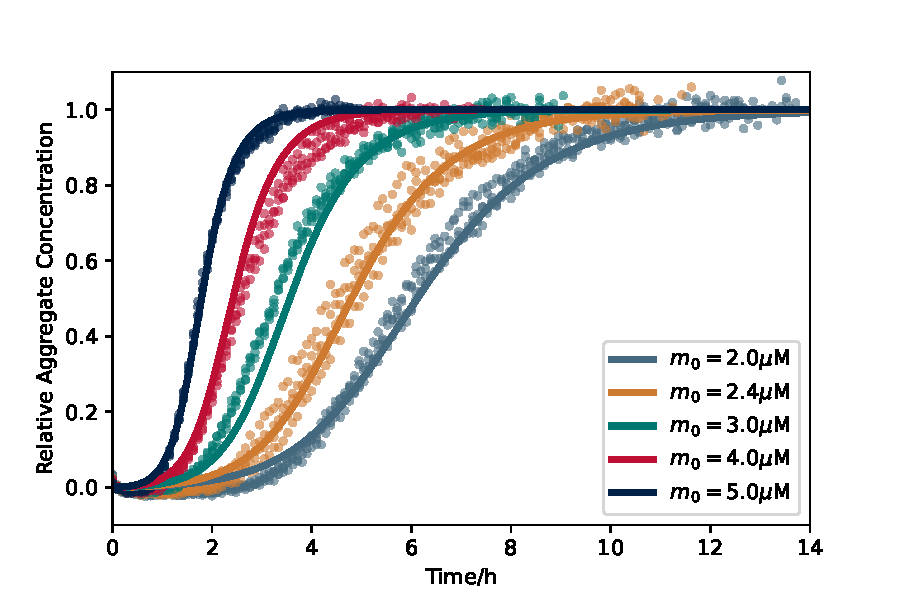
\includegraphics[width=0.8\textwidth]{figures/4-agg-figs/invitroDemo.pdf}
    \caption{Fitting in vitro aggregation data. The rate constants have been fit globally. We set $\nc=2$, $n_2=2$ and fit $k_on k_2=5.60\times10^{16}$ and $k_on k_n=9.992\times10^{8}$}. Fitting has been done using \textit{AmyloFit} software \cite{meisl_molecular_2016}. Data taken from \cite{cohen_proliferation_2013}.
    \label{fig:4-invitro}
\end{figure}

\todo{Mention how we can actually get the aggregation data perhaps?} Typical aggregation have an initial exponential increase in aggregate concentration due to the secondary nucleation process. As the monomer concentration is depleted the rate of aggreagtion slows until all the monomer is aggregated. The secondary nucleation step is autocatalytic as aggregates speed up the formation of more aggregates leading to a postive feedback and fast transition from mostly monomer to mostly aggregate.\todo{Discussion of scaling, typical length, etc., could actually also plot M/P, but just generally could have a bit more discussion here.}

\subsection{Failure to Recapitulate Disease}

The aggregation curves in test tube experiments are well understood by the reaction kinetics, but lack many crucial features of the development of neurodegenerative disease in living systems. Specifically, the model in (\ref{eq:4-Mvitro})-(\ref{eq:4-mvitro}) does recapitulate the discrete seeding transition, observed recovery of mice following treatment, or explain why the disease typically occurs in later life. These observations and the contradiction with the in vitro model are outlined below.

\subsubsection{Discrete seeding transition to disease}

In some model systems of neurodegenerative diseases, aggregation is only observed when the tissue or cells are seeded \cite{miller_tau_2021, tuck_cholesterol_2022}. For example, pathological aggregates are only observed in hippocampal slice cultures from P301S tau transgenic mice when the system is exposed to a high concentration of preformed assemblies at some earlier time (seeding) \cite{miller_tau_2021}. Small doses of tau assemblies do not increase aggregate concentration when compared to an unseeded system. However, for large doses of tau assemblies, the observed aggregate concentration was increased (and further increased when the dose was increased again). This phenomena is well established \cite{jucker_propagation_2018} and has been used to develop reporter lines assays to determine the presence of aggregates.\todo{cite the reporter}

The in vitro dynamics cannot explain this phenomena. The in vitro early time aggregation is dominated by an exponential growth, from the secondary nucleation process, $M(t) = M_0\exp(k_2 m_0^{n_2}t)$ where $M_0$ is the aggregate population at time $t=0$. Thus, addition of a seeding mass of aggregates, $M_S$, would correspond to shifting the aggregation process in time, but would not cause this transition between a stable and unstable system at some non-zero seeding.

% At early time in the in vitro dynamics, the aggreagtes proliferate exponentially. Thus, an injection of seed concentration acts to speed up this aggreagation process and can lead to much highe concntrations. However, this cannot describe the situation in all systems, as the . Additionally, when the seed concentration is varied, this exponential hypothesis would predict that the observed aggregate


% An existing hypothesis surrounding the onset of diseases from protein aggregation are built around the early time exponential growth of the disease. Specifically, that 
% The exponential growth hypothesis predicts that aggregate mass increases exponentially in time
% \begin{equation}
%     M(t) = S\exp{\kappa t}
% \end{equation}
% where $S$ is the aggregate mass at time $t=0$. In a seeded system, we typically expect the seeded aggregate mass to be much greater than the natural mass of aggregates and so we approximate $S$ as the mass of seeds.

% Consider three identical systems, seeded with different initial concentrations of the aggregated proteins; $S_1$, $S_2$, and $S_3$. The systems will aggregate and at some threshold, $M_D$, we will detect the aggregates in the cell. The exponential growth hypothesis can be used to identify growth rates. We identify the first time that aggregates are seen at as $t_i$ for a system seeded with $S_i$ aggregates. Then the growth rate, $\lambda$, is given by
% \begin{equation}
%     \lambda = \frac{\ln(S_1)-\ln(S_2)}{t_2-t_1}
% \end{equation}
% Therefore an experiment that does not satisfy this
\subsubsection{Explaining and Informing Treatments}

Currently the leading therapeutics for neurodegenerative diseases are based on immune therapies, such as monoclonal antibody therapies. In these treatments, antibodies bind to pathological fibrils to either disrupt the toxicity, or identify the structures for destruction via immune processes \cite{wisniewski_immunotherapeutic_2015, berg_biochemistry_2002}. \todo{list some current therapies?} These processes do not occur in test tubes and so cannot be described or explored by in vitro models.

More recently, short, synthetic, single-stranded DNA or RNA molecules, called antisense oligonucleotides (ASOs) are being explored as therapeutic candidates to treat NDDs \cite{rinaldi_antisense_2018}. The ASOs bind to target mRNA and thus limit transcription, reducing the expression of the aggregating monomer protein. In multiple studies, injections of ASOs were able to reduce the monomeric protein and this led to reduction and even removal of aggregates in the brain \cite{cole_-synuclein_2021, devos_tau_2017, mummery_tau-targeting_2023}. These studies demonstrate the enormous clinical potential of ASOs that target tau and $\alpha$-synuclein, two aggregating proteins associated with PD and AD. This presents a major opportunity to develop effective treatments for NDDs.

However, in order to realise these therapeutic opportunities, it is necessary to understand the different processes that affect the development of the disease in living cells and tissues. Test tube experiments show an inevitable conversion of monomer into aggregates, and cannot recapitulate the behaviour responsible for the reduction of aggregates and associated recovery of brain function in treated mice \cite{cole_-synuclein_2021}. Furthermore, developing a quantitative theory that can describe the onset and progression of disease will resolve the size of effects required for an intervention to have a meaningful change in prognosis.

\subsubsection{Long timescale in disease}\label{subsubsec:onsetage}

Test tube aggregation kinetics provide estimations for typical aggregation parameters and timescales. Typical aggregation experiments, such as those shown in Figure \ref{fig:4-invitro}, approach completion after around 10 hours, and have a doubling time of around an hour during the early exponential growth phase \cite{meisl_mechanistic_2022}. However, this understanding does not translate to the onset of disease in human populations. Around one in ten adults over the age of 65 have AD, increasing to four in every ten adults over 95 \cite{hou_ageing_2019}. This late age of onset is also seen for PD and ALS, with only $4\%$ of PD cases being under the age of 50 and the incidence increasing by a factor of $5$–$10$ from cases in their fifties to eighties \cite{van_den_eeden_incidence_2003, poewe_parkinson_2017}. This disparity of five orders of magnitude (one hour to one decade) clearly shows that something is missing from the current mechanistic models mapping in vitro protein aggregation kinetics onto the development of disease. In this chapter I will identify processes that are missing in vitro and develop a model to include all of these competing mechanisms. I will then demonstrate how these models can explain previously inexplicable observations and the consequences for the design of rational therapeutics.

\section{Aggregation Kinetics in vivo}

In living systems, there are additional processes in the `life cycle' of a protein. Specifically, how proteins are manufactured and removed. Many proteins that aggregate during disease are functional, for example \todo{specifics}. As such, we expect the concentration of these proteins will be maintained as part of homeostasis and thus in vivo the monomer concentration is constant, $m(t)=m_0$. In order to maintain the monomer concentration precisely, the cellular production and removal will need to be much faster than the aggregation kinetics and thus we write this as
\begin{equation}
    \frac{\text{d}m}{\text{d}t} = \epsilon^{-1}\left( \gamma - \lambda_1 m \right) + \text{aggregation kinetics}
    \label{eq:4-minvivo}
\end{equation}
where $\gamma$ and $\lambda_1$ are scaled rate constants for production and removal of the monomer respectively and $\epsilon$ is a small parameter that separates the timescales. The leading order solution to (\ref{eq:4-minvivo}) is $m=\gamma/\lambda_1$ which sets $m_0$. In the subsequent analysis we only consider this leading order behaviour. A full solution as an expansion of $\epsilon$ could be explored, however the leading order behaviour is sufficient to capture key features of the disease.

In living systems aggregates can also be removed via active processes in the cells or surrounding tissue. Examples of such processes include \todo{give examples}. This changes the master equation to
\begin{equation}
\begin{split}
    \frac{\text{d}p_i}{\text{d}t} &= \delta_{i, n_C}k_n m^{n_C} + \delta_{i, n_2} k_2 m^{n_2} \left(\sum_{j=\nc}^{\infty} j p_j\right) + 2k_\text{on} m (p_{i-1}-p_i) + 2k_{off} (p_{i+1}-p_i) - \lambda_i(p_i),
    \end{split}
    \label{eq:4-pi_cleared}
\end{equation}
where $\lambda_i(p_i)$ is the clearance rate for aggregates of each size.

\subsection{Unbounded Clearance}

The exact mechanisms of clearance and their kinetics remain unknown in many living systems. In the spirit of Occam's (or informally OCIAM's) razor we begin by considering the simplest kinetics: the clearance rate is proportional to the number of aggregates and independent of size $\lambda_i(p_i)=\lambda \times p_i$. We begin by analysing this system to demonstrate the inability to recapitulate all observed experimental results and to build an analysis framework for other systems.


The moment equations now define a linear system, since $m=m_0$ is constant, and so we can define $\textbf{q}=(P, M)^\text{T}$ and the evolution of the system becomes
\begin{equation}
    \dot{\textbf{q}} =
    \underbrace{\left(
    \begin{array}{cc}
    -\lambda & k_2 m_0^{n_2} \\
    2 k_\text{on}m_0 & n_2 k_2 m_0^{n_2}-\lambda  \\
    \end{array}
    \right)}
    _{\textbf{A}}
    \textbf{q}
    +
    \underbrace{\left(
    \begin{array}{c}
    k_n m_0^{\nc} \\
    \nc k_n m_0^{\nc} \\
    \end{array}
    \right)}
    _{\textbf{b}}
    \label{eq:4-momentEvomatform}
\end{equation}
where the dot indicates the time derivative and we've defined the matrix $\textbf{A}$ and vector ${\textbf{b}}$ in the equation. The solution is 
\begin{equation}
    \textbf{q} = -\textbf{A}^{-1}\textbf{b}+\left(\textbf{q}_0+\textbf{A}^{-1}\textbf{b}\right)e^{\textbf{A}t}
    \label{eq:4-momentSolvematform}
\end{equation}
where $\textbf{q}_0$ is a vector of the initial aggregate number and aggregate mass concentration. The steady state behaviour is determined by the eigenvalues of $\textbf{A}$, which are
\begin{equation}
    \nu_{\pm} = \frac{1}{2} \left(k_2 m_0^{n_2} n_2 \pm \sqrt{8 k_\text{on} m_0 k_2 m_0^{n_2} + \left(n_2 k_2 m_0^{n_2}\right)^2} - 2 \lambda \right).
    \label{eq:4-A_eig}
\end{equation}
The system always has $\nu_{-} \leq 0$, however the sign of $\nu_+$ depends on the the clearance constant, $\lambda$. If $\nu_+>0$, then the system has no steady state and both the mass and number of aggregates has unbound growth. For $\nu_+<0$ then there exists a steady state solution for $t\rightarrow\infty$, $\textbf{q}_\infty = -\textbf{A}^{-1}\textbf{b}$. The stability of the system is independent of the primary nucleation rate as there is no positive feedback on the production of aggregates, however this nucleation process still affects the steady state aggregate mass. Given a set of rate constants we can therefore define a \textit{critical clearance}, $\lambda_{\text{crit}}$, that determines whether the aggregation will be bound. Solving equation (\ref{eq:4-A_eig}) for $\nu_+=0$ gives
\begin{equation}
    \lambda_{\text{crit}} = \frac{1}{2} \left(k_2 m_0^{n_2} n_2 + \sqrt{8 k_\text{on} m_0 k_2 m_0^{n_2} + \left(n_2 k_2 m_0^{n_2}\right)^2}\right).
    \label{eq:2-critclear}
\end{equation}
\todo{check this critical value} When $\lambda>\lambda_{\text{crit}}$ the system approaches a steady state and when $\lambda<\lambda_{\text{crit}}$ the mass of aggregates grows exponentially as $M(t)\sim M(0)e^{\nu_+ t}$.

Alternatively, we could fix the clearance rate and determine the maximum monomer concentration, $m_0$, that leads to a steady state solution. The stability condition is
\begin{equation}
    -2 k_2 k_\text{on} m_0^{n_2+1} - n_2 k_2 \lambda m_0^{n_2} +\lambda^2 = 0
    \label{eq:2-critmon}
\end{equation}
which has exactly one positive solution that defines the critical monomer concentration $m_0^{(crit)}$. At monomer concentrations above $m_0^{(crit)}$ the system has unbound aggregation and below $m_0^{(crit)}$ the aggregate mass approaches a steady state. This is a useful perspective as the new treatment technologies, such as ASO/CHARM treatments can vary $m_0$ as a therapeutic strategy, however currently no theoretical description exists to capture this.

At the steady state, $\textbf{q}$ is constant, and so we can determine the average aggregate length as the ratio of the aggregate mass and aggregate number, $\bar{l}=P/M$. At the steady state this will be constant
\begin{equation}
    \bar{l}^* = \frac{M^*}{P^*} = \frac{2 k_\text{on} m_0 + \nc \lambda_{\text{crit}}}{\lambda_{\text{crit}}+(\nc-n_2)k_2 m_0^{n_2}}.
    \label{eq:4-lbarConstClear}
\end{equation}
The effect of secondary nucleation on the average length initially seems confusing, and in particular it might seem strange that the dependence on $k_2$ vanishes when $\nc=n_2$. This can be explained as aggregates are only nucleated at length $\nc$ or $n_2$ and the population of aggregates at other lengths decays geometrically away from these source terms. When $\nc = n_2$ there is only one source term, therefore the average aggregate length is determined entirely by the rate of decay of the aggregate population with increasing length. If the nucleation rate were increased, the population at length $n_c$ would increase, and subsequently the population of aggregates of every length would increase proportionally, however the decay length would remain the same and the \textit{average} aggregate length would also be unchanged. For $n_2>\nc$ the source term at $n_2$ increases the aggregate population at large lengths and so increases the average length.

\subsubsection{Exactly Solving the Full Linear System}

When the system clears aggregates at a linear rate we can calculate the steady state aggregate length distribution as well as the time evolution of an arbitrary number of moments of this distribution.

Additionally, we can determine the time full evolution of any initial distribution in the moment space. Since this is a linear system, the we can take an arbitrary number of moments. Define
\begin{equation}
    Q^{N} = \sum_{\nc}^\infty i^N p_i
\end{equation}
which has the time evolution
\begin{equation}
\begin{split}
    \frac{\text{d}Q^{N}}{\text{d}t} &= \sum_{\nc}^\infty i^N \left( \delta_{i, n_C}k_n m^{n_C} + \delta_{i, n_2} k_2 m^{n_2} M + 2k_\text{on} m (p_{i-1}-p_i) + 2k_{off} (p_{i+1}-p_i) - \lambda p_i \right) \\
    \frac{\text{d}Q^{N}}{\text{d}t} &= \sum_{\nc}^\infty i^N \left( \delta_{i, n_C}k_n m^{n_C} + \delta_{i, n_2} k_2 m^{n_2} M + 2k_\text{on} m (p_{i-1}-p_i) - \lambda p_i \right) \\
    &=n_C^N k_n m^{n_C} + n_2^N k_2 m^{n_2} M + \sum_{\tau=0}^{N-1} 2k_\text{on} m \binom{N}{\tau} Q^{\tau} - \lambda Q^{N}.
\end{split}
\end{equation}
Since the evolution of a moment only depends on itself, or moments of lower order moments, we can still solve the system equation (\ref{eq:4-momentEvomatform}).

It is also possible to find $p_i$ for the steady state. Assume $n_c=n_2$. In steady state the concentration of each aggregate size is in detailed balance so for the smallest aggregates, of length $n_c$, we have
\begin{equation}
    k_n m_0^{\nc} + k_2 m_0^{\nc} M - 2 k_\text{on} m_0 p_{\nc} - \lambda p_{\nc} = 0
    \label{mpnc1}
\end{equation}
and detailed balance for all aggregates of other lengths gives
\begin{equation}
    (2k_\text{on} m_0 + \lambda)p_{i+1} = 2k_\text{on} m_0 p_i.
\end{equation}
This is solved by
\begin{equation}
    p_i = \alpha^{i-\nc} p_{\nc}\quad\text{ with }\quad\alpha=\frac{2k_\text{on} m_0}{2k_\text{on} m_0 + \lambda}
\end{equation}
and so we get another equation connecting $M$ and $p_{\nc}$, that is
\begin{equation}
    M = \sum_{i=\nc}^{\infty}i\alpha^{i-\nc} p_{\nc} = p_{\nc}\left( \frac{(\lambda +2k_\text{on} m_0) (2 k_\text{on} m_0 + \lambda  \nc)}{\lambda^2} \right).
    \label{mpnc2}
\end{equation}
Combining equations (\ref{mpnc1}) and (\ref{mpnc2}) gives the same mass, $M$, as before and 
\begin{equation}
    p_{\nc} = \frac{\lambda^2 k_n m_0^{\nc} }{(2 k_\text{on} m_0+\lambda \nc) \left(\lambda ^2-k_2 m_0^{\nc} (2 k_\text{on} m_0+\lambda  \nc)\right)}
\end{equation}
which for realistic signs of the parameters (e.g. no negative clearance) gives the critical behaviour at the same values as before. \todo{need to watch the bound for the $k_{off}$ term!}

Moving from the master equation to the moment description of the kinetics, we have assumed \todo{SC III: what assumptions have we made?}. Numerical simulation of the dynamics of the system at the level of the master equation can verify that the coarse grained description provides an accurate summary and prediction of the kinetics. In the most general case however, this presents computational challenges, as there is no upper limit on the aggregate length. Here, we introduce a maximum aggregate length that does not elongate but is still removed via the clearance mechanisms. The maximum length should be significantly larger than the mean length distribution and we can additional ensure that it is larger than lowest length populated by one aggregate, using equation \todo{get the equation in}. We then evolve this system using a \todo{fouth order Runge–Kutta method} to simulate the evolution of the full population distribution of aggregates of different lengths. \todo{Shows good agreement etc.?}

\begin{figure}
    \centering
    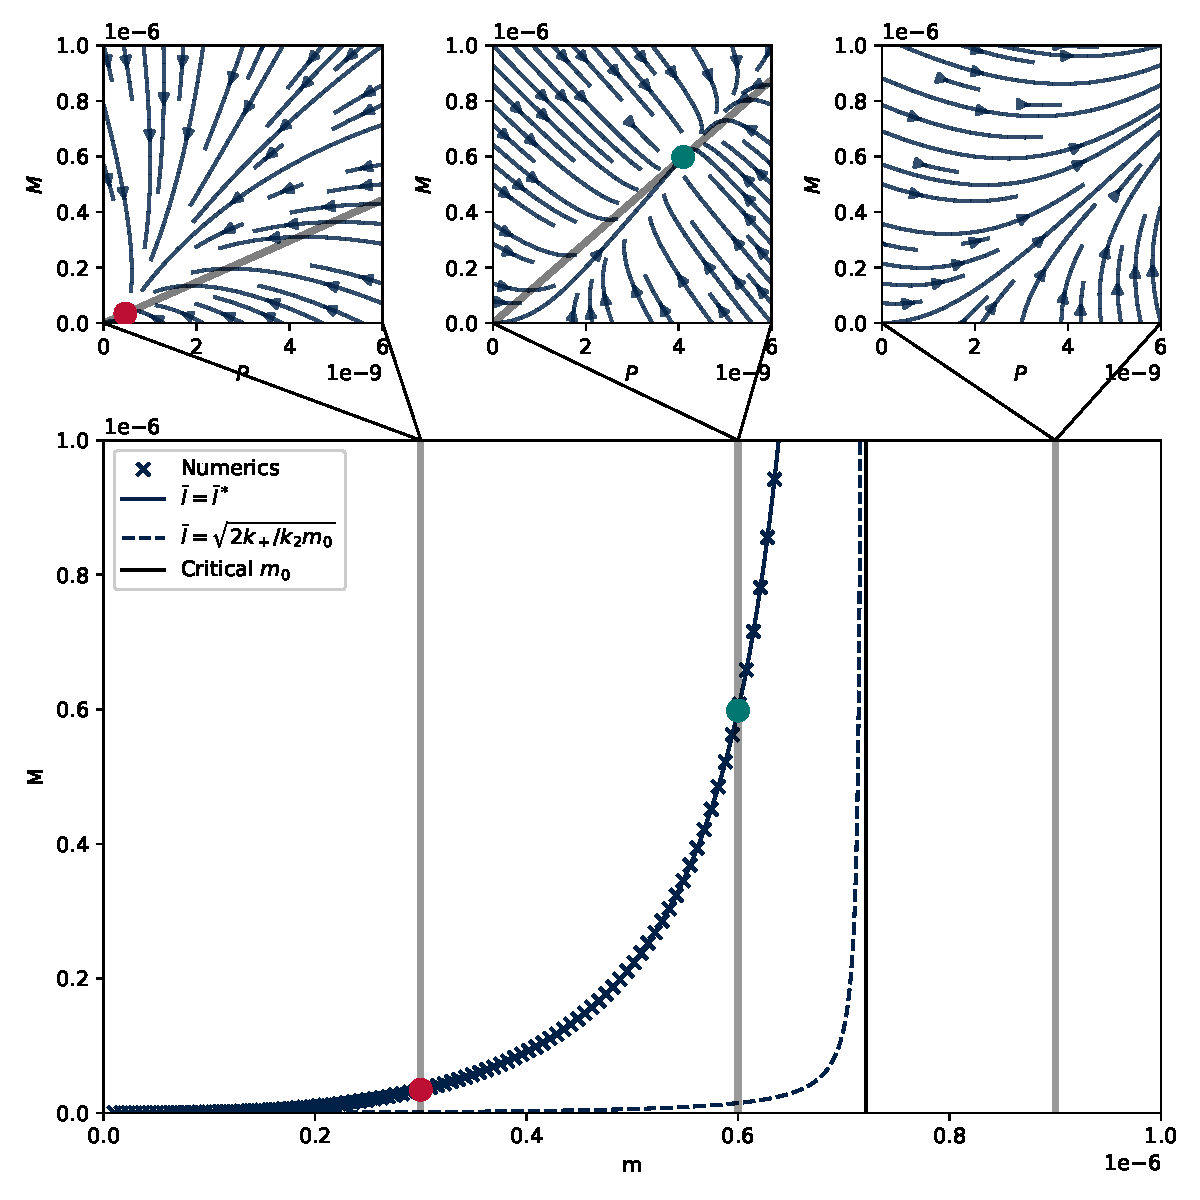
\includegraphics[width=0.8\textwidth]{figures/4-agg-figs/propClearSummary.pdf}
    \caption{Comparison of the different descriptions of the system, its flow and stability.}
    \label{fig:4-steadyConstClear}
\end{figure}

\subsection{Bounded Clearance}\label{subsec:4-boundedclearance}

The proportional clearance described above permits an analytically solvable model that gives insight into the role of clearance in neurodegenerative diseases. However the proportional clearance is an unphysical description for the removal of aggregates in all scenarios. Breaking down aggregates into the clearance products will require energy to break the bonds \todo{specify the bond} that connect the monomers and so the energy consumption rate will increase linearly with the rate of mass clearance. There will be some maximum energy consumption rate for the cell and this will therefore translate to a maximum clearance rate of aggregates. In this section we explore to fundamentally different phenomena that arise from this bounded clearance.

The exact functional form describing the kinetics of aggregate clearance will determine how the clearance rate approaches this upper bound. For example, there could be a finite fuel component such as ATP that is depleted as that aggregates are cleared and limits the clearance rate, the aggregates may cause toxic damage to the cell and affect the efficiency of cellular processes or, as we will assume, the clearance mechanism has enzyme-like rate kinetics. Consider the ubiquitin (Ub)-proteasome system (UPS) that tags aggregates with Ub before the aggregates are unfolded and cleaved in the proteasome, or chaperone mediated autophagy (CMA) where chaperones delivered to lysosomes to be degraded \cite{ciechanover_degradation_2015} \todo{GM: Ulrich Hartl refs} Both of these clearance processes can be modelled as the binding of an essential clearance component (E), either Ub or the chaperone, before the bound complex is then removed from the system and the intermediary clearance component is released. For an aggregate $A_i$, with concentration $p_i$ and an clearance component $E$ with concentration $p_e$, the clearance reaction can be modelled as
\begin{equation}
        \ce{A_i + E <=>[$k_i^b$][$k_i^d$] C_i ->[$k^{c}_i$] E + Clearance Products} \label{eq:4-MM}
\end{equation}
where $k_i^b$ and $k_i^d$ are the binding and dissociation rates of the aggregate and intermediary component which and $k^{c}_i$ is the rate constant describing the removal of the aggregate. The intermediate clearance component binds to an aggregate of size $A_i$ to form a complex $C_i$, with concentration $c_i$, which can either dissociate or be broken down and cleared.

This setup is similar to the Michaelis–Menten (MM) description for reactions kinetics where the $E$ component is the enzyme. However here we have a series of different sized aggregates that all compete for the same component. We can calculate the expected rates in the system in the same way as the single substrate analysis: assume that the total $E$ component in the system is constant, $p_e^{T} = p_e + \sum_i c_i$, and that the aggregate binding is at equilibrium for all lengths, $k_i^b p_e p_i = k_i^d c_i$. These expressions give
\begin{equation}
    c_i = p_e^{T}\frac{k_i^b}{k_i^d}\left(\frac{p_i}{1+\sum_j p_j \frac{k_j^b}{k_j^d}}\right).
\end{equation}
The clearance of aggregates of size $i$ in the system is $\lambda_i = k_i^{c}c_i$. In general this will not reduce to a closed form pair of moment equations, however if we assume that the rates are independent of aggregate size, $k_i^{c}=k^{c}$, $k_i^{b}=k^{b}$ and $k_i^{d}=k^{d}$, then this reduces to the typical MM kinetics, as each all aggregates are effectively the same single substrate. This now gives the moment equations with modified clearance as
\begin{align}
    \frac{\text{d}M}{\text{d}t}&= \nc k_n m_0^{\nc} + n_2 k_2 m_0^{n_2} M + 2 k_\text{on} m_0 P - \frac{\lambda_M M}{K_M+P} \\
    \frac{\text{d}P}{\text{d}t}&= k_n m_0^{\nc} + k_2 m_0^{n_2} M - \frac{\lambda_{M} P}{K_M+P}.
    \label{eq:4-reducedMM}
\end{align}
where we have defined $\lambda_M = k^{c} p_e^T$ and $K_M = k^d/k^b$. When $P \ll K_M$, the clearance is proportional to the concentration as before, with an equivalent clearance rate of $\lambda = \lambda_M/K_M$. However for $P \gg K_M$, the clearance saturates with a maximum number clearance rate $\lambda_M$ and a maximum mass clearance rate mass clearance rate $\lambda_M\bar{l}$.

Solving for the steady state of the system, $\text{d}M/\text{d}t=\text{d}P/\text{d}t=0$, gives three pairs of solutions for $M^*$ and $P^*$. For typical system parameters, two pairs of the steady states have real positive solutions for both $M^*$ and $P^*$. At a critical monomer concentration these two solutions undergo a bifurcation and merge, such that for monomer concentrations above this critical value there no longer exists a positive steady state. Similarly to the case for proportional clearance, when the monomer concentration is large we expect the mass of aggregates in a system to exhibit unbound growth. When the monomer concentration is less than this critical value, there exists a steady state, however unlike when the clearance is proportional, the system will not necessarily converge to this equilibrium. Whether the steady state is reached depends on the initial mass and number concentrations ($M$ and $P$).

Again, we can solve for the steady state length distribution when this exists. For $\nc=n_2$ we have
\begin{equation}
    k_n m_0^{\nc} + k_2 m_0^{\nc} M - 2 k_\text{on} m_0 p_{\nc} - \frac{\lambda_P p_{\nc}}{K_M + P} = 0
\end{equation}
and detailed balance for all aggregates of other lengths gives the same geometric decay, but with a different decay rate, $\alpha$,
\begin{equation}
    p_i = \alpha^{\nc-i} p_{\nc}\quad\text{ with }\quad\alpha=\frac{2k_\text{on} m_0 (K_M + P)}{2k_\text{on} m_0 (K_M + P) + \lambda_P}.
\end{equation}
Evaluating the sums to determine $M$, $P$ and $p_{\nc}$, gives the same pair of positive real solutions, as expected.

\begin{figure}
    \centering
    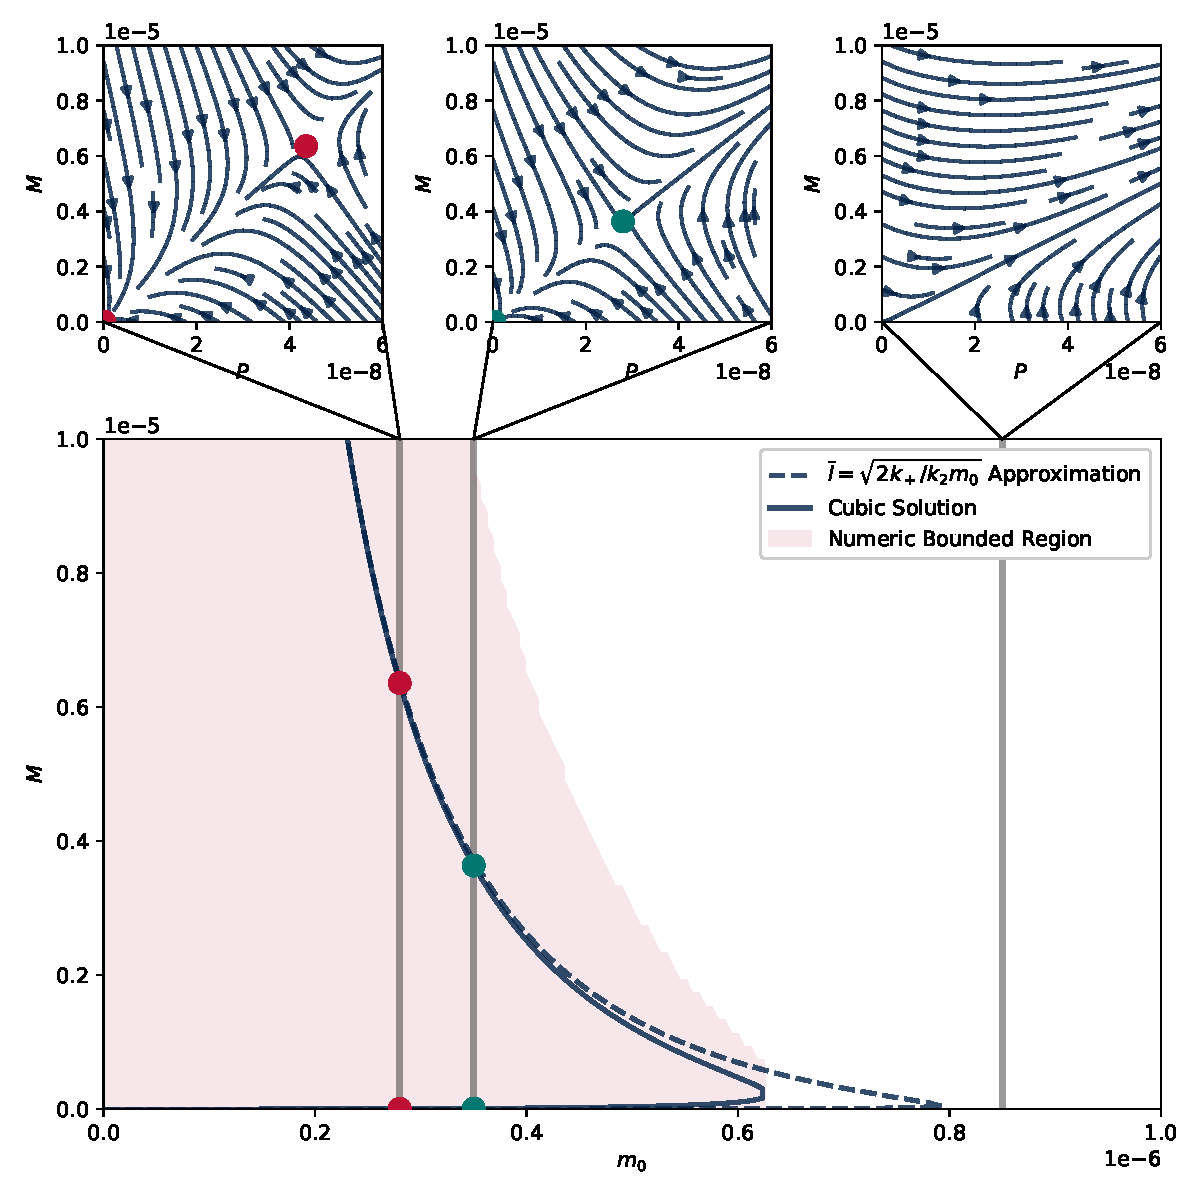
\includegraphics[width=0.8\textwidth]{figures/4-agg-figs/confusingNumericRegion.pdf}
    \caption{Comparison of the different descriptions of the system, its flow and stability.}
    \label{fig:4-steadyMM}
\end{figure}

\subsection{Reduced Models of in vivo Aggregation}

When the aggregate clearance and other rates are prescribed, the system and its dynamics are determined by three variables, $M$, $P$ and $m_0$, where $m_0$ is unaffected by the aggregation kinetics, however we keep this as a system variable to explore the role of monomer reducing therapies.

\subsubsection{Constant Clearance}

The fate of a system determines whether a cell is \textit{healthy} or \textit{diseased} with unbound growth describing the diseased state and a finite steady state for healthy cells. In the three parameter description, this will be entirely determined by the monomer concentration. We can further reduce the system to a two parameter description by prescribing the average length of the aggregates, $\bar{l}$. In the case of unbound proportional clearance, the steady state is given by $\mathbf{q}=\mathbf{A}^{-1}\mathbf{b}$ and so an obvious choice for $\bar{l}$ is to choose the steady state value, $\bar{l}^*=M^*/P^*$, equation (\ref{eq:4-lbarConstClear}), which exactly recovers the same steady state mass ($M^*$) as the full model. With this assumption, the moment equation for $M$ becomes
\begin{equation}
    \frac{\text{d}M}{\text{d}t}= \nc k_n m_0^{\nc} + n_2 k_2 m_0^{n_2} M + 2 k_\text{on} m_0 M/\bar{l}^* - \lambda M.
    \label{eq:4-reducedConstClear}
\end{equation}
Along with $\text{d}m_0/\text{d}t=0$ this defines a reduced model that captures the key features of the aggregation kinetics: the approach to the steady state for $m_0 < m_0^{\text{crit}}$ and unbound growth for $m_0 > m_0^{\text{crit}}$. A phase plane of this model clearly shows the dynamics and the emergence of the stability. When the aggregate mass is very low, the mass increases (flows upwards on the plot) until it approaches the steady state line and is balanced by clearance. When the monomer concentration is high ($m_0>m_0^{\text{crit}}$) there is no steady state distribution and so the aggregate mass will continue to increase. When the monomer concentration is low ($m_0<m_0^{\text{crit}}$) and the mass of aggregates is high, aggregates will be cleared from the system (move down on the phase plane) until the system reaches the steady state mass concentration.

% \begin{figure}
%     \centering
%     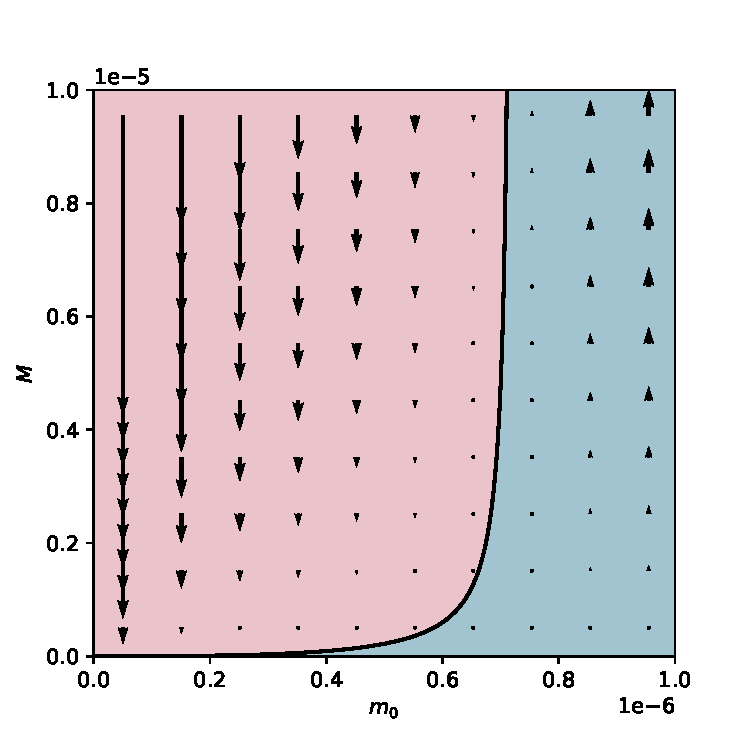
\includegraphics[width=0.8\textwidth]{figures/4-agg-figs/flowConstClear_nocol.pdf}
%     \caption{Flow for const clear.}
%     \label{fig:4-flowConstClear}
% \end{figure}
The average length assumption projects the two dimensional $M-P$ plane flows onto a line in $M-P$ space. Figure \todo{ref} shows this line and the key features of the dynamics are well captured by the projection onto the line. We assumed a linear relationship between $M$ and $P$, however a more complex functional relationship may capture the dynamics more accurately as there appears to an obvious slow manifold in the $M-P$ space, however the linear relationship captures the key features and makes it easy to interpret fixed points and their stability.

When the monomer concentration is high and the linear system grows unbound, the long time behaviour of $\mathbf{q}$ is determined by the eigenvector of $\mathbf{A}$ corresponding to the positive eigenvalue $\nu_+$. The ratio of the components of this eigenvalue gives the average length which is
\begin{equation}
    \bar{l} = \frac{m_0^{-\frac{n_2}{2}} \sqrt{k_2 n_2^2 m_0^{n_2}+8 k_\text{on} m_0}+\sqrt{k_2} n_2}{2 \sqrt{k_2}}.
\end{equation}
Typically, we expect $k_2 m_0^{n_2} \ll k_\text{on} m_0$ and thus $\bar{l} = m_0^{\frac{1-n_2}{2}}\sqrt{2 k_\text{on}/k_2}$. Using this $\bar{l}$ in the reduced dynamics, equation (\ref{eq:4-reducedConstClear}), predicts a much lower steady state mass (shown in Figure \ref{fig:4-steadyConstClear}), however both length distributions exactly capture the transition from the bound to unbound dynamics.
% The transition from unbounded growth to a finite steady state mass gives an expression for the critical clearance of a system. Alternatively, this transition can occur for a constant clearance that approaches a steady state if the monomer concentration is low, but grows unbound if the monomer concentration is high. Plotting the steady state mass, $M^*$, against the monomer concentration shows this transition. A system initialised with a total mass below the steady state mass, $M_0 < M^*$ will increase to $M^*$ and a system with $M_0 > M^*$ will decrease to $M^*$. When $M^*$ does not exist then the mass increasess without bound. To visualise this we assume that the number concentration is enslaved to the mass distribution, to give $P=M/\bar{l}$ even when the system has not equilibrated. This reduces the dynamics to be a function of $M$ and $m_0$ only and gives a two-dimensional phase plane of the system in this space and visualise the flows, as show in \todo{figure}. The app
\begin{figure}
    \centering
    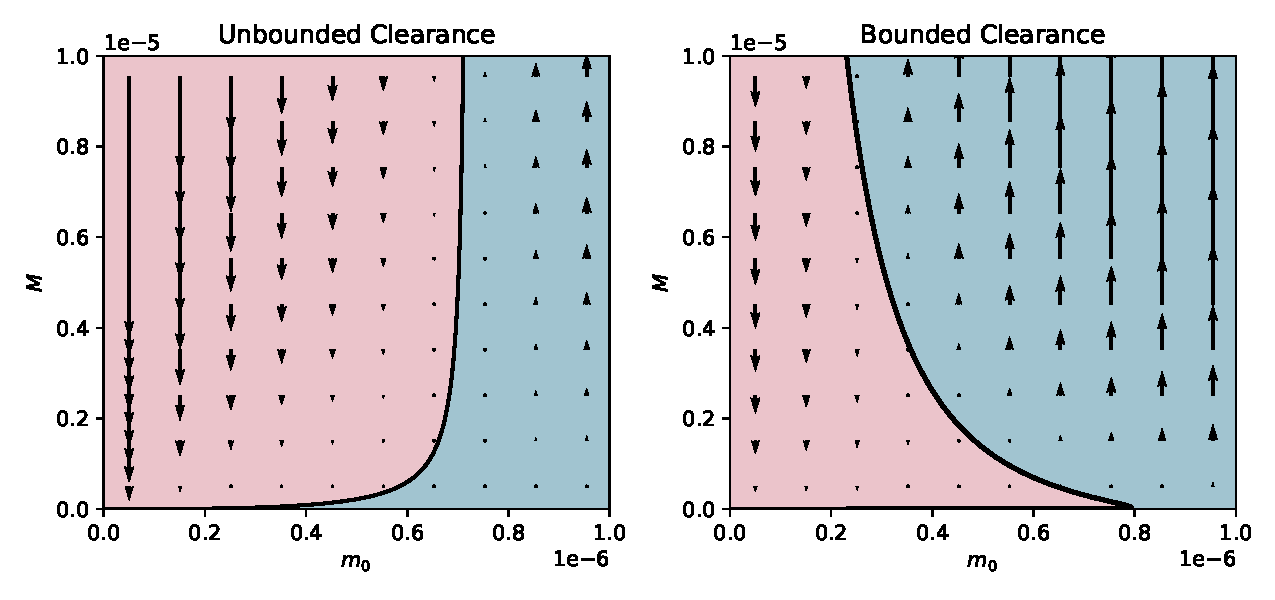
\includegraphics[width=0.95\textwidth]{figures/4-agg-figs/reduced_nocol.pdf}
    \caption{Flow for MM P.}
    \label{fig:4-flowMM_P}
\end{figure}

\subsubsection{Bound Clearance}

Similarly for the case of a bounded clearance, we reduce the model to a two parameter description by assuming a value of the  $\bar{l} = \sqrt{2 k_\text{on}/k_2 m_0}$ and $P=M/\bar{l}$.\todo{this is the eigenvalue of the exponentially growing mode!} The fixed points of this reduced system are now quadratic in $M$ and this gives two steady states when $m_0$ is low and no steady states when $m_0$ is high. This reduced model captures the key features of the full model, with the existence of a stable and unstable fixed point and a critical monomer concentration. However, the exact value at which this bifurcation occurs is different in the full and reduced models. This is due to the approximation for $\bar{l}$ being accurate for large steady state mass is large, which is the upper branch of the stability line at low monomer concentration. Fig \todo{which fig} shows that the two models agree in this region.

The fate of the system now depends on both the monomer concentration and the aggregate mass. The system is only stable, and therefore healthy, if both the monomer concentration and aggregate mass is low. Intuitively this dependence on the aggregate mass makes sense. If there are more aggregates (number and mass) in the system, then the rates of secondary nucleation and elongation will increase. When the aggregate clearance rate is high enough to out compete these effects then the aggregate mass/number is reduced and approaches a steady state value where the production of aggregates and clearance rates are balanced. For very large aggregate mass/number, the production rates of aggregates continue to increase with increasing aggregate mass/number, however for physically realistic models of clearance mechanisms the removal rate of aggregates will begin to saturate and at some point will no longer be able to balance the aggregate production/elongation rates, leading to runaway aggregation.

% \begin{figure}
%     \centering
%     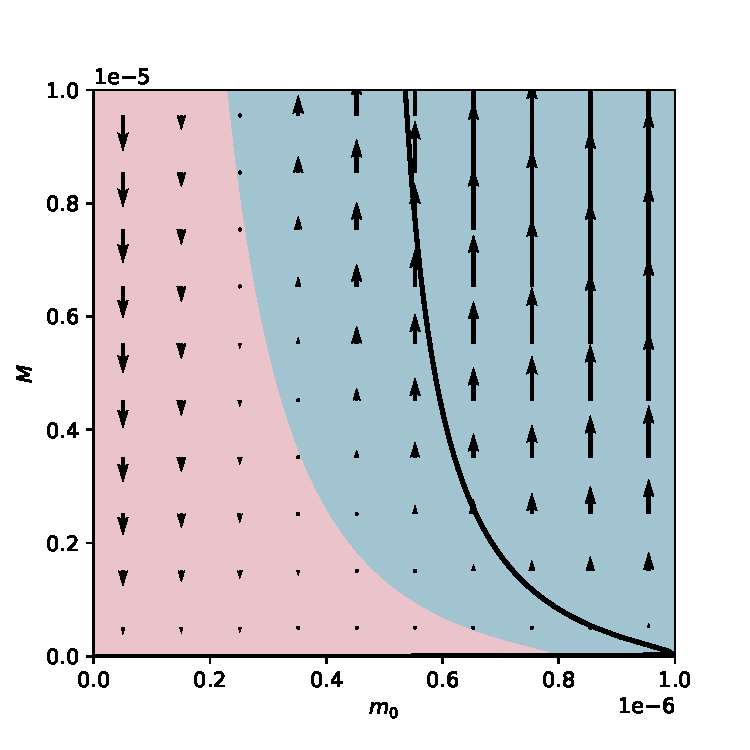
\includegraphics[width=0.8\textwidth]{figures/4-agg-figs/flowMM_nocol.pdf}
%     \caption{Flow for MM P.}
%     \label{fig:4-flowMM_P}
% \end{figure}

\section{Generalising the Dynamics}

\subsection{Generalised Models of Clearance}

When developing the model of bounded clearance in section \ref{subsec:4-boundedclearance} we focused on the kinetics of an enzyme-like mediated clearance mechanisms with binding rates independent of aggregate size. Crucially, this model predicts an upper unstable branch in the phase plane of the $M-m_0$ dynamics. However, this phenomena is general to any clearance that increases sub linearly with increasing aggregates. Since the aggregate production rate from nucleation is proportional to the mass of aggregates, any sub linear clearance will not be able to compete at large aggregate mass concentrations. For example, if the intermediary clearance component ($E$) can attach to aggregates at any position, then we would expect this binding rate to be proportional to the aggregate length and the dissociation to be remain constant, so that ${k_i^b}/{k_i^d}\sim i$. It also makes sense that the clearance processes, such as those from the proteasome system, will breakdown aggregates at a rate proportional to the number of monomer-monomer bonds that have have to be broken, $\sim(i-1)$, and so we can approximate $k_i^{c} \sim i^{-1}$. With these modifications, the clearance rate now saturates in $M$, rather than $P$ giving clearance for the number and mass concentrations as $\Tilde{\lambda}P/(\Tilde{K}+M)$ and $\Tilde{\lambda}M/(\Tilde{K}+M)$ respectively. When the rate constants $\Tilde{\lambda}$ and $(\Tilde{K})$ are scaled by a constant of the order of the average length, the system has identical behaviour to the number saturating clearance, although the exact fixed points are slightly perturbed. The reduced dynamics for this model is shown in the first panel of Figure \ref{fig:4-generalReduced}.

We expect that the complex regulation of living systems will result in multiple mechanism to remove aggregates, with different kinetics and saturation. Again as long as the removal mechanisms are sublinear in mass, then the upper unstable branch mass will be bistable and the key features of the model remain. For example, combining a clearance proportional to mass and an MM-like clearance that saturates in aggregate number (the clearance mechanisms in equations (\ref{eq:4-reducedConstClear}) and(\ref{eq:4-reducedMM})) we find that the bifurcation point moves to a higher monomer concentration, but that the bifurcation structure remains almost unchanged, as can be seen in \todo{one of the panels} of Figure \ref{fig:4-generalReduced}.

\begin{figure}
    \centering
    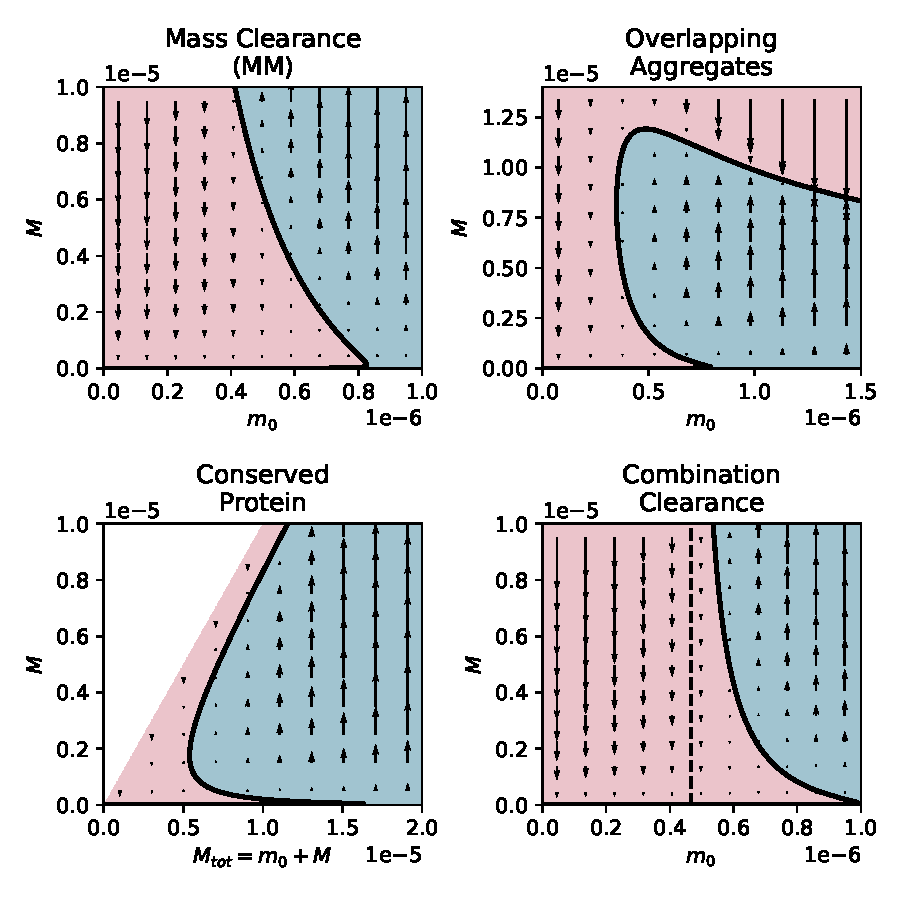
\includegraphics[width=0.95\textwidth]{figures/4-agg-figs/generalisingReduced_nocol.pdf}
    \caption{General reduced dynamics.}
    \label{fig:4-generalReduced}
\end{figure}

\subsection{Exponential Growth is Unphysical}

The exponential growth of the aggregate mass is labelled as the disease state. For a cell of finite volume and resources the exponential growth can only occur for finite time before other factors reduce the rate of growth. To describe this, we can modify the reduced model in equation \ref{eq:4-reducedMM} and introduce a correction to the secondary nucleation. As the aggregate concentration increases, multiple aggregates may touch or overlap in space and thus prevent this overlapping region of the aggregate surface from acting as a catalyst for secondary nucleation. We expect the overlapping region to increase like $M^2$ and so the aggregation kinetics with this corrected aggregate surface becomes
\begin{equation}
\frac{\text{d}M}{\text{d}t}= \nc k_n m_0^{\nc} + n_2 k_2 m_0^{n_2} (M- \rho M^2) + 2 k_\text{on} m_0 M/\bar{l} - \frac{\lambda_M M}{K_M+M/\bar{l}}
\end{equation}
where $\rho$ is the overlap constant. Figure \ref{fig:4-generalReduced} \todo{some panel} shows the reduced dynamics as before, however there is now a hysteresis loop. For very low monomer concentration there is only one steady state as the clearance mechanisms grow faster than the secondary nucleation and the steady state is determined by the balance of primary nucleation and clearance. For intermediate monomer concentrations, there is a region where the secondary nucleation dominates, as before, however additionally for larger aggregate mass the crowding effects prevent further increase in aggregate mass and there is a third steady state that is stable with large aggregate mass. For even larger values of aggregate mass, the system undergoes the same bifurcation as before for low values of the aggregate mass, but this large aggregate mass steady state persists and is attracting everywhere. Phenomenological, we interpret this exactly as before, however now the aggregate mass in the diseased state is bound at some very high aggregate mass, which is more physical. Despite being bound, we expect that this large aggregate mass will still be toxic and thus is associated with the same pathology.


The models of aggregation considered so far assume constant monomer concentration in the cell, motivated by cellular homeostasis maintaining regulating this concentration. When the aggregate mass is large in the system the rate of aggregation will become increasingly fast and at some point will be on the same timescales as the regulation of monomer and so we cannot model the monomer as constant. An alternative is to assume the aggregation kinetics are much faster than the expression of the monomer and so the total protein in the system, $M_{tot} = M + m_0$ is constant. Assuming the MM-like clearance mechanism, the rate of change of aggregate mass is still given by equation (\ref{eq:4-reducedMM}) and substituting $m_0=M_{tot}-M$, so that $\dot{M}=-\dot{m_0}$. Physically, this corresponds to clearance mechanisms converting the aggregated mass back into monomer to conserve total protein. The dynamics of the new reduced model can be seen in a phase plane of $M$ and $M_{tot}$, this is shown in \todo{a panel of} Figure \ref{fig:4-generalReduced}.

Since $\dot{M}=-\dot{m_0}$, the effects of the conserved total protein will be seen when the aggregate mass concentration is the same order of magnitude as the monomer concentration. \todo{actually, we should think about this a bit more} There is also a region of the graph that is unfeasible, corresponding to there being more aggregated protein than there is total protein, which is not possible.  We therefore chose rate constants that show the effects of the bounded clearance on a similar scale to the aggregate mass. From the plot it can be seen that system dynamics for conserved total protein has the similar structure as the saturating secondary nucleation, except with an increasing upper branch. The upper branch for large monomer concentration has almost all protein in the aggregated state, however there still exists some monomer so that the nucleation rates balance the clearance rates. As with the saturating secondary nucleation, the seeding, monomer dependence and effects of clearance are all phenomenological the same in this modified model compared to the original reduced model in equation (\ref{eq:4-reducedMM}).

This model and the model in equation (\ref{eq:4-reducedMM}) represent two distinct regimes: the aggregation kinetics are much fast than the homeostatic mechanisms or the inverse. The full system is likely to couple these timescales, and neither $\dot{m_0} \neq 0$ nor $\dot{M}_{tot} \neq 0$ so that the arrows in the reduced models will not longer be vertical, but will be tilted. It is harder to determine the fate of the system from the coupled dynamics, but looking the two limiting regimes we recover the same macroscopic behaviour consistent with seeding, monomer reduction therapies and the transitions to disease via reduced clearance.

\subsection{Length Dependent Seeding}

In coarse gaining the system dynamics to the $m_0-M$ space we ignored the dependence of the fate of the system on $P$. Looking at the top row of Figure \ref{fig:4-steadyMM}, we can see that for a constant initial mass, the number of aggregates can determine whether the system evolves to an unbound aggregate mass or the low aggregate mass steady state. In fact, there exists maximum number of aggregates for which the aggregates mass will remain bound and if there are initially more aggregates in the system than this, then the flow of the system will be towards the state of infinite aggregates. This result is useful to understand seeding experiments in vivo. An experimental challenge is to control the length distribution of aggregates that will be used to seed a system to investigate the in vivo dynamics. Here we see that a different length distribution can in fact alter the fate of identical cells and so conclusions drawn from comparing the aggregation kinetics with uncontrolled length distributions may be misleading.

\todo{actually this could be interesting because if, for example longer agregates diffuse more slowly, then overall number could become dependent... nice to connect to, for example Georgia's spreading? could think about extensions inspired by the kind of model in \cite{agudo-canalejo_cooperatively_2020}.}

\subsection{Length Dependent Clearance}

Another physically motivated modification to the constant clearance model is to reduce the rate of clearance for longer aggregates. We expect longer aggregates will take longer to clear from living cells and tissue as there are more bonds to break. It is useful to understand if this will recapitulate the observed seeding behaviour, that is, whether a sudden increase in the concentration of longer, more persistent fibrils would cause a transition to exponential growth. The logic of this argument is that since the longer aggregates take more time to clear, that by the time they are removed from the system, the increase in secondary nucleation and subsequent elongation will have already replenished and then increased the concentration of longer aggregates, leading to positive feedback.

As we expect the clearance to be proportional to number of bonds, which goes like aggregate length, we assume $\lambda_i = \lambda i^{nu} p_i$, where we choose $\nu=1$. For the non-fragmenting, non-depolymerising system discussed here, the master equation for this model 
\begin{equation}
    \frac{\text{d}p_i}{\text{d}t} = \delta_{i, n_C}k_n m^{n_C} + \delta_{i, n_2} k_2 m^{n_2} \left(\sum_{j=\nc}^{\infty} j p_j\right) + 2k_\text{on} m (p_{i-1}-p_i) - \lambda i^{-1} p_i.
    \label{eq:4-pi_evolution}
\end{equation}
Unlike the previous clearance models, summing over the aggregate population at each length introduces a dependence on the $-1^\text{th}$ moment, $Q^{-1}=\sum_i i^{-1}$, for the evolution of the aggregate number, $P$. This does not result in a closed moment equation that can be used to determine the transition to disease. Instead, we use the numeric solution to evolve the system for different initial values of $M$ and $m_0$. Figure \ref{fig:4-numinus1} shows the \todo{values tested} and shows the transition to stability for different values of $\lambda$. As can be seen from the plot, the system does not show a seeding-like transition to being unstable for increasing $M$ and the steady state dynamics are entirely determined by $m_0$.

This can be understood mathematically, since the evolution of all the $p_i$s define an infinite linear system, which can only support one steady state. If this steady state is positive then it will be attractive for all positive concentrations (since the primary nucleation always increases  $p_i$ as $p_i \to 0$). If it is not positive, then the concentration will increase unbound. \todo{Firm this up...} 

For $\nu=-1$ and using the approximation $Q^{-1}=P^2 / M$ gives
\begin{align}
    \frac{\text{d}M}{\text{d}t}&= \nc k_n m_0^{\nc} + n_2 k_2 m_0^{n_2} M + 2 k_\text{on} m_0 P - \lambda P \\
    \frac{\text{d}P}{\text{d}t}&= k_n m_0^{\nc} + k_2 m_0^{n_2} M - \lambda \frac{P^2}{M}.
    \label{eq:4-nudependent}
\end{align}
which we solve and for positive $M$ and $P$ to get
\begin{equation}
% k_2 \lambda^2 m_0^{n_2} - 4 k_2 k_\text{on} \lambda m_0^{1 + n_2} + 4 k_2 k_\text{on}^2 m_0^{2 + n_2} - k_2^2 \lambda m_0^{2 n_2} n_2^2 = 0
k_2 \lambda^2 - 4 k_2 k_\text{on} \lambda m_0 + 4 k_2 k_\text{on}^2 m_0^{2} - k_2^2 \lambda m_0^{n_2} n_2^2 = 0
\end{equation}
and we also require $\lambda - 2 k_\text{on} m_0 > 0$ which for $n_2 = 0$
\begin{equation}
m_0 = \frac{2 k_\text{on} \pm \sqrt{k_2\lambda} n_2}{4 \lambda^{-1} k_\text{on}^2 - k_2 n_2^2}
\end{equation}
reduced model works really well here! just set the $P=M/lbar$ with thee lbar from before!

\begin{figure}
    \centering
    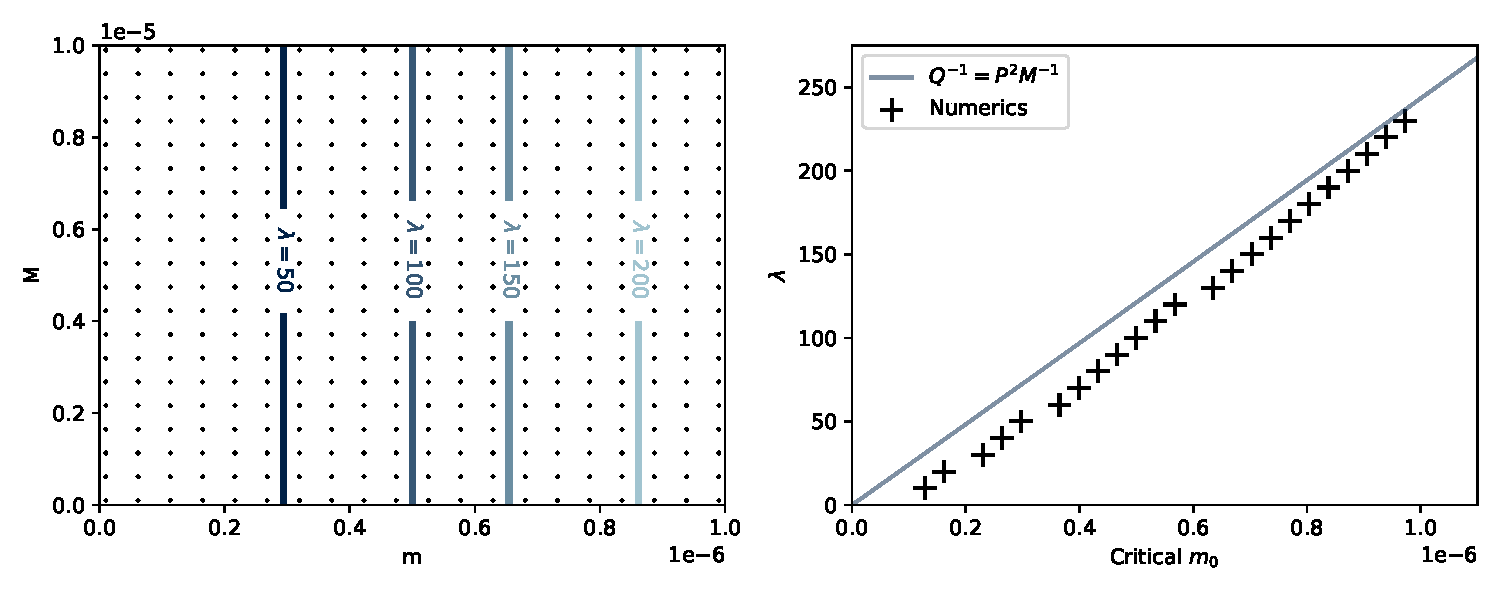
\includegraphics[width=0.9\textwidth]{figures/4-agg-figs/numinus1sidebyside.pdf}
    \caption{Length Dependent Clearance}
    \label{fig:4-numinus1}
\end{figure}

\section{Transitions to Disease and Therapeutic Scenarios}

The reduced model of the aggregation kinetics provides a powerful framework to unify experimental observations and to discuss key features of the the transition to the disease. In both of the reduced models and generalisations (plotted in Figs. (\ref{fig:4-flowConstClear}), (\ref{fig:4-flowMM_P}) and  (\ref{fig:4-generalReduced}) below) there exists a boundary in the $M-m_0$ space that separates systems that will undergo unbound aggregation and those that will have a long term finite aggregate mass. In samples from autopsies, diseased tissue contains cells that are saturated with aggregates. In our model the diseased cells correspond to unbounded aggregation and thus the onset of the disease corresponds to crossing this boundary. \todo{how many cells aggregated etc.} \todo{At some point should I include the exponential proliferation plot?} Each cell in a brain region will likely have different exact physical conditions that may cause slight variations between the exact reaction rates, clearance parameters and monomer concentrations. For example, spatial proximity to blood vessels or the lymphatic system might affect clearance mechanisms, the exact pressure of the internal cellular environment will affect reaction rates and cell-to-cell variability in gene expression will cause the monomer concentrations in different cells to vary \todo{are these good examples + references}. This variability means that each cell will have a slightly different stability line in the $M-m_0$ space. If the system parameters change slightly, then some of the cells may cross the stability line and transition into the unbound aggregation state and ultimately trigger the disease.

\subsection{Ageing reduces Clearance}
\cite{keller_decreased_2000}
A cell in the healthy state can transition to a diseased state if the rate of in vivo clearance mechanisms reduce. For example ageing, or other long term stress on the immune system, might reduce the concentration of the intermediary clearance species, or blood flow in the brain, corresponding to a reduction in the saturating clearance rate, $\lambda_M$ in the model in equation (\ref{eq:4-reducedMM}). This moves the critical line and in particular the value of the monomer concentration at which the bifurcation occurs, $m_0^{(crit)}$. A previously healthy cell with monomer concentration greater than the new critical value, $m_0 > m_0^{(crit)}$, will have transitioned into the disease state and will accumulate aggregates.

The delay before this transition occurs depends on the value of $m_0$ of a cell and how close that is to the initial bifurcation point, $m_0^{(crit)}$ as well as the rate of clearance decline. Individuals with genetic disorders that increase $m_0$ show an earlier onset of disease \todo{ref and discuss more} and impact from sports of other vocations which we expect to reduce clearance more rapidly also show a younger onset of disease \todo{ref and discuss more}.

\subsection{Explaining Genetic Susceptibility}

AD has a high heritability, suggesting there is a genetic component that can cause predisposition to development of the disease in a wide range of adults \cite{bellenguez_genetics_2020}. Genome-wide association studies correlate AD with a variety of gene sets, with the main implications being associations with amyloid/tau and microglia \cite{bellenguez_new_2022}. As discussed, changes in the quantity and quality of monomer protein expression can increase susceptibility to disease. The microglia are cells that support immune function and endocytosis with the brain, directly affecting the clearance mechanisms. These genetic studies do not provide mechanistic insight into the causes of disease, but rather suggest where to look. It is encouraging that two major features that determined the transition to disease in the model developed here, the monomer concentration and clearance mechanisms, were also identified as risk factors in human populations. Despite this currently being a very broad association, quantifying the rate parameters and the effects of mutations will hopefully make major strides towards understand and preventing the onset of the disease in humans.

AD has a reported higher prevalence in individuals with Down Syndrome (DS) \cite{head_aging_2012, zigman_alzheimers_2007}. Although harder to diagnose due to other \todo{impairements}, upto $55\%$ of DS adults aged 40-49 years may be clinically demented and almost all adults with DS over the age of 40 years have neuropatholigcal changes, for example $\beta$-amyloid (A$\beta$) \todo{AB vs BA?} plaques and neurofibrillary tangles, that would lead to a diagnosis of AD \cite{zigman_alzheimers_2007}. AD is more prevalent and has an earlier onset in adults with DS (for comparison see Section \ref{subsubsec:onsetage}). Alongside affecting immune responses, the additional copy of chromosome 21 (which is the genetic basis of DS) increases the expression of amyloid precursor protein \cite{head_aging_2012, rumble_amyloid_1989}. The gene coding for amyloid precursor protein is on the long arm of chromosome 21 and so the trisomy can lead to overexpression of this gene and an increased concentration of the aggregating monomer. However, the mechanistic cause of this correlation has not been understood previously. This work gives a mechanistic grounding that explains the early age of AD onset in adults with DS. The increased protein expression moves the cells and tissues closer to the critical point  in Figure \ref{fig:4-flowMM_P}. As such, a smaller reduction in the clearance rate can trigger the transition to disease, resulting in an earlier age of onset.

\subsection{Rational Therapeutic Design}

\todo{Discuss currently available therapeutics}

In addition to explaining the onset of disease, understanding the mechanisms governing neurodegenerative diseases is essential in the rational design of therapeutics. In the kinetic framework discussed here, an effective therapy will transition cells or tissues from the unstable to stable regions and ensure the stability of the aggregate mass in the future.

\begin{figure}
    \centering
    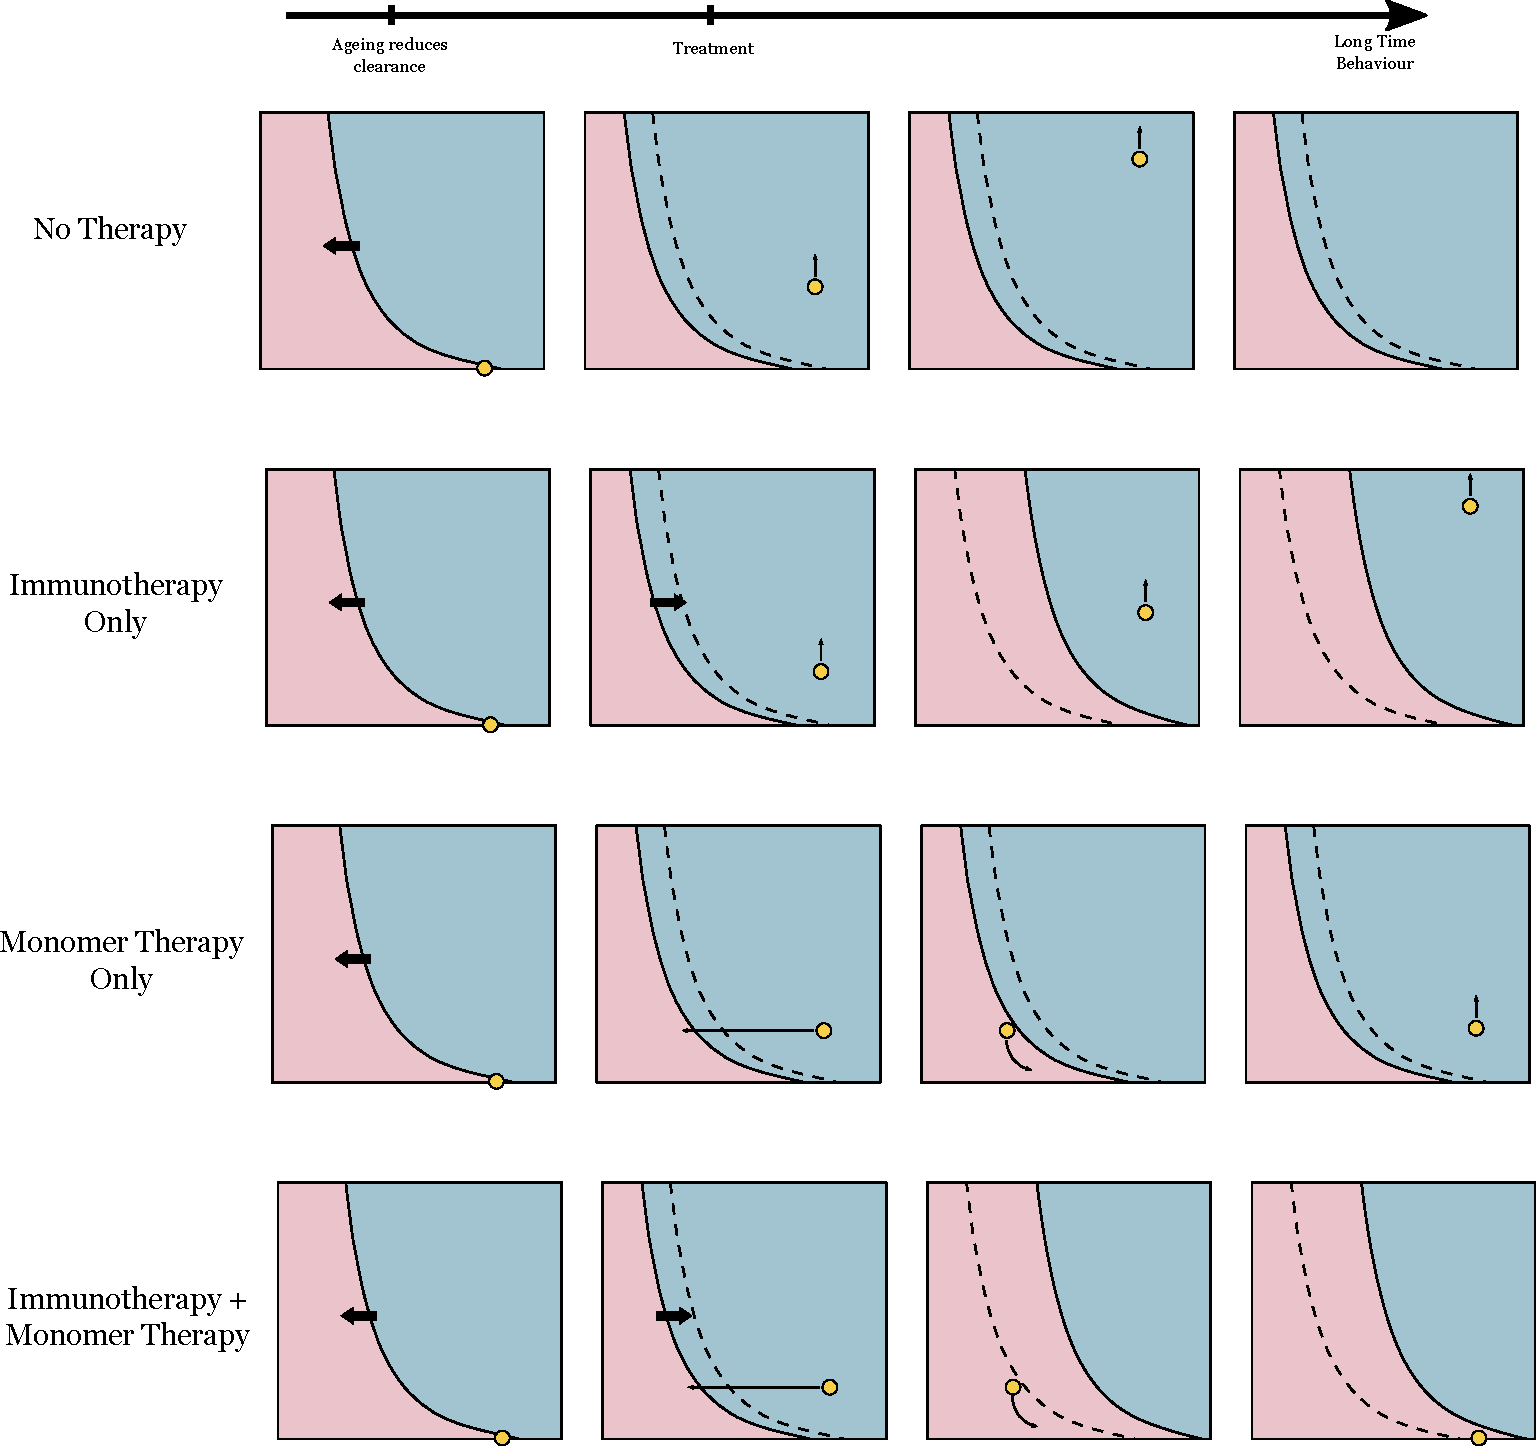
\includegraphics[width=0.9\textwidth]{figures/4-agg-figs/therapyScheme.pdf}
    \caption{Examples of therapeutic schemes.}
    \label{fig:4-therapyscheme}
\end{figure}

The immunotherapy treatments currently under development focus on increasing the clearance mechanisms in the brain. This will shift the balance of aggregation and removal, moving the transition boundary and increasing the area of the stable region. However, since the system will begin proliferating aggregates as soon as it becomes unstable, then the efficacy of the response will depend on how soon any intervention is made after the system become unstable. At early times after the transition, the system will still be close to the stable region, however at later times after more aggregation it will be further from the transition boundary so that the increased clearance does not return the system to being stable. This situation is shown in the second row of Figure \ref{fig:4-therapyscheme}. The best time to take immunotherapy treatments would be before the transition to the unstable region, however it is hard to identify exactly when individuals would become at risk and so hard to design a resource effective treatment strategy at the population level. Furthermore, increasing the population taking medication that may not as susceptible to the onset of disease will also alter the calculation of risks associate side effects of the treatment.

An alternative therapeutic strategy is to develop monomer-reducing therapies, for example ASO-like treatments, or \todo{CHARM system?}. Reducing the monomer concentration can cause an unstable system to cross the transition boundary and return to being stable. The aggregates will then be cleared more quickly than they are produced and the aggregate mass will return to the low stable concentration. However, after some time, the effects of the monomer therapy will reduce and the monomer concentration will return to its original value, once again transitioning into the unstable region so that the aggregates proliferate. This situation is shown in the third row of Figure \ref{fig:4-therapyscheme}. Repeated monomer therapies that act to keep the monomer concentration at some reduced value could keep the system stable, however repeated exposure to ASOs can become toxic \todo{etc etc} and if the protein monomer is functional then reducing its concentration could affect the healthy function of the cell.

An alternative therapeutic strategy that this theory predicts could be a combination therapy of both immunotherapy and monomer reducing therapy. Reducing the monomer ensures an initial transition to the stable region and the subsequent immunotherapy ensures that the system remains in this stable region in the longer term. The final row of Figure \ref{fig:4-therapyscheme} demonstrates how this process will lead to longer term stability. This type of combination therapy would overcome the challenges associated each treatement indivudally, however the exact \todo{need to know the exact sizes of effects etc.}

\section{Summary and Conclusions}


oligomeric proteins reduce transit time between by dissassembling, diffuse more quickly and then reasssembling \cite{agudo-canalejo_cooperatively_2020}

This chapter presents a theory for the kinetics of neurodegenerative diseases that can explain different aspects of the disease into one unified theory. This combines all existing phenomena into one model that 

Unfieid theory, difference regions for different diseases

Could be oligomers that actually cause the disease, but as shown in the first few sections aggregates of all lengths will increase together linearly.

If a lot of small aggregates spread, disease can be triggered below the transition mass -> an argument around the spreading dynamics.

The real need now is to get the parameters in vivo. Talk about randalls data and the fact that time coursing will reveal the role of the two state transition vs stochastic limited nucleation limited aggregation.
\chapter{\label{ch:4-conc}Concluding Remarks} 

\minitoc

%% APPENDICES %% 
% Starts lettered appendices, adds a heading in table of contents, and adds a
%    page that just says "Appendices" to signal the end of your main text.
% \startappendices
% Add or remove any appendices you'd like here:
% \include{text/appendix-1}


%%%%% REFERENCES

% JEM: Quote for the top of references (just like a chapter quote if you're using them).  Comment to skip.
% \begin{savequote}[8cm]
% The first kind of intellectual and artistic personality belongs to the hedgehogs, the second to the foxes \dots
%   \qauthor{--- Sir Isaiah Berlin \cite{berlin_hedgehog_2013}}
% \end{savequote}

\setlength{\baselineskip}{0pt} % JEM: Single-space References

% {\renewcommand*\MakeUppercase[1]{#1}%
% \printbibliography[heading=bibintoc,title={\bibtitle}]}
\printbibliography[heading=bibintoc,title={\bibtitle}]

\end{document}
